\part{临床常见脑病与危象}

\chapter{高血压脑病}

高血压脑病(hypertensive
encephalopathy,HE)是指血压因某种诱因突然显著的增高(原发性或继发性高血压),突破了脑血管的自动调节机制,导致脑血流灌注过多,液体经血脑屏障漏出到血管周围脑组织,导致脑水肿、颅内压增高,而发生的一种急性一过性以神经障碍为主的高血压危象。临床上主要表现有剧烈头痛、烦躁、恶心呕吐、视力障碍、抽搐、意识障碍,甚至昏迷等症状,若不及时救治,常可导致死亡。由于有效防治急进型高血压、急性肾炎和妊娠期高血压病等,本病发生率已有显著下降。

\subsection{病因与发病机制}

高血压是最基本的病因。在此基础上受到某些诱因(如过度劳累、情绪激动、神经紧张、气候变化及内分泌失调等)的激发,或无明显诱因而突然发生血压的急剧升高(舒张压常超过120mmHg),即可导致高血压脑病。临床上以急进型高血压(又称恶性高血压)引起者最常见,其次为急慢性肾炎、肾盂肾炎、子痫、原发性高血压、嗜铬细胞瘤等患者。急性或慢性脊髓损伤患者,因膀胱充盈或胃肠潴留等过度刺激自主神经,可诱发高血压脑病。血压升高的速率对本病的发生也起决定性作用,如急性或新近发生的高血压,可以在慢性高血压患者能够耐受的血压水平上,发生高血压脑病。从血压升高到出现高血压脑病一般需要12~48小时,但也可短至几分钟。

HE是血压急骤升高,发生脑水肿的结果。传统观点认为血压急剧上升时,全身小动脉普遍痉挛收缩,脑小动脉收缩,血管阻力明显增高,脑血流量减少,毛细血管壁由于缺血变性,渗透性增加,使体液和血浆蛋白向血管外渗透加速,从而发生急性脑水肿(脑小动脉痉挛学说)。目前则认为是脑血管“自身调节崩溃”所致。在正常情况下,脑动脉血管的舒缩维持相对的恒定,脑血流量是以脑血管自动调节,主要由血压的高低对血管平滑肌作出相应的反应。当血压低时脑动脉扩张,血压高时脑动脉收缩,以保障大脑组织的血流量供应相对恒定。在正常人,平均动脉压(mean
arterial pressure,MAP,MAP =舒张压+
1/3脉压)在60~120mmHg范围内脑血流量(CBF)保持恒定状态。当正常血压者短时间内突然产生高血压,可在相对较低水平高血压下发生HE,如儿童急性肾小球肾炎等。在慢性高血压患者,由于血压长期缓慢升高,使小动脉壁发生适应性结构改变,即血管壁增厚,管腔狭窄,整个自动调节曲线右移,MAP在120~160mmHg范围内CBF恒定。当MAP
>
160~180mmHg时,便超越了自身调节能力,收缩的血管不能承受这样高的压力,脑小动脉则不能继续收缩,脑动脉自身调节功能降低,继而出现崩溃引起脑动脉被动性或强制性扩张,进入脑的血流量突然增大,灌注量过多而发生脑水肿。毛细血管壁本身变性坏死,继发性点状出血和小灶性梗死,导致脑功能障碍,出现脑病症状。

\subsection{诊断}

\subsubsection{临床表现特点}

HE的病程长短不一,短则几分钟,长则可达数天之久。起病急骤,常因过度劳累、紧张和情绪激动所诱发。病情发展快,进行性加重,发病前常见有血压显著增高,剧烈头痛、恶心、呕吐、精神紊乱等先兆。发病后以脑水肿症状为主,大多数患者具有头痛、抽搐和意识障碍三大特征,称之为HE三联征。头痛常是HE的早期症状,多数为全头痛或额枕部疼痛明显,咳嗽、活动用力时头痛加重,伴有恶心、呕吐,当血压下降后头痛可得以缓解。随着脑水肿进行性加重,于头痛数小时至1~2天后多出现程度不同的意识障碍,如嗜睡、昏睡、木僵、躁动不安、谵妄、定向力障碍、精神错乱,甚至昏迷。若视网膜动脉痉挛时,可有视力模糊、偏盲或黑矇。有时还可出现一过性偏瘫、半身感觉障碍、脑神经瘫痪、甚至失语;亦可见全身性或局限性抽搐等神经系统症状。严重者可出现呼吸中枢衰竭症状。血压多显著升高,舒张压常>
130mmHg,患者多有心动过缓、呼吸困难。长期高血压者可有左心室肥大,心前区可闻及舒张期奔马律,第三心音、第四心音,心电图示有左室劳损。少数病例于脑病后可出现肾功能不全、尿毒症表现。眼底检查有视网膜动脉痉挛,还可有视神经乳头水肿和出血、渗出。脑脊液压力升高(一般不作此项检查,除非必要时,宜选用细针穿刺),化验检查除可有蛋白含量增多和偶有少量红细胞外,余无异常。上述表现常于血压急剧升高12~48小时内明显,若抢救不及时,可于短时间内死亡。

\subsubsection{辅助检查}

颅脑CT扫描可见脑水肿的弥漫性脑白质密度降低,脑室变小;MRI显示脑水肿敏感,呈T\textsubscript{1}
低信号T\textsubscript{2}
高信号,顶枕叶水肿对HE具有特征性,偶见小灶性缺血或出血灶。脑电图常见双侧同步的慢波活动。

\subsubsection{诊断注意事项}

根据患者血压急剧升高后出现上述(头痛、抽搐和意识障碍)神经症状和体征,本病一般不难诊断。但HE为排除性诊断,在确立诊断前,须与脑出血、蛛网膜下腔出血(SAH)、急(慢)性硬膜下血肿、脑栓塞、脑梗死及脑瘤等鉴别。可从以下几点作出判断:

\paragraph{发病情况}

对鉴别诊断很有价值。本病的意识障碍和其他病症多在剧烈头痛发生后数小时才出现,而脑出血、SAH时则多在急剧头痛发生后数分钟至1小时内出现。急、慢性硬膜下血肿患者也有严重头痛,但常有颅脑损伤史,且神经症状体征多在数小时、数日甚至数周逐渐出现。脑梗死尽管起病急,但头痛不明显。脑瘤患者在就诊前常有数周至数月的进行性头痛加重史,其血压升高也不如本病明显。

\paragraph{对降压治疗的反应}

此为重要鉴别点。若予以有效的降压后病情迅速恢复,则支持本病诊断;反之,其他疾病的可能性大。但若本病治疗不及时,使脑组织发生持久性损害,或本病合并尿毒症时,则血压下降后病情恢复较慢或不完全。

\paragraph{眼底检查}

本病有严重的弥漫性或部分性视网膜动脉痉挛,可伴视神经乳头水肿或出血、渗出。脑出血时也可有类似表现。若发生视神经乳头水肿时不伴视网膜动脉痉挛,则提示脑瘤、慢性硬膜下血肿或SAH。视网膜动脉栓塞多提示脑栓塞。

\paragraph{脑脊液检查}

本病的CSF可无或偶有少量红细胞,而脑出血时CSF常为血性,SAH则为明显血性。

\paragraph{颅脑}

CT和(或)MRI检查 可确立诊断。

\subsection{治疗}

当病史和一般检查支持本病诊断时,应立即予以降压治疗,控制血压至安全水平。此时一般不宜花时间去作特殊检查(如CT或MRI检查),以免延误抢救。治疗原则包括紧急降压治疗,制止抽搐和治疗脑水肿,以防发生不可逆的脑损害,注意保护肾功能等。在脑病缓解之后,要积极治疗高血压及引起高血压的原发病,防止HE的复发。

\subsubsection{迅速降低血压}

迅速有效地降低血压是治疗的关键。对HE患者必须在2~4小时之内将血压降至治疗目标值。业已发现,无论正常血压者或高血压患者,脑的自动调节机制下限均约比休息时的MAP低25\%。因此,HE降压治疗的目标值是使MAP降低20\%~25\%,使血压维持在避免高血压危害并保证器官适当灌注的范围。一般要使舒张压迅速降至110mmHg(高血压患者)或80mmHg(血压正常者)以下。在降压过程中要严密监测血压、心率、精神状态,随时调整给药的滴速。另外,要注意因血压降的过快过低,而出现低灌注危象。大多数HE患者的症状随血压的降低而改善,若治疗过程中精神症状没有改善或反而恶化,应重新考虑诊断是否正确并适当升高血压,然后再缓慢降压。常用药物有:

\paragraph{尼卡地平(nicardipine)}

是二氢吡啶类钙拮抗剂。静脉滴注5~10分钟起效,作用持续1~4小时(长时间使用后持续时间可超过12小时),起始剂量为5.0mg/h(可用剂量是5~15mg/h),然后渐增加至达到预期治疗效果;也可直接用2mg静脉注射,快速控制血压后改为静脉滴注。一旦血压稳定于预期水平,一般不需要进一步调整药物剂量。副作用有头痛,恶心、呕吐,面红,反射性心动过速等。尼卡地平能够减轻心脏和脑缺血,对有缺血症状的患者更为有利。尼卡地平治疗HE的特点是:降压作用起效迅速、效果显著、血压控制过程平稳、血压波动小;能有效保护靶器官;用量调节简便;副作用少且症状轻微,停药后不易出现反跳,长期用药也不会产生耐药性,安全性好。与硝普钠相比降压效果近似,而其安全性及对靶器官的保护作用明显优于硝普钠,已成为HE首选药物之一。因其可能诱发反射性心动过速,在治疗合并冠心病的HE时宜加用β受体阻滞剂。

\paragraph{乌拉地尔(urapidil)}

又名压宁定。主要通过阻断突触后膜α\textsubscript{1}
受体而扩张血管,还可以通过激活中枢5-羟色胺-1A受体,降低延髓心血管调节中枢交感神经冲动发放。乌拉地尔扩张静脉的作用大于动脉,并能降低肾血管阻力,对心率无明显影响。其降压平稳,效果显著,有减轻心脏负荷、降低心肌耗氧量、改善心搏出量和心输出量、降低肺动脉压和增加肾血流量等优点,且安全性好,无直立性低血压、反射性心动过速等不良反应,不增加颅内压,不干扰糖、脂肪代谢。肾功能不全可以使用。孕妇、哺乳期禁用。用法:12.5~25mg稀释于20ml生理盐水中静脉注射,监测血压变化,降压效果通常在5分钟内显示;若在10分钟内效果不够满意,可重复静脉注射,最大剂量不超过75mg;继以100~400μg/min持续静脉滴注,或者2~8μg/(kg•min)持续泵入,用药时间一般不超过7天。

\paragraph{拉贝洛尔(labetalol)}

是联合的α和β肾上腺素能受体拮抗剂,静脉用药α和β阻滞的比例为1∶7,多数在肝脏代谢,代谢产物无活性。与纯粹的β阻滞剂不同的是,拉贝洛尔不降低心排血量,心率多保持不变或轻微下降,可降低外周血管阻力,脑、肾和冠状动脉血流保持不变。脂溶性差,很少通过胎盘。静脉注射2~5分钟起效,5~15分钟达高峰,作用持续2~6小时。用法:首次静脉注射20mg,接着20~80mg/10min静脉注射,或者从2mg/min开始静脉滴注,最大累积剂量24小时内300mg,达到血压目标值后改口服。副作用有恶心、乏力,支气管痉挛,心动过缓,直立性低血压等。

\paragraph{其他静脉用降压药物}

酚妥拉明治疗儿茶酚胺过多的高血压急症有良效,如嗜铬细胞瘤、可乐定撤药、可卡因过量等。但因其可增加心肌做功和耗氧量,故禁用于心肌梗死的患者。硝普钠、硝酸甘油能直接增加脑血流量,因此一般不用于HE的患者。

\subsubsection{制止抽搐}

有抽搐者,可用地西泮(安定)10~20mg直接静脉注射,同时肌注苯巴比妥0.2g。如发生癫痫持续状态,其治疗详见本书第85章“癫痫与癫痫持续状态”部分。

\subsubsection{降低颅内压、减轻脑水肿}

可选用20\%甘露醇液250ml静注或快速静滴,依病情每4~8小时1次,可辅以应用呋塞米(速尿)、地塞米松等。详见本书第41章“颅高压危象”部分。

\subsubsection{对症支持疗法}

包括吸氧,卧床休息,保持环境安静,严密观察病情变化,维持水电解质平衡,防治心肾等并发症等。参见有关章节。
\protect\hypertarget{text00098.html}{}{}

\hypertarget{text00098.htmlux5cux23CHP4-1-4}{}
参 考 文 献

1.
郭树彬.高血压急症的处理与靶器官保护策略.中国急救医学,2009,29(1):76

2. 田国祥
,孟庆义.高血压急症治疗-尼卡地平的兴起.中国循证心血管医学杂志,2010,2(1):6

3. Rodriguez MA,Kumar SK,De Caro M. Hypertensive crisis. Curr Drug
Targets,2009,10(8):788

\protect\hypertarget{text00099.html}{}{}

\chapter{肺 性 脑 病}

肺性脑病(pulmonaryencephlopathy)是由慢性胸肺疾患伴有呼吸衰竭,出现缺氧与二氧化碳(CO\textsubscript{2}
)潴留而引起以精神及神经系统症状为主要表现的一种综合征。突出表现为严重呼吸性酸中毒、自主呼吸减弱及中枢神经系统功能障碍的精神神经症状。

肺性脑病是我国独特应用的疾病诊断名词,相当于国际文献所称的“二氧化碳麻醉(carbon
dioxide narcosis)”,主要病因是由于严重的CO\textsubscript{2}
潴留。广义的肺性脑病是指由于肺功能障碍所引起的脑部症状,包括高碳酸血症和低氧性及过度通气所致的脑部症状等。狭义的肺性脑病是指由通气功能不全所致的动脉血CO\textsubscript{2}
急性潴留或慢性潴留加重时所产生的脑部神经系统症状,可伴有不同程度的缺氧,属于低氧血症合并高碳酸血症的Ⅱ型呼吸衰竭。

本症是慢性胸肺疾病的一个严重并发症,常伴有程度不同的多脏器损害,病死率高达30\%以上。

\subsection{病因与发病机制}

慢性阻塞性肺疾病(COPD)为肺性脑病的基础病因,以慢性肺心病所致者多见。导致肺性脑病的常见诱因有:①急性呼吸道与肺部感染,严重支气管痉挛,气道内痰液阻塞,使原已受损的肺通气功能进一步下降致体内CO\textsubscript{2}
潴留。②医源性因素,如镇静剂应用不当,高浓度吸氧,导致呼吸抑制而加重CO\textsubscript{2}
麻醉状态;不适当应用脱水剂及利尿剂,致痰液黏稠而加重气道阻塞。③慢性阻塞性肺疾病伴有右心衰竭时,由于脑血流量减少,加重脑缺氧及脑代谢功能紊乱。

肺性脑病的发病机制尚未完全阐明,但目前认为低氧血症、CO\textsubscript{2}
潴留和酸中毒三个因素共同损伤脑血管和脑细胞是最根本的发病机制。

脑组织耗氧量大,约占全身耗氧量的1/5~1/4。中枢皮质神经元细胞对缺氧最为敏感。通常完全停止供氧4~5分钟即可引起不可逆的脑损害。对中枢神经影响的程度与缺氧的程度和发生速度有关。当PaO\textsubscript{2}
降至60mmHg时,可以出现注意力不集中、智力和视力轻度减退;当PaO\textsubscript{2}
迅速降至40~50mmHg以下时,会引起一系列神经精神症状,如头痛、不安、定向与记忆力障碍、精神错乱、嗜睡;低于30mmHg时,神志丧失乃至昏迷;PaO\textsubscript{2}
< 20mmHg时,只需数分钟即可造成神经细胞不可逆性损伤。

慢性胸肺疾患严重呼吸衰竭时,肺泡通气功能极度下降,呼吸道中气流阻力增加,致使肺内CO\textsubscript{2}
排出障碍而在肺泡内潴留;血中CO\textsubscript{2}
增加和潴留,体内缺氧,降低了主要缓冲系统BHCO\textsubscript{3}
/H\textsubscript{2} CO\textsubscript{3}
的比值(正常为20∶1)而使血中pH下降。当pH下降到7.35以下,PaCO\textsubscript{2}
升高到70mmHg时,临床就出现呼吸性酸中毒;若PaCO\textsubscript{2} >
80~90mmHg,pH < 7.35,加上CO\textsubscript{2}
潴留使脑血管扩张、脑血流量增加,以及脑血管壁通透性增强,引起颅内压增高及脑水肿,临床病例早期常表现为头痛(晚上加重)、白天嗜睡、晚上失眠、多汗以及皮质中枢兴奋表现,如易激动、烦躁等精神症状;PaCO\textsubscript{2}
> 120~130mmHg,pH <
7.15时,则出现皮质中枢抑制状态,表情淡漠、神志恍惚、精神错乱,出现昏迷,即所谓CO\textsubscript{2}
麻醉状态。然而,临床观察表明,肺性脑病的发生与CO\textsubscript{2}
潴留的急缓有密切关系:CO\textsubscript{2}
在短期内急剧潴留,易诱发肺性脑病;CO\textsubscript{2}
缓慢潴留不易发生肺性脑病;且与脑脊液(CSF)pH直接相关。有时观察到血pH很低时,CSF
pH并不低,患者清醒;若患者血pH不低而CSF
pH很低,则患者意识障碍;表明患者意识障碍与CSF
pH明显降低呈正相关,而和血pH不相关。可能的原因是,{}
和H\textsuperscript{+} 缓慢地通过血脑屏障,而CO\textsubscript{2}
能较迅速地通过血脑屏障和细胞膜,在脑组织内、毛细血管和CSF中很快平衡,使CSF的PaCO\textsubscript{2}
在短时间急剧升高,CSF的pH迅速下降,从而造成动脉血与CSF中的pH出现不一致的CSF酸中毒,导致患者意识障碍,神志不清。而在慢性CO\textsubscript{2}
潴留时,PaCO\textsubscript{2}
虽然增高,但由于CSF中的HCO\textsubscript{3} \textsuperscript{−}
能逐渐代偿,促使CSF
pH维持在正常范围,则不宜发生肺性脑病。因此,肺性脑病的发生与CSF
PaCO\textsubscript{2} 急剧上升和CSF的pH迅速下降呈正相关。

缺氧及CO\textsubscript{2}
潴留均会使脑血管扩张,血流阻力降低,血流量增加以代偿脑缺氧。缺氧和酸中毒还能损伤血管内皮细胞使其通透性增高,导致脑间质水肿;缺氧使细胞ATP生成减少,造成Na\textsuperscript{+}
-K\textsuperscript{+}
泵功能障碍,离子经细胞膜的正常转运功能遭到破坏,因钠泵不能运转,以致钾离子从细胞内移出而进入组织间隙和血液,而Na\textsuperscript{+}
和H\textsuperscript{+} 则进入细胞内取代K\textsuperscript{+}
,结果导致细胞内H\textsuperscript{+}
浓度增加,加重细胞内酸中毒,由于细胞内Na\textsuperscript{+}
增加与进入细胞内的Cl\textsuperscript{−}
结合成NaCl,则引起细胞内渗透压升高,细胞外水分进入细胞内,结果致细胞内Na\textsuperscript{+}
及水增多,形成脑细胞水肿。以上情况均可引起脑组织充血、水肿和颅内压增高,压迫脑血管,进一步加重脑缺血、缺氧,形成恶性循环,严重时出现脑疝。另外,神经细胞内的酸中毒可引起抑制性神经递质γ-氨基丁酸生成增多,加重中枢神经系统的功能和代谢障碍。

肺性脑病还与严重缺氧时的肝、肾功能障碍和体内氨基酸代谢失衡有关。所以当芳香族氨基酸增多、支链氨基酸降低时,因脑组织的芳香族氨基酸增多而导致假神经递质的合成,影响脑的正常功能。

\subsection{诊断}

\subsubsection{临床表现特点}

\paragraph{基础疾病的表现}

有慢性胸肺疾患伴呼吸衰竭的表现。

\paragraph{CO\textsubscript{2} 潴留的神经系统表现}

症状与PaCO\textsubscript{2}
上升的速度及pH下降程度密切相关。早期轻症患者有头痛、头胀、烦躁、恶心呕吐,视力、记忆力和判断力减退;睡眠规律改变(白天嗜睡不醒,夜间失眠、惊醒);继之有神志恍惚、谵语、幻觉、精神错乱、抓空摸床、无意识动作和抽搐、扑翼样震颤;逐渐出现昏迷,眼底视神经乳头水肿,眼球突出,球结合膜充血水肿,出现锥体束征,对各种刺激无反应,脑疝形成等。

\paragraph{缺氧的神经系统表现}

可引起注意力不集中、定向力减退、头痛、兴奋,继而烦躁、谵妄、肌肉抽搐,神经肌腱反射亢进;中枢神经系统受抑制,伴有神志恍惚、昏迷。

\paragraph{血气分析}

示PCO\textsubscript{2} > 70mmHg,pH常小于7.25。

\subsubsection{临床分型与分级}

\paragraph{临床分型}

根据其神经精神症状,可将肺性脑病分为三型:①抑制型:以神志淡漠、嗜睡、昏迷等中枢神经抑制状态为主;②兴奋型:以烦躁不安、谵妄、多语等神经兴奋症状为主;③不定型:抑制与兴奋症状交替出现。

\paragraph{临床分级}

①轻型:神志恍惚、淡漠、嗜睡、精神异常或兴奋、多语而无神经系统异常体征者。②中型:浅昏迷、谵妄、躁动,肌肉轻度抽动或语无伦次,对各种刺激反应迟钝、瞳孔对光反应迟钝而无上消化道出血或DIC等并发症。③重型:昏迷或出现癫痫样抽搐,对各种刺激无反应;反射消失或出现病理性神经体征、瞳孔扩大或缩小;可合并上消化道出血、DIC或休克。

\subsubsection{诊断注意事项}

对慢性胸肺疾病,临床病程中出现神经精神症状时,首先应考虑肺性脑病。但出现精神障碍的神经症状者并不全是肺性脑病,临床极易混淆,故应注意与感染中毒性脑病、严重电解质紊乱、脑出血、DIC、脑动脉硬化、单纯型碱中毒等相鉴别。因此,必须详细询问病史、重视体检、眼底检查,特别是结合血气分析、电解质和有关化验测定,谨慎地加以区别。否则,一律或盲目按肺性脑病处理,必然会造成严重后果。

\subsection{治疗}

肺性脑病的病情复杂,并发症多,治疗上应根据致病原因及病情变化的不同阶段,分别对待,关键在于改善通气功能。为此,必须采取以下综合措施。

\subsubsection{正确氧疗}

通过增加吸入氧浓度来纠正患者缺氧状态的治疗方法即为氧疗。氧疗目标是使SaO\textsubscript{2}
上升至90\%以上或PaO\textsubscript{2}
>60mmHg,同时不使PaCO\textsubscript{2} 上升超过10mmHg或pH <
7.25。氧疗无疑能纠正肺性脑病患者的低氧血症,改善高碳酸血症和酸碱平衡。但若氧疗方法和给氧浓度掌握不当,会导致病情加重,甚至危及生命。肺性脑病因呼吸性酸中毒,有严重高碳酸血症,呼吸中枢对CO\textsubscript{2}
刺激不敏感,此时靠低氧刺激颈动脉窦及主动脉弓的化学感受器以兴奋呼吸。若突然吸入高浓度氧,则可使上述化学感受器不敏感,反而致使呼吸抑制,通气量减少,CO\textsubscript{2}
潴留更多,加重呼吸衰竭和肺性脑病病情。因此,对未行机械通气的患者给氧原则仍以持续性、低浓度、低流量为准。一般吸氧浓度为28\%~30\%,氧流量为1~2L/min。鼻导管或鼻塞法是长时间连续低流量给氧常用的方法,吸氧浓度(\%)=
21 + 4 ×氧流量(L/min)。亦可用面罩给氧。

此外,过量吸氧使换气冲动传入到呼吸肌的作用减弱,导致肺泡通气功能障碍,易致所谓的吸氧性呼吸停止。因此,在吸氧的同时配伍呼吸兴奋剂,以利有效通气,便可防止上述情况的发生。

\subsubsection{保持呼吸道通畅、增加通气量、改善CO\textsubscript{2} 潴留}

积极改善通气,纠正缺O\textsubscript{2} 和CO\textsubscript{2}
潴留是抢救肺性脑病的关键性措施。

\paragraph{清除痰液}

肺性脑病由于呼吸道感染,痰多黏稠,影响痰液不易引流或咳出;并因支气管痉挛、黏膜及黏膜下水肿和纤毛破坏,稠痰更不易咳出。可采用以下措施:①痰液黏稠者:可用祛痰剂如溴己新(必嗽平)8mg,每日3次;氨溴索30mg,每日3次;鲜竹沥液10~20ml,每日3次;10\%氯化铵10ml,每日3次;棕色合剂10ml,每日3次,及其他中药止咳祛痰。氨溴索静脉、肌内及皮下注射,成人每次15mg,每日2次;亦可加入液体中静滴。②无效或积痰干结者:可用药物雾化吸入或超声热蒸气雾化吸入治疗。③咳痰无力者:可采用翻身、拍背、体位引流等措施帮助排痰。必要时可在给氧情况下,通过纤维支气管镜吸引气管、支气管内的分泌物。

\paragraph{解除支气管痉挛}

可用各种支气管扩张剂,以茶碱类、皮质激素和β\textsubscript{2}
受体兴奋剂最常用。①氨茶碱:能解除支气管痉挛,兴奋呼吸中枢,增加心排血量和冠脉流量,利尿,增强呼吸肌与膈肌收缩力量,使通气量增加,PaO\textsubscript{2}
上升,PaCO\textsubscript{2}
降低,肺动脉压下降。用法:0.1~0.2g每日3次口服;或用0.125~0.25g加入25\%葡萄糖液20ml中缓慢静注。注射速度≤0.25mg/(kg•min),静脉滴注维持量为0.6~0.8mg/(kg•h),日注射量一般≤1.0g。应注意:本药剂量过大会引起恶心、呕吐等消化道症状,继而可有心悸、兴奋、心律失常、抽搐等;若已有心肌损害、心律失常、癫痫与活动性溃疡病者,不宜用。合用西咪替丁、喹诺酮类、大环内酯类药物等可影响茶碱代谢而使其排泄减慢,应减少用药量。②皮质激素可用甲泼尼龙80~160mg或氢化可的松300~500mg加入液体中静滴。③β\textsubscript{2}
受体兴奋剂:常用的有沙丁胺醇(salbutamol,舒喘灵)、特布他林(terbutaline,博利康尼,喘康速)、福莫特罗(formoterol)、丙卡特罗(procaterol,美喘清)、克仑特罗(clenbuterol,克喘素)等,可酌情选用。

\paragraph{呼吸兴奋剂的应用}

呼吸兴奋剂可刺激呼吸中枢或主动脉弓、颈动脉窦化学感受器,在气道通畅的前提下提高通气量,从而纠正缺氧和促进CO\textsubscript{2}
的排出,减轻CO\textsubscript{2}
潴留,尚能使患者暂时清醒,有利于咳痰、排痰。它须与氧疗、抗感染、解痉和排痰等措施配合使用,方能更好发挥作用。应用时注意以下几点:①气道必须通畅,否则会增加耗氧量;②脑缺氧或脑水肿未纠正而出现频繁抽搐者慎用;伴有高血压、动脉硬化、癫痫的患者慎用;③若停用呼吸兴奋剂最好逐渐减量或延长给药间隔,使患者呼吸中枢兴奋性逐步恢复,不宜突然终止;④应严格掌握呼吸兴奋剂的适应证:它常用于慢性阻塞性肺病伴有呼吸中枢敏感性降低,或应用镇静催眠药、氧疗使低氧刺激消失后引起的呼吸抑制,或肺性脑病氧疗过程中以及机械呼吸撤离前后配合应用;对以肺换气功能障碍为主所导致的呼衰患者不宜使用。既往常用尼可刹米、洛贝林,用量过大可引起不良反应,现已基本不用。取而代之的有多沙普仑(doxapram),常用20~50mg加入液体中静滴,该药对镇静催眠药过量引起的呼吸抑制和COPD并发急性呼衰有显著的呼吸兴奋效果。

纳洛酮是阿片受体阻断剂,有兴奋呼吸中枢作用,可行肌肉或静脉注射,每次0.4~0.8mg,静脉滴注1.2~2.8mg加入5\%葡萄糖液250ml中静脉滴注。

\paragraph{机械通气}

呼吸衰竭时应用机械通气能维持必要的肺泡通气量,降低PaCO\textsubscript{2}
;改善肺的气体交换效能;使呼吸肌得以休息,有利于恢复呼吸肌功能。急性呼吸衰竭患者昏迷逐渐加深,呼吸不规则或出现暂停,呼吸道分泌物增多,咳嗽和吞咽反射明显减弱或消失时,应行气管插管使用机械通气。机械通气过程中应根据血气分析和临床资料调整呼吸机参数。

若患者具备以下基本条件,可行无创正压通气(noninvasive positive pressure
ventilation,NIPPV):①清醒能够合作;②血流动力学稳定;③不需要气管插管保护(即患者无误吸、严重消化道出血、气道分泌物过多且排痰不畅等情况);④无影响使用鼻/面罩的面部创伤;⑤能够耐受鼻/面罩。在COPD急性加重早期给予无创机械通气可以防止呼吸功能不全加重,缓解呼吸肌疲劳,减少后期气管插管率,改善预后。

\subsubsection{控制感染}

呼吸道感染是发生呼吸衰竭进而引起肺性脑病之主要原因。因此,控制呼吸道感染、解除痰液壅塞、改善通气功能,是缓解肺性脑病病情发展和降低病死率的重要环节。肺性脑病患者往往多为老年患者,体弱、反应能力差,临床虽有感染,但表现多不典型。因此,咳嗽、咳黄痰应视为感染征象;肺内呼吸音低、啰音的存在亦应作为判断感染的征象。常见致病菌多为肺炎链球菌、流感嗜血杆菌、卡他莫拉菌、肠杆菌科细菌(肺炎克雷伯菌、大肠埃希菌、变形杆菌等)、铜绿假单胞菌等,或先为病毒感染后继发细菌感染。亦有部分患者为口腔不洁混以厌氧菌感染。应根据痰或呼吸道分泌物细菌培养与药敏,选用有效的抗生素。可供选用的抗菌药物常见的有β-内酰胺/β-内酰胺酶抑制剂(复方阿莫西林、阿莫西林/舒巴坦等)、第二、三代头孢菌素和氟喹诺酮类药物(左氧氟沙星、莫西沙星、环丙沙星)等,或选择具有抗铜绿假单胞菌活性的β-内酰胺类抗生素±氨基糖苷类抗生素。对广谱抗生素使用剂量大、时间较长的病例,尤其是同时使用糖皮质激素者,较易继发真菌感染,应加强口腔护理,每日可用生理盐水清洗口腔2~3次。一旦证实为真菌感染,应给予相应的抑制真菌药物。

\subsubsection{其他治疗}

\paragraph{脑水肿的治疗}

对重症者可以采取轻度或中度脱水,并以缓慢的或中等速度利尿为宜,再辅以冰帽、降温等物理措施。常用制剂为20\%甘露醇1~2g/kg,快速静滴,每日1~2次。也可使用β-七叶皂苷钠5~10mg静注,每日1~2次,或20mg/d加入液体中静滴。肾上腺皮质激素对缺氧所致的脑水肿也有良好的作用。

\paragraph{纠正酸碱平衡失调与电解质紊乱}

①呼吸性酸中毒:在慢性呼吸衰竭中最常见。保持呼吸道通畅,增加肺泡通气量是纠正此型失衡的关键。仅当pH
<
7.20时,可少量补充5\%碳酸氢钠(40~50ml)。②呼吸性酸中毒合并代谢性碱中毒:常见于呼吸性酸中毒的治疗过程中,多为医源性因素所致。处理原则为纠正呼吸性酸中毒的同时,只要每日尿量在500ml以上,可常规补充氯化钾3~5g。若pH过高,可静脉滴注盐酸精氨酸10~20g(加入5\%葡萄糖液500ml中)等。③呼吸性酸中毒合并代谢性酸中毒:常提示病情危重、预后差。处理包括增加肺泡通气量、纠正CO\textsubscript{2}
潴留;治疗引起代谢性酸中毒的病因;适当使用碱剂,补碱的原则同单纯型呼吸性酸中毒,一次可补充5\%碳酸氢钠(80~100ml),以后根据血气,再酌情处理。④呼吸性碱中毒:多因CO\textsubscript{2}
排出过多所致。一般不需特殊处理,以治疗原发病为主。电解质紊乱的处理见本书第6篇“水、电解质和酸碱平衡失调”部分。

\paragraph{防治心力衰竭}

慢性肺心病出现心功能不全以右心衰竭为主。一般经过氧疗、控制呼吸道感染、改善肺功能后,症状可减轻或消失,不需常规使用利尿剂和强心剂。较重者或经上述治疗无效者可选用小剂量缓效利尿剂。氢氯噻嗪25mg,每日1~3次;螺内酯40mg,每日1~2次。对肺性脑病出现脑水肿或重度水肿者可选用呋塞米(速尿)20mg缓慢静脉注射。应注意利尿剂可引起低血钾、低血氯,诱发或加重代谢性碱中毒;利尿过多可致血液浓缩、痰液黏稠加重气道阻塞。当慢性呼吸衰竭伴有左心功能不全时,可考虑适当使用洋地黄类药物。用药原则是选用小剂量(常规用量的1/2~1/3)、作用快、排泄快的强心剂。常以毛花苷丙(西地兰)0.2~0.4mg或毒毛花苷K
0.125~0.25mg加入葡萄糖液20ml内缓慢静脉注射(20分钟)。应注意纠正缺氧、防治低血钾,不宜依据心率的快慢观察疗效。如患者血压稳定,可考虑使用血管紧张素转化酶抑制剂治疗。

\paragraph{镇静剂的应用}

对肺性脑病患者的谵妄、狂躁不安和精神症状,在排除代谢性碱中毒后,应着重改善肺泡通气,避免用能加重呼吸抑制的镇静剂,如吗啡、哌替啶、巴比妥类药物、氯丙嗪等。必要时可用东莨菪碱0.3~0.6mg肌注,或地西泮10mg肌注。亦可用中成药醒脑静注射液(安宫牛黄注射液)2~4ml肌注。

\paragraph{脑细胞代谢与保护剂的应用}

如细胞色素C、辅酶A、ATP、胞磷胆碱、脑活素、纳洛酮等。

\paragraph{支持疗法}

可酌情输给血浆、复方氨基酸及人体白蛋白,以增强机体抵抗力。补给维生素B、C等。

\paragraph{防治并发症}

包括心力衰竭、休克、上消化道出血、DIC等,详见有关章节。
\protect\hypertarget{text00100.html}{}{}

\hypertarget{text00100.htmlux5cux23CHP4-2-4}{}
参 考 文 献

1. Hodgkin JE. Chronic obstructive pulmonary disease. Clin Chest
Med,1990,11:363

2. 陆再英,钟南山.内科学.第7版,北京:人民卫生出版社,2008:141

3. 秦桂玺 ,阎明.急危重症病与急救.北京:人民卫生出版社,2005:340

4. 俞森洋
,蔡柏蔷.呼吸内科主治医生660问.第2版.北京:中国协和医科大学出版社,2009:453

\protect\hypertarget{text00101.html}{}{}

\chapter{肝 性 脑 病}

肝性脑病(hepatic
encephalopathy,HE)是由严重肝病引起的以代谢紊乱为基础的、意识障碍、行为失常和昏迷为主要表现的中枢神经系统功能失调综合征。既往曾称肝昏迷(hepatic
coma),目前认为肝昏迷是HE程度相当严重的第四期,并不代表HE的全部。其发生是多种因素综合作用的结果,发病机制涉及氨中毒、假性神经递质、血浆氨基酸失衡、γ-氨基丁酸(GABA)、硫醇增多、短链脂肪酸代谢紊乱和星形细胞功能异常等学说,但主要原因是因肝细胞功能衰竭(肝细胞弥漫病变)和来自胃肠道未被肝细胞代谢去毒的物质经体循环(肝内外分流)至脑部而引起。

既往认为,重症肝炎或药物中毒所致者,起病急剧并进行性加重,称为急性肝性脑病;其中呈暴发性过程,短期内出现意识障碍者,又称为暴发性肝功能衰竭(fulminant
hepatic
failure,FHF)。它系由于肝脏大块或广泛坏死,残存肝细胞不能代偿生物代谢作用,代谢失衡或代谢毒物不能有效的被清除,导致中枢神经系统的功能紊乱,故亦称为内源性HE,或非氨性HE。此型HE,由于肝细胞广泛坏死所致,故预后极差。慢性肝性脑病是指严重慢性肝病(如肝硬化、原发性肝癌)及(或)门-体分流术后,从肠道中吸收入门脉系统的毒性物质,通过分流未经肝脏的首次通过作用(first
pass
effect)进入体循环,引起中枢神经系统的功能紊乱,因而亦称为外源性HE,或氨性脑病,或称为门-体分流性脑病(porto-systemic
encephalopathy,PSE)。本型HE约50\%有诱因,消除诱因后,可使病情逆转,预后较好。急性肝性脑病(内源性HE)与慢性肝性脑病(外源性HE),无论在临床上或发病机制上,有时均难以截然区别。以前将无明显临床表现和生化异常,仅能用精细的智力实验和(或)电生理检测才能作出诊断的HE,称为亚临床HE(subclinical
HE,SHE)或隐性HE(latent
HE,LHE)。由于概念不清易被理解为发病机制不同的另外一种病症,故目前主张用轻微HE(mild
HE,MHE)较为合适(见下述)。

最近(2002年)国际消化病学大会(world congress of
gastroenterology,WCOG)工作小组将HE分为A、B和C三型,实际上也恰好取了分别代表急性(acute)、分流(bypass)和肝硬化(cirrhosis)的英文首字母以便记忆。

A型肝性脑病,即急性肝功能衰竭相关的HE(acute liver failure
associated-HE,ALFA-HE),用来代替原来代表一种急性HE的FHF的术语,因为FHF实际的意义远不仅指急性HE。采用ALFA-HE能够避免将急性肝功能衰竭伴发的HE与慢性肝病伴发的急性HE的概念进一步混淆。

B型肝性脑病,是存在明显门体分流但无内在肝病的脑病。很少见,分流的原因可以包括先天性血管畸形和在肝内或肝外水平门静脉血管的部分阻塞以及各种压迫产生的门静脉高压,而造成门体旁路。此时肝活组织检查提示肝组织学正常,但临床表现与肝硬化伴HE的患者相同。因此,只有在肝活检显示为正常的肝组织学特征,才能诊断这种类型的脑病。此外,特异性的确认此类型有助于医生诊断不明确的疾病。

C型肝性脑病,指在慢性肝病或肝硬化基础上发生的HE,不论其临床表现是否急性。包括了绝大多数的HE,即通常意义上的HE。认为肝功能不全是C型发生的主要因素,而循环分流居于次要地位,但两者可协同作用。沿用的“门体分流性脑病”基本都是此型。根据HE的不同表现、持续时间和特点,C型又可以分成发作性、持续性和轻微HE
3个亚型:

\hypertarget{text00101.htmlux5cux23CHP4-3-1}{}
(1) 发作性HE:

是在慢性肝病的基础上在短期内出现意识障碍或认知改变,不能用先前存在的有关精神异常来解释,并可在短期内自行缓解或在药物治疗后缓解。发作性HE根据有无诱因又可分为:①诱因型:有明确的可追踪的诱发因素;②自发型:无明确的诱发因素;③复发型:指1年内有2次或2次以上HE发作。

\hypertarget{text00101.htmlux5cux23CHP4-3-2}{}
(2) 持续性HE:

是在慢性肝病的基础上出现持续性的神经精神异常,包括认知力下降,意识障碍,昏迷甚至死亡。根据患者自制力和自律性受损的严重程度可进一步分为:①轻型:即HEⅠ级;②重型:即HEⅡ~Ⅳ级;③治疗依赖型:经药物治疗可迅速缓解,若间断治疗,症状又会加重。

\hypertarget{text00101.htmlux5cux23CHP4-3-3}{}
(3) 轻微(minimal)HE:

是指某些慢性肝病的患者无明显症状性HE(发作性或持续性HE的临床表现和生化异常),但用精细的智力实验和(或)神经电生理检测可见智力、神经、精神的异常而诊断的HE。轻微HE在肝硬化患者中的患病率约为30\%~80\%。此型越来越受到重视,因为患者虽形似正常,但操作能力和应急反应能力减低,在从事高空作业、机械或驾驶等工作时容易发生意外。以往所用的“亚临床HE”或“隐性HE”这个词有一定的误导性,易被误认为其发病机制独立于HE之外或临床意义不大,故近年已接受改称为轻微HE,以强调其作为HE发展过程中的一个特殊阶段。

\subsection{病因与发病机制}

\subsubsection{病因与诱因}

\paragraph{病因}

各种严重的急性和慢性肝病(病毒性肝炎肝硬化最多见)均可伴发肝性脑病。急性肝病时肝性脑病的病因是由于大量的肝细胞坏死,常为病毒性肝炎、药物或毒素引起的肝炎;也可由于大量肝细胞变性,如妊娠期脂肪肝、Reye综合征等。慢性肝病,如肝硬化和重症慢性活动性肝炎的肝性脑病是由于有功能的肝细胞总数减少和肝血流改变;慢性肝性脑病的发病与广泛的门-体静脉分流有关。肝脏被恶性肿瘤细胞广泛浸润时,也可导致肝性脑病。

\paragraph{诱因}

许多因素可促发或加剧肝性脑病(表\ref{tab38-1}),此种情况在慢性肝病时尤为明显。常见诱因有:①上消化道出血:尤其是食管静脉及胃底冠状静脉曲张破裂出血,是慢性肝性脑病最常见的诱因;急性胃黏膜病变出血则是急、慢性HE共有的常见诱因。②利尿剂使用不当或大量放腹水。③高蛋白饮食。④应用镇静安眠药(巴比妥类、氯丙嗪等)以及麻醉剂等。⑤给予含氨药物(氯化铵)、含硫药物(蛋氨酸、甲硫氨基酸、胱氨酸等)、输注库血、富含芳香族氨基酸的复合氨基酸注射液以及水解蛋白等。⑥感染:如自发性细菌性腹膜炎、脓毒症、肺炎以及泌尿系感染等。⑦电解质紊乱与酸碱平衡失调:常见者为低钠、低钾、低氯、碱中毒。⑧功能性肾衰竭。⑨其他:手术创伤、便秘或腹泻。无诱因的自发性肝性脑病往往是肝硬化的终末期表现,患者肝脏大多缩小,肝功能严重损伤,黄疸深,腹水多,预后恶劣。

\begin{table}[htbp]
\centering
\caption{肝性脑病的诱因及其机制}
\label{tab38-1}
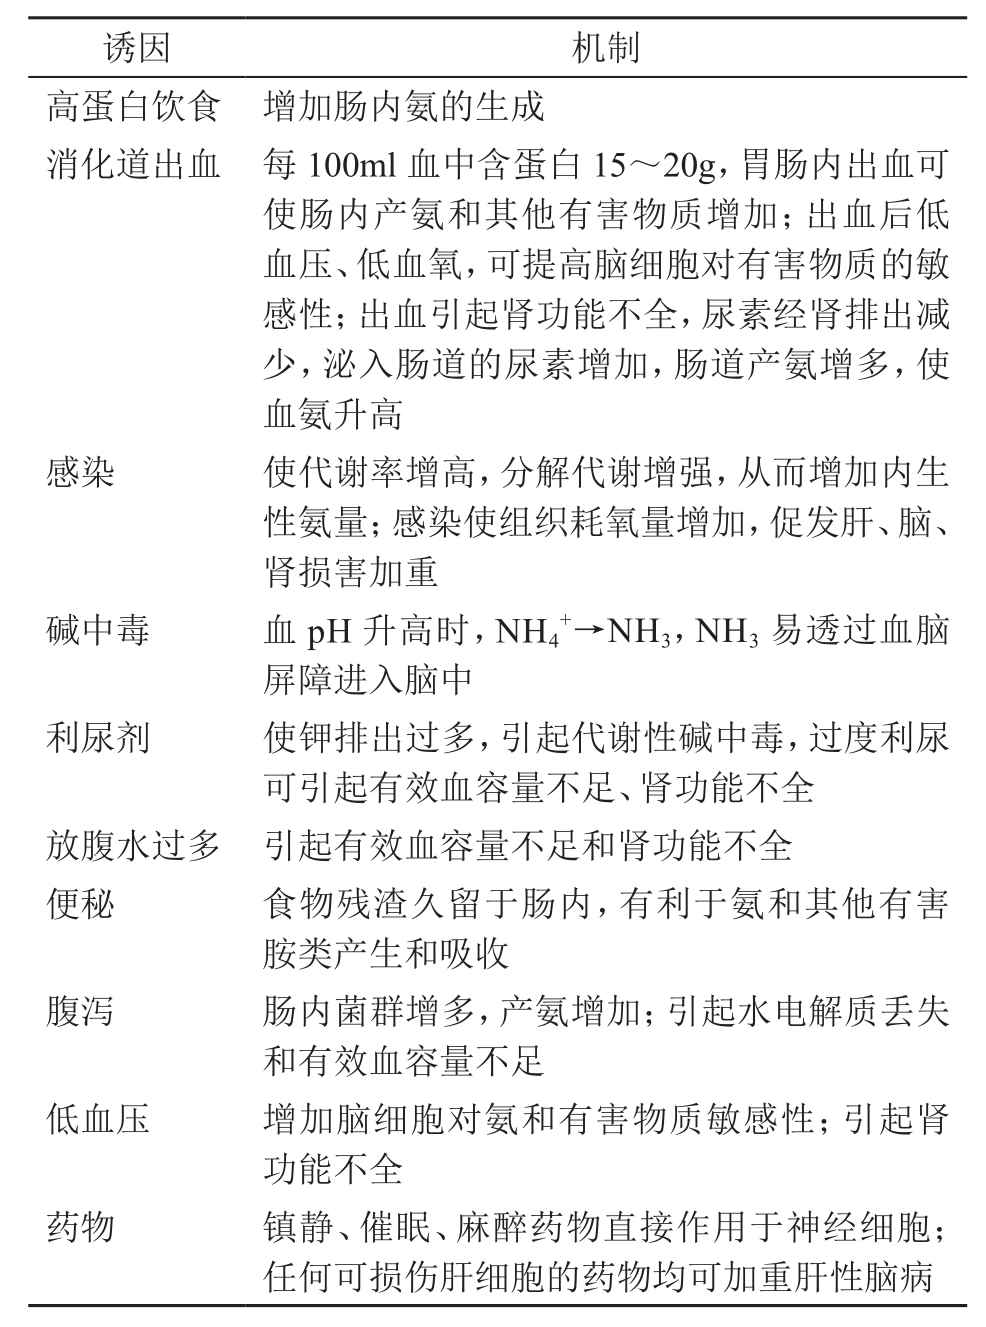
\includegraphics[width=3.28125in,height=4.41667in]{./images/Image00148.jpg}
\end{table}

\subsubsection{发病机制}

肝性脑病的发病机制迄今尚未彻底阐明。一般认为产生HE的病理生理基础是肝细胞功能衰竭和门腔静脉之间有自然形成或手术造成的侧支分流。主要来自肠道的许多可影响神经活性的毒性产物,未被肝脏解毒和清除,经侧支进入体循环,透过血脑屏障而至脑部,引起大脑功能紊乱。虽然氨中毒学说在HE的发病机制中一直占有支配地位,但目前尚没有一种学说能完备的解释HE发病机制的全貌。由于肝脏是机体代谢的中枢,它所引起的代谢紊乱涉及多种环节和途径,因此HE的发病机制也是多因素综合作用的结果。

\hypertarget{text00101.htmlux5cux23CHP4-3-4-2-1}{}
(一) 氨中毒学说

氨中毒学说(ammonia intoxication
hypothesis)在肝性脑病的发病机制中仍占最主要的地位。PET显示肝性脑病患者血氨水平增高,血脑屏障对氨的通透表面积增大及大脑氨的代谢增高(\textsuperscript{13}
NH\textsubscript{3}
-PET)。严重肝脏疾病时,血氨增加的原因是由于氨的生成与吸收增加及(或)清除不足所致。

\paragraph{氨的生成与吸收增加}

①外源性产氨增加:指氨的来源为肠道含氮物质的分解代谢与吸收增加。肠道蛋白质的分解产物氨基酸,部分经肠道细菌的氨基酸氧化酶分解产生氨;另外,血液中的尿素约有25\%经胃肠黏膜血管弥散到肠腔内,经细菌尿素酶的作用而形成氨,后者再经门静脉重新吸收,是为尿素的肠肝循环。肝功能衰竭时,肠道菌丛紊乱且繁殖旺盛,分泌的氨基酸氧化酶及尿素酶增加;同时由于胃肠蠕动和分泌减少,消化和吸收功能低下,使肠内未经消化的蛋白质等成分增多,特别是在高蛋白饮食或上消化道出血后更是如此,以致结肠、小肠内产氨均相应增加;此外慢性肝病晚期,常伴有肾功能下降,血液中的尿素等非蛋白氮含量高于正常,因而弥散到肠腔内的尿素也大大增加,也使产氨增加。肠内氨的吸收决定于肠内容物的pH,pH
> 6时,生成的NH\textsubscript{3} 大量吸收,血氨增加;pH <
6时,以NH\textsubscript{4} \textsuperscript{+}
形式随粪便排出体外,血氨降低。可见,氨的来源主要取决于肠腔蛋白质及尿素肠肝循环的量,氨的生成取决于细菌酶的作用,氨的吸收则取决于肠腔内的pH。②内源性产氨增加:即体内蛋白质的分解代谢产氨增加。肝功能衰竭时,蛋白质分解代谢占优势,加之焦虑、烦躁等情况,肌肉及脑活动均增加,产氨量相应增加。

\paragraph{氨的清除不足}

氨在体内主要经肝脏内鸟氨酸循环合成尿素而被清除;其次在外周组织(如脑、肌肉)先后与α-酮戊二酸、谷氨酸结合生成谷氨酰胺,再经肾脏作用重新释放出氨,由尿排出。肝功能衰竭时,主要是肝脏消除氨的作用减退,其次为肌肉代谢氨减少,另外肾脏排出的氨亦减少。此外,门体分流存在时,肠道的氨未经肝脏解毒而直接进入体循环,亦可使血氨增高。

\paragraph{血氨增加引起脑病的机制}

氨对脑的毒性作用包括:①直接抑制神经细胞膜的电位活动:氨能干扰神经细胞膜上的Na\textsuperscript{+}
-K\textsuperscript{+}
-ATP酶的活性,即破坏血脑屏障的完整性,又损害膜的复极化作用,从而引起HE。②干扰脑的能量代谢:血氨增高使大量α-酮戊二酸转变为谷氨酸,而后者又能转变为谷氨酰胺,故致三羧酸循环中α-酮戊二酸耗竭,循环速度下降,高能磷酸盐和氧耗减低;同时在此过程中消耗大量的ATP和还原型辅酶Ⅰ(NADH),后者减少致呼吸链中的递氢过程受到阻碍,使ATP的生成亦减少;此外,氨还可通过促进磷酸果糖激酶的活性增加,使脑组织内糖酵解过程增强,并直接抑制丙酮酸脱羧酶与有氧代谢,从而增加乳酸的生成,减少ATP的产生。上述生化反应使脑组织中的ATP生成减少,脑组织生理活动受到影响并出现脑病。③增加了脑对中性氨基酸如酪氨酸、苯丙氨酸、色氨酸的摄取,这些物质对脑功能具有抑制作用。④脑星形胶质细胞功能受损:脑星形胶质细胞是氨神经毒性的主要靶细胞。脑星形胶质细胞含有谷氨酰胺合成酶,可促进氨与谷氨酸合成为谷氨酰胺,当脑内氨浓度增加,星形胶质细胞合成的谷氨酰胺增加。谷氨酰胺是一种很强的细胞内渗透剂,其增加不仅导致星形胶质细胞肿胀、功能受损,而且也使神经元细胞肿胀,这是HE时脑水肿发生的重要原因。星形胶质细胞为神经元提供乳酸、α-酮戊二酸、谷氨酰胺及丙氨酸等营养物质,其功能受损可以直接影响神经元的功能及代谢,并参与HE的发生发展过程。⑤通过PET研究发现PSE患者脑氨代谢率升高,氨从血中极易转移到脑中,因此即使血氨正常也会发生脑功能障碍,这可以部分解释血氨不高情况下发生HE以及降氨治疗不一定能完全达到预期目的原因。此外,血氨及其代谢的异常与其他发病机制有协同作用。

\hypertarget{text00101.htmlux5cux23CHP4-3-4-2-2}{}
(二) 脑星形胶质细胞功能异常学说

正常情况下突触前神经末梢释放的谷氨酸迅速被周围的星形胶质细胞摄取,并在谷氨酰胺合成酶的作用下与氨合成为谷氨酰胺,谷氨酰胺再循环至神经元内释放具有活性的谷氨酸,此谓脑中的谷氨酰胺循环。由于脑内缺乏鸟氨酸循环的酶,故脑内清除氨的主要途径依靠谷氨酰胺合成,故谷氨酸氨基化生成谷氨酰胺的“解氨毒”作用完成于星形胶质细胞。另外,谷氨酸是脑内重要的兴奋性神经递质,储存于突触小泡内,一旦释放即呈现神经递质的活性,能与其受体结合产生神经传导活性。而谷氨酰胺是一种很强的细胞内渗透剂,其增加可导致星形胶质细胞肿胀、功能受损。HE时,超量的氨经谷氨酰胺合成酶的作用,不仅使具有活性的谷氨酸形成减少,导致谷氨酸能突触异常,还耗费了大量能量,并可导致谷氨酰胺的蓄积使胞内渗透压增加使细胞肿胀,肿胀的星形胶质细胞的功能受损进一步影响氨的代谢和谷氨酸活性,出现HE的表现。

\hypertarget{text00101.htmlux5cux23CHP4-3-4-2-3}{}
(三) 假性神经递质学说

神经冲动的传导是通过递质来完成的。正常时兴奋与抑制两类递质保持生理平衡。兴奋性神经递质有儿茶酚胺中的多巴胺和去甲肾上腺素、乙酰胆碱、谷氨酸和门冬氨酸等;抑制性神经递质β-羟酪胺、苯乙醇胺等只在脑内形成。

食物中的芳香族氨基酸如苯丙氨酸及酪氨酸,经肠菌脱羧酶的作用生成苯乙胺及酪胺,该两种胺类正常在肝内被分解清除。严重肝病时,该两种物质在肝内清除发生障碍,经门-体侧支循环进入体循环,并透过血脑屏障进入脑组织,经β羟化酶的作用,分别生成苯乙醇胺和β-羟酪胺。这两种胺的化学结构与正常神经递质去甲肾上腺素极为相似,但不具有正常递质传递神经冲动的作用或作用很弱,因此称其为假性神经递质(false
neurotransmitters)。当假递质被脑细胞摄取并在神经突触堆积至一定程度时,则排挤或取代正常的真递质,使神经传导发生障碍,特别是影响脑干网状结构上行激活系统和大脑边缘系统的神经传递,从而造成精神障碍和昏迷。

但近年来研究结果并不支持假性神经递质学说,如给实验动物静脉注射β-羟酪胺或脑室内注入大量假性神经递质导致脑内β-羟酪胺浓度非常高,脑内去甲肾上腺素和多巴胺明显耗尽,并未引起昏迷;尸检研究发现死于肝性脑病的肝硬化患者脑内去甲肾上腺素和多巴胺水平增加,而β-羟酪胺浓度降低。因此,该学说已逐渐被氨基酸失衡学说(amino
acid imbalance hypothesis)所替代。

\hypertarget{text00101.htmlux5cux23CHP4-3-4-2-4}{}
(四) 氨基酸失衡学说

血浆氨基酸测定发现,某些晚期慢性肝病与HE患者,血浆芳香族氨基酸(AAA)包括酪氨酸、苯丙氨酸、游离色氨酸增高,支链氨基酸(BCAA)包括亮氨酸、异亮氨酸、缬氨酸减少,致血浆氨基酸比值异常。正常人血浆BCAA/AAA的比值为3.5
±
1.0(s),肝性脑病时比值下降至1.0~1.5左右,甚至低于1.0,其下降值与脑病程度有一定的相关性。

血浆氨基酸比值的变化是由于严重肝病所继发的高胰岛素和高胰高血糖素血症所致。在严重肝病时,肝脏对许多激素包括胰岛素、胰高血糖素的灭活作用减弱,使两者血中浓度均增高,但以胰高血糖素的增多更显著,使血中胰岛素/胰高血糖素比值降低,使体内的分解代谢增强。其中胰高血糖素的增多,使组织的蛋白分解代谢增强,致使大量AAA由肝和肌肉释放入血。AAA主要在肝脏降解,肝功能严重障碍,一方面致AAA的降解能力降低,另一方面肝脏的糖异生作用障碍致使AAA转为糖的能力降低,这些均可使血中AAA含量增高。正常时支链氨基酸不被肝脏代谢,主要被肌肉摄取利用,胰岛素有增加肌肉组织摄取和分解利用支链氨基酸的作用,所以当血中的胰岛素水平增高时,促使BCAA大量进入肌肉组织,故血中BCAA浓度减少。AAA和BCAA彼此竞争血脑屏障的同一载体而转运至脑组织内(竞争性抑制)。正常时,血中BCAA的浓度高,竞争力强,从而抑制AAA进入脑内的速度;肝功能衰竭时,由于血浆BCAA减少,高浓度的AAA不受抑制地迅速通过血脑屏障进入脑组织,故脑组织细胞内的AAA含量明显增加。

正常时,脑神经细胞内的苯丙氨酸在苯丙氨酸羟化酶作用下,生成酪氨酸;酪氨酸在酪氨酸羟化酶作用下生成多巴;多巴在多巴脱羧酶作用下生成多巴胺;多巴胺在多巴胺β-羟化酶作用下生成去甲肾上腺素,这是正常神经递质的生成过程。

当进入脑内的苯丙氨酸和酪氨酸增多时,增多的苯丙氨酸可抑制酪氨酸羟化酶的活性,使正常神经递质生成减少。增多的苯丙氨酸可在AAA脱羧酶作用下生成苯乙胺,进一步在β-羟化酶作用下生成苯乙醇胺。而增多的酪氨酸也可在AAA脱羧酶作用下生成酪胺,进一步在β-羟化酶作用下生成β-羟酪胺。因而,苯丙氨酸和酪氨酸进入脑内增多的结果可使脑内产生大量假性神经递质,而产生的假性神经递质又可进一步抑制正常神经递质的产生过程。

氨基酸失衡学说实际上是假性神经递质学说的补充和发展。但下列观察不支持该假说,如临床上发现血浆BCAA/AAA变化和肝性脑病程度并不一定有平行关系;临床上采用静脉或口服BCAA治疗对改善与逆转肝性脑病不一定有效。因此该假说也不能完整地阐明HE的发病机制。

\hypertarget{text00101.htmlux5cux23CHP4-3-4-2-5}{}
(五) GABA/Bz复合受体学说

γ-氨基丁酸(γ-aminobutyric
acid,GABA)是哺乳动物大脑主要的抑制性神经递质。脑内的GABA在突触前神经元内由谷氨酸经脱羟酶(GADI)催化下脱羟生成,并贮存在突触前神经元的囊泡内,此时无生物活性。只有被释放到突触间隙,并结合到突触后神经元膜面特异性的GABA受体上,引起氯离子(Cl\textsuperscript{−}
)转运通道开放,使Cl\textsuperscript{−}
经神经元细胞膜裂隙进入细胞质,原先静止的细胞膜电位即处于高极化状态,从而导致GABA神经递质起明显的突触后抑制作用。突触后神经元膜面的GABA受体不仅能与GABA结合,在受体表面的不同部位也能与巴比妥类(BARB)和苯二氮{}
类(benzodiazepines,Bz,即弱安定类)物质结合,故称为GABA/Bz复合受体或超级受体复合物。该复合受体包括三种配体,即GABA、Bz及BARB配体,彼此有协同性非竞争性结合位点,已证明GABA可引起Bz及BARB的催眠作用,反之亦然,故巴比妥类药能增加GABA的效应。Bz、BARB及GABA受体复合物的连接,通过增加GABA引起的Cl\textsuperscript{−}
通道开放而加强受体复合物对GABA的反应。

大脑抑制性神经递质GABA/Bz的增加可能是导致HE的重要原因。其机制可能有:①血浆内的GABA主要来源于肠道,系谷氨酸经肠道细菌酶作用催化而成。正常时肝脏能大量摄取来自门静脉的GABA,并迅速分解。在肝功能不全时,肝脏对GABA的清除明显减低,血浆内浓度因而明显增高。如果此时血脑屏障对血浆GABA透过性增加,而GABA又不能被神经元分解或摄取,则GABA可抵达GABA受体,使GABA能性神经传递增强。②肝功能不全时中枢神经系统GABA能活性增强尚可以是超级受体复合物上GABA受体密度和(或)亲和力增加的后果。无论GABA、Bz及BARB中任何一种与复合受体结合后,都能促进氯离子由神经元胞膜的离子通道进入突触后神经元的细胞质,使膜超极化,引起神经传导抑制。如有学者研究了动物和人体肝性脑病脑内GABA和Bz受体的数量和亲和性,在一些急性肝性脑病模型中,这些受体的数量成倍增加,而在其他模型中没有变化,这可能提示此时大脑对GABA能神经抑制性调节比Bz或BARB药物更为敏感;PET扫描揭示,脑病患者Bz复合物连接部位增加2~3倍,这可能是肝硬化时脑对镇静药敏感性增加的机制。但近年的研究表明,脑内GABA/Bz的浓度在HE时并没有改变,但在氨的作用下,脑星形胶质细胞Bz受体表达上调。临床上,肝功能衰竭患者对苯二氮{}
类镇静药及巴比妥类安眠药极为敏感,而Bz拮抗剂如氟马西尼对部分HE患者具有苏醒作用,支持该学说。

\hypertarget{text00101.htmlux5cux23CHP4-3-4-2-6}{}
(六) 其他

1.锰的毒性学说
MRI显示80\%以上的肝硬化患者大脑苍白球密度增高,组织学证实是锰沉积而造成的。肝脏是锰排泄的重要器官,当其功能受到影响或存在门体分流时均可使血锰浓度升高,并在苍白球沉积。锰沉积除直接对脑组织造成损伤外,还影响5-羟色胺、去甲肾上腺素和GABA等神经递质的功能。锰还影响多巴胺受体的结合,导致多巴胺氧化使多巴胺减少,使患者产生锥体外系的症状和体征。

2.硫醇与短链脂肪酸学说
①硫醇类:蛋氨酸在结肠内受细菌作用形成硫醇、甲基硫醇和二甲硫化物等,由于肝脏解毒功能减退,进入体循环和脑内,在肝性脑病时血浆浓度增高。硫醇类化合物可抑制神经细胞膜的Na\textsuperscript{+}
-K\textsuperscript{+}
-ATP酶,干扰线粒体的电子传递,以及抑制脑内氨的解毒。血中硫醇类浓度增加,从呼吸道呼出增多,医者可嗅到一种特征性气味,是为肝臭。②短链脂肪酸:肝性脑病患者血浆内C\textsubscript{4}
~C\textsubscript{8}
短链脂肪酸增多。它可抑制氧化磷酸化,使脑干网状结构激活系统的ATP和磷酸肌酸贮存减少,改变神经细胞膜的离子流通,从而抑制神经冲动的传递,诱发肝性脑病。

3.褪黑素(melatonin,MT)
MT是由松果腺分泌的一种激素,具有镇静、催眠、神经内分泌免疫调节等多种生理功能。松果腺细胞从血液中吸收色氨酸,经过一系列酶促反应合成MT。肝硬化时血液中色氨酸浓度升高,松果腺合成MT也增多。MT通过较多的途径增强GABA的中枢抑制,如MT可增加脑内GABA含量,2-吲哚MT可协同GABA神经元放电等。

4.内源性阿片类物质、脑中肌醇和磷酸酯浓度减少等变化对HE的发生有一定作用。

肝性脑病的发生与发展,是多种物质生化代谢紊乱的综合作用。Ziere等观察到氨、硫醇与脂肪酸三者间能互相增强毒物的作用,引起脑病。氨与GABA的协同作用,表现为氨对GABA转氨酶有抑制作用,使GABA不能转变成琥珀酸半醛并进而变为琥珀酸进入三羧酸循环,致脑组织中GABA蓄积并导致神经中枢抑制加深。在高氨血症时,可促进血浆中AAA增高,BCAA/AAA比值降低,血脑屏障对AAA转运增强,致使大量AAA进入脑内引起脑病。多种毒物的协同作用,可解释临床上血氨水平与肝性脑病之间不一定平行这一现象,也说明了为什么单纯消除氨毒性不一定均能逆转肝性脑病。

\subsection{诊断}

\subsubsection{病史}

有前述的病因与诱因存在。

\subsubsection{临床表现特点}

肝性脑病的临床表现往往由于肝病的病因、病程缓急、肝功能损害的程度及诱因等不同而表现不一。A型HE与急性肝功能衰竭相关,可无明显诱因,患者在起病数日内即进入昏迷直至死亡,昏迷前可无前驱症状。C型HE多见于肝硬化患者和(或)门腔分流手术后,以慢性反复发作性木僵与昏迷为突出表现,常有诱因,如上消化道出血等。在肝硬化终末期所见的HE起病缓慢,昏迷逐渐加深,最后死亡。最常见的C型HE,除了患者有性格、行为改变(见下述)外,还常有肝功能严重受损的表现,如明显黄疸、出血倾向等,随着疾病的进展,有些患者可并发各种感染、肝肾综合征、脑水肿和心、肾、肺等主要脏器损害,导致低血压、少尿、呼吸衰竭、DIC、昏迷等相应的复杂表现。B型HE少见,其临床症状的产生源自门体分流,故类似C型,但无肝病的表现,或由其导致门体分流的本身疾病的特征。

典型HE较早出现的症状包括性格改变、精神欣快、智力减退、睡眠习惯改变、说话缓慢而含糊、发音单调而低弱,以及不适当的行为等。个性方面的变化最为显著,原属活泼开朗者,则表现为抑郁,原属内向孤僻者,则可表现为欣快。自发性运动的减少、不动地凝视、表情淡漠、答语迟缓而简短,均系早期表现。早期的行为改变只限于有一些“不拘小节”的行为,如乱扔纸屑,随地便溺,寻衣摸床等毫无意思的动作;这些细微的行为改变只有经常接触患者并留心病情变化的医务人员才能觉察。睡眠过久较早出现,并进展至睡眠节律的倒置,白天昏沉嗜睡,夜间兴奋难眠,这提示患者中枢神经系统的兴奋与抑制处于紊乱状态,预示HE的来临,有人称此种现象为迫近昏迷(impending
coma)。智力衰退,可从轻度的器质性精神功能障碍直至明显的精神错乱,并可观察到这些情况逐日发生变化。局灶性障碍多出现于意识清醒者,常系空间性视觉障碍。其在运动方面的障碍最易识别,如构思性运用不能,患者不能用火柴梗或积木构造简单的图案。典型病例可有书写不整齐而出格的情况,每日的书写记录是观察病程演变的良好准绳。患者的运算能力和逻辑思维明显减退,不能区别相似体积、形态、作用及位置的物体,这是患者常在不适宜场所便溺的原因。进一步发展下去,患者出现骚动、不安、躁狂、幻听,有时表现为进行性精神萎靡和完全无力状。嗜睡和兴奋相互交替为特征之一。患者有谵妄和运动性不安,跃起,叫喊,或哭或笑,但对外界刺激仍有反应,再进一步只对强烈而有害的刺激才起反应。当骚动和谵妄加重,嗜睡期延长,逐渐由木僵状态而进入昏迷。

最具有特征性的神经系体征为“扑翼样震颤(flapping
tremor)”,但不是所有患者都出现此种现象,如在一个严重肝病患者出现这种体征,就具有早期诊断意义。但是扑翼样震颤在早期、中期直至完全昏迷前均可出现。所以应在其他症状出现前经常检查有无此种体征才具有早期诊断意义。扑翼样震颤须在一定的体位时才能显露或引出。嘱患者将上肢伸直,手指分开,或腕部过度伸展而前臂固定不动时可出现掌-指及腕关节呈快速的屈曲及伸展运动,每秒钟常达5~9次,且常伴有手指的侧位动作。有时上肢、颈部、面颌、伸出的舌头、紧缩的口以及紧闭的眼睑均被累及,而患者的步态变为共济失调。患者通常呈现双侧性震颤,虽然双侧的动作不一定完全同时发生,一侧的动作可较另侧明显。震颤在昏迷时消失,但偶尔将患者的一肢轻轻举起或移动时,震颤可重新出现。扑翼样震颤也可在尿毒症、呼吸衰竭及严重心力衰竭中见到。患者可取两腿交叉而贴于腹壁的姿势,四肢有交替性的肌肉强直和松弛。早期有肌腱反射亢进和踝阵挛,锥体束征常阳性,握持反应可阳性。局部或全身性抽搐常见于疾病末期。少数病例,尤其是儿童有舞蹈状动作或手足徐动等。肝性脑病时还可出现一种特征性的气味------肝臭,这种气味很难用语言、文字来形容,有人把其描述为鱼腥味、烂苹果味、变质鸡蛋或大蒜样味等。

\subsubsection{辅助检查}

\paragraph{肝病的实验室检查}

因各类型肝病而异,急性HE患者常以血清胆红素、凝血酶原时间异常为主;慢性HE多伴有低白蛋白血症、高γ-球蛋白血症;各型严重肝病的HE大多有一种或数种电解质异常;血清尿素氮、肌酐在伴有肝肾综合征时升高。

\paragraph{血氨测定}

慢性HE患者多有血氨升高,急性HE患者血氨可正常。

\paragraph{血浆氨基酸测定}

芳香氨基酸尤其色氨酸常呈明显增加,支链氨基酸浓度降低,两者比值常倒置。在慢性肝性脑病更明显。目前已少用。

\paragraph{脑脊液检查}

常规检查和压力均正常,谷氨酰胺、谷氨酸、色氨酸和氨浓度可增高。目前已少用。

\paragraph{脑电图(EEG)检查}

早在生化异常或精神异常出现前,脑电图即已有异常,其变化对诊断与预后均有一定意义。正常人的EEG呈α波,每秒8~13次。HE患者的EEG表现为节律变慢。Ⅱ~Ⅲ期患者表现为δ波或三相波,每秒4~7次;昏迷时表现为高波幅的δ波,每秒少于4次。

\paragraph{神经生理测试}

主要是各种诱发电位(EP)的测定,包括视觉诱发电位(VEP)、脑干听觉诱发电位(BAEP)、躯体感觉诱发电位(SSEP)和事件相关电位(ERPs)P300,被认为对MHE的筛选、诊断、疗效观察等方面优于常规EEG检查。最近研究认为,VEP在不同人、不同时期变化太大,缺乏特异性和敏感性,不如简短的心理或智力测试有效。

\paragraph{心理智能测验}

一般将木块图试验(block design)、数字连接试验(number connection
test,NCT A和B)及数字符号试验(digit symbol
test,DST)联合应用。对诊断早期HE最有价值,对Ⅱ级以上HE不适用。分析结果时应考虑年龄、教育程度等影响因素。

\paragraph{影像学检查}

头部CT或MRI检查时,急性HE患者可发现脑水肿,慢性HE患者则可发现有不同程度的脑萎缩。单光子发射计算机断层摄影(SPECT)可显示区域性的脑血流异常,如额颞部及基底节区的局部血流量降低。MRI还可显示基底神经节(苍白球等)T\textsubscript{1}
加权信号增强(可能与锰的积聚有关)。磁共振波谱学(magnetic resonance
spectroscopy,MRS)是一种在高磁场(1.5T)磁共振扫描机上测定活体某些区域代谢物含量的方法。可用于HE的动态监测和评估各种治疗方案的疗效。正电子发射断层摄影术(PET)可以以影像学形式反映脑的特殊生化或生理学过程,其影像主要取决于所用示踪剂。以\textsuperscript{15}
O-H\textsubscript{2} O可测脑血流;\textsuperscript{13}
N可测氨代谢;\textsuperscript{18} F-氟脱氧葡萄糖(\textsuperscript{18}
F-fluorodeoxyglucose)可测葡萄糖代谢。然而,这些检查费用昂贵,限制了应用。

\paragraph{临界视觉闪烁频率(critical fricker-fusion frequency,CFF)检测}

机制为:轻度星形细胞肿胀是HE的病理改变,而星形细胞肿胀(Alzheimer
Ⅱ型)会改变胶质-神经元的信号传导,视网膜胶质细胞在HE时形态学变化与Alzheimer
Ⅱ型星形细胞相似,故视网膜胶质细胞病变可作为HE时大脑胶质星形细胞病变的标志,通过测定临界视觉闪烁频率可定量诊断HE。该方法可用于发现及检测轻微HE。

\subsubsection{肝性脑病的临床分期}

为了观察HE的动态变化,根据意识障碍程度、神经系统表现和脑电图改变,采用West
Haven分法,将HE自轻度的精神改变到深昏迷分为四期(表\ref{tab38-2})。分期有助于早期诊断、预后估计及疗效判断。

但各期之间并无极其明确的界限,故相邻两期症状协同出现的机会比单独出现的为多。

\subsubsection{诊断注意事项}

Ⅰ~Ⅳ期HE的诊断可依据下列异常而建立:①有严重肝病和(或)广泛门体侧支循环形成的基础;②出现精神紊乱、昏睡或昏迷,可引起扑翼样震颤;③有肝性脑病的诱因;④反映肝功能的血生化指标明显异常和(或)血氨增高;⑤脑电图异常。

轻微HE的诊断依据可有:①有严重肝病和(或)广泛门体侧支循环形成的基础;②心理智能测验、诱发电位、头部CT或MRI检查及临界视觉闪烁频率异常。

HE应与下列疾病鉴别:①出现精神症状时应与精神病鉴别:肝病患者常先表现精神症状,极易误诊为精神病,尤多见于急性重型肝炎时。因此,凡有精神症状等应注意检查有无肝病体征(如黄疸、腹水)和作肝功能检测,以免漏误诊。②有扑翼样震颤时,应除外尿毒症、呼吸衰竭、严重心力衰竭和低钾性昏迷。这四种情况下均可引出扑翼样震颤。③已陷入昏迷的HE,应与引起昏迷的其他常见疾病,如脑卒中、颅内感染、尿毒症、糖尿病昏迷、低血糖昏迷及镇静剂中毒等鉴别。④有锥体束征或截瘫时,还应与脑或脊髓肿瘤、脊髓炎鉴别。

\subsection{治疗}

\subsubsection{及早识别及消除HE诱因}

\paragraph{慎用或禁用镇静药和损伤肝功能的药物}

禁用麻醉剂、巴比妥类、氯丙嗪及大剂量地西泮等。有躁狂、抽搐时,宜首选东莨菪碱(每次0.3~0.6mg肌肉注射),其次为抗组织胺药(如异丙嗪12.5~25mg/次肌肉注射,或苯海拉明10~20mg肌肉注射),或小剂量地西泮(5~10mg/次)。

\paragraph{止血和清除肠道积血}

上消化道出血是HE的重要诱因之一。止血措施参见第13章第1节“上消化道出血”治疗部分。清洁肠道可口服轻泻剂,以每日排出软便2~3次为宜,乳果糖、乳梨醇、大黄等均可酌情使用,剂量因人耐受性而异。对于胃肠道积血须立即排出者,可从胃管抽吸或清洁灌肠。灌肠液可用生理盐水500~700ml加适量的食醋,禁用碱性溶液(如肥皂水)灌肠。亦可口服或鼻饲25\%硫酸镁30~60ml导泻。右半结肠是产氨最多的地方,灌肠液应进抵右半结肠,才能有效地清除该处的内容物,并降低该处的pH,减少毒物在该处的生成和吸收。为此,灌肠时患者先采取臀部高位,使灌肠液进抵结肠脾曲,然后向右侧卧,这样才能使药液进入右半结肠。对急性门体分流性脑病昏迷者用乳果糖500ml加入500ml水或生理盐水中保留灌肠30~60分钟,每4~6小时一次,效果好,应作为首选治疗。

\paragraph{纠正电解质及酸碱平衡紊乱}

低钾性碱中毒是肝硬化患者在进食量减少、利尿过度及大量排放腹水后的内环境紊乱,是诱发或加重HE常见原因。因此,应重视患者的营养支持,慎用利尿剂或剂量不宜过大,大量排放腹水时应静脉输入足量的白蛋白以维持有效血容量和防止电解质紊乱。缺钾者补充氯化钾。若每日尿量超过500ml,即使无低钾血症,在输注高渗葡萄糖液或应用大量排钾性利尿剂时,也应于静脉输液中常规补钾,每日氯化钾补充3~6g。如出现明显低钾血症,应每日分次补充氯化钾共6~9g。稀释性低钠血症,以限制入水量为主,酌情静脉滴注28.75\%谷氨酸钠40m(l相当于生理盐水450ml)以补充钠盐,或酌情应用渗透性利尿剂如20\%甘露醇250ml,使排水多于排钠。长期营养不良、吸收不良、低蛋白血症和利尿剂应用可造成低镁血症,临床上可致肌肉兴奋性升高、手足徐动、谵妄和昏迷。如出现这些症状而给予钙剂(如10\%葡萄糖酸钙等)后无改善或反而加重,应考虑低镁血症。可用25\%硫酸镁5~10ml加入液体中静滴,或每次3~5ml深部肌肉注射,每日1~2次。若有门冬氨酸钾镁针剂宜首选,常用20~40ml加入液体中静滴。若患者有代谢性碱中毒,除补充氯化钾外,还可补充盐酸精氨酸。

\begin{table}[htbp]
\centering
\caption{肝性脑病的分期}
\label{tab38-2}
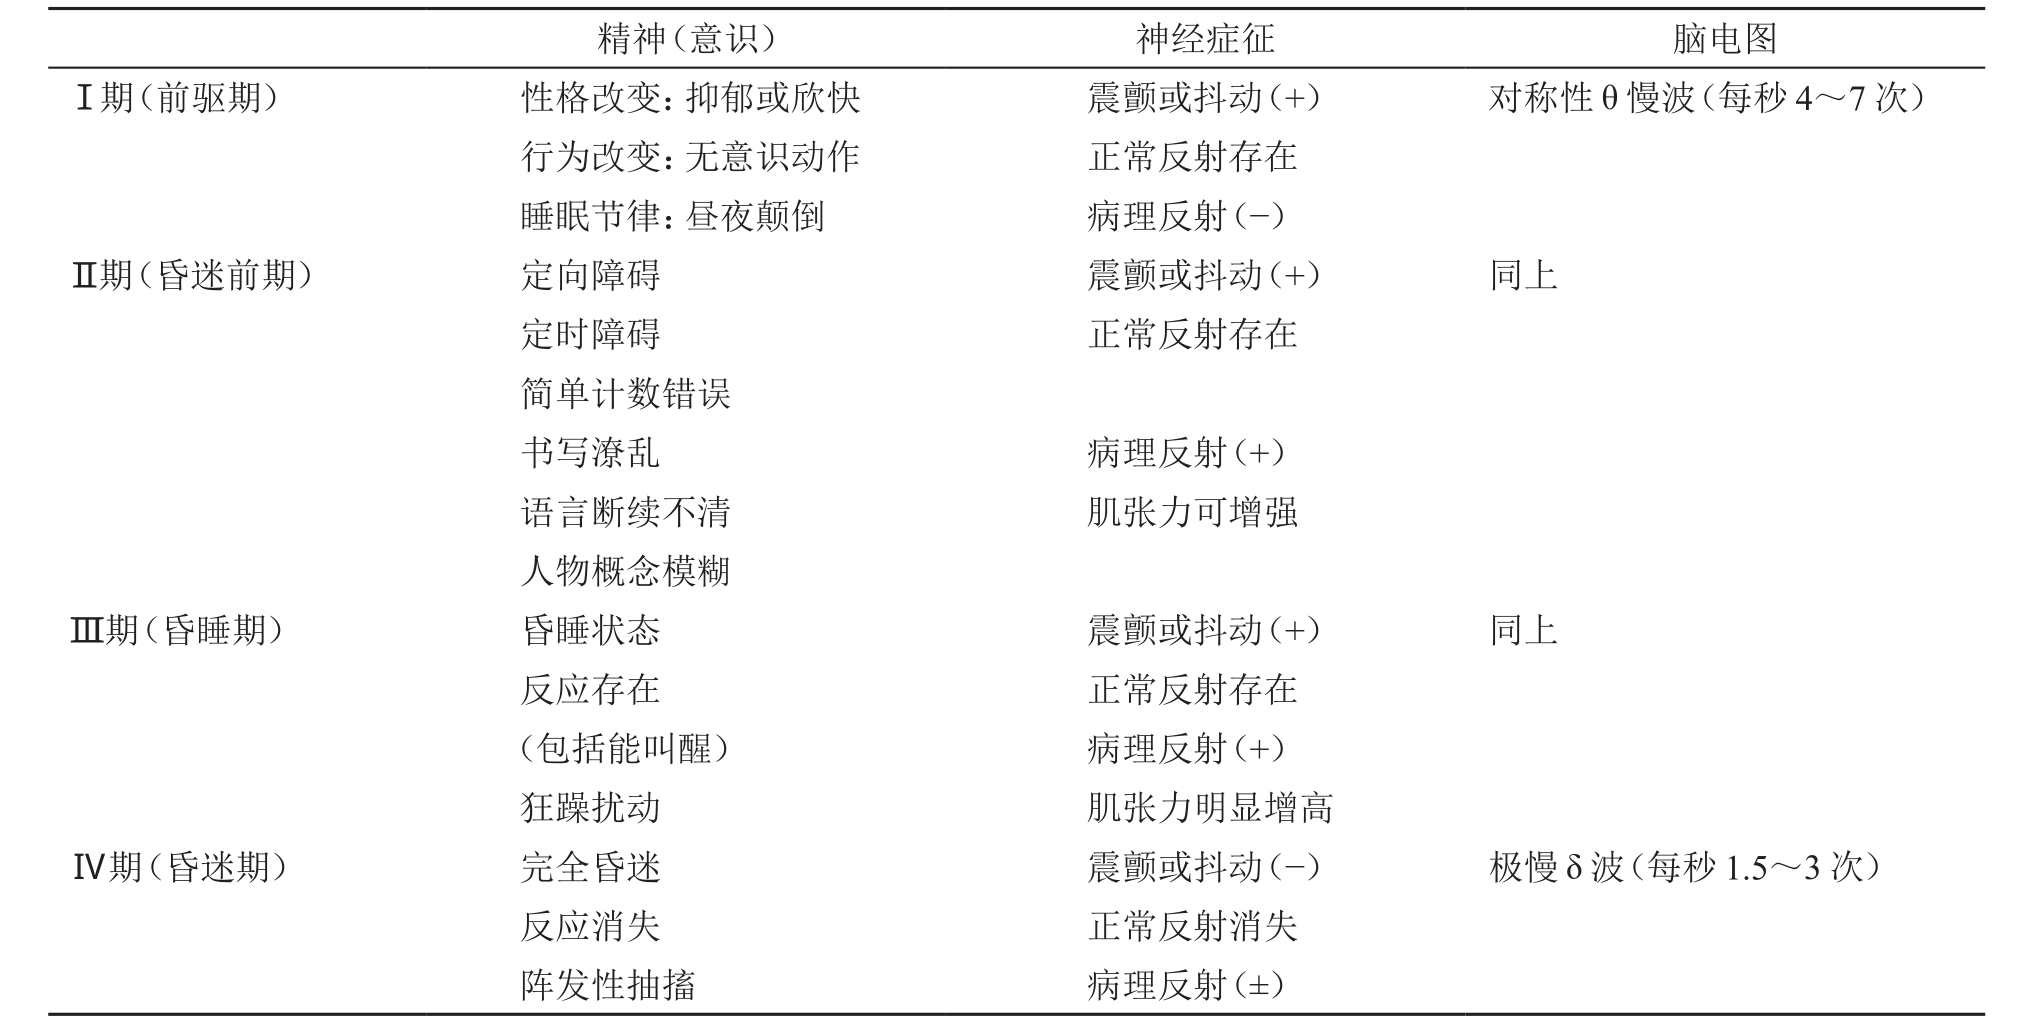
\includegraphics[width=6.78125in,height=3.40625in]{./images/Image00151.jpg}
\end{table}

\paragraph{控制感染}

应选用对肝损害小的广谱抗生素静脉给药。

\subsubsection{减少肠内氮源性毒物的生成与吸收}

\paragraph{控制与调整饮食中的蛋白质}

通常认为,在慢性肝细胞性疾病患者,应予高蛋白饮食,以维持正氮平衡。一旦发生肝性脑病,蛋白质的摄入即应限制并保证热量供给。Ⅲ~Ⅳ期HE患者应禁止从胃肠道补充蛋白质,可鼻饲或静脉注射25\%的葡萄糖溶液。Ⅰ~Ⅱ期患者开始数日应限制蛋白质在20g/d以内,如病情好转,每3~5天可增加10g蛋白质,以逐渐增加对蛋白质的耐受性。待患者完全恢复后每日可摄入0.8~1.0g/kg蛋白质,以维持基本的氮平衡。以植物蛋白为首选,动物蛋白质以乳制品如牛乳或乳酪为佳,如病情稳定可适量摄入。肉类蛋白质应尽量少摄入。少食多餐和睡前加餐可改善机体氮平衡,而不使HE恶化。

但最近的研究显示,与限制蛋白质的摄入相比,正常摄入蛋白1.2g/(kg•d)是安全的,对血氨和HE的恢复无负面影响。在摄入蛋白质的问题上应把握以下原则:①急性期首日患者禁蛋白饮食,给以葡萄糖保证供应能量,昏迷不能进食者可经鼻胃管供食,但短期(4天)禁食不必要;②慢性HE患者无禁食必要;③蛋白质摄入量为1~1.5g/(kg•d);④口服或静脉使用支链氨基酸制剂,可调整AAA/BCAA比值;⑤蛋白质加双糖饮食可增强机体对蛋白质的耐受;⑥植物和奶制品蛋白优于动物蛋白,前者含甲硫氨酸、芳香族氨基酸较少,含支链氨基酸较多,还可提供纤维素,有利于维护结肠的正常菌群及酸化肠道。

\paragraph{清洁肠道}

特别适用于上消化道出血或便秘患者,方法如前述。

\paragraph{抑制肠道菌丛}

肠道中的毒性代谢产物主要是肠道细菌酶作用于基质的结果,控制肠道菌丛,能有效地减少毒性代谢产物的生成。传统方法是给予广谱不吸收性抗生素口服,以减少肠内需氧菌和厌氧菌,使细菌分解蛋白质和尿素减少,从而减少氨的产生,使血氨降低,改善肝性脑病的症状。最常使用的是新霉素,本品从胃肠道吸收很小,仅3\%的口服量随尿排出,在大便中含量高,同时未破坏,故可作为胃肠道抗菌药。口服或鼻饲1.0~1.5g,每日3次。若不能口服时,亦可作保留灌肠,剂量相同,同时每日需做清洁灌肠1~2次。应用新霉素后,多数患者可有神经精神改善,部分患者昏迷清醒,伴有肝臭减轻或消失,动脉血氨下降和脑电图改善。对慢性肝性脑病效果较好。其副作用有:①影响肠黏膜对某些营养物质的吸收(如糖、氨基酸、长链脂肪酸、维生素A、维生素K等),对肠黏膜有一定刺激性并引起其损害;②虽然吸收很少,但仍有约3\%的被吸收,可引起肾及前庭脑神经的损害,血肌酐>
177μmol/L(2mg/dl)时不宜使用;③可引起肠内菌群失调。为此,长期应用宜以小剂量为宜。其他抗菌药物如甲硝唑(灭滴灵,0.8g/d)、氨苄西林、利福昔明(rifaximin)和氟喹诺酮类药物均可选用,可取得相似的效果,但亦应注意其不良反应。其中,利福昔明是一种口服后肠道吸收极少的广谱抗生素(利福平的衍生物),具有起效快、疗效好、耐受性好等优点,可作为Ⅰ~Ⅲ期HE的辅助治疗。抗生素使用期不宜超过1个月,其中急性HE以1~2周为宜,以免引起二重感染等副作用。此外,含有双歧杆菌、乳酸杆菌等的微生态制剂,可起到维持肠道正常菌群,抑制有害菌群,减少毒素吸收的作用。

\paragraph{改变肠道 pH}

常用乳果糖(lactulose)。它是人工合成的含酮双糖,在小肠内不被双糖酶水解,其吸收与排泄均在0.4\%以下,绝大部分进入结肠,主要在右侧结肠内被乳酸杆菌、厌氧杆菌、大肠埃希菌等分解形成乳酸、醋酸和少量甲酸,在结肠内增加发酵,减少腐败,有利于乳酸杆菌的生长。其对肝性脑病的治疗作用主要有:①能有效地降低下段肠内容物之pH。正常情况下,该处pH与血液近似,无梯度存在。应用本品后,由于1分子乳果糖可生成4分子酸,可使该处pH降至5.5以下,右半结肠内pH更低,这样有利于血液中的氨转移至肠腔,并在肠腔内与酸结合而沉淀。②渗透性腹泻作用。由乳果糖分解产生的小分子酸可使渗透压增高,减少结肠内水分吸收,小分子酸又能促进肠蠕动,从而引起腹泻,使粪便在肠腔内停留时间缩短,不利于氨及其他有毒物质的生成与吸收,增加从血液转移至粪便中的氨排出。③改变肠道菌群。肠道乳酸杆菌大量生长,大肠埃希菌和厌氧菌等受到抑制,使氨生成减少。④本品亦可使体内尿素、尿内尿素含量降低,粪内氮质排出增加。每日从胃肠道内尿素释放的氨,相当于25~100g食物蛋白质所释放者,故在降低血氨的情况下,能同时减少体内尿素的含量。⑤本品具有细菌的碳水化合物的底物的作用,能增加细菌对氧的利用,使氨进入细菌的蛋白质中,从而使氨降低。⑥在降低血氨时,可允许患者摄取较多的蛋白质,维持全身营养。乳果糖是目前公认有效的治疗急、慢性肝性脑病的药物,可使临床症状和脑电图均得以改善,对慢性肝性脑病的有效率达90\%,与新霉素合用可提高疗效。新霉素虽能杀灭细菌,但不影响乳果糖所致的肠内pH下降,这是因为新霉素对类杆菌属无作用,而这种细菌分解乳果糖,因而两者合用具有协同作用。

乳果糖有糖浆剂(60\%)和粉剂,可口服或鼻饲,日剂量30~100ml,分3次服用。从小剂量开始,视病情增减,以调整至每日排2~3次软便或糊状便,或使新鲜粪便的pH降至6.0以下。一般在用药后1~7天开始起作用。对不能口服或鼻饲者可予乳果糖灌肠。本品无毒性,很安全,主要的不良反应是腹泻、腹胀、纳差,少数可有呕吐、腹部痉挛性疼痛,可减量或停药后消失。尚有部分患者对其不耐受,因过甜而不喜欢服用。

乳梨醇(lactitol)是另一种双糖(β-半乳糖-山梨醇),系由乳糖还原而制备。作用与疗效和乳果糖类同。价格较乳果糖便宜,甜味也较轻,易于入口,可溶入果汁或水内饮服,易为患者接受。其剂量为每日30~40g,分3次口服。不良反应与乳果糖相同。

对于乳糖酶缺乏者亦可试用乳糖,由于有的人小肠内缺乏乳糖酶,口服乳糖后在小肠不被分解与吸收,进入结肠后被细菌分解而酸化肠道,并产生气体,使肠蠕动增加而促进排便。其剂量为每日100g。

\subsubsection{促进体内氨的代谢}

1.L-鸟氨酸-L-门冬氨酸(ornithine-aspartate,OA)为一种鸟氨酸和门冬氨酸的混合制剂,能促进体内的尿素循环(鸟氨酸循环)而显著降低HE患者血氨。鸟氨酸能增加氨基甲酰磷酸合成酶和鸟氨酸甲酰转移酶活性,其本身也是鸟氨酸循环的重要物质,促进尿素合成。门冬氨酸可促进谷氨酰胺合成酶的活性,促进脑、肝肾的利用和消耗氨以合成谷氨酸和谷氨酰胺而降低血氨。用法:每次口服5g,每天2~3次;静脉滴注10~20g/d,最多不超过80g/d,用量过大易致消化道反应。严重肾功能衰竭者禁用。

2.鸟氨酸 -α-酮戊二酸
鸟氨酸的作用机制如上所述。α-酮戊二酸可增加谷氨酰胺合成酶活性,其本身还是三羧酸循环上的重要物质,能与氨结合形成谷氨酸。其疗效不如OA。

3.苯甲酸钠和苯乙酸钠
苯甲酸钠可与甘氨酸作用产生马尿酸盐,苯乙酸钠可与谷氨酰胺作用形成苯乙酰谷氨酰胺,从尿中排出。排泄一分子的苯甲酸盐,肾脏即可排泄一分子的氮。苯甲酸钠每次口服5g,每日2次,其治疗HE的效果与乳果糖相当,但价格便宜,费用仅为乳果糖的1/30。苯乙酸钠的效果不如苯甲酸钠,但两者之间有协同作用。

4.谷氨酸钠(钾)
在理论上,谷氨酸可与氨结合生成谷氨酰胺而降低血氨。临床上常用28.75\%谷氨酸钠(每支5.75g/20ml,含钠34mmol)40~100ml和(或)31.5\%谷氨酸钾(每支6.3g/20ml,含钾34mmol)20~40ml加入5\%~10\%葡萄糖液中静滴。一般认为钠盐与钾盐混合或交替应用较单纯用钠盐或钾盐为好。谷氨酸钠与钾两者合用比例一般为2~3∶1,低钾时为1∶1。静滴过快可引起流涎、面色潮红、恶心等反应。由于谷氨酸与氨结合生成谷氨酰胺是在ATP与镁离子的参与下进行的,故应同时给予ATP和硫酸镁(或门冬氨酸钾镁)。但谷氨酸不易透过血脑屏障;各种肝病时血浆谷氨酸浓度增高而非降低;谷氨酸盐为碱性(可同时加入5~10g维生素C滴注),可使血pH升高;钠离子可加重腹水和脑水肿,临床上尚无对照研究证明其有肯定疗效。因此,目前倾向于认为此类药物应用价值可疑。

5.盐酸精氨酸
此药偏酸性,有碱血症时可选用。常用量为25\%盐酸精氨酸40~80ml加入液体中静滴。

6.L-卡尼汀(L-carnitine)是广泛存在于机体内的一种特殊氨基酸,是人体长链脂肪酸代谢产生能量必需的一种物质。临床试验证实本品有降低血氨和改善HE的作用。

7.硫酸锌
氨通过尿素循环转化为尿素的过程需要5种酶,其中2种酶是锌依赖性的。由于锌在尿中丢失增加,锌缺乏在肝硬化患者中常见。锌缺乏可诱发复发性HE的发作,加重病情,补充锌后病情缓解,同时锌在DNA和蛋白质合成、含金属酶的功能中具有广泛的重要作用。因此,对锌缺乏的肝硬化患者应予以适当补锌治疗。

\subsubsection{调节神经递质、改善神经传导}

\paragraph{支链氨基酸(BCAA)}

BCAA制剂是一种以亮氨酸、异亮氨酸、缬氨酸等BCAA为主的复合氨基酸。其机制为竞争性抑制芳香族氨基酸进入大脑,减少假神经递质的形成,其疗效尚有争议。现倾向于认为BCAA不宜作为肝性脑病的常规用药,但对治疗某些类型(门-体)脑病可能是有益的;在不能耐受蛋白食物或限制蛋白摄入的患者,为了维持正氮平衡,改善营养,BCAA的应用不仅有指征,也是安全的(BCAA比一般食用蛋白质的致昏迷作用小)。

\paragraph{氟马西尼(flumazenil)}

为GABA/Bz复合受体拮抗剂,对部分Ⅲ、Ⅳ期HE患者有促醒作用。用法为:0.5mg加入0.9\%氯化钠注射液10ml于5分钟内静脉推注完毕,继以1.0mg加入0.9\%氯化钠注射液250ml中静滴(约30分钟)。

\paragraph{阿片受体拮抗剂}

纳洛酮能使HE患者提前清醒,总有效率达90\%,可减少长期昏迷所导致的并发症,并且不良反应少,是治疗HE的有效药物。其机制是:①纳洛酮能消除大量内源性阿片肽释放对心血管功能和呼吸的抑制,改善脑组织微循环。②大剂量的纳洛酮直接作用于脑细胞,保护Na\textsuperscript{+}
-K\textsuperscript{+} -ATP酶,抑制Ca\textsuperscript{2+}
内流、自由基释放及脂质过氧化,从而保护脑细胞,减轻脑水肿。③对抗中枢性神经递质GABA,激活脑干网状结构上行激活系统,有中枢催醒作用。④抑制HE时巨噬细胞的趋化活性,减少炎症反应。⑤改善缺血时神经细胞内Ca\textsuperscript{2+}
、Mg\textsuperscript{2+} 的紊乱,恢复线粒体氧化磷酸化和能量供给。

\paragraph{左旋多巴}

本品为多巴胺的前体。能透过血脑屏障进入脑内,经多巴脱羧酶作用生成多巴胺,进而形成去甲肾上腺素,以排挤假性神经递质,恢复中枢神经系统的正常兴奋性递质,从而恢复神志;它还有提高大脑对氨的耐受性以及增加肝血流量,改善心肾功能使肾排泌氨增加,间接地降低血氨及脑脊液中的氨。用法:0.2~0.4g加入5\%葡萄糖液250ml中静滴,每日1~2次。亦可用2~4g/d,分4~6次口服或鼻饲。通常用药后24~30小时神志改善。由于维生素B\textsubscript{6}
是多巴脱羧酶的辅酶,在周围神经促使左旋多巴更多地变成多巴胺,以致中枢神经系统不能得到神经递质的补充,故在用左旋多巴时,不宜并用维生素B\textsubscript{6}
。既往对本品评价较高,认为其至少对部分患者有效,曾被作为治疗急性肝性脑病的首选药物之一。但随机对照研究显示,无论是口服抑或静脉注射,该药均不能促进昏迷患者苏醒。因此,目前对其疗效的评价持否定态度者居多,已少用。此外,左旋多巴的副作用较多,如:①食欲减退、恶心、呕吐,并使溃疡加重,甚至消化道出血;②烦躁不安、失眠及幻觉;③舌、口唇、面颊、下颌可发生不随意运动;④有拟肾上腺素作用,引起心悸、血压升高和期前收缩等。对有器质性心脏病患者应慎用或禁用。

\paragraph{溴隐亭(bromocriptine)}

为多巴胺受体激动剂,具有增强神经传导、增加脑血流和代谢的作用。开始剂量为2.5mg/d,与饮食同服,每3天增加2.5mg/d,最大剂量为15mg/d,8~12周1疗程,可用于慢性HE对其他治疗无反应者。其副作用有恶心、呕吐、腹绞痛、便秘或腹泻、疲倦、头痛、眩晕等。与左旋多巴一样,其疗效未得肯定,目前少用。

\subsubsection{肝硬化腹水的治疗}

肝硬化腹水形成是门静脉高压和肝功能减退共同作用的结果,为肝硬化肝功能失代偿时最突出的临床表现。肝硬化腹水形成机制主要涉及门静脉压力升高、血浆胶体渗透压下降及有效血容量不足等。

治疗腹水不但可减轻症状,且可防止在腹水基础上发展的一系列并发症如SBP、HRS等。腹水治疗措施如下:

\paragraph{限制钠和水的摄入}

限钠饮食和卧床休息是腹水的基础治疗。钠摄入量限制在60~90mmol/L(相当于食盐1.5~2.0g/d),应用利尿剂时,可适当放宽钠摄入量。有稀释性低钠血症(血钠低于125mmol/L)者,应同时限制水摄入,摄入水量在500~1000ml/d。

\paragraph{利尿剂}

对上述基础治疗无效或腹水较大量者应使用利尿剂。常用螺内酯和呋塞米合用:先用螺内酯40~80mg/d,4~5天后视利尿效果加用呋塞米20~40mg/d,以后再视利尿效果分别逐步加大两药剂量(最大剂量螺内酯400mg/d,呋塞米160mg/d)。理想的利尿效果为每天体重减轻0.3~0.5kg(无水肿者)或0.8~1.0kg(有下肢水肿者)。应监测体重变化及血生化。

\paragraph{提高血浆胶体渗透压}

对低蛋白血症者,每周定期输注白蛋白或血浆,可通过提高血浆胶体渗透压促进腹水消退。

\paragraph{难治性腹水的治疗}

难治性腹水(refractory
ascites)定义为使用最大剂量利尿剂(螺内酯400mg/d加上呋塞米160mg/d)而腹水仍无减退。对于利尿剂使用虽未达最大剂量,腹水无减退且反复诱发HE、低钠血症、高钾血症或高氮质血症者亦被视为难治性腹水。其治疗可选择下列方法:①大量排放腹水加输注白蛋白:在1~2小时内放腹水4~6L,同时输注白蛋白8~10g/L腹水,继续使用适量利尿剂,可重复进行。此法对大量腹水患者,疗效比单纯加大利尿剂剂量效果要好,对部分难治性腹水患者有效。但应注意不宜用于有严重凝血障碍、HE、上消化道出血等情况的患者。②经颈静脉肝内门体分流术(transjugular
intrahepatic portosystemic
shunt,TIPS):该法能有效降低门静脉压,但仅用于上述治疗无效的难治性腹水、肝性胸水及伴肾功能不全者。③肝移植:难治性腹水是肝移植优先考虑的适应证。

\subsubsection{病因治疗}

对A型HE患者,采取综合治疗措施(如抗病毒治疗、促进肝细胞再生等)治疗急性肝功能衰竭;对B型HE患者或C型某些与门体分流相关的自发型HE患者,临床上可用介入治疗技术或手术阻断门-体侧支循环,以降低HE的复发率;C型HE患者,病因治疗的重点是肝移植,包括原位肝移植和肝细胞移植。

\subsubsection{其他治疗}

包括人工肝支持治疗、驱锰治疗、肝移植、放射介入或直接手术的方法阻断门-体侧支循环、积极防治并发症等。

\subsection{预后}

HE的预后主要取决于肝细胞衰竭的程度和诱因是否可被去除。诱因明确且容易消除者(例如出血、缺钾等)的预后较好。肝功能较好,分流手术后由于进食高蛋白而引起PSE者预后较好。有腹水、黄疸、出血倾向的患者提示肝功能很差,其预后也差。暴发性肝功能衰竭所致的HE预后最差。
\protect\hypertarget{text00102.html}{}{}

\hypertarget{text00102.htmlux5cux23CHP4-3-8}{}
参 考 文 献

1.
王宇明.肝性脑病的定义、命名和诊断.中华肝脏病杂志,2004,12(5):305-306

2. Antoni M. Hepatic encephalopathy:from pathophysiology to treatment.
Digestion,2006,73(supplement):S86-93

3. 陈灏珠
,林果为.实用内科学.第13版.北京:人民卫生出版社,2009:2120-2126

4. 张文武 .急诊内科学.第2版.北京:人民卫生出版社,2008:477-492

5. Faint V. The pathophysiology of hepatic encephalopathy. Nurs Crit
Care,2006,2:69

\protect\hypertarget{text00103.html}{}{}

\chapter{低渗性脑病}

低渗性脑病(hypoosmolar
encephalopathy)系指细胞外液呈低渗状态,部分水分移入细胞内而导致脑细胞水肿,从而引起脑的代谢和功能障碍,出现一系列精神神经症状的综合征。

\subsection{病因与发病机制}

血液的渗透压一般可分为晶体渗透压(即一般所指的渗透压)和胶体渗透压,它们各自维持着人体细胞内外水的平衡和血管内外水的平衡。当血浆晶体渗透压降低或增高,则水移至细胞内引起细胞水肿;或水移至细胞外引起细胞脱水,此种改变均在短期内发生即可影响脏器的功能,甚至迅速发生危及生命的病情。而血浆胶体渗透压降低(低蛋白血症)引起的水肿常为慢性过程,不致短期内发生危及生命的病情。人体体液渗透压改变后是由下丘脑部位的渗透压中枢来调整,即当细胞外液(ECF)渗透压和容积增减时,影响下丘脑对内源性抗利尿激素(ADH,即精氨酸加压素AVP)释放和抑制释放,以调整体液容量和渗透压。ADH的作用是增加远端肾小管和集合管对水的通透性,从而使水重吸收增加,如血浆渗透压降低则下丘脑抑制释放ADH,尿量乃增多;反之,则释放ADH,尿量乃减少,这样维持着人体体液容量和渗透压于正常范围。当各种原因使血浆晶体渗透压严重降低时,则引起脏器细胞水肿,其中脑细胞更易受累及。一般说来,低渗状态,成年人是指血浆渗透压<
280mOsm/L,儿童< 270mOsm/L;引起脑病则应进一步降低,如成年人<
260mOsm/L,儿童< 250mOsm/L。

细胞外液低渗最常见原因是低血钠。血钠<
125mmol/L数小时,就可导致脑细胞水肿,形成低渗性脑病;而轻度低血钠,一般不会导致低渗性脑病。在常见的低血钠中,只有稀释性低血钠和缺钠性低血钠可以引起低渗性脑病,尤其是前者。稀释性低血钠最常见于ADH分泌过多,尤其是所谓ADH分泌失调综合征(syndrome
of inappropriate antidiuretic hormone
secretion,SIADH)。SIADH常见病因为:①恶性肿瘤:某些肿瘤组织合成并自主性释放AVP。最多见者为肺燕麦细胞癌,约80\%的SIADH患者是由此引起。其他肿瘤如胰腺癌、淋巴肉瘤、网状细胞肉瘤、十二指肠癌、霍奇金淋巴瘤、胸腺瘤等也可引起SIADH。②呼吸系统疾病:如肺结核、肺炎、阻塞性肺部疾病等有时也可引起SIADH,可能由于肺组织合成与释放AVP。另外,感染的肺组织可异位合成并释放AVP样肽类物质,具有AVP相似的生物特征。③中枢神经系统疾病:包括脑外伤、炎症、出血、肿瘤、多发性神经根炎、SAH等,可影响下丘脑-神经垂体功能,促使AVP释放而不受渗透压等正常调节机制的控制,从而引起SIADH。④药物:如氯磺丙脲、长春新碱、环磷酰胺、卡马西平、氯贝丁酯、三环类抗抑郁药、秋水仙碱等可刺激AVP释放或加强AVP对肾小管的作用,从而产生SIADH。AVP、DDAVP过量时也可造成SIADH。部分病因不明者称之为特发性SIADH。由于AVP释放过多,且不受正常调节机制所控制,肾远曲小管和集合管上皮细胞对水的重吸收增加,尿液不能稀释,游离水不能排出体外,如摄入水过多,水分在体内潴留,细胞外液容量扩张,血液稀释,血清钠浓度与渗透压降低。同时,细胞内液也处于低渗状态,细胞肿胀,当影响脑细胞功能时,可出现神经系统症状。SIADH一般不出现水肿,因为当细胞外液容量扩张到一定程度,可抑制近曲小管对钠的重吸收,使尿钠排出进一步增加,因此,钠代谢处于负平衡状态,加重低钠血症与低渗血症。同时,容量扩张,GFR增加,以及醛固酮分泌受到抑制,也增加尿钠的排出。尿渗透压高于血浆渗透压。

稀释性低血钠也见于肾功能不全时,未加限制地输入大量低渗液和葡萄糖液。缺钠性低血钠多发生于长期限制钠盐摄入,特别是同时应用利尿剂者;呕吐与腹泻也是常见原因。老年人和育龄妇女更易于发生低钠血症的脑损害。研究表明,雌性激素能促进血管加压素从垂体的释放,而雄性激素则能抑制其释放。雌激素和雄激素对脑Na\textsuperscript{+}
-K\textsuperscript{+}
-ATP酶有不同的效力:雌激素能显著降低Na\textsuperscript{+}
-K\textsuperscript{+} -ATP酶的活力,后者则相反,而Na\textsuperscript{+}
-K\textsuperscript{+}
-ATP酶对低钠血症时维持正常的脑容量是十分重要的。正是由于以上两个原因,育龄妇女对罹患低钠血症严重并发症有更高的危险。低渗性脑病的病理改变为脑细胞水肿,细胞间隙小,但常无血管损伤,血脑屏障相对完整。脑细胞水肿较重时则颅压增高,产生颅内压增高的临床表现。严重的颅内压增高导致脑组织向颅内阻力较小的区域移动而疝入硬脑膜间隙或颅骨生理孔道形成脑疝,造成受压脑组织阻碍CSF通路和脑血液循环,使颅内压更形增高,则受压的神经结构淤血、水肿、出血和软化。由于此种改变为细胞内外渗透压差增大所致,故可在补晶体后随渗透压升高能很快纠正,有起病快、恢复快的特点。这不同于脑瘤、炎症的血管源性脑水肿和各种脑积水的间质性脑水肿,此类脑水肿不能较快消除病因,而改善脑水肿或脑病亦较缓慢。

\subsection{诊断}

\subsubsection{具有低渗血症的临床特征}

低渗性脑病是在血浆晶体渗透压降低的基础上发生,故先有低渗血症,严重时发展为低渗性脑病。患者常存在有低钠、低氯、低钾、低钙、低镁和水失调,临床表现有头痛、头晕胀、注意力不集中、体力衰弱、疲乏、肌力降低、常卧床不起、纳差、恶心、呕吐、腹胀、腱反射迟钝等。

\subsubsection{低渗性脑病的临床表现特点}

按细胞外液渗透压降低的程度与临床表现,可将低渗性脑病分为以下三度。

\paragraph{轻度}

成人血浆渗透压为260~250mOsm/L,儿童为250~240mOsm/L,临床上出现表情淡漠、乏力、倦怠、纳差、恶心、腹胀等症状。

\paragraph{中度}

成人渗透压为250~240mOsm/L,儿童为240~230mOsm/L,临床表现为嗜睡、头晕、反应迟钝、定向力障碍等。

\paragraph{重度}

成人渗透压< 240mOsm/L,儿童<
230mOsm/L,临床表现为谵妄、浅昏迷或昏迷、抽搐、周围循环衰竭等,甚至发生脑疝。

\subsubsection{辅助检查}

\paragraph{血浆晶体渗透压测定}

血浆晶体渗透压正常范围为280~300mOsm/L。其测定方法有:①冰点下降法;②晶体计算渗透压法:血浆晶体渗透压由电解质、尿素、葡萄糖等低分子物质组成,故可以计算。公式为:血浆渗透压(mOsm/L)=
2(Na\textsuperscript{+} + K\textsuperscript{+}
)(mmol/L)+葡萄糖(mmol/L)+尿素氮(mmol/L)。根据此公式计算出的血浆渗透压和冰点下降法测定值基本相同。

\paragraph{ADH测定}

任何ADH分泌增加的疾病均可形成稀释性低钠血症,故测定ADH可确定由ADH分泌增多所致的低渗血症。由于ADH主要为使肾小管重吸收水增加,但对Na\textsuperscript{+}
、K\textsuperscript{+} 、Cl\textsuperscript{−}
等电解质的重吸收无明显作用,故尿内排电解质不减少。SIADH的特征为:①血清钠降低(常<
130mmol/L);②尿钠增高(常> 30mmol/L);③血浆渗透压降低(常<
270mOsm/L);④尿渗透压>血浆渗透压;⑤有关原发病或用药史;⑥血浆AVP增高对SIADH的诊断有重要意义。在正常情况下,当细胞外液处于低渗状态,AVP的释放被抑制,血浆AVP常明显降低或测不到;但在SIADH患者,血浆AVP常不适当增高;⑦无水肿,肾功能、肾上腺皮质功能正常。ADH正常值波动较大,主要和人体水负荷有关。正常参考值为1.0~9.2pg/ml,平均3.65pg/ml。

\paragraph{尿渗透压测定}

采用冰点下降法。也可采用尿比重粗略估计,即比重1.005 =
200mOsm/L,每增加0.05则渗透压增加200mOsm/L,如1.010 = 400mOsm/L,1.015 =
600mOsm/L,1.020 =
800mOsm/L,故ADH分泌正常的低渗血症尿比重低于1.010,SIADH的低渗血症因尿钠排出不减少,其渗透压在300~400mOsm/L以上,即尿比重高于1.010。

\paragraph{红细胞体积(MCV)和血细胞比容(Hct)测定}

低渗血症水移向细胞内而致MCV和Hct增大,可间接判断血浆渗透压。

\paragraph{低渗性脑病的有关检查}

低渗性脑病的诊断首先须有血浆渗透压降低,其次需有脑病的临床表现及实验室检查异常。这些辅助检查包括视乳头水肿、脑脊液压力增高、脑电图可出现广泛性慢波、颅脑CT扫描常无异常病变等,结合临床病情,有助于低渗性脑病的诊断。

\subsubsection{诊断注意事项}

\paragraph{单纯(ADH分泌正常者)低渗血症和ADH分泌增加低渗血症的鉴别}

如前所述,低渗血症可由缺钠性低钠血症和由SIADH水潴留引起的稀释性低钠血症所引起,两者的病因、病情不一,且治疗时SIADH性低渗血症还应限制入水量,故应予以鉴别。

\paragraph{低渗性脑病和肺性脑病的鉴别}

在肺心病Ⅱ型呼吸衰竭患者,常伴发有低渗血症和肺性脑病,此类病例仅纠正呼吸衰竭或仅纠正低渗血症常不能明显改善病情,只有针对两者并治才能有效。尤其是要注意低渗性脑病和肺性脑病的并存,或误将低渗性脑病作为肺性脑病来处理的情况。

\paragraph{低渗性脑病和其他脑病}

、脑水肿疾患的鉴别
脑病和脑水肿可由多种病因引起,也有部分病例初为其他原因引起,后因治疗不当促使低渗性脑病的发生。故不论何种原因的脑病,均应将血浆渗透压作为常规检查,以便及时发现低渗血症和低渗性脑病。

\subsection{治疗}

\subsubsection{病因治疗}

纠正基础疾病,药物引起SIADH者需立即停药。地美环素可拮抗AVP的作用,抑制肾小管重吸收水分,0.9~1.2g/d,分3次口服。苯妥英钠可抑制神经垂体加压素的释放,对某些患者有效。对重症糖尿病、肺心病、肾病、肝病、心脏病患者,在给予治疗时,应随时警惕和防止医源性低渗血症,纠正水、电解质紊乱。

\subsubsection{纠正低渗状态}

若是缺钠性低钠血症,可根据公式{[}135 −血清钠(mmol/L){]}×体重(kg)×
0.3,计算出缺钠总量(mmol),首先补给3\%氯化钠150~200ml(3\%氯化钠每100ml含Na\textsuperscript{+}
51.3mmol/L),使脑细胞内水移出,然后将所剩部分Na\textsuperscript{+}
换算成生理盐水(每100ml含Na\textsuperscript{+}
154mmol/L)补给即可。如为稀释性低血钠引起,此时机体并不缺钠,主要是严格控制水的摄入(通常每日入水量限于700ml左右)。但为了使细胞内的水移出,也常采取先补3\%氯化钠100~200ml,造成细胞外液瞬时“高渗状态”,使细胞内水被拉出,然后用快速强力利尿剂(如呋塞米20~40mg)静注,将过多的水、钠排出体外。补充3\%氯化钠时应注意心肺功能,滴速应<
20滴/分,必要时静滴前可静脉给予小剂量洋地黄制剂如毛花苷丙0.2~0.4mg,以防高渗盐水引起的左心衰和肺水肿。如有低钾、低钙、低镁时,也应同时补给相应的电解质,以防补钠后上述电解质进一步降低而引起的心律失常和抽搐。

纠正低钠血症的速度不可过快,否则有发生渗透性脱髓鞘作用的危险,主要是脑桥部损害,称为中央脑桥性脱髓鞘形成(central
pontine
myelinolysis,CPM)。发生机制可能与钠浓度升高导致渗透性内皮细胞损伤,使含血管较多的大脑灰质释放对髓鞘有害的物质所致;也可能与低钠血症时脑组织处于低渗状态,快速补充高渗盐水可使血浆渗透压迅速升高进而造成脑组织脱水,血脑屏障遭到破坏,有害物质透过血脑屏障使髓鞘脱失有关。CPM表现为低钠血症纠正后2~6天出现严重的神经系统症状,甚至出现截瘫、四肢瘫痪、失语等严重并发症,这些变化往往是不可逆的。因此在最初治疗的数小时内补充3\%高渗盐水时应注意:①低血钠伴有抽搐或昏迷及已有症状且血钠仍继续降低者,纠正血钠的速度应在最初的3~4小时每小时血钠升高不超过1.5~2mmol/L,直至症状缓解,但24小时不超过10~12mmol/L,48小时不超过18mmol/L;②如有症状,但未达上述标准者,纠正速度在最初的3~4小时不超过每小时1.0mmol/L,24小时不超过8mmol/L,48小时不超过18mmol/L。对于症状性低钠血症发生时间不明确者,24小时不超过8mmol/L。一般可先纠正到120~125mmol/L,或虽未达到该水平,但低钠血症症状已改善。③每2小时监测神经系统体征和血清电解质水平。

\subsubsection{对症支持疗法}

\paragraph{脱水治疗}

对存在明显颅内压增高者,应及时给予脱水剂治疗。由于低渗性脑病不似血管源性脑水肿破坏血脑屏障,其血脑屏障完整,故用脱水剂能增加脑组织和体液间的渗透压梯度,对脑组织有脱水作用。常用的脱水剂有20\%甘露醇等,其用法及注意事项参见第41章“颅高压危象”部分。

\paragraph{肾上腺皮质激素}

通过调节血脑屏障而增加脑脊液(CSF)回吸,减少CSF的产生,还具有抑制ADH分泌等作用,故可改善病情。可用地塞米松10~30mg/d加入液体静滴,连用3~5天即可。

\paragraph{防治感染}

注意翻身,保护皮肤,避免褥疮发生。作好口腔清洁卫生。应用抗生素防治感染。

\paragraph{支持疗法}

加强营养。血浆蛋白低者,可适量输入白蛋白、血浆制品。静滴复方氨基酸、维生素及微量元素供给机体代谢需要,并给予脑细胞代谢活化剂如辅酶A
(CoA)、ATP、脑蛋白水解物注射液(脑活素)等。
\protect\hypertarget{text00104.html}{}{}

\hypertarget{text00104.htmlux5cux23CHP4-4-4}{}
参 考 文 献

1. 陈灏珠 ,林果为.实用内科学.第13版.北京:人民卫生出版社,2009:981

2. Decaux G,soupart A. Treatment of symptomatic hyponatremia. Am J Med
Sci,2003,326(1):25

3. 陆再英 ,钟南山.内科学.第7版.北京:人民卫生出版社,2008:707

\protect\hypertarget{text00105.html}{}{}

\chapter{急性感染中毒性脑病}

急性感染中毒性脑病(acute infectious-toxic
encephalopathy,AITE)亦称急性中毒性脑炎(acute toxic
encephalitis,ATE),是指在全身性急性感染、传染性疾病(如肺炎、菌痢、流感、白喉、百日咳、猩红热、伤寒、肾盂肾炎等)的病程中(或恢复期),由于脑缺氧、微生物的毒性产物、体内复杂的代谢紊乱及毒性代谢产物的堆积而产生的中枢神经系统中毒性改变,伴大脑功能的障碍,临床上突出表现为意识障碍、昏迷、抽搐、轻瘫、病理反射等脑炎样神经与精神症状,并排除各种脑炎、脑膜炎的临床综合征。本病定义涉及以下内容:①所涉及的急性感染系指中枢神经系统以外的全身性急性感染;②病程中产生的毒性物质和(或)代谢紊乱引起脑功能障碍或造成继发性病理改变而出现精神神经症状;③中枢神经系统感染所致的精神神经症状则不属于本病的范畴。也有学者认为本病是非中枢神经系统感染性疾病过程中高级神经活动极度受抑制所导致的继发性或症状性临床综合征。本病的基本病理改变为脑水肿,脑脊液多无炎症改变,临床症状复杂多样,多呈可逆性或一过性表现,全身感染控制后,脑病症状常逐步好转。多发生于青少年和儿童,其中以1岁以内的婴儿发病最高,占43.3\%,可能与大脑发育不成熟、血脑屏障不完善有关。亦可见于老年人。本病若治疗及时且合理,则预后良好,亦不致造成后遗症。

\subsection{病因与发病机制}

本病并非各种感染性疾病的病原体直接侵犯中枢神经系统所致,而是人体对其毒素的一种中毒反应和继发性脑缺氧损伤;此外高热、脱水、电解质紊乱、惊厥及其他原因引起的缺氧也可引起,因此,凡能影响脑代谢和神经递质改变的疾病均可能引起感染中毒性脑病。早期改变主要是脑血管痉挛、脑缺氧和脑水肿,进而可能导致神经细胞变性,脑组织对毒素的过敏反应加重脑缺氧,毒素进入血液循环后机体的反应,导致内分泌和体液代谢紊乱。脑组织的耗氧量大(约占全身耗氧量的25\%,儿童约占45\%),而脑组织几乎没有氧和葡萄糖储备,大脑供氧量<
2ml/min,或血糖低于1.668mmol/L时均可使大脑皮质和脑中央灰质内神经细胞的代谢活动受到严重影响。感染可致水电解质代谢紊乱,当血渗透压>
320mmol/L时即可发生脑细胞脱水,而低钠血症(尤其是血钠<
125mmol/L)时又可导致脑细胞水肿。感染并发肝肾功能不全时体内蓄积的毒素对脑细胞均有毒性作用。各种因素(如全身性感染、病毒血症、毒素血症或血内毒性成分蓄积时,以及氧、葡萄糖等偏低时)导致的脑内缺血缺氧,必然发生活性氧浓度显著降低,于是引起系列的病理生理学改变。脑免疫组化法检查于脑血管壁神经发现,除儿茶酚胺(catecholamine)和乙酰胆碱(acetylcholine,Ach)外,还有神经肽Y(NPY)、血管活性肠多肽(VIP)、P物质(SP)和降钙素基因相关肽(calcitonin
geno-related
peptide,CGRP)等神经肽,后三者均具脑血管扩张作用。氨基酸神经递质具有兴奋性,起主要作用者为谷氨酸和天冬氨酸,因此称为兴奋性氨基酸(excitatory
aminoacid,EAA),但过度的兴奋却可发生毒性-兴奋毒性(excitotoxicity)。当脑血管缺血时引起谷氨酸浓度增高而导致Ca\textsuperscript{2+}
流入,造成线粒体损伤、蛋白分解和脂肪分解,结果均可使细胞发生坏死,这就是出现脑病症状的病理组织学基础。大脑细胞生物膜脂质代谢严重障碍,造成神经膜脂质过氧化作用增强,也是其发病机制之一。病理变化为脑实质充血、水肿、广泛小出血点,神经细胞混浊肿胀,染色质溶解,空泡变性;小血管充血、水肿,内皮细胞肿胀,血管阻塞,脑缺血,组织软化,但无明显炎性改变。

\subsection{诊断}

\subsubsection{临床表现特点}

本病的基本临床表现为原发病症状加类似脑炎的神经精神系统临床症状。例如伤寒时的感染中毒性脑病表现为持续高热,体温38.5~42℃,大多数呈稽留热型,同时尚有剧烈头痛、头昏、眩晕,食欲消失或频繁呕吐,或表现烦躁不安、谵妄、摸空或双目凝视、淡漠重听,重者可有意识障碍、神志模糊乃至昏迷不醒,并常有幻视、幻听或睡中惊叫。体检可见颈项强直、肌张力增高、腱反射亢进、脑膜刺激征阳性,或伴癫痫样抽搐、尿失禁等,甚至可有吞咽和眼球运动障碍,面瘫乃至偏瘫出现。以上精神神经症状一般与病情轻重密切相关,多发生于极期,随着病情改善及体温下降而恢复。

\subsubsection{辅助检查}

\paragraph{血 、尿常规}

依原发病的不同而异。末梢血象可有白细胞增高、核左移及白细胞中有中毒颗粒等严重感染证据。

\paragraph{脑脊液检查}

压力虽有增高,但糖和氯化物一般正常,白细胞计数正常或轻度增高,蛋白质可有极轻度增高,脑脊液中找不到致病菌。

\subsubsection{诊断注意事项}

在某种非中枢神经系统急性感染性疾病基础上,通常是在高热期中,有时是在退热之后复又突发高热,出现神经-精神症状,或精神错乱、谵妄狂躁,或嗜睡昏迷,神志不清,或惊厥抽搐,或瘫痪麻痹,而不能用低血糖、低血钙解释,并可除外中枢神经系统感染和占位病变者,即应考虑为感染中毒性脑病。在诊断时,须与各种类型的脑炎、脑膜炎鉴别。

\subsection{治疗}

治疗原则是采取病因治疗,脑病对症治疗,并配合以支持疗法的综合措施。在明确诊断的前提下,必须合理选择抗生素。

\subsubsection{原发病治疗}

对于全身性感染疾病,应根据可能的病原选用适宜的抗生素、抗病毒药物。具体应用参见有关章节。

\subsubsection{一般处理}

保持呼吸道通畅,清除分泌物,常规吸氧,供给易消化、高热量、高维生素食物,补充维生素B族及维生素C;适当控制水、钠的摄入以控制脑水肿;必要时行气管插管或气管切开及人工呼吸。

\subsubsection{对症处理}

\paragraph{抗惊厥治疗}

对有惊厥者,可选用地西泮(安定)0.25~1mg/kg(1次注射不宜超过10mg)静注;或苯巴比妥(鲁米那)5mg/kg,肌注,必要时4~6小时后可重复;异戊巴比妥(阿米妥,amytal)5~10mg/kg肌注,或溶于注射用水10ml中以1ml/min速度静注;氯丙嗪0.5~1mg/kg肌注,10\%水合氯醛0.5mg/kg保留灌肠。亦可用紫雪丹、至宝丹或羚羊角粉等药物。

\paragraph{降温}

降低脑代谢、减少脑耗氧量是基本的治疗措施。对高热病例体温每下降1℃,脑代谢率约可下降6.7\%,颅内压降低5.5\%。物理降温可用头枕冰袋或冰帽,腋下、腹股沟等大血管处的酒精擦浴等,和(或)降低室温,应用冰帽时要注意用棉垫或纱布保护双耳避免冻伤。药物降温除退热剂如复方氨基比林、柴胡注射液等和肾上腺皮质激素(如地塞米松)外,可考虑用人工冬眠药物如氯丙嗪、异丙嗪、哌替啶等,尤其是对高热伴惊厥者。具体用法参见本书第142章“人工冬眠疗法”。

\paragraph{脱水降颅内压}

对临床疑有或腰穿证实有颅内压增高者,可应用20\%甘露醇125~250ml,每6~8小时1次,静滴,有血尿、蛋白尿者禁用。甘油是较好的脱水剂,口服剂量为1~2g/(kg•d),静滴量为0.7~1g/(kg•d),成人可用10\%甘油500ml/d,以100~150ml/h速度输入。亦可应用利尿剂如呋塞米(速尿)和高渗葡萄糖液。激素对血管源性脑水肿具有明显的益处,在急性期可短期较大剂量应用,常用地塞米松或氢化可的松静滴。

\paragraph{促进脑细胞代谢药物}

常用的有三磷酸腺苷、胞磷胆碱、甲氯芬酯、辅酶A、细胞色素C、脑活素等。
\protect\hypertarget{text00106.html}{}{}

\hypertarget{text00106.htmlux5cux23CHP4-5-4}{}
参 考 文 献

1. 李梦东,王宇明.实用传染病学.第3版.北京:人民卫生出版社,2004:1400

2. 韩仲岩
,丛志强,唐盛孟.神经病治疗学.第2版.上海:上海科学技术出版社,2004:157

\protect\hypertarget{text00107.html}{}{}

\chapter{颅高压危象}

颅内压(intracranial
pressure,ICP)系指颅腔内容物,包括脑组织、颅内血液及颅内脑脊液对颅腔壁所产生的压力。它通常是以人的侧脑室内液体的压力为代表。在椎管蛛网膜下腔通畅的情况下,侧脑室内液体的压力与侧卧位时作腰椎穿刺所测得的压力大体相等,因此常以此压力作为代表。成年人的正常ICP为5.0~13.5mmHg,或70~180mmH\textsubscript{2}
O,平均为100mmH\textsubscript{2}
O,女性稍低;儿童为3.0~7.5mmHg,或40~100mmH\textsubscript{2}
O,平均为70mmH\textsubscript{2}
O。正常成人侧卧位腰椎穿刺脑脊液压力如超过200mmH\textsubscript{2}
O即为颅内压增高。颅高压危象系指因各种病因引起的患者急性或慢性颅内压增高,病情急剧加重出现脑疝症状而达到危及生命的状态。如不能及时诊断和解除颅内压增高的病因,或采取措施缓解颅内压力,则患者常因脑疝而致死。

\subsection{病因与发病机制}

\subsubsection{颅内压增高的病因}

凡能引起颅腔内容物体积增加的病变均可引起颅内压增高。常见的病因可分为颅内病变和颅外病变。

\hypertarget{text00107.htmlux5cux23CHP4-6-1-1-1}{}
(一) 颅内病变

\paragraph{颅内占位性病变}

颅内肿瘤、血肿、脓肿、囊肿、肉芽肿等,既可占据颅腔内一定的容积,又可阻塞脑脊液的循环通路,影响其循环及吸收。此外,上述病变均可造成继发性脑水肿,导致颅内压增高。

\paragraph{颅内感染性疾病}

各种脑膜炎、脑炎、脑寄生虫病,既可以刺激脉络丛分泌过多的脑脊液,又可以造成脑脊液循环受阻(梗阻性及交通性脑积水)及吸收不良;各种细菌、真菌、病毒、寄生虫的毒素可以损伤脑细胞及脑血管,造成细胞毒性及血管源性脑水肿;炎症、寄生虫性肉芽肿还可起到占位作用,占据颅腔内的一定空间。

\paragraph{颅脑损伤}

可造成颅内血肿及水肿。

\paragraph{急性脑血管病}

如脑出血、脑梗死、蛛网膜下腔出血及脑静脉窦血栓形成等。

\paragraph{脑缺氧}

各种原因造成的脑缺氧如窒息、麻醉意外、CO中毒,以及某些全身性疾病如肺性脑病、癫痫持续状态、重度贫血等,均可造成脑缺氧,进一步引起血管源性及细胞毒性脑水肿,导致颅内压增高。

\paragraph{脑积水}

当脑脊液分泌过多、循环过程受阻、吸收障碍或三者兼而有之引起脑积水,导致颅内压增高。脑脊液循环过程受阻引起脑积水叫阻塞性脑积水。脑脊液分泌过多或吸收障碍引起脑积水叫交通性脑积水。脑积水病变性质可以有先天性发育异常、炎症、出血、肿瘤和外伤等,一般在婴幼儿以先天性发育异常多见,在成人以继发性病变多见。

\hypertarget{text00107.htmlux5cux23CHP4-6-1-1-2}{}
(二) 颅外病变

\paragraph{心、肺、肾和肝功能障碍或衰竭}

心衰、休克、气道梗阻、急性肺损伤、ARDS、肝功能衰竭和肾功能衰竭均可并发脑水肿引起颅内高压。

\paragraph{中毒}

铅、锡、砷等中毒;某些药物中毒,如四环素、维生素A过量等;自身中毒如尿毒症、肝性脑病等,均可引起脑水肿,促进脉络丛分泌脑脊液等,并可损伤脑血管的自动调节作用,而形成高颅压。

\paragraph{内分泌功能紊乱}

年轻女性、肥胖者,尤其是月经紊乱及妊娠时,易于发生良性颅内压增高,可能与雌激素过多、肾上腺皮质激素分泌过少而发生的脑水肿有关。肥胖者可能与部分类固醇溶于脂肪组织中不能发挥作用而造成相对性肾上腺皮质激素过少有关。

\paragraph{其他}

如中暑、输血、输液反应、放射线脑病以及脊髓、马尾肿瘤等也可引起颅内高压。

\subsubsection{颅内压的生理调节}

颅腔是由颅骨组成的密闭腔隙,其容积不变。其内有三大内容物:脑组织、脑血流、脑脊液。当其中一个增大时,另两个或至少其中一个的体积就要缩小,以保持颅内压的稳定。颅内压与血压、呼吸关系密切,收缩期颅内压略有增高,舒张期颅内压稍下降;呼气时压力略增,吸气时压力稍降。

\paragraph{脑脊液的调节作用}

脑脊液占颅腔总体积的10\%,在颅腔三大内容物中活动性最大,最易被挤出颅腔,即通过脑脊液的转换作用可得到的最大调整空间为10\%。异常情况下,脑室壁可能发生异位吸收,使颅压在一定时期内保持正常(如正常颅压脑积水时)。脑脊液的吸收速度取决于蛛网膜下腔与静脉窦内的压差,当颅内压低于静脉压时,脑脊液吸收几乎停止,当颅压高于70mmH\textsubscript{2}
O时,脑脊液的吸收量与压力成正比增加,同时,其分泌减少,部分脑脊液被挤入脊腔,结果颅腔内脑脊液容量减少,使颅内压得到调节,若脑脊液生成过多或循环梗阻或吸收障碍,颅腔内脑脊液容积不断增加,超过其调节水平,即可发生颅内压增高。

\paragraph{脑血流的调节作用}

脑血流占颅腔总容积的2\%~7\%,平均每分钟1200ml的流量。


\includegraphics[width=2.59375in,height=0.39583in]{./images/Image00152.jpg}

从上述公式看出,颅内压增高时脑血流量减少;由于脑血流量减少,反射性地引起脑血管扩张,血管阻力减少,其结果又使脑血流量增加,从而保证了脑的供血。而在颅内压明显增高时,上述代偿机制失调,脑血流量随之减少,其结果一方面是使颅内压有所下降,但同时也使脑部供血受到影响。脑血流量对颅内压的调节作用不如脑脊液,其对颅内压增高的“容积代偿”能力有限。一般认为颅内压增高到需要依靠减少脑血流来调节时,则意味着病变的严重性及机体自动调节功能的损伤。

\paragraph{脑组织的调节作用}

在颅腔三大内容物中,脑组织最为稳定,它不易被挤压而让出空间来调整颅内压。急性颅内压增高时,脑组织不可能发生明显压缩以起代偿作用;但在慢性颅内压增高时,可以出现脑细胞坏死、纤维变性以至脑萎缩,从而腾出一部分空间缓冲颅内压增高。

\subsubsection{颅内压增高的发病机制}

颅内压的调节主要是颅内空间的调整,如通过脑脊液的转换作用,通过颅内静脉血被挤压出颅腔等而让出一定空间,使颅内压维持在一定水平而不至过高。但这种调节是有限的,若造成高颅压的病因持续存在,并不断扩张,则终将使所有可以代偿的空间全部利用,而出现显著的颅内压增高。从临床病情演变过程,可将颅内压增高的发生发展分为代偿期、早期、高峰期和晚期等四个阶段:

\paragraph{代偿期}

为病情初期发展阶段。因病变所致的颅腔内容物增高,尚未超过颅腔的代偿容积,颅内压仍可保持正常,亦常无颅内压增高的临床表现。

\paragraph{早期}

为病情早期发展阶段。因颅腔内容物体积增加的总和已超过颅腔的代偿容积,故可逐渐出现颅内压增高和相应临床症状如头痛、呕吐、视乳头水肿等。脑组织虽有轻度缺血缺氧,但脑血管的自动调节功能良好,而仍能获得足够血流量,如能及时解除病因,脑功能恢复较易,预后较好。

\paragraph{高峰期}

为病情严重发展阶段,脑组织缺血缺氧严重,脑功能损伤明显,出现较重的头痛、恶心、呕吐、视力减退和视乳头水肿,患者意识模糊甚至昏迷等相应的颅内压增高症状和体征。如脑干呼吸、心血管运动中枢功能受损,导致脉搏与呼吸深慢;同时因脑血管自动调节功能此时已有受损,主要靠全身性血管的加压反应来提高血压和维持脑部血流量,同时会出现心跳和脉搏缓慢,呼吸节律紊乱及体温升高等各项生命体征发生变化,这种变化即称为库欣反应(图\ref{fig41-1}中之A-B段),多见于急性颅内压增高病例,慢性者则不明显。如不及时采取有效治疗措施,常易迅速出现呼吸、心搏骤停等脑干功能衰竭症状。

\paragraph{晚期}

为病情濒死阶段。患者常处于深昏迷中,一切生理反应消失,双侧瞳孔散大和去大脑强直、血压下降(如图\ref{fig41-1}中之B-C段),心搏弱快,呼吸不规则甚至停止。脑组织缺血缺氧极严重,脑细胞功能已近停止,预后极差。

\subsection{诊断}

\subsubsection{有引起颅内压增高的病因存在}

\subsubsection{颅内压增高的临床表现}

典型临床表现为头痛、呕吐和视乳头水肿三联征。但三者同时出现者不多。

\paragraph{头痛}

系因颅内压增高刺激颅内敏感结构如脑膜、血管和脑神经受到牵扯、压迫所致。头痛为颅内高压的最常见症状,发生率约80\%~90\%。开始为阵发性,以后发展为持续性,以前额及双颞部为主,后颅凹病变头痛多位于枕部。咳嗽、喷嚏、用力等情况均可使头痛加重。头部活动时头痛也加重,患者常被迫不敢用力咳嗽、不敢转动头部。

\paragraph{恶心 、呕吐}

是因颅内压增高,使延髓呕吐中枢受激惹所引起。常在清晨空腹时发生,或于剧烈头痛同时发生,常与饮食无关,可呈喷射性,但不多见。位于后颅凹及第四脑室的病变较易引起呕吐。儿童头痛不显著,呕吐有时是唯一症状。

\paragraph{视神经乳头水肿}

\begin{figure}[!htbp]
 \centering
 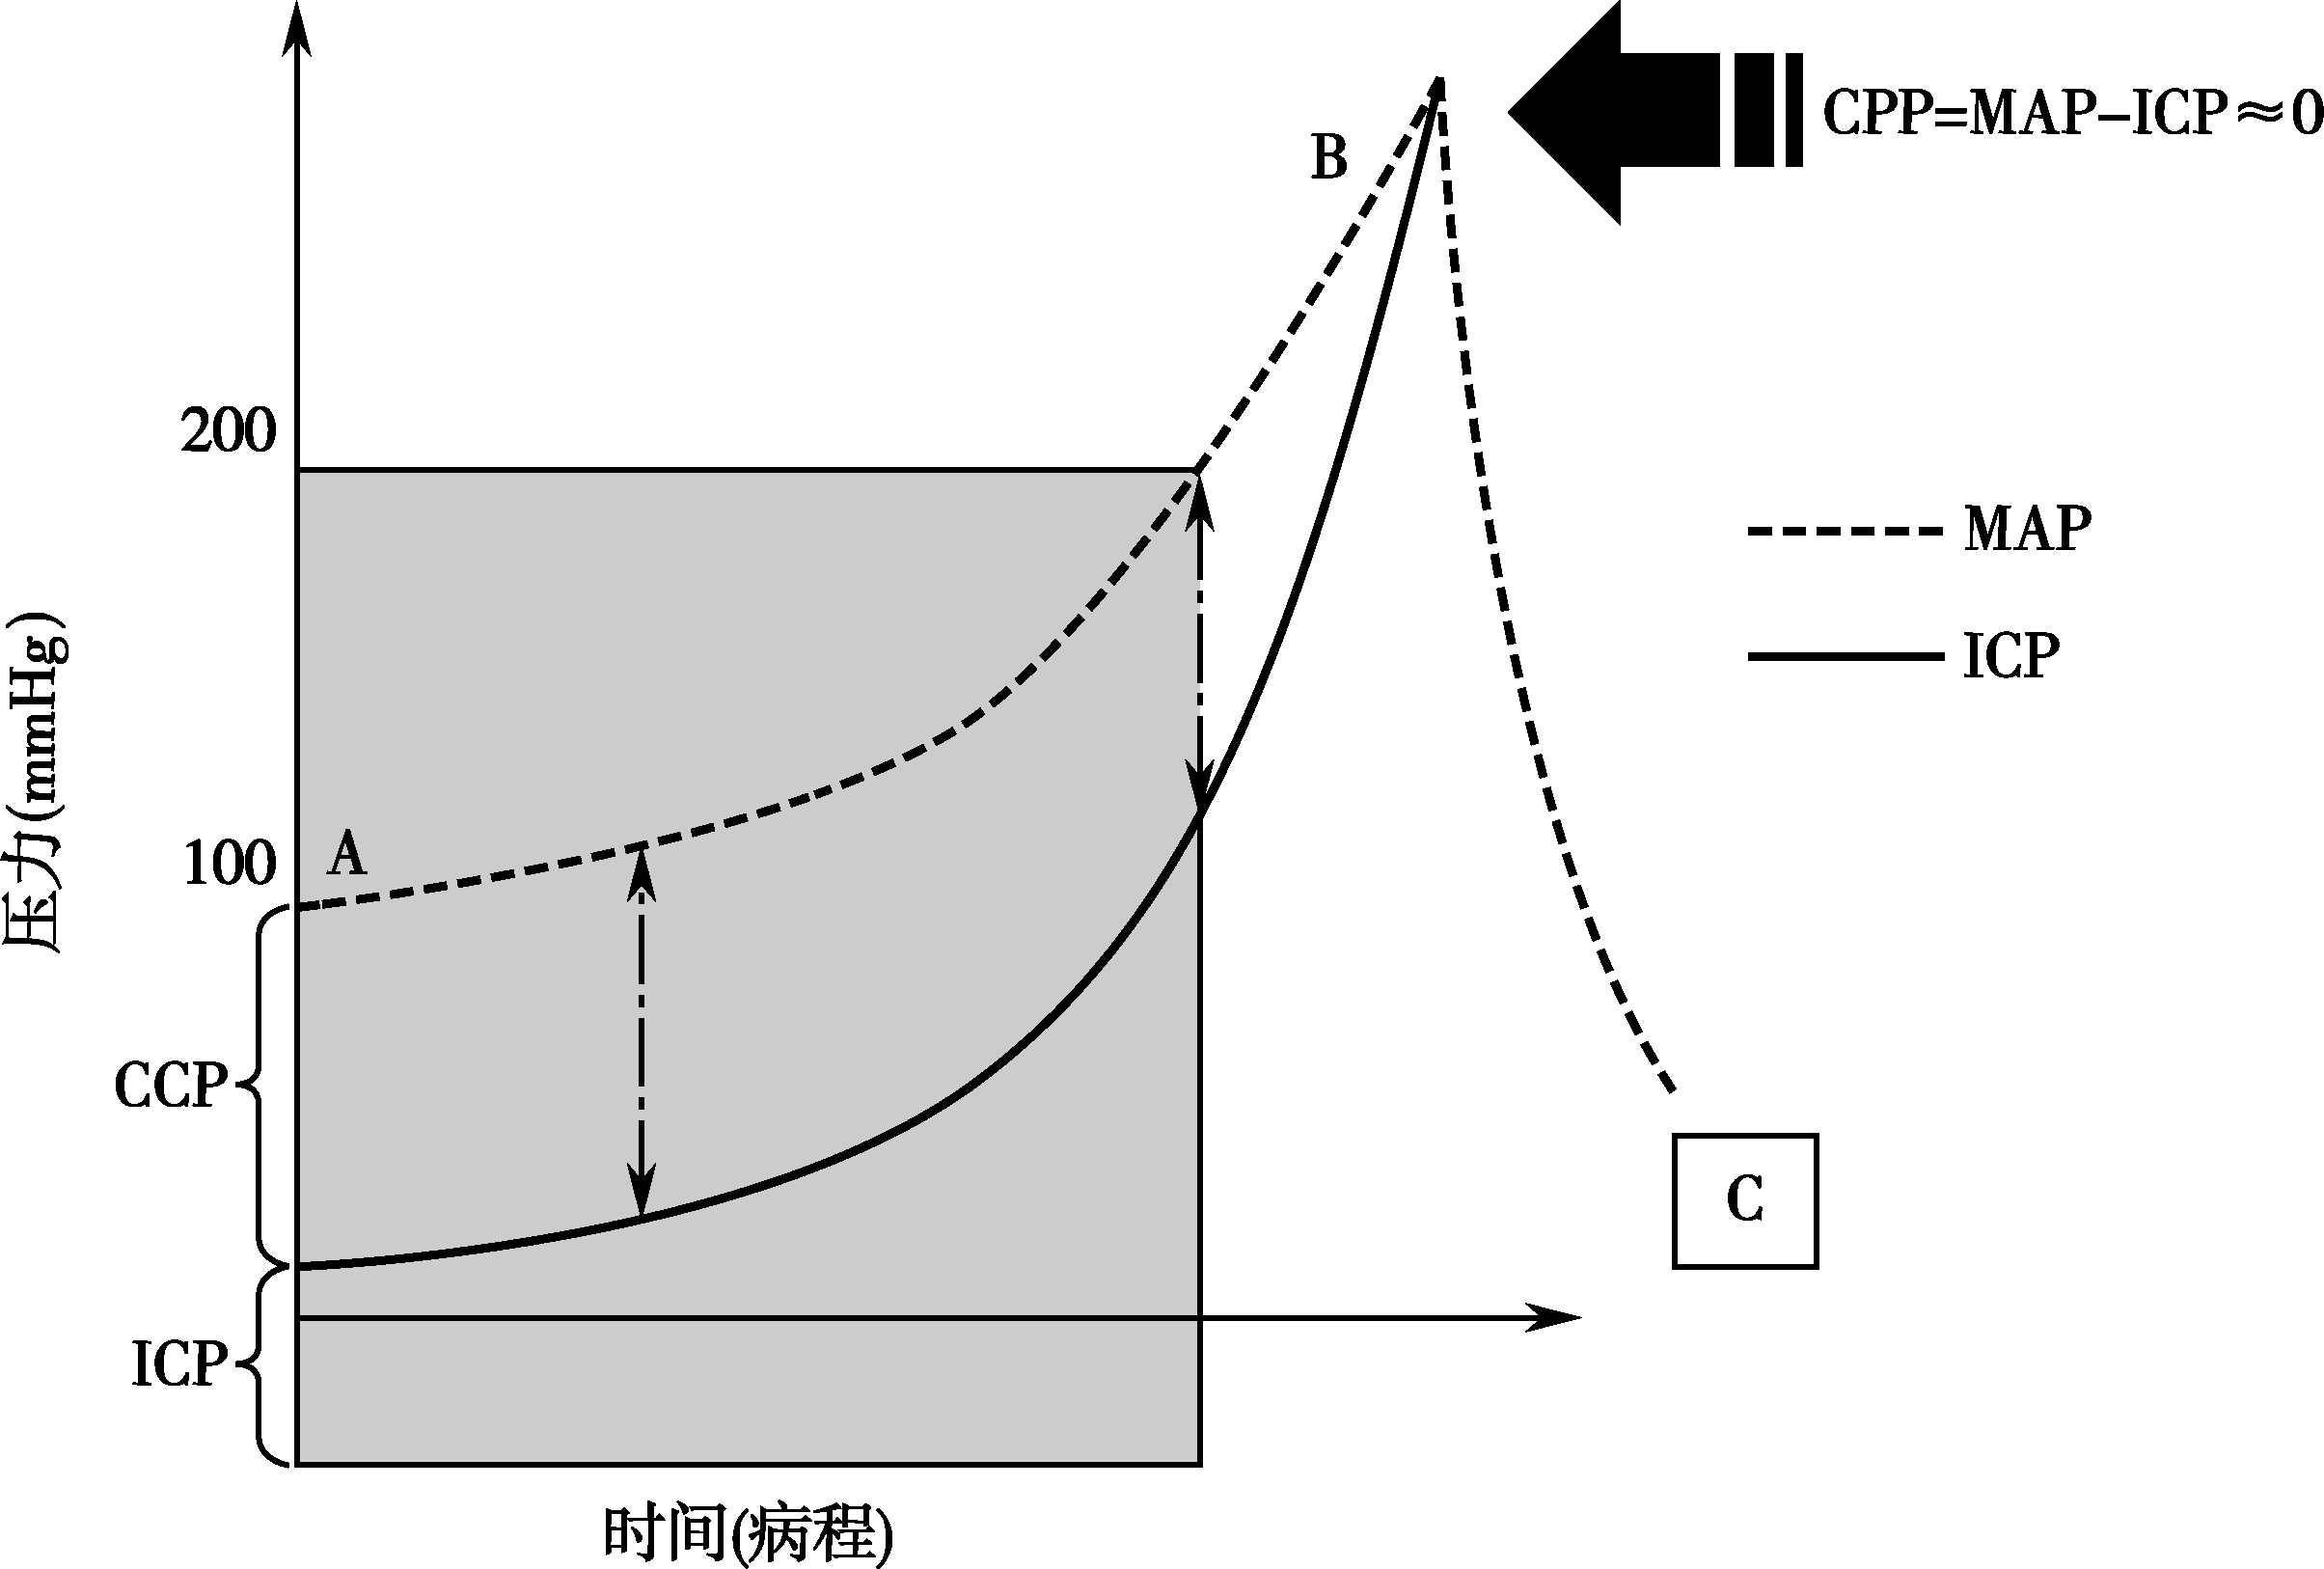
\includegraphics[width=4.01042in,height=2.70833in]{./images/Image00153.jpg}
 \captionsetup{justification=centering}
 \caption{Cushing反射示意图}
 \label{fig41-1}
  \end{figure} 

视神经鞘为脑蛛网膜的延续。视网膜中央动、静脉位于视神经鞘内与视神经伴随而行,在视神经乳头处出入眼底。当颅内压增高时,蛛网膜下腔内的压力增高,视神经鞘内压力也增高,而使网膜中央静脉回流受阻,静脉内压力增高。检眼镜检查可见视乳头隆起、边缘不清、颜色发红,眼底静脉迂曲、怒张。由于毛细血管扩张、出血,检查时可见到点、片状,甚至火焰状出血。早期或轻度的视神经乳头水肿,一般不影响视力,如颅高压持续存在或继续发展,可出现盲点扩大,中心视力暗点及阵发性黑矇,病情再进一步发展,发生继发性视神经萎缩,视力持续下降直至失明。视神经乳头水肿虽是颅内压增高的特征性体征,但并非所有病例均有。

\paragraph{展神经麻痹与复视}

因展神经在颅内行走较长,颅内压增高时容易因挤压及牵拉受伤而出现单侧或双侧不全麻痹,出现复视。此症状无定位意义。故又称为“假定位征”。

\paragraph{意识障碍}

反应迟钝、嗜睡、昏睡至昏迷的各种意识障碍均可发生。系与颅内压增高时脑干网状结构上行激活系统及广泛大脑皮质受损有关。

\paragraph{抽搐}

、去大脑强直发作 与颅内压增高时脑干受压、脑供血不足、脑膜受刺激等有关。

\paragraph{生命指征的改变}

血压增高、脉搏缓慢、呼吸慢而深等;随着颅内压增高,可出现瞳孔缩小、对光反射迟钝、或忽大忽小、边缘不整、变化多端。常预示脑疝即将发生,应立即采取抢救措施。

\paragraph{并发全身其他系统病变的临床表现}

①胃肠功能紊乱及消化道出血:部分颅内压增高的患者可表现胃肠功能的紊乱,出现呕吐,胃及十二指肠出血及溃疡和穿孔等。这与颅内压增高引起下丘脑自主神经中枢缺血而致功能紊乱有关。也有人认为颅内压增高时,消化道黏膜血管收缩造成缺血,因而产生广泛的消化道溃疡。②神经源性肺水肿:在急性颅内压增高患者中,发生率高达5\%~10\%。这是由于下丘脑、延髓受压导致α-肾上腺素能神经活性增高,血压反应性增高,左心负荷过重,左心房及肺静脉压增高,肺毛细血管压力增高,液体外渗,引起肺水肿,患者表现为呼吸急促,痰鸣,并有大量泡沫状血性痰液。

\paragraph{小儿颅内压增高的表现}

小儿因不会诉说头痛,常表现为烦躁、哭闹或脑性尖叫,频繁呕吐、抽搐以至去脑强直发作,意识丧失。查体可见囟门隆起、扩大,颅缝裂开,头围增大,以及头皮静脉怒张;额、顶、颞及枕部突出膨大呈圆形,颈部静脉充盈,对比之下颜面很小;严重颅内压增高,压迫眼球,形成双目下视,巩膜外露的特殊表情,称落日征。

\subsubsection{脑疝的表现}

各种原因引起的颅内压增高,都可导致脑组织向压力相对较低的部位移位,形成脑疝。脑疝一般是逐渐形成的,但遇剧烈呕吐、咳嗽或腰穿等情况时,颅内压可急剧升高或颅腔与椎管间的压力失去平衡,可导致脑疝的骤然发生或原有脑疝加重。因此,在临床上怀疑慢性颅内压增高是因颅内占位性病变所引起时,作腰椎穿刺应慎重或尽量不做,以免致脑疝;确因诊断需要检查脑脊液时,腰穿前应使用一次高渗性脱水剂,穿刺放脑脊液时尽量不要拔出针芯且放液量宜少,穿刺后去枕平卧,头低位,并继续用高渗性脱水剂治疗。颅内可发生脑疝的部位虽多,但并非所有脑疝均有临床意义。临床上常见而危害大的有小脑幕裂孔下疝、枕骨大孔疝和小脑幕裂孔上疝,它们可单独存在或合并发生。详见本书第25章“急性脑功能衰竭”。

\subsubsection{颅内压监测}

利用各种颅内压监测技术对颅内压进行检测,可直接获得颅内压的数据为颅内高压诊断提供最直接的依据。目前颅内压监测技术分为有创颅内压监测技术和无创颅内压监测技术。有创颅内压监测技术包括脑室内插管法、硬脑膜外传感器、光纤探头监测ICP和腰椎穿刺检测ICP。有创颅内压监测技术准确性好,特别是脑室内插管法被认为ICP检测的“金标准”。但其缺点是有创、易感染、技术要求高、耗材贵不易临床推广。无创颅内压监测技术其优点是无创、技术要求低、不会引起任何不良反应、无耗材消耗、可以反复进行监测。但其准确性一般,能达到90\%。

\subsubsection{诊断性治疗}

用脱水药物如20\%甘露醇等静注,如颅内压增高症状缓解,则有诊断价值。

\subsubsection{辅助检查}

电子计算机X线断层扫描(CT)、磁共振成像(MRI)、脑血管造影(DSA)、头颅X线摄片等既可辅助判断颅内压增高,也可帮助明确颅内压增高的病因。腰椎穿刺测量脑脊液的压力可直接判断颅内压的高低。

\subsubsection{颅内压增高的分类与分级}

根据颅内压增高的范围可分为:①弥漫性颅内压增高:在颅内各分腔间没有大的压力差,其耐受限度较高,很少引起脑疝,压力解除以后神经的恢复较快。如见于蛛网膜下腔出血、弥漫性脑膜炎、脑水肿等。②局灶性颅内压增高:压力先在病灶附近增高然后传递到颅内各处,在颅内各分腔之间有较明显的压力差,其耐压限度较低,常有明显的脑组织移位(脑疝),超过一定时间以后解除压力,受损的脑组织功能恢复较慢。区别这两类颅内压增高对于估计预后与决定治疗有重要意义。根据ICP的增高程度可以分为三级:压力在200~260mmH\textsubscript{2}
O者为轻度增高;261~520mmH\textsubscript{2}
O者为中度增高;超过520mmH\textsubscript{2} O者为严重增高。

\subsection{治疗}

对颅内压增高的患者,既要及时治疗原发病变,又要尽可能降低颅内压,及时中断恶性循环,防治脑疝。

\subsubsection{一般疗法}

包括:①卧床休息,密切观察生命体征;②抬高头部约15°~30°,以利颅内静脉回流;③吸氧,保持呼吸道通畅,昏迷患者不能排痰者,应考虑气管切开;④呕吐频繁者,应暂禁食,静脉补足液体和热量或改给全胃肠外营养;⑤限制水盐摄入量,静滴液量成人每日不超过1500~2000ml(不包括脱水剂量),其中电解质液不超过500ml;⑥防止受凉、咳嗽、避免激动、生气,保持大便通畅,防止便秘;⑦对症处理:如疼痛、呕吐者,给以镇静止吐药物;⑧有条件时可行颅内压监测,以利于指导用药。

\subsubsection{并发高血压的处理}

当颅内压增高到一定程度时脑血管自动调节功能就受损,主要靠全身性血管的加压反应来提高血压以提高脑灌注压维持脑部血流量。因此,颅内压增高的患者血压升高是机体的一个自我保护性反应,不必要强行将血压降得过低,以免降低脑灌注压加重脑损害。对此类患者血压应控制在什么水平及如何控制目前还缺乏统一标准。借鉴急性脑血管病高血压处理方法,提出如下建议:①收缩压<
220mmHg或舒张压<
120mmHg时应观察,除非其他终末器官受损,如主动脉夹层分离、急性心肌梗死、肺水肿或高血压脑病;②收缩压>
220mmHg或舒张压121~140mmHg时用拉贝洛尔10~20mg静注,1~2分钟,每10分钟可重复或加倍使用,最大剂量300mg;或者尼卡地平5mg/h静滴,每5分钟增加2.5mg/h,直至最大剂量15mg/h,直到达到预期效果;目标是使血压降低10\%~15\%;最好应用微量输液泵,避免血压降得过低。③如有ICP检测,CPP应保持在60~70mmHg以上。但必须强调,对于颅内压增高并发高血压的处理,应重点针对病因治疗,以便有效降低颅内压,血压会自动下调。

\subsubsection{脱水疗法}

脑水肿是构成颅内压增高的主要因素,控制脑水肿的发生与发展对降低颅内压极为重要。采用脱水药物是最常用的降低颅内压力的方法。当颅内占位性病变的晚期突然发生脑疝时,也常需先用脱水疗法,待症状缓解后,再行手术治疗。常用的脱水剂有下列几种:

\hypertarget{text00107.htmlux5cux23CHP4-6-3-3-1}{}
(一) 渗透性脱水剂

包括各种高渗性晶体及大分子药物。使用后由于血脑屏障的选择性作用,药物进入血液后不能迅速转入脑与脑脊液中,致使血液呈现高渗状态,造成血液与组织间渗透压差,促使组织间液、细胞内液及脑脊液内的水分转移至血液内;且高渗物质由肾小球滤出时,在近端肾小管中造成高渗透压而产生利尿作用;同时因血液的高渗透压反射性的抑制脉络丛的分泌,使脑脊液分泌减少,结果均致颅内压下降。但该类药物只有在脑血管功能正常时才能很好地发挥作用,脑血管损伤时其疗效受到影响。常用药物有:

\paragraph{甘露醇}

甘露醇是单糖,分子量为182,在体内不被代谢,为广泛应用的渗透性脱水剂。甘露醇对血糖没有影响,因此糖尿病患者也可以使用。其作用机制:首先是组织的脱水作用,在血管壁完整的情况下,通过提高血浆渗透压,导致脑组织内细胞外液、脑脊液等水分进入血管内。其次是利尿作用,通过增加血容量,促进前列腺素Ⅰ分泌,从而扩张肾血管,提高肾小球滤过率;另外由于甘露醇在肾小管重吸收率低,故可提高肾小管内液渗透浓度,主要减少远端肾小管对水、Na\textsuperscript{+}
和其他溶质等的重吸收,从而将过多水分排出体外。它尚有清除自由基、减少其对细胞脂膜的破坏作用。虽然甘露醇的脱水作用强,是临床最常使用的脱水药物,但目前对使用甘露醇的剂量、次数及疗程等仍无统一意见,甚至存在较大争议。已知1g甘露醇可带出12.5ml水分,尿钠排泄0.5g。正常血浆渗透压范围是280~310mOsm/L,甘露醇高渗脱水的最佳作用区间是310~330mOsm/L,当渗透压超过330mOsm/L时就会产生肾和神经组织损害。甘露醇每次总量不宜超过60g,每日总量不宜超过300g。甘露醇治疗脑水肿的用量很关键,用量过少起不到脱水降颅压的作用,剂量过大又会产生不良反应,其量效关系非常明确。一般情况下,颅内压较轻或控制较好者用药剂量相应减少,取有效量至最佳有效量之间即可;对于严重颅内高压,甚至脑疝抢救时,即使最佳有效剂量也往往不够理想,此时就应以抢救生命为重,须短期快速静脉注射20\%甘露醇250ml甚至500ml才能取得疗效,或者配合其他脱水药物一起使用。甘露醇的临床常用剂量为每次0.25~0.5g/kg,浓度为20\%,于30~40分钟静滴完,进入血管后10~20分钟开始起作用,半衰期为71.15分钟±
27.02分钟,2~3小时降颅压效果最强,可维持作用4~6小时,大部分4小时左右经肾脏排出,故临床上间隔4~6小时用药一次。Marshall等监测8例脑损伤患者的ICP发现,不同剂量甘露醇间隔同样时间(8小时),小剂量(0.25g/kg)与大剂量(1g/kg)治疗后ICP降低的程度没有差异。所以,甘露醇用量不宜过大,用药时间不宜过长,停药时应逐渐减量。1999年美国心脏协会(AHA)方案建议,20\%甘露醇的用法为每次0.25~0.5g/kg,4~6小时1次。甘露醇的反跳现象:甘露醇的脱水作用有赖于血脑屏障的完整性,当血脑屏障的通透性增高时,甘露醇就可以逐步通过血脑屏障聚积于脑组织间隙,这样当停止静脉输入一段时间后,血浆渗透压就可能暂时低于脑组织的渗透压,此时水分由血浆反流入脑组织,使脑组织的含水量再度增高,脑水肿加重,颅内压回升,即出现所谓反跳现象,因此要严格控制用药间隔时间。还有学者在研究中发现,渗透性脱水剂从脑脊液清除的速率低于从血中清除的速率,所以停药后甘露醇在脑脊液和血中的渗透压梯度会短暂逆转,反而导致ICP较治疗前增高,形成所谓反跳现象。最常见不良反应为电解质紊乱,其他尚有排尿困难、血栓性静脉炎、过敏反应、甘露醇肾病等。其中甘露醇肾病常于大剂量快速静脉滴注时发生,往往会引起急性肾衰,一旦发生,立即停用甘露醇,改用其他脱水剂。轻者早期可应用血管扩张剂或利尿剂,病情严重者应透析治疗。

\paragraph{甘油果糖}

甘油果糖(10\%甘油、5\%果糖、0.9\%氯化钠)的渗透压是人体血浆的7倍,经静脉输液后能提高血浆渗透压,在血浆和脑之间形成渗透梯度,使水从脑转移向血浆,从而使脑组织脱水,并使脑脊液的产生减少,降低颅内压,消除脑水肿。甘油果糖不增加肾脏负担,无肾脏损害作用。甘油果糖进入体内参与代谢,产生水和二氧化碳,同时每500ml可提供1339kJ(320千卡)的热量。通过血脑屏障进入脑组织,氧化成磷酸化基质,参与脑代谢并提供热量,增强脑细胞活力,使脑代谢改善。同时甘油果糖能有效地改善血液流变学状态,改善微循环,增加脑血流量及供氧量。甘油果糖单用降颅压起效慢,作用维持时间长,费用大。现在多主张将甘油果糖和甘露醇联合应用,既迅速降颅压,改善症状,又减轻肾脏负担,保护肾功能,降低费用支出,也克服了甘露醇的颅内压反跳现象。

\paragraph{甘油}

一些学者认为,甘油有增加脑血流,改善脑代谢和减轻脑水肿的作用。其作用温和而持久,没有反跳现象,不会导致电解质紊乱,适用于肾功能不全或长期未控制的老年高血压患者。但它起效较慢,多在用药1周后效果显著,且在快速滴注时会出现溶血作用,导致血红蛋白尿,故滴速应控制在30滴/分钟以下,与甘露醇联合应用效果较好。汇总分析也表明,它能降低卒中后14天内的死亡率,但不能降低1年内的死亡率。它可以口服或静脉注射。①口服法:口服剂量为1~2g/(kg•d),用生理盐水配成50\%的甘油盐水,每次30~50ml口服,每日3次。副作用为恶心、呕吐、腹胀。②注射法:用复方甘油注射液,其中含10\%甘油,90\%生理盐水,为一种长效脱水剂。成人每次500ml,以100~150ml/h速度静脉输入,每日1~2次。注射后2~4小时发挥作用,持续18小时。

\paragraph{高渗盐水}

用高渗盐水降颅内压是目前学者们研究的热点之一。研究表明,高渗盐水能有效地减轻脑水肿、降低颅内压,其疗效甚至更优于目前临床最为常用的甘露醇。《ASA/AHA2007自发性脑出血治疗指南》亦明确将高渗盐水和甘露醇同时作为推荐的降颅压药物(Ⅱa类,证据水平C)。纳入6个随机对照试验的系统评价结果表明,高渗盐水在降颅压幅度、起效时间、最大效应时间和维持时间上均优于甘露醇,且不降低颅内灌注压和不增加全身副作用的发生率。高渗盐水减轻脑水肿、降低颅内压比甘露醇更安全有效,是一种可供选用的脱水剂。高渗盐水降低颅内压,提高脑灌注压的机制可能与下列因素有关:①提高血浆渗透压,使组织间液、脑细胞内液进入血液中,从而减轻脑水肿、降低颅内压力;②使血管内皮细胞、红细胞脱水,增加脑血流量。但静脉注射高渗盐水可能会导致血浆渗透压过高、充血性心力衰竭、电解质紊乱、酸碱失衡、脑桥中央髓鞘破坏等副作用。下一步需要解决的问题是:①用高渗盐水降颅压的最佳用量与时机;②如何避免副作用的发生;③该药能否成为一线降颅压药物。

\paragraph{人体白蛋白}

它是通过提高血浆胶体渗透压使脑组织间液的水分进入循环血中,达到脱水降颅压的作用。提高胶体渗透压可较长时间保持完好的血流动力学及氧的输送,而且扩张血容量后,使抗利尿激素分泌减少而利尿,对血容量不足、低蛋白血症的颅内高压、脑水肿患者尤为适用。因其增加心脏负荷,有心功能不全者须慎用。血脑屏障严重破坏的病变,白蛋白能漏出至毛细血管而加剧颅内高压,使用时须注意。另外,白蛋白价格昂贵,患者很难承担其费用。

\hypertarget{text00107.htmlux5cux23CHP4-6-3-3-2}{}
(二) 利尿性脱水剂

本类药物抑制肾小管对 Na\textsuperscript{+} 、Cl\textsuperscript{−}
、K\textsuperscript{+}
的重吸收,使尿量显著增加,循环血量减少,组织水分逸出,造成机体脱水而间接地使脑组织脱水,降低颅内压。但单独应用则其降低颅内压作用较弱;若与渗透性脱水剂合用,则可加强降颅内压效果。常用利尿剂有:呋塞米每次20~40mg,每日2~4次肌注或静注;布美他尼(丁尿胺)每次0.5~1mg肌注或静注,必要时30分钟后重复使用一次。呋塞米主要用于协助高渗性脱水剂的降颅压作用,心功能或肾功能不全的患者中应用此药可减轻心脏负荷,促进物质排泄,还可减少甘露醇的用量,从而减轻对肾小管的损害。一般建议与甘露醇交替使用。Roberts等通过动物实验研究呋塞米与甘露醇应用的最佳顺序,发现应用甘露醇15分钟后再用呋塞米可产生最明显和最持久降低ICP的效果。

\hypertarget{text00107.htmlux5cux23CHP4-6-3-3-3}{}
(三) 脱水疗法的注意事项

包括:①渗透性脱水剂可使钠、钾、氯的排出量稍有增加,但因其排出的水量很大,血清中电解质可无明显的变化,甚至血液浓缩反有相对增高的现象。1~2次用药可不必补电解质,如应用的时间较长或次数较多,则应严密观察电解质的变化并给予适量的补充。但利尿性脱水剂如呋塞米与布美他尼则易致电解质紊乱,不宜长期、频繁使用。②对颅内压增高并心功能不全、肺水肿、急性肾功能衰竭少尿期,一般不宜应用渗透性脱水剂,因可在短时间内使血容量急剧增加而加重心力衰竭;此时,最适宜用利尿性脱水剂。③在脱水剂疗法中,正确地掌握维持出入量的平衡是十分重要的,若入量过多则达不到脱水目的;反之,则可致血容量不足甚至发生低血容量性休克。一般应限制液体入量在1500~2000ml/d之内,其中包括盐水500ml。

\subsubsection{肾上腺皮质激素}

其减轻脑水肿、降低颅内压之作用机制是多方面的:①改善血脑屏障功能,降低毛细血管通透性,减轻血管源性脑水肿;②改善细胞膜的功能,重建细胞内外钾、钠离子的正常分布,减轻细胞毒性脑水肿;③抗氧化作用,对抗自由基,防止细胞膜磷脂的自由基反应,维持细胞膜的正常功能(自由基可使细胞膜上的多价不饱和脂肪酸产生脂质过氧化反应而失去功能);④抑制垂体后叶抗利尿激素的分泌,同时还能增加肾血流量抑制醛固酮的分泌。在降低颅内压力的效果上不及渗透性脱水剂,然而,其作用持久、温和,与其合用,能提高降压效果,防止反跳。常用地塞米松20~40mg/d或氢化可的松200~600mg/d,分次静滴。应注意防治其以下副作用:①抑制机体免疫力易导致感染;②使糖耐量降低,血糖升高;③诱发上消化道出血。目前在是否主张使用肾上腺皮质激素降低颅内压方面尚无统一意见。建议根据具体病情,权衡利弊作出选择。

\subsubsection{病因治疗}

各种原因所致的颅内压增高,均应采取积极而有效的方法对其原发病进行治疗,才能阻断恶性循环,使各种对症治疗收到良效。如对颅内肿瘤、各种炎症、脑血管病等,均应针对不同病因给以相应治疗。

\subsubsection{其他治疗}

包括:①人工冬眠疗法。②人工过度换气:采用短期控制性过度换气,使呼吸加深加快,降低PaCO\textsubscript{2}
至32~35mmHg,可诱导脑血管收缩,导致颅内压下降,停止过度换气后其效果可维持数小时。尤其用于外伤性颅内高压。③亚低温治疗:临床试验已经证实对外伤性颅内高压的患者实施亚低温治疗(32~35℃)可有效降低颅内压,未发现明显的心律失常、凝血机制障碍和感染等并发症。④脑保护剂及脑细胞代谢活化剂的运用,如ATP、COA、细胞色素C、脑活素等,均可酌情选用。⑤高压氧疗法:适用于缺氧引起的脑水肿病例。

\subsubsection{颅高压危象的外科手术治疗}

临床上颅高压危象可导致脑疝形成。脑疝症状一旦出现,除立即经静脉快速滴注或推注脱水剂、以期望缓解症状外,还应依不同情况尽可能做手术处理。

\paragraph{急性脑室扩张}

急性脑室扩张多见于小脑出血或梗死向前推压第四脑室、蛛网膜下腔出血、脑实质出血破入蛛网膜下腔等情况。一旦出现急性脑室扩张颅内压会急剧升高。在药物治疗无效时,应急诊行侧脑室穿刺引流术。

\paragraph{小脑幕裂孔下疝}

若病因诊断明确,应立即开颅手术,切除病变以达到缓解颅内压增高的目的;对于未能明确诊断的病例,应作紧急颞肌下减压术,如情况许可并应将小脑幕裂孔边缘切开,促使脑疝的复位。

\paragraph{枕骨大孔疝}

应紧急作脑室穿刺,缓慢放出脑室液,使颅内压慢慢下降,然后施行脑室持续引流术。待脑疝症状缓解后,对颅后凹开颅术,切除原发病变,对脑积水病例施行脑脊液分流术。
\protect\hypertarget{text00108.html}{}{}

\chapter{高血压危象}

在急诊工作中,常常会遇到一些血压突然和显著升高的患者,伴有症状或有心、脑、肾等靶器官的急性损害,如不立即进行降压治疗,将产生严重并发症或危及患者生命,称为高血压危象(hypertensive
crisis)。其发病率约占高血压患者的1\%~5\%左右。

有关高血压患者血压急速升高的术语有:高血压急症、高血压危象、高血压脑病、恶性高血压、急进型高血压等。美国高血压预防、检测、评价和治疗的全国联合委员会第七次报告(JNC7)对高血压急症(hypertensive
emergencies)和次急症(hypertensive
urgencies)的定义简单明了。高血压急症是以伴有即将发生或进展的靶器官功能障碍为特征的血压急剧升高(通常超过180/120mmHg),为防止或限制靶器官的受损,需要迅速降低血压(可以不达到正常范围)。如果仅有血压显著升高,但不伴靶器官新近或急性功能损害,则定义为高血压次急症。广义的高血压危象包括高血压急症和次急症;狭义的高血压危象等同于高血压急症。

高血压急症主要包括:①急性脑血管病:脑出血、脑动脉血栓形成、脑栓塞、蛛网膜下腔出血等。②主动脉夹层动脉瘤。③急性左心衰竭伴肺水肿。④急性冠状动脉综合征(不稳定心绞痛、急性心肌梗死)。⑤子痫前期、子痫。⑥急性肾功能衰竭。⑦微血管病性溶血性贫血。

高血压次急症主要包括:①高血压病3级(极高危)。②嗜铬细胞瘤。③降压药物骤停综合征。④严重烧伤性高血压。⑤神经源性高血压。⑥药物性高血压。⑦围术期高血压。

高血压急症与高血压次急症均可合并慢性器官损害,区别两者的唯一标准是有无新近发生的或急性进行性的严重靶器官损害。高血压水平的绝对值不构成区别两者的标准,因为血压水平的高低与是否伴有急性靶器官损害或损害的程度并非成正比。

高血压急症是一种严重危及生命的临床综合征,特别强调了心、脑、肾等重要靶器官的功能问题。在高血压急症治疗中,“降低血压”只是一种治疗手段,“保护或恢复靶器官的功能”才是“目的”。近年来,随着对自动调节阈的理解,临床上得以能够正确的把握高血压急症的降压幅度。尽管血压有显著的可变性,但血压的自动调节功能可维持流向生命器官(脑、心、肾)的血流在很小的范围内波动。例如,当平均动脉压(MAP)低到60mmHg或高达120mmHg,脑血流量可被调节在正常压力范围内。然而,在慢性高血压患者,其自动调节的下限可以上升到MAP
的100~120mmHg,高限可达150~160mmHg,这个范围称为自动调节阈。达到自动调节阈低限时发生低灌注,达到高限则发生高灌注。与慢性高血压类似,老年患者和伴有脑血管疾病的患者自动调节功能也受到损害,其自动调节阈的平均低限大约比休息时MAP低20\%~25\%。对高血压急症患者最初的治疗可以将MAP谨慎地下降20\%的建议就是由此而来。

\subsection{病因与发病机制}

\subsubsection{病因}

高血压危象的促发因素很多,最常见的是在长期原发性高血压患者中血压突然升高,约占40\%~70\%。另外,25\%~55\%的高血压危象患者有可查明原因的继发性高血压,肾实质病变占其中的80\%。高血压危象的继发性原因主要包括:①肾实质病变:原发性肾小球肾炎、慢性肾盂肾炎、间质性肾炎。②涉及肾脏的全身系统疾病:系统性红斑狼疮、系统性硬皮病、血管炎。③肾血管病:结节性多动脉炎、肾动脉粥样硬化。④内分泌疾病:嗜铬细胞瘤、库欣综合征、原发性醛固酮增多症。⑤药品:可卡因、苯异丙胺、环孢素、可乐定撤除、苯环利定。⑥主动脉狭窄。⑦子痫和子痫前期。

\subsubsection{发病机制}

各种高血压危象的发病机制不尽相同,某些机制尚未完全阐明,但与下列因素有关。

\paragraph{交感神经张力亢进和缩血管活性物质增加}

在各种应激因素作用下,交感神经张力、血液中血管收缩活性物质(如肾素、血管紧张素Ⅱ等)大量增加,诱发短期内血压急剧升高。

\paragraph{局部或全身小动脉痉挛}

①脑及脑细小动脉持久性或强烈痉挛导致脑血管继之发生“强迫性”扩张,结果脑血管过度灌注,毛细血管通透性增加,引起脑水肿和颅内高压,诱发高血压脑病。②冠状动脉持久性或强烈痉挛导致心肌明显缺血、损伤甚至坏死等,诱发急性冠脉综合征。③肾动脉持久性或强烈收缩导致肾脏缺血性改变、肾小球内高压力等,诱发肾功能衰竭。④视网膜动脉持久性或强烈痉挛导致视网膜内层组织变性坏死和血-视网膜屏障破裂,诱发视网膜出血、渗出和视神经乳头水肿。⑤全身小动脉痉挛导致压力性多尿和循环血容量减少,反射性引起缩血管活性物质进一步增加,形成病理性恶性循环,加剧血管内膜损伤和血小板聚集,最终诱发心、脑、肾等重要脏器缺血和高血压危象。

\paragraph{脑动脉粥样硬化}

高血压促成脑动脉粥样硬化后斑块或血栓破碎脱落易形成栓子,微血管瘤形成后易于破裂,斑块和(或)表面血栓形成增大,最终致动脉闭塞。在血压增高、血流改变、颈椎压迫、心律不齐等因素作用下易发生急性脑血管病。

\paragraph{其他}

引起高血压危象的其他相关因素尚有神经反射异常(如神经源性高血压危象等)、内分泌激素水平异常(如嗜铬细胞瘤高血压危象等)、心血管受体功能异常(如降压药物骤停综合征等)、细胞膜离子转移功能异常(如烧伤后高血压危象等)、肾素-血管紧张素-醛固酮系统的过度激活(如高血压伴急性肺水肿等)。此外,内源性生物活性肽、血浆敏感因子(如甲状旁腺高血压因子、红细胞高血压因子等)、胰岛素抵抗、一氧化氮合成和释放不足、原癌基因表达增加以及遗传性升压因子等均在引起高血压急症中起一定作用。

\subsection{诊断}

接诊严重的高血压患者后,病史询问和体格检查应简单而有重点,目的是尽快鉴别高血压急症和次急症。应询问高血压病史、用药情况、有无其他心脑血管疾病或肾脏疾病史等。除测量血压外,应仔细检查心血管系统、眼底和神经系统,了解靶器官损害程度,评估有无继发性高血压。如果怀疑继发性高血压,应在治疗开始前留取血和尿液标本。实验室检查至少应包括心电图和尿常规。高血压急症的临床特征见表\ref{tab42-1}。

\begin{table}[htbp]
\centering
\caption{高血压急症患者的临床特征}
\label{tab42-1}
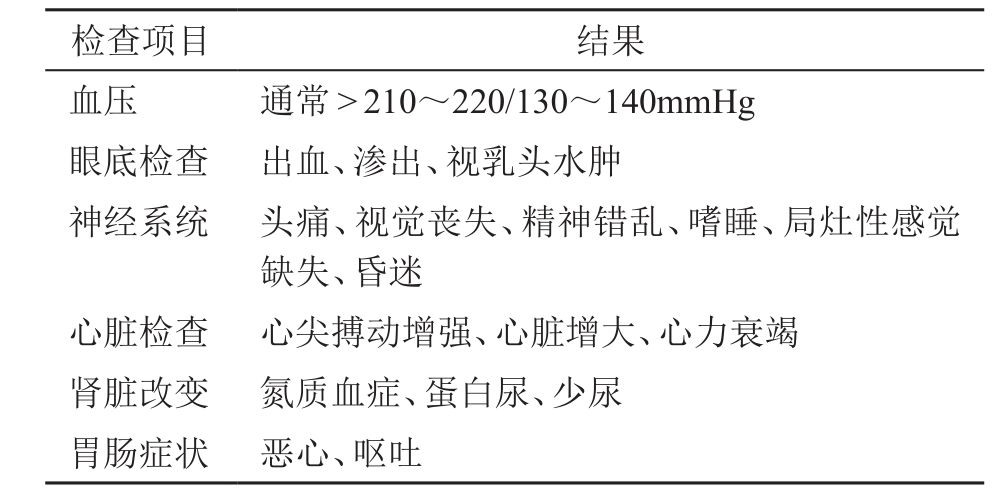
\includegraphics[width=3.29167in,height=1.625in]{./images/Image00154.jpg}
\end{table}

高血压急症患者通常血压很高,收缩压> 210mmHg或舒张压>
140mmHg。但是,鉴别诊断的关键因素通常是靶器官损害,而不是血压水平。妊娠妇女或既往血压正常者血压突然增高、伴有急性靶器官损害时,即使血压测量值没有达到上述水平,仍应视为高血压急症。

单纯血压很高、没有症状也没有靶器官急性或进行性损害证据的慢性高血压患者(其中可能有一部分为假性高血压患者),以及因为疼痛、紧张、焦虑等因素导致血压进一步增高的慢性高血压患者,通常不需要按高血压急症处理。

\subsection{治疗}

\subsubsection{治疗原则}

治疗的选择应根据对患者的综合评价诊断而定,靶器官的损害程度决定血压下降到何种安全水平以限制靶器官的损害。治疗评价依据见表\ref{tab42-2}。

高血压急症应住院治疗,重症收入CCU(ICU)病房。酌情使用有效的镇静药以消除患者恐惧心理。在严密监测血压、尿量和生命体征的情况下,视临床情况的不同,应用短效静脉降压药物。定期采血监测内环境情况,注意水、电解质、酸碱平衡情况,肝、肾功能,有无糖尿病,心肌酶是否增高等,计算单位时间的出入量。降压过程中应严密观察靶器官功能状况,如神经系统的症状和体征,胸痛是否加重等。勤测血压(每隔15~30分钟),如仍然高于180/120mmHg,应同时口服降压药物。

降压目标不是使血压正常,而是渐进地将血压调控至不太高的水平,最大程度地防止或减轻心、脑、肾等靶器官损害。在正常情况下,尽管血压经常波动(MAP
60~150mmHg),但心、脑、肾的动脉血流能够保持相对恒定。慢性血压升高时,这种自动调节作用仍然存在。但调节范围上移,血压对血流的曲线右移,以便耐受较高水平的血压,维持各脏器的血流。当血压上升超过自动调节阈值之上时,便发生器官损伤。阈值的调节对治疗非常有用。突然的血压下降,会导致器官灌注不足。在高血压危象中,这种突然的血压下降,在病理上会导致脑水肿以及中小动脉的急慢性炎症甚至坏死。患者会出现急性肾衰、心肌缺血及脑血管事件,对患者有害无益。对正常血压者和无并发症的高血压患者的脑血流的研究显示,脑血流自动调节的下限大约比休息时MAP低20\%~25\%。因此初始阶段(几分钟到两个小时内)MAP的降低幅度不应超过治疗前水平的20\%~25\%。假如患者能很好耐受,且病情稳定,超过24小时后再把血压降至正常。无明显靶器官损害患者应在24~48小时内将血压降至目标值。

\begin{table}[htbp]
\centering
\caption{治疗评价的依据}
\label{tab42-2}
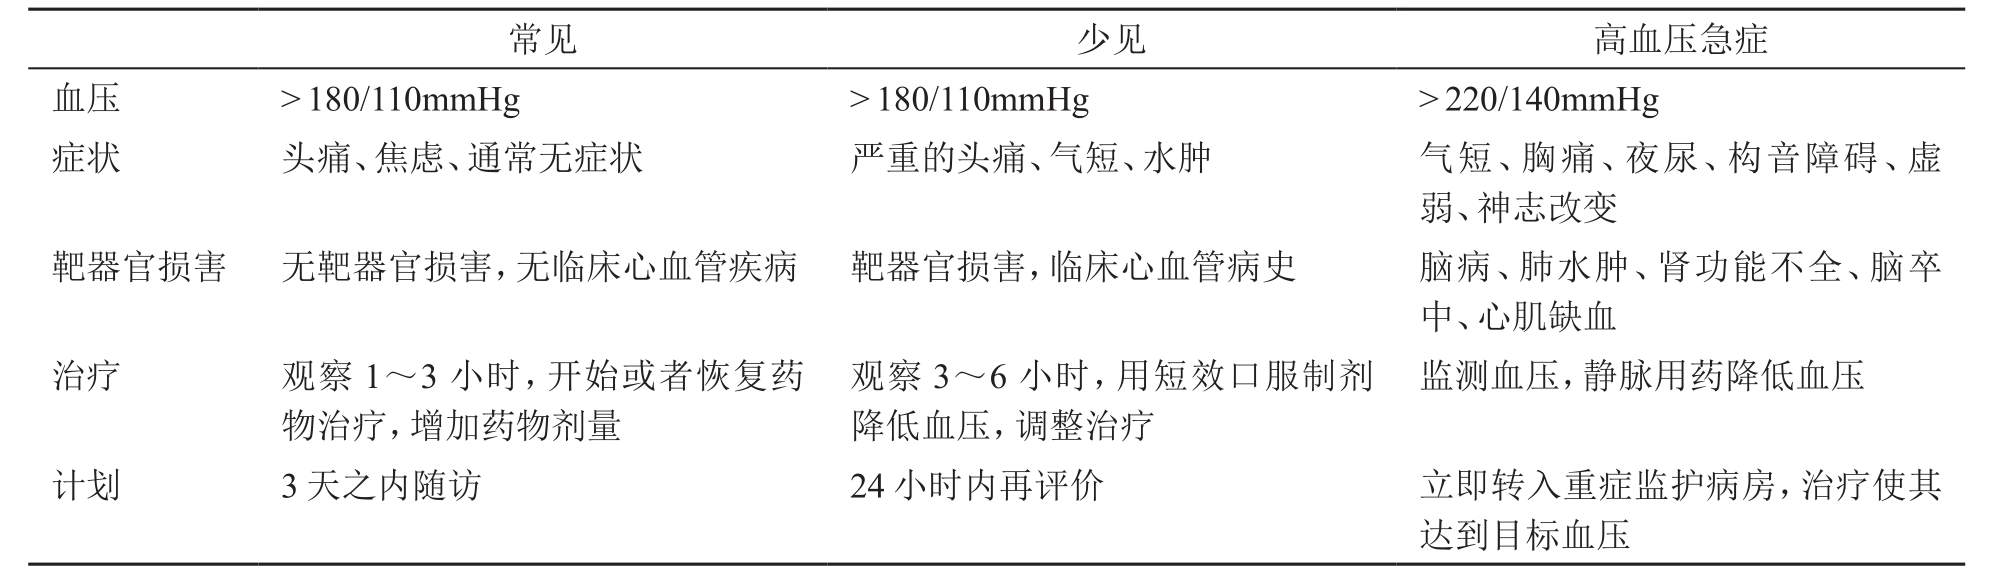
\includegraphics[width=6.64583in,height=1.91667in]{./images/Image00155.jpg}
\end{table}

上述原则不适用于急性缺血性脑卒中的患者。因为这些患者的颅内压增高、小动脉收缩、脑血流量减少,此时机体需要依靠MAP的增高来维持脑的血液灌注。此时若进行降压治疗、特别是降压过度时,可导致脑灌注不足,甚至引起脑梗死。因此一般不主张对急性脑卒中患者采用积极的降压治疗。关于急性出血性脑卒中合并严重高血压的治疗方案目前仍有争论,一般认为MAP
> 130mmHg时应该使用经静脉降压药物。

高血压次急症不伴有严重的靶器官损害,不需要特别的处理,可以口服抗高血压药物而不需要住院治疗。

高血压急症在临床上表现形式不同,治疗的药物和处理方法也有差异。高血压急症伴有心肌缺血、心肌梗死、肺水肿时,如果血压持续升高,可导致左室壁张力增加,左室舒张末容积增加,射血分数降低,同时心肌耗氧量增加。此时宜选用迅速降低血压,血压的目标值是使其收缩压下降10\%~15\%。此外,开通病变血管也是非常重要的。

高血压急症伴有神经系统急症是最难处理的。高血压脑病是排除性诊断,需排除出血性和缺血性脑卒中及蛛网膜下腔出血。以上各种情况的处理是不同的。①脑出血:在脑出血急性期,如果收缩压大于210mmHg,舒张压大于110mmHg时方可考虑应用降压药物,但要避免血压下降幅度过大,一般降低幅度为用药前血压20\%~30\%为宜,同时应脱水治疗降低颅内压。②缺血性脑卒中:一般当舒张压大于130mmHg时,方可小心将血压降至110mmHg。③蛛网膜下腔出血:首选降压药物以不影响患者意识和脑血流灌注为原则,蛛网膜下腔出血首期降压目标值在25\%以内,对于平时血压正常的患者维持收缩压在130~160mmHg之间。④高血压脑病:高血压脑病的血压值要比急性缺血性脑卒中要低。高血压脑病MAP在2~3小时内降低20\%~30\%。

高血压急症伴肾脏损害是非常常见的。有的患者尽管血压很低,但伴随着血压的升高,肾脏的损害也存在。尿中出现蛋白、红细胞、血尿素氮和肌酐升高,都具有诊断意义。高血压急症伴肾脏损害要在1~12小时内使MAP下降10\%~25\%,MAP在第1小时下降10\%,紧接2小时下降10\%~15\%。

高血压急症伴主动脉夹层有特殊处理。高血压是急性主动脉夹层形成的重要易患因素,因而降压治疗必须迅速实施,以防止主动脉夹层的进一步扩展。治疗时,在保证脏器足够灌注的前提下,应使血压维持在尽可能低的水平。首选静脉给药的β阻滞剂如艾司洛尔或美托洛尔,它可以减少夹层的发展。高血压伴主动脉夹层首期降压目标值将血压降至理想水平,在30分钟内使收缩压低于120mmHg。药物治疗只是暂时的,最终需要外科手术。

儿茶酚胺诱发的高血压危象,此症的特点是β肾上腺素张力突然升高。这类患者通常由于突然撤掉抗高血压药物造成。由于儿茶酚胺升高导致的高血压急症,最好用α受体阻滞剂,如酚妥拉明,其次要加用β受体阻滞剂。

怀孕期间的高血压急症,处理起来要非常谨慎和小心。硫酸镁、甲基多巴及肼屈嗪是比较好的选择。妊娠高血压综合征伴子痫前期使收缩压低于90mmHg。

围术期高血压处理的关键是要判断产生血压高的原因并去除诱因,去除诱因后血压仍高者,要降压处理。围术期的高血压的原因,是由于原发性高血压、焦虑和紧张、手术刺激、气管导管拔管、创口的疼痛等造成。手术前,降压药物应维持到手术前1天或手术日晨,长效制剂降压药宜改成短效制剂,以便麻醉管理。对于术前血压高的患者,麻醉前含服硝酸甘油、硝苯地平,也可用艾司洛尔300~500μg/kg静注,随后25~100μg/(kg•min)静点,或者用乌拉地尔(压宁定)首剂12.5~25mg,3~5分钟,随后5~40mg/h静点。拔管前用压宁定或艾司洛尔,剂量同前。

\subsubsection{降压药物的选择}

\hypertarget{text00108.htmlux5cux23CHP4-7-3-2-1}{}
(一) 急诊用药标准的考量

\paragraph{起效时间}

高血压急症急诊用药考虑的第一个因素是起效快。在常用降压药中,硝普钠起效最快,静注后“立即”起效;艾司洛尔和酚妥拉明起效时间为1~2分钟;硝酸甘油在5分钟内起效;拉贝洛尔和尼卡地平在5~10分钟起效;乌拉地尔稍慢,15分钟起效。从起效时间角度来衡量,除硝普钠起效最快,乌拉地尔起效稍慢外,上述所有药物都应符合高血压急症紧急降压的要求。

\paragraph{持续时间}

高血压急症急诊用药考虑的第二个因素是药物持续时间。其中持续时间较短的有:硝普钠(1~2分钟)、酚妥拉明(3~10分钟)、硝酸甘油(5~10分钟);居中的有:艾司洛尔(10~20分钟)、尼卡地平(1~4小时);较长的有:乌拉地尔(2~8小时)、拉贝洛尔(4~8小时)。药物持续时间主要与其半衰期有关。如药物持续时间很短,降压作用的平稳性就会很差,血压容易大起大落,需密切观察,随时调整药物的剂量和用药速度。临床上使用这类药物,比较麻烦,需密切监护,不太适合于急诊科使用。如药物持续时间较长,虽然降压作用的平稳性很好,但是一旦用药剂量过大,血压就会持续在较低水平,药物减量后需较长时间的等待,才能逐渐恢复,临床使用也不方便。故药物持续时间居中的降压药物,艾司洛尔和尼卡地平,有一定的优势。

\paragraph{常见且严重的不良反应}

药物的常见且严重的不良反应,主要决定于药物本身的特性。如β受体阻断药物艾司洛尔和拉贝洛尔,通过阻断心脏β受体,具有抑制心肌收缩力和减慢心率的作用。如果β\textsubscript{1}
受体阻断的选择性不强,还会有β\textsubscript{2}
受体阻断作用,使支气管收缩。钙离子拮抗剂中地尔硫{}
,也具有抑制心肌收缩力和减慢心率的作用。这些几乎是必然发生,和可能会很严重的不良反应,是临床医生选择药物时,常常不能容忍的问题,故只适用于高血压急症治疗中的一些特殊情况。

\hypertarget{text00108.htmlux5cux23CHP4-7-3-2-2}{}
(二) 高血压急症静脉降压药物

根据作用机制 ,经静脉降压药物主要分成以下几类:表\ref{tab42-3}。

\paragraph{血管扩张剂}

\hypertarget{text00108.htmlux5cux23CHP4-7-3-2-2-1-1}{}
(1) 硝普钠(sodium nitroprusside):

是一种起效快、持续时间短的强效静脉用降压药。静脉滴注数秒内起效,作用持续仅1~2分钟,血浆半衰期3~4分钟,停止注射后血压在1~10分钟内迅速回到治疗前水平。起始剂量0.25μg/(kg•min),其后每隔5分钟增加一定剂量,直至达到血压目标值。可用剂量0.25~10μg/(kg•min)。硝普钠应慎用或禁用于下列情况:①高血压脑病、脑出血、蛛网膜下腔出血。因该药可通过血-脑脊液屏障使颅内压进一步增高,影响脑血流灌注,加剧上述病情,故有颅内高压者一般不予应用。②急进型恶性高血压、高血压伴急性肾功能衰竭、肾移植性高血压、高血压急症伴严重肝功能损害等,因该药在体内与巯基结合后分解为氰化物与一氧化氮,氰化物被肝脏代谢为硫氰酸盐,全部需经肾脏排出。一般肾功能正常者硫氰酸盐排泄时间约为3天。故肝、肾功能不良患者易发生氰化物或硫氰酸盐中毒,产生呼吸困难、肌痉挛、精神变态、癫痫发作、昏迷、甚至呼吸停止等严重反应。③甲状腺功能减退和孕妇:因硫氰酸盐可抑制甲状腺对碘的摄取,加重甲状腺功能减退,且可通过胎盘诱发胎儿硫氰酸盐中毒和酸中毒。

\begin{table}[htbp]
\centering
\caption{治疗高血压急症的经静脉降压药物}
\label{tab42-3}
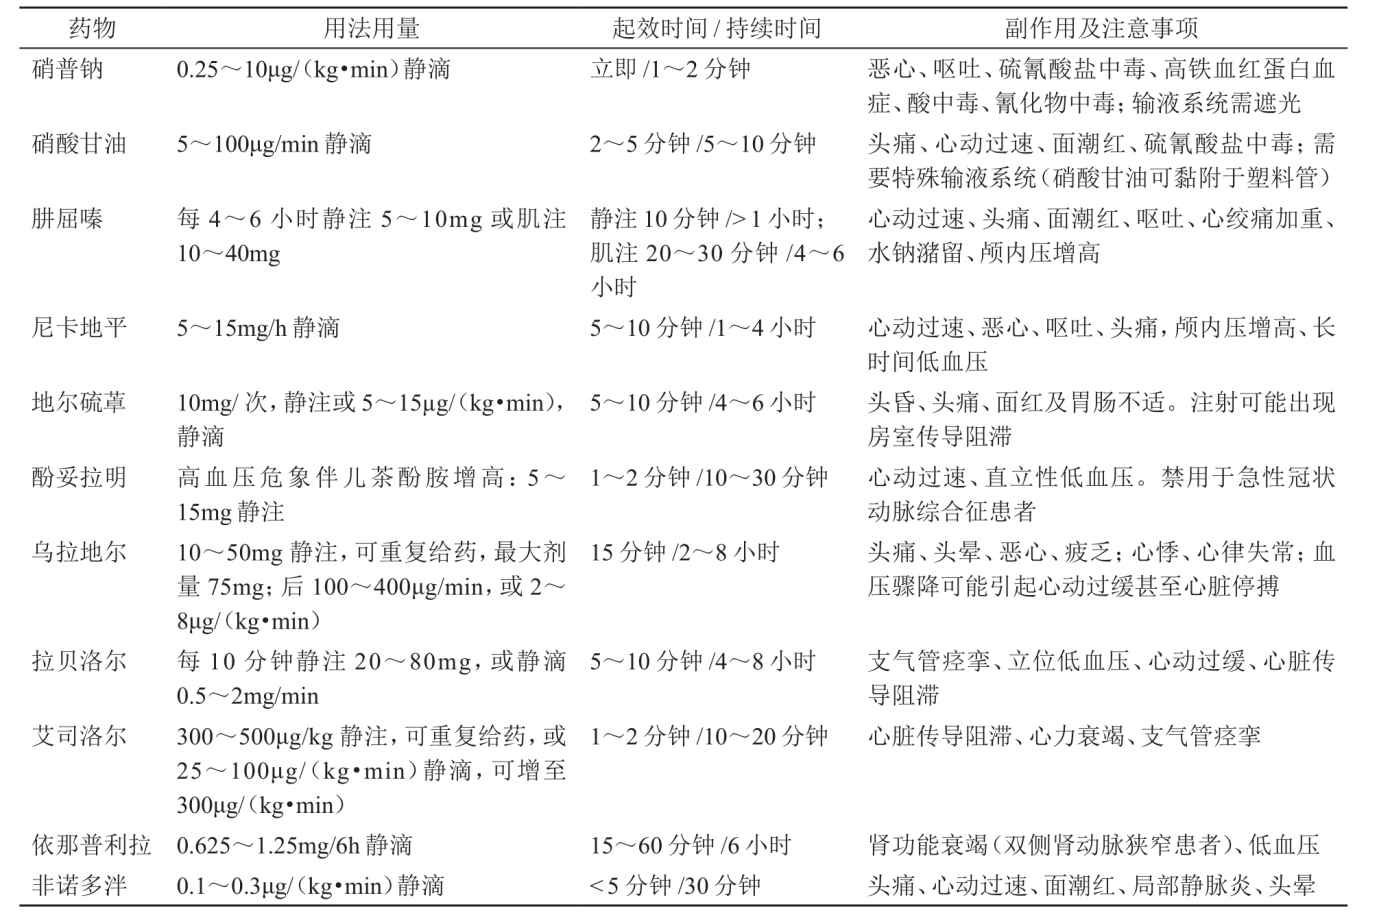
\includegraphics[width=6.69792in,height=4.47917in]{./images/Image00157.jpg}
\end{table}

过去认为硝普钠是高血压急症伴急性肺水肿、严重心功能衰竭、主动脉夹层的首选药物之一。其长期大剂量使用或患者存在肝、肾功能不全时,易发生氰化物中毒。故通常在初步控制病情后,应迅速改用其他药物。目前多数学者认为,由于硝普钠的严重副作用,它只用于无法获取其他降压药物时,和主动脉夹层等特殊情况,且患者的肝、肾功能正常的情况下;疗程尽可能短,输注速度应控制在2µg/(kg•min)以内,如大于4~10µg/(kg•min),必须同时给予解毒药物硫代硫酸盐。

\hypertarget{text00108.htmlux5cux23CHP4-7-3-2-2-1-2}{}
(2) 硝酸甘油(nitroglycerin):

能扩张静脉、动脉和侧支冠状动脉,特别适用于伴有中度血压增高的急性冠状动脉综合征或心肌缺血的患者。硝酸甘油起效快、消失也快,应注意监测静脉滴注的速率。该药小剂量时主要扩张静脉血管、较大剂量才能扩张小动脉,故可能需要每3~5分钟调快滴速,直到取得预期的降压效果。硝酸甘油静脉滴注2~5分钟起效,停止用药作用持续时间5~10分钟,可用剂量5~100µg/min。副作用有头痛、恶心呕吐、心动过速等。由于硝酸甘油是有效的扩静脉药物,只有在大剂量时才有扩动脉作用,能引起低血压和反射性心动过速,在脑、肾灌注存在损害时,静脉使用硝酸甘油可能有害。

\hypertarget{text00108.htmlux5cux23CHP4-7-3-2-2-1-3}{}
(3) 肼屈嗪(hydralazine):

通过直接舒张血管平滑肌降低血压。静脉注射每次10~20mg,10~15分钟起效,肌肉注射每次10~50mg,20~30分钟起效,血压持续下降可达12小时。虽然肼屈嗪循环半衰期只有3小时,但其效果减半的时间却达到了100小时,可能原因是肼屈嗪与肌性动脉壁长久结合。

由于肼屈嗪降压的效果持续和难于预测,不能控制其降压的强度,同时其会反射性引起每搏输出量和心率的增加,诱发或加重心肌缺血,应尽量避免在高血压急症时使用,仅用于子痫和惊厥患者。

\paragraph{钙拮抗剂}

\hypertarget{text00108.htmlux5cux23CHP4-7-3-2-2-2-1}{}
(1) 尼卡地平(nicardipine):

二氢吡啶类钙拮抗剂,通过抑制钙离子内流而发挥血管扩张作用。盐酸尼卡地平对血管平滑肌的作用比对心肌的作用强3万倍,其血管选择性明显高于其他钙拮抗剂。其扩张外周血管作用与硝苯地平相近,对冠脉的扩张比对外周血管更强。心脏抑制作用是硝苯地平的1/10,对心肌及传导系统无抑制作用。本品使心脏射血分数及心排血量增多,而左室舒张末压改变不多。能降低心肌耗氧量及总外周阻力,也可增加冠脉侧支循环,使冠状血流增加。5~15mg/h,缓慢静滴,直到出现预期反应。每5分钟可增加剂量2.5mg/h,最大剂量15mg/h。健康男性成年人,按0.01~0.02mg/kg盐酸尼卡地平静脉给予后,消除半衰期为50~63分钟。

尼卡地平与其他多数降压药物不同,在降低血压的同时,能增加重要器官的血流量,这是该药的重要特点之一。研究发现,尼卡地平可引起剂量依赖性的动脉血流量增加,程度为椎动脉>冠状动脉>股动脉>肾动脉。这是由于尼卡地平对椎-基底动脉及冠状动脉的选择性最高,这一特点不同于其他钙离子拮抗剂(如氨氯地平、非洛地平等就主要作用于周围血管),也有别于其他大多数降压药物。尼卡地平在降压的同时,可以改善脑、心、肾等重要器官的血流量,有效保护重要靶器官;故从保护靶器官角度考虑,尼卡地平可能是高血压急症治疗最佳的选择。

\hypertarget{text00108.htmlux5cux23CHP4-7-3-2-2-2-2}{}
(2) 地尔硫{} (diltiazem):

非二氢吡啶类钙拮抗剂,通过抑制钙离子向末梢血管、冠脉血管平滑肌细胞及房室结细胞内流,而达到扩张血管及延长房室结传导的作用。犬大剂量静脉注射盐酸地尔硫{}
可出现明显的心动过缓和房室传导改变。在犬和大鼠的亚急性和慢性毒性研究中,大剂量口服盐酸地尔硫{}
可引起肝脏损害。用法:10mg/次,静注或5~15µg(/kg•min)静滴。禁忌证主要为:①严重低血压或心源性休克患者。②Ⅱ度和Ⅲ度房室传导阻滞或病窦综合征(持续窦性心动过缓、窦性停搏和窦房阻滞等)。③严重充血性心衰患者。④严重心肌病患者。⑤对药物中任一成分过敏者。⑥妊娠或可能妊娠的妇女。⑦静脉给予盐酸地尔硫{}
和静脉给予β阻滞剂应避免在同时或相近的时间内给予(几小时内)。⑧室性心动过速患者,宽QRS心动过速患者(QRS≥0.12秒)使用钙通道阻滞剂可能会出现血流动力学恶化和室颤。静脉注射地尔硫{}
前,明确宽QRS波为室上性或室性是非常重要的。

\paragraph{肾上腺素受体阻滞剂}

\hypertarget{text00108.htmlux5cux23CHP4-7-3-2-2-3-1}{}
(1) 酚妥拉明(phentolamine):

是一种非选择性α受体阻滞剂,适用于伴有血液中儿茶酚胺过量的高血压急症,如嗜铬细胞瘤危象。静脉注射后1~2分钟内起效,作用持续10~30分钟。用法:每次5~15mg,静脉注射。但因其引起反射性心动过速,容易诱发心绞痛和心肌梗死,故禁用于急性冠状动脉综合征患者。副作用有心动过速、直立性低血压、潮红、鼻塞、恶心呕吐等。

\hypertarget{text00108.htmlux5cux23CHP4-7-3-2-2-3-2}{}
(2) 乌拉地尔(urapidil):

又名压宁定,对外周血管α\textsubscript{1}
受体有阻断作用,对中枢5-羟色胺受体有激动作用,因而有良好的周围血管扩张作用和降低交感神经张力作用。乌拉地尔扩张静脉的作用大于动脉,并能降低肾血管阻力,对心率无明显影响。其降压平稳,效果显著,有减轻心脏负荷、降低心肌耗氧量、增加心脏搏出量、抗心律失常、降低肺动脉高压和增加肾血流量等优点。目前特别适用于高血压急症伴急性左心衰竭、急性冠脉综合征、主动脉夹层、高血压脑病、急进型恶性高血压、妊娠高血压综合征伴子痫前期等患者。肾功能不全可以使用。缓慢静推10~50mg,监测血压变化,降压效果通常在5分钟内显示;若在10分钟内效果不够满意,可重复静推,最大剂量不超过75mg。静推后可持续静滴100~400μg/min,或者2~8μg/(kg•min)持续泵入。

在使用中,应注意:①血压骤然下降可能引起心动过缓甚至心脏停搏,这可能是存在抗高血压药物“首剂效应”的结果。②静脉使用乌拉地尔,治疗期限一般不超过7天,这可能是存在抗高血压药物“继发性耐受”的结果。③逾量可致低血压,主要机制可能为静脉扩张,回心血量减少;治疗可抬高下肢及增加血容量,必要时加升压药。④静脉注射乌拉地尔后,在体内分布成二室模型,血浆清除半衰期2.7(1.8~3.9)小时,蛋白结合率80\%。50\%~70\%的乌拉地尔通过肾脏排泄,其余由胆汁排出。故老年人及肝功能受损者可增强本品作用,应予注意。⑤乌拉地尔对大鼠具有中度的镇静作用,这一作用亦不受α\textsubscript{2}
受体阻滞剂的影响。故开车或操纵机器者应谨慎,可能影响其驾驶或操纵能力。

\hypertarget{text00108.htmlux5cux23CHP4-7-3-2-2-3-3}{}
(3) 拉贝洛尔(labetalol):

是联合的α和β肾上腺素能受体拮抗剂,静脉用药α和β阻滞的比例为1∶7,多数在肝脏代谢,代谢产物无活性。与纯粹的α受体阻滞剂不同的是,拉贝洛尔不降低心脏排血量,心率多保持不变或轻微下降。拉贝洛尔降低外周血管阻力,不降低外周血管血流量,脑、肾和冠状动脉血流保持不变。已经证明拉贝洛尔在治疗高血压危象和急性心肌梗死方面有效。静脉注射2~5分钟起效,5~15分钟达高峰,作用持续2~6小时。用法:首次静脉注射20mg,接着每10分钟20~80mg静脉注射,或者从2mg/min开始静脉滴注,最大累积剂量24小时内300mg,达到血压目标值后改口服。副作用有恶心、乏力,支气管痉挛,心动过缓,直立性低血压等。可见其不良反应中,还是存在β受体阻滞作用。

\hypertarget{text00108.htmlux5cux23CHP4-7-3-2-2-3-4}{}
(4) 艾司洛尔(esmolol):

是心脏选择性的短效β受体阻滞剂,起效快,500μg/kg静脉推注,在1~5分钟可迅速降低血压,单次注射作用持续时间15~30分钟。25~100μg/
(kg•min)持续静脉滴注,最大剂量可达300μg/(kg•min)。副作用有乏力、低血压、心动过缓、多汗等。故其应用时,必须评价β受体阻滞后,患者有可能出现的反应。Ⅰ度房室传导阻滞、充血性心力衰竭和哮喘慎用。

\paragraph{血管紧张素转换酶抑制剂}

依那普利拉(enalaprilat)是目前唯一可以注射给药的ACEI类药物。用法:每次1.25mg,5分钟内静脉注射,每6小时1次;每12~24小时增加1.25mg,最大剂量每6小时5mg。静脉注射15分钟内起效,作用持续12~24小时。降压效果与血浆肾素和血管紧张素浓度呈正相关。对于有慢性心力衰竭的高血压急症患者效果较好。副作用有低血压、肾功能衰竭(双侧肾动脉狭窄患者)。肾动脉狭窄和孕妇禁用。由于存在“首剂效应”,可能会出现严重低血压,尽可能不作高血压急症时的首选。

\paragraph{其他降压药}

非诺多泮(fenoldopam)是一种选择性外周多巴胺1受体拮抗剂,除扩张血管外,能增加肾血流、作用于肾近曲小管和远曲小管,促进尿钠排泄和改善肌酐清除率,故特别适用于合并肾功能损害的高血压急症患者。一些研究提示,非诺多泮的降压疗效与硝普钠相似,0.1~0.3μg/(kg•min)持续静脉滴注,5分钟快速起效,最大剂量1.6μg/(kg•min),撤药30分钟后作用消失。可能出现低血压、面部潮红、反射性心动过速、心电图异常、头痛、头晕、恶心、呕吐、眼内压增高、低钾血症。低起始剂量{[}0.03~0.1μg/(kg•min){]}可能避免反射性心动过速。给药期间需监测电解质。青光眼患者慎用。

\begin{table}[htbp]
\centering
\caption{治疗高血压(次)急症的口服降压药物}
\label{tab42-4}
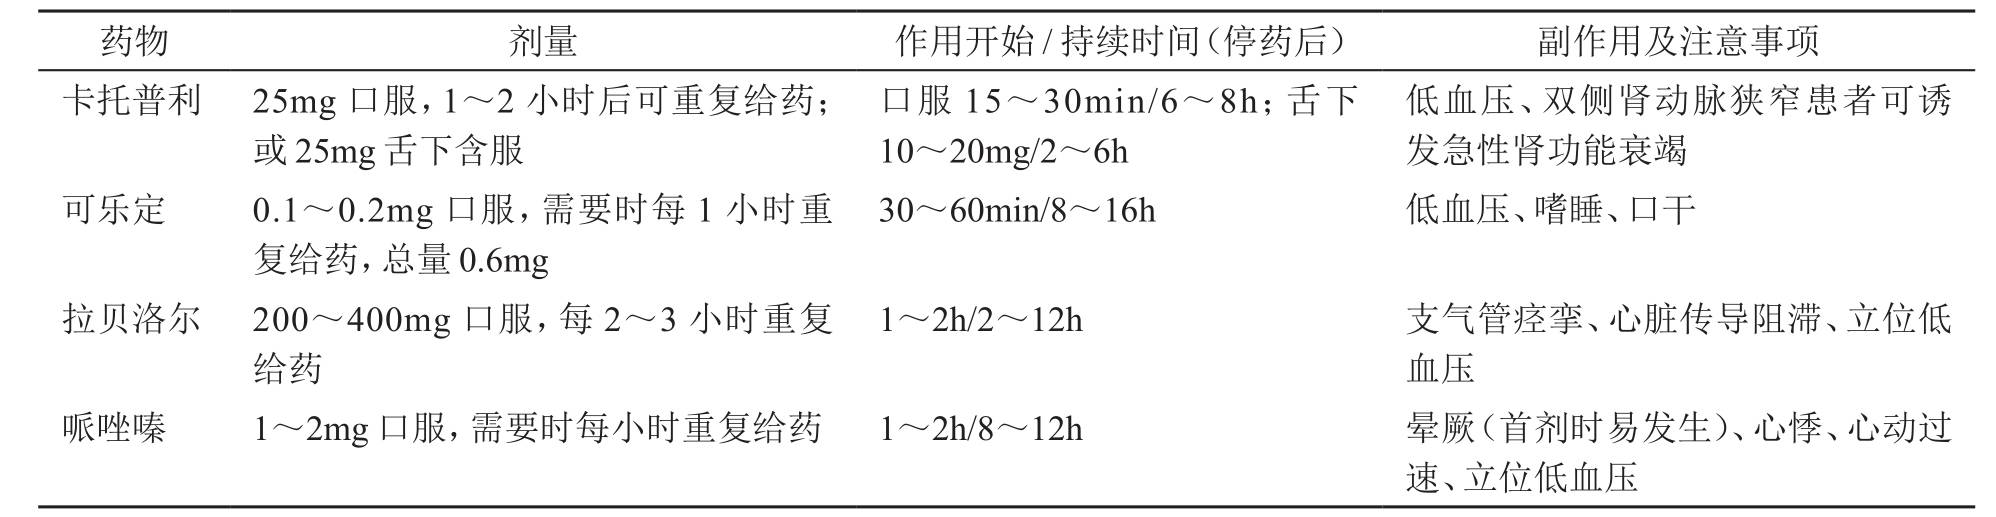
\includegraphics[width=6.64583in,height=1.70833in]{./images/Image00163.jpg}
\end{table}

\hypertarget{text00108.htmlux5cux23CHP4-7-3-2-3}{}
(三) 高血压(次)急症口服降压药物

用于高血压(次)急症的口服降压药物主要有以下几种:表\ref{tab42-4}。

\paragraph{卡托普利(captopril)}

是口服血管紧张素转换酶抑制剂的代表药物,它也可舌下含服。15分钟起效,作用持续4~6小时。初次使用时极少引起急剧低血压效应,是治疗高血压次急症的最安全口服降压药。同时给予袢利尿剂如呋塞米可增强卡托普利的效果。常用剂量为12.5~50mg/次,每日2~3次。其他常用的口服ACEI还有:依那普利、蒙诺普利、苯那普利、培哚普利。

\paragraph{可乐定(clonidine)}

是中枢α肾上腺素能激动剂,口服后30~60分钟起效,2~4小时达到最大效应。单一剂量0.2mg疗效与0.1mg/h相当。可乐定的最常见副作用是倦睡(发生率高达45\%),可能会影响对患者精神状态的评估。

\paragraph{拉贝洛尔(labetalol)}

是联合的α和β肾上腺素能受体拮抗剂,口服200~400mg,2小时起效。与其他的β受体阻滞剂一样,拉贝洛尔可引起心脏传导阻滞,加重支气管痉挛。房室传导阻滞、心动过缓、慢性充血性心衰慎用。

\paragraph{哌唑嗪(prazosin)}

是α肾上腺素能阻滞剂,可用于嗜铬细胞瘤患者的早期处理。副作用包括晕厥(首剂时易发生)、心悸、心动过速和立位低血压。

\paragraph{呋塞米(furosemide)}

是袢利尿剂,每日40~120mg,分1~3次口服,最大剂量每日160mg。迅速降低心脏前负荷,改善心衰症状,减轻肺水肿和脑水肿,特别适合于心、肾功能不全和高血压脑病的患者。作用快而强,超量应用时,降压作用不加强,不良反应反而加重。可能出现水、电解质紊乱,以及与此有关的口渴、乏力、肌肉酸痛、心律失常。少尿或无尿患者应用最大剂量后24小时仍无效时应停药。

\paragraph{硝苯地平(nifedipine)}

是短效制剂,可口服、舌下含服或咀嚼,5~10分钟起效,持续3~5小时,常用剂量为每次5~10mg,每日3次。但因其可能引起急剧且不可控制的低血压效应,及反射性心动过速,增加心肌氧耗,恶化心肌缺血而可能危及生命。这种严重的副作用是不可预测的,故目前认为应慎用于高血压危象。
\protect\hypertarget{text00109.html}{}{}

\hypertarget{text00109.htmlux5cux23CHP4-7-4}{}
参 考 文 献

1. 沈潞华.高血压急症.中国循环杂志,2009,24(3):231-233

2.
郭树彬.高血压急症的处理与靶器官保护策略.中国急救医学,2009,29(1):76-79

3. 孟庆义.急诊临床思维.北京:科学技术文献出版社,2010

4. 田国祥
,孟庆义.高血压急症治疗-尼卡地平的兴起.中国循证心血管医学杂志,2010,2(1):6-8

5. 孟庆义
.高血压急症治疗应关注肺循环.中国急救医学,2009,29(2):145-147

6. Pergolini MS. The management of hypertensive crises:a clinical
review. Clin Ter,2009,160(2):151-157

7. Rodriguez MA,Kumar SK,De Caro M. Hypertensive crisis. Curr Drug
Targets,2009,10(8):788-798

\protect\hypertarget{text00110.html}{}{}

\chapter{垂 体 危 象}

腺垂体功能减退症是指腺垂体激素分泌减少,可以是单种激素减少如生长激素(GH)缺乏或多种促激素同时缺乏。由于腺垂体分泌细胞是在下丘脑各种激素(因子)直接影响之下,腺垂体功能减退可原发于垂体病变,或继发于下丘脑病变,表现为甲状腺、肾上腺、性腺等靶腺功能减退和(或)鞍区占位性病变。临床症状变化较大,但补充所缺乏的激素治疗后症状可迅速缓解。

垂体危象是在腺垂体功能减退的基础上,血循环中肾上腺皮质激素和甲状腺激素缺乏,对外界环境变化的适应能力下降,机体抵抗力下降,在各种应激情况下,如感染、腹泻、呕吐、失水、饥饿、受寒、中暑、手术、外伤、麻醉、酗酒及使用各种镇静安眠药、降糖药等,导致患者病情发生急剧变化,可表现为高热(>
40℃),低温(< 35℃),低血糖,循环衰竭,水中毒等的一种危及生命状态。

\subsection{病因与发病机制}

垂体前叶分泌六种激素,包括生长激素(GH)、泌乳素(PRL)、卵泡刺激素(FSH)、黄体生成素(LH)、促皮质激素(ACTH)和促甲状腺素(TSH),主要管辖三个靶腺及其相应靶组织:性腺、肾上腺皮质和甲状腺。

腺垂体功能减退症是临床上常见的内分泌疾病,系因腺垂体激素分泌功能部分或全部丧失。常见病因为以下几方面:

\paragraph{垂体及附近肿瘤压迫浸润}

垂体肿瘤,鞍上及鞍旁肿瘤,各种转移性癌,淋巴瘤,白血病,组织细胞增多症等均可浸润下丘脑和垂体,引起垂体前叶功能不全。

\paragraph{产后大出血所致垂体前叶破坏及萎缩}

产妇在分娩过程中大出血,可导致垂体前叶坏死,称为希恩(Sheehan)综合征。一般认为,随着妊娠,垂体呈生理性肥大,大出血时血管痉挛,血栓形成,或产后败血症引起垂体栓塞或DIC,导致腺垂体急性坏死。神经垂体的血流供应不依赖门脉系统,故产后出血一般不伴有神经垂体坏死。

\paragraph{感染和炎症}

各种病毒、结核、梅毒、真菌感染,化脓性脑膜炎,脑膜脑炎,流行性出血热,均可引起下丘脑-垂体损伤而导致功能减退。

\paragraph{自身免疫性疾病}

常见的是自身免疫性垂体炎,好发于妊娠及产后妇女,男性少见。自身免疫性垂体炎临床多表现为垂体功能减低,鞍区肿物或垂体柄增粗,有时伴高催乳素血症,金标准是病理诊断。

\paragraph{手术 、创伤和放射损伤}

垂体瘤摘除、放疗,或鼻咽癌等颅底及颈部放疗后均可引起本症。颅底骨折、垂体柄挫伤可阻断神经与门脉系统的联系而导致腺垂体及神经垂体功能减退。

\paragraph{其他}

空泡蝶鞍,动脉硬化可引起垂体梗死,颞动脉炎,海绵窦血栓常导致垂体缺血,糖尿病性血管病变引起缺血坏死等。长期大剂量糖皮质激素治疗也可抑制相应垂体激素的分泌,突然停药可出现单一性垂体激素分泌不足的表现。

上述多种病因均可引起下丘脑和(或)垂体功能减退,若为中度或重度垂体功能减退症,未经系统和正规激素补充治疗,或终止治疗,再遇感染、外伤、手术等应激状态或处理不当,常可诱发多种代谢紊乱和器官功能失调,出现精神失常、意识模糊、神志不清、谵妄甚至昏迷诱发垂体危象。

\subsection{诊断}

\subsubsection{临床表现特点}

\hypertarget{text00110.htmlux5cux23CHP4-8-2-1-1}{}
(一) 腺垂体功能减退

腺垂体功能减退症的临床表现与患者发病的年龄、性别、受累激素种类、分泌受损程度及原发病的病理性质有关。通常GH和FSH、LH的缺乏发生最早,其次是ACTH
及TSH缺乏。当肾上腺皮质激素和(或)甲状腺激素缺乏时,机体应激能力下降。

一般情况下,垂体破坏50\%以上才出现临床症状,破坏75\%出现较明显症状,破坏95\%出现严重症状。其中以LH、FSH和PRL受累最早最严重,其次分别为TSH、ACTH。

1.ACTH缺乏引起肾上腺皮质功能不全,表现为虚弱无力,肌肉松弛,肤色浅淡,食欲下降,体重减轻,血压下降或发生直立性低血压,易发生低血糖症。

2.TSH缺乏引起继发性甲减,患者水肿,表情淡漠,畏寒,皮肤干燥,心动过缓,体温低。

3.LH、FSH缺乏引起性腺功能减退,希恩综合征表现为产后无乳,闭经,腋毛阴毛脱落,性欲减退,乳房萎缩;男性表现为阳痿,睾丸萎缩,性欲低下等。

4.原发疾病表现
,垂体及附近肿瘤可有头痛、呕吐、视力减退、视野缺损等症状。

\hypertarget{text00110.htmlux5cux23CHP4-8-2-1-2}{}
(二) 垂体危象

在全垂体功能减退症基础上
,各种应激如感染、脓毒症、腹泻、呕吐、失水、饥饿、受寒、AMI、脑卒中、手术、外伤、麻醉及使用各种镇静安眠药、降糖药等均可诱发垂体危象。垂体危象临床主要表现为以下几种类型:

\paragraph{高热型(> 40℃)}

由于体内缺乏肾上腺皮质激素,患者抵抗力降低,容易感染,感染后发生高热。

\paragraph{低温型(< 35℃)}

由于患者甲状腺激素不足,全身代谢低下,产热不足,可低于35℃,昏迷逐渐发生,皮肤苍白、干冷,脉慢而细。

\paragraph{低血糖型}

由于患者缺乏肾上腺皮质激素和甲状腺激素,肝糖原储备不足,患者不耐受饥饿;同时患者对胰岛素敏感性增加,因而容易发生低血糖甚至昏迷。

\paragraph{低血压 、循环虚脱型}

糖皮质激素不足,容易发生低钠血症;胃肠道功能紊乱、手术、感染等,失钠,致血容量减低,容易发生周围循环衰竭和休克,患者表现为食欲不振、头痛、恶心、呕吐、软弱无力,严重者精神错乱、昏迷。

\paragraph{水中毒型}

当患者饮水过多或做水负荷实验可引起血容量增加,血液稀释,原有低钠血症时更容易发生,患者表现为全身无力、头痛、恶心、呕吐、意识模糊、嗜睡、抽搐甚至昏迷。

各种类型可伴有相应的症状,突出表现为消化系统、循环系统和神经精神方面的症状,如高热、循环衰竭、休克、恶心、呕吐、头痛、神志不清、谵妄、抽搐、昏迷等。①消化系统:可在原有的厌食、腹胀、腹泻的基础上,发展为恶心、呕吐,甚至不能进食。②循环系统:低钠血症,血容量降低,表现为脉搏细弱,皮肤干冷,心率过快或过缓,血压过低,直立性低血压,虚脱,甚至休克。③精神神经系统:患者可出现精神萎靡、烦躁不安、嗜睡、神志不清、谵妄或昏迷,低血糖患者可表现为无力、出汗、视物不清、复视或昏迷。

对于既往病史不清的患者,若出现严重的循环衰竭、低血糖、淡漠、昏迷、难以纠正的低钠血症、高热以及呼吸衰竭,应当考虑垂体危象。

\subsubsection{实验室检查}

\paragraph{血常规及血生化}

严重的低钠血症最为常见,血钠通常低于120mmol/L。而合并甲状腺功能减退的患者可出现贫血,表现为红系或三系均减低。患者空腹血糖降低,二氧化碳结合力降低。伴有严重感染的患者白细胞总数和中性粒细胞数明显升高。

\paragraph{靶腺激素水平减低}

肾上腺皮质激素(血皮质醇和尿游离皮质醇)及其代谢产物(17-羟类固醇,17-酮类固醇),甲状腺激素(T\textsubscript{3}
、T\textsubscript{4} 、FT\textsubscript{3} 、FT\textsubscript{4}
)及性腺激素(雌二醇、睾酮)均降低。

\paragraph{垂体激素减少}

生长激素(GH)、促肾上腺皮质激素(ATCH)、促甲状腺激素(TSH)、促性腺激素即黄体生成素(LH)和卵泡刺激素(FSH)降低。

\paragraph{兴奋试验}

在危象治疗好转后,可行兴奋试验进一步确诊。

\subsubsection{影像学检查}

\paragraph{磁共振成像}

(MRI)薄层扫描
通常作为首选的影像学检查,可以表现为下丘脑及垂体的占位病变、弥漫性病变、囊性变或空泡蝶鞍。

\paragraph{CT增强扫描}

对于有鞍底骨质破坏的患者及垂体卒中急性期的患者,CT比MRI有价值。

\paragraph{X线平扫及断层}

可表现为蝶鞍扩大、鞍底骨质破坏等。

\subsubsection{鉴别诊断}

\paragraph{黏液性水肿昏迷}

高血脂和黏液性水肿程度明显,甲状腺激素减低,垂体TSH明显增高,垂体促激素刺激试验始终不反应;而垂体前叶功能减退危象时,各相应的促激素正常或较低,垂体促激素刺激试验呈迟发反应。

\paragraph{胰岛素瘤或糖尿病用药引起的低血糖昏迷}

此种情况昏迷者,不伴腋毛、阴毛稀少等垂体功能减退表现,垂体及靶腺激素水平正常,血胰岛素水平升高。

\paragraph{脑血管意外}

病史、临床表现及激素测定有助鉴别。

\subsection{治疗}

一旦诊断垂体危象,及早应用糖皮质激素是抢救成功的关键,剂量为开始足量,根据病情的缓解程度逐渐减量直至替代剂量,补充了糖皮质激素才能有效纠正低血糖、低血压、低钠低氯血症。但对水中毒、失钠、低温型患者,糖皮质激素剂量不可过大。若同时合并甲状腺功能减退,甲状腺激素的替代应在糖皮质激素替代之后,小剂量开始,逐渐增加甲状腺激素的用量,直至生理替代剂量,若在使用糖皮质激素之前使用较大剂量的甲状腺激素,可能因加快糖皮质激素代谢而加重危象。

\paragraph{一般治疗}

一般先静注50\%葡萄糖40~60ml,继以10\%葡萄糖500~1000ml,内加氢化可的松100~300mg滴注,但低温型昏迷患者氢化可的松用量不宜过大。

\paragraph{低温型者}

治疗与黏液性水肿昏迷者相似,可用电热毯等将患者体温回升至35℃以上,但必须注意用甲状腺激素之前(至少同时)加用适量氢化可的松,此外,严禁使用氯丙嗪、巴比妥等中枢抑制剂。

\paragraph{严重低钠血症者}

需静脉补含钠液体,补钠时应缓慢,每小时血钠提高<
0.5mmol/L,但是最关键的措施仍是补充肾上腺皮质激素。

\paragraph{水中毒性昏迷者}

应立即给予小~中量的糖皮质激素,可口服泼尼松10~25mg或氢化可的松40~80mg,每6小时1次。不能口服者将氢化可的松50~200mg(地塞米松1~5mg),加入50\%葡萄糖液40ml,缓慢静脉注射,并适当限水。

\paragraph{加强诱因控制及对症支持治疗}

患者宜进高热量、高蛋白及富含维生素膳食,还需提供适量钠、钾、氯,但不宜过度饮水,防止劳累及应激刺激。病情平稳后,如果为育龄期妇女,可加用人工月经周期治疗,男性患者可补充雄激素以维持第二性征和性功能。

激素终生替代是治疗垂体功能减退的根本,遇感染等应激时激素应加量。一旦出现表情淡漠、嗜睡、定向力障碍、昏迷、低体温、低血压、低血钠、低血糖等症状体征即可认为垂体危象可能,应及时抢救,争取时间,抽血查垂体激素及靶腺激素水平、血常规及血生化后,立即使用糖皮质激素。如为垂体肿瘤内急性出血压迫视神经、出现垂体卒中,应尽快手术治疗。
\protect\hypertarget{text00111.html}{}{}

\hypertarget{text00111.htmlux5cux23CHP4-8-4}{}
参 考 文 献

1. 顾锋.垂体危象及垂体卒中.国外医学内分泌学分册,2005,25(6):433-435

2. Kearney T,Dang C. Diabetic and endocrine emergencies. Postgrad Med
J,2007 Feb,83(976):79-86

3. Arlt W. The approach to the adult with newly diagnosed adrenal
insufficiency. J Clin Endocrinol Metab,2009,94(4):1059-1067

\protect\hypertarget{text00112.html}{}{}

\chapter{甲状腺危象}

甲状腺危象(thyroid crisis,thyroid
storm)也称甲亢危象,是一种甲状腺毒症(thyrotoxicosis)病情极度加重的状态。甲亢危象是甲状腺功能亢进症(hyperthyroidism,甲亢)最严重的并发症,起病急、病情危重,不仅可导致多脏器功能衰竭,而且可导致死亡。早期诊断、及时正确治疗是成功抢救甲亢危象的关键,但积极预防甲亢危象的发生才是最重要的。

甲亢危象不常见。随着人们对该病症认识的提高、医疗条件和技术的改善,甲亢危象已经逐步减少。国外报道甲亢危象占甲状腺毒症患者的1\%左右。北京协和医院在20世纪70年代以前的44年间收治的甲亢危象36例次,占住院甲亢患者的1.45\%,在20世纪80年代初至2009年收治甲亢危象患者24例次,占同期住院甲亢患者的0.7\%。

甲亢危象与甲状腺毒症一样,好发于女性。可发生于任何年龄段,老年人多见,小儿少(罕)见。由各种原因导致甲状腺毒症的患者发生甲亢危象的危险都是存在的,其中以弥漫性毒性甲状腺肿(Graves病)最常见,其次为多结节性毒性甲状腺肿;也见于甲状腺损伤或甲状腺炎引起的甲状腺毒症。

\subsection{病因与发病机制}

\subsubsection{甲状腺毒症的病因}

甲状腺毒症是指血循环中甲状腺激素量过多,引起以神经、循环、消化等系统兴奋性增高和代谢亢进为主要表现的一组临床综合征。根据甲状腺的功能状态,甲状腺毒症可分为甲状腺功能亢进类型和非甲状腺功能亢进类型;前者的病因主要有Graves病、多结节性毒性甲状腺肿、甲状腺自主高功能腺瘤(Plummer病)、碘致甲状腺功能亢进症(碘甲亢)、桥本甲状腺毒症、TSH分泌性垂体腺瘤等,后者包括破坏性甲状腺毒症和服用外源性甲状腺激素。由于甲状腺滤泡被炎症(如亚急性甲状腺炎、无症状性甲状腺炎、桥本甲状腺炎、产后甲状腺炎等)破坏,滤泡内储存的甲状腺激素过量进入循环引起的甲状腺毒症称为破坏性甲状腺毒症。该类型甲状腺毒症的甲状腺功能并不亢进。

\subsubsection{甲亢危象的诱因}

多种原因可引发甲亢危象,这些原因可以是单一的,也可以由几种原因合并叠加引起。

\paragraph{内科方面的诱因}

①感染:感染是引发甲亢危象最常见的内科原因。主要包括上呼吸道感染、咽炎、扁桃体炎、气管炎、支气管肺炎,其次是胃肠道和泌尿系感染,脓毒病及其他感染如皮肤感染等均少见。②应激:精神极度紧张、工作过度劳累、高温、饥饿、药物反应(如药物过敏、白细胞明显减少、洋地黄中毒等)、心绞痛、心力衰竭、糖尿病酸中毒、低血糖、高钙血症、肺栓塞、脑梗死及其他脑血管意外、妊娠(甲亢患者妊娠后未治疗的,较给予治疗者发生危象几率多达10倍以上)、分娩及妊娠高血压疾病等,均可能导致甲状腺突然释放大量甲状腺激素,引起甲亢危象。③不适当停用碘剂药物:应用碘剂治疗甲亢中,突然停用碘剂,原有甲亢表现可迅速加重,因为碘化物可以抑制甲状腺激素结合蛋白质的水解,使甲状腺激素释放减少。此外,细胞内碘化物增加超过临界浓度时,可使甲状腺激素的合成受抑制,由于突然停用碘剂,甲状腺的滤泡上皮细胞内碘的浓度减低,抑制效应消失,甲状腺内原来贮存的碘又能合成甲状腺激素,释入血中,使病情迅速增重。不规则使用或停用硫脲类抗甲状腺药,偶尔也会引发甲亢危象,但这种情况并不多见。④少见原因:由于放射性碘治疗甲亢引起的放射性甲状腺炎、甲状腺活体组织检查,以及过多或过重或反复触摸甲状腺,使甲状腺损伤,均可使大量的甲状腺激素在短时间内释放进入血中,引起病情突然增重。也有称给碘剂(碘造影剂或口服碘)也可引发甲亢危象。此甲亢并发症也会发生于以前存在甲状腺毒症治疗不充分或始终未进行治疗的患者。

\paragraph{外科方面的诱因}

甲亢患者在手术后4~16小时内发生危象者,要考虑危象与手术有关;而危象在16小时以后出现者,尚需寻找感染病灶或其他原因。由手术引起甲亢危象的原因有:①甲亢病情未被控制而行手术:甲亢患者术前未用抗甲状腺药做准备;或因用药时间短或剂量不足,准备不充分;或虽用抗甲状腺药,但已经停药过久,手术时甲状腺功能仍处于亢进状态;或是用碘剂做术前准备时,用药时间较长,作用逸脱,甲状腺又能合成及释放甲状腺激素。②术中释放甲状腺激素:手术本身的应激、手术时挤压甲状腺,使大量甲状腺激素释放进入血中。另外,采用乙醚麻醉时也可使组织内的甲状腺激素进入末梢血中。③剖宫产或甲状腺以外的其他手术。

一般来说,内科方面的原因诱发的甲亢危象,其病情较外科方面的原因引起的甲亢危象更为常见,程度也严重。

\subsubsection{发病机制}

甲亢危象发生的确切机制尚不完全清楚,可能与下列因素有关,这些因素可以解释部分患者甲亢危象的发生原因,尚不能概括全部甲亢危象发生机制。

\paragraph{大量甲状腺激素释放至血循环}

它不是导致甲亢危象发生最主要的原因,但与服用大量甲状腺激素、甲状腺手术、不适当的停用碘剂以及放射性碘治疗后甲亢危象发生有关。

\paragraph{血中游离甲状腺激素增加}

感染、甲状腺以外其他部位的手术等应激,可使血中甲状腺激素结合蛋白质浓度减少,与其结合的甲状腺激素解离,血中游离甲状腺激素增多。这可以解释部分甲亢危象患者的发病。

\paragraph{周围组织对甲状腺激素反应的改变}

由于某些因素的影响,使甲亢患者身体各系统的脏器及周围组织对过多的甲状腺激素适应能力减低,由于此种失代偿而引起危象。临床上见到在甲亢危象时,有多系统的功能衰竭、血中甲状腺激素水平可不升高,以及在一些患者死后尸检所见无特殊病理改变,均支持对甲状腺激素反应的改变的这种看法。

\paragraph{儿茶酚胺结合和反应力增加}

在甲亢危象发病机制中儿茶酚胺起关键作用。甲亢危象患者的儿茶酚胺结合位点增加,对肾上腺素能刺激反应力增加,阻断交感神经或服用抗交感神经或β-肾上腺素能阻断剂后甲亢和甲亢危象的症状和体征可明显改善。

\paragraph{甲状腺素在肝中清除降低}

手术前、后和其他的非甲状腺疾病的存在、进食量减少,热量不足,均引起T\textsubscript{4}
清除减少,血中甲状腺素含量增加。

\subsection{诊断}

\subsubsection{临床表现特点}

多数患者原有明显甲状腺毒症相关临床表现,在诱发因素作用下出现临床表现明显加重为甲亢危象,少数患者起病迅猛,快速进入到甲亢危象。

甲亢危象典型临床表现包括:

\paragraph{高热}

本症发生体温急骤升高,多常在39℃以上,伴大汗淋漓,皮肤潮红,严重者,继而汗闭,皮肤苍白和脱水。高热是甲亢危象的特征性表现,是与重症甲亢的重要鉴别点。

\paragraph{中枢神经系统异常}

精神变态、焦虑,肢体震颤、极度烦躁不安、甚至出现谵妄、嗜睡,最后陷入昏迷状态。部分患者可伴有脑血管病发生,脑出血或脑梗死。

\paragraph{心血管功能异常}

心动过速,大于140次/分以上,甚至超过160次/分。伴有各种形式的快速心律失常,特别是快速房颤。有些患者可出现心绞痛,心力衰竭,收缩压增高、脉压显著增加。随病情恶化,最终血压下降,陷入休克。一般来说,甲亢伴有甲亢性心脏病的患者,容易发生甲亢危象,当发生危象以后,会促使心脏功能进一步恶化。

\paragraph{消化功能异常}

食欲极差,进食减少,恶心,呕吐频繁,腹痛,腹泻明显。腹痛及恶心、呕吐可发生在病的早期。病后体重锐减。肝脏可肿大,肝功能不正常,随病情的进展,肝细胞功能衰竭,常出现黄疸。黄疸的出现则预示病情严重及预后不良。

\paragraph{电解质紊乱}

由于进食差,呕吐、腹泻以及大量出汗,最终出现电解质紊乱,约半数患者有低血钾症,1/5的患者血钠减低。一些患者出现酸碱失衡。

有些患者甲亢危象临床征象不明显,称做“安静”类型。临床表现为行为改变,睡眠及记忆力障碍,痴呆,抑郁,嗜睡以及被动处事等。

很少一部分患者临床症状和体征甚至更不典型,表现为“淡漠型”。其特点是表情淡漠、木僵、嗜睡、反射降低、低热、明显乏力、心率慢、脉压小及恶病质,甲状腺常仅轻度肿大,最后陷入昏迷,甚而死亡。多见于老年及体质极度衰弱者。

\subsubsection{实验室检查}

危象时,血白细胞数可升高,伴轻度核左移。可有不同程度的肝功能异常、血清电解质异常,包括轻度的血清钙和轻度血糖水平升高。

危象时,血清甲状腺激素水平升高,但升高的程度不一致,多数升高程度与一般甲状腺毒症患者比较没有更显著增高,危象病程后期有些患者血清T\textsubscript{3}
水平甚至在正常范围。因此,通过血中甲状腺激素水平高低对甲亢危象的诊断帮助不大。

\subsubsection{诊断标准和注意事项}

任何一个甲状腺毒症的患者,特别是未经正规治疗、或治疗中断及有上述的内科及外科方面的诱因存在时,出现原有的甲亢病情突然明显增重,应考虑有甲亢危象的可能。

甲亢病史和一些特殊体征,如突眼,甲状腺肿大或其上伴血管杂音,以及胫骨前黏液性水肿、皮肤有白癜风及杵状指等表现提示存在甲亢可能,对诊断甲亢危象均有帮助。临床上怀疑有甲亢危象时,可先取血备查甲状腺激素。

甲亢危象尚无统一诊断标准。Wartofsky和Peele介绍用打分法(即根据体温高低,中枢神经系统影响,胃肠功能的损害,心率的增加,充血性心衰表现程度,心房纤颤的有无,诱因的存在与否来评分,依据打分后的最后积分<
25,25~44及>
45来判断为不能诊断、怀疑或确诊)。北京协和医院通过多年的临床实践,将甲亢危象大体分为两个阶段,即体温低于39℃和脉率在159次/分以下,多汗、烦躁、嗜睡、食欲减退、恶心以及大便次数增多等定为甲亢危象前期;而当患者体温超过39℃,脉率多于160次/分,大汗淋漓或躁动,谵妄,昏睡和昏迷,呕吐及腹泻显著增多等,定为甲亢危象。在病情处于危象前期时,如未被认识、未得到及时处理,会发展为危象。甲亢患者当因各种原因使甲亢的病情加重时,只要具备上述半数以上危象前期诊断条件,即应按危象处理。

\subsection{治疗}

不论甲亢危象前期或甲亢危象一经诊断,就应立即开始治疗,一定不要等待血清甲状腺激素的化验结果,才开始治疗。治疗的目的是纠正严重的甲状腺毒症和诱发疾病,保护脏器功能,维持生命指征。对怀疑有甲亢危象的患者,开始治疗时,应当在加强医疗病房(ICU)进行持续监护。

\subsubsection{保护机体脏器、防止功能衰竭}

改善危重病况,积极维护生命指征是救治的首要目标。

\paragraph{降温}

发热轻者,用退热剂,可选用对乙酰氨基酚(扑热息痛),冰袋,室内用电风扇(及)适当的空调也需要。不宜用阿司匹林。大剂量的阿司匹林可增高患者的代谢率,还可与血中的T\textsubscript{3}
及T\textsubscript{4}
竞争结合TBG及TBPA,使血中游离甲状腺激素增多。有高热者,须积极物理降温,如电风扇、冰袋、空调,必要时可用人工冬眠{[}哌替啶(度冷丁)100mg,氯丙嗪及异丙嗪各50mg,混后静脉持续泵入{]}。

\paragraph{给氧和支持治疗}

持续给氧是必要的。因高热,呕吐及大量出汗,极易发生脱水及高钠血症,需补充水及注意纠正电解质紊乱。补充葡萄糖可提供必需的热量和糖原。还应补充大量维生素。有心力衰竭或有肺充血存在,应积极处理,应用洋地黄及利尿剂。对有心房纤颤、房室传导阻滞、心率增快的患者,应当使用洋地黄及其衍生物或钙离子通道阻断剂。

\subsubsection{减少甲状腺激素的合成和释放}

\paragraph{抑制甲状腺激素的合成}

抑制甲状腺激素的合成可选用硫脲类抗甲状腺药。口服或经胃管鼻饲或必要时直肠给药,大剂量硫脲类药物(丙硫氧嘧啶,PTU
600~1000mg/d,分次用),在1小时内可阻止甲状腺内碘化物有机结合。此后每日给用维持剂量(相当于PTU
300~600mg/d,分次给药)。甲亢危象时选用PTU优于甲巯咪唑,PTU不仅可抑制甲状腺激素的合成,还可以抑制甲状腺外T\textsubscript{4}
向T\textsubscript{3} 转化。用PTU 1天以后,血中的T\textsubscript{3}
水平可降低50\%。

\paragraph{抑制甲状腺激素的释放}

用硫脲类抗甲状腺药1小时后,开始给碘剂,迅速抑制TBG水解,从而减少甲状腺激素的释放。一般每日口服复方碘溶液(Lugol液)30滴(也有用5滴每6小时一次),或静脉滴注碘化钠1~2g(或0.25g/6h),或复方碘溶液3~4ml/1000~2000ml
5\%葡萄糖溶液中。若碘化物的浓度过高或滴注过快易引起静脉炎。既往未用过碘剂者,使用碘剂效果较好。有报告在碘化物中用5'脱碘酶的强抑制剂胺碘苯丙酸钠(sodium
ipodate)0.5g,每日2次,或0.25g/6h,可减缓甲状腺激素从甲状腺的释放,或用碘番酸钠(sodium
iopanoate)替代碘化物更有效。

\subsubsection{降低循环中甲状腺激素水平}

硫脲类抗甲状腺药和碘化物只能减少甲状腺激素的合成和释放,不能快速降低已经释放到血中的甲状腺激素水平,尤其是T\textsubscript{4}
,它的半衰期为6.1天,且绝大部分是与血浆蛋白质结合的,在循环中保留的时间相当长。文献中介绍可迅速清除血中过多的甲状腺激素的方法有:换血法、血浆除去法和腹膜透析法,这些方法均较复杂,应用经验较少。

\subsubsection{降低周围组织对甲状腺激素的反应}

对已经释入血中的甲状腺激素,应设法减低末梢组织对其反应。抗交感神经药物可减轻周围组织对儿茶酚胺作用。常用的有:

\paragraph{β-肾上腺素能阻断剂}

对抗肾上腺素能的药物对循环中甲状腺激素能间接发挥作用。在无心功能不全时,β-肾上腺素能阻断剂用来改善临床表现。严重甲状腺毒症患者能发展为高排出量的充血性心力衰竭,β-肾上腺素能阻断剂的对抗可进一步减少心脏的排出。常用的是普萘洛尔(心得安),甲亢患者用本品后,虽然对甲状腺功能无改善,但用药后患者的兴奋、多汗、发热、心率增快等均有好转。目前认为本品有抑制甲状腺激素对交感神经的作用,也可较快的使血中T\textsubscript{4}
转变为T\textsubscript{3}
降低。用药剂量需根据具体情况决定,危象时一般每6小时口服40~80mg,或静脉缓慢注入2mg,能持续作用几小时,可重复使用。心率常在用药后数小时内下降,继而体温、精神症状,甚至心律失常(期前收缩、心房纤颤)也均可有明显改善。严重的甲状腺毒症患者可发展为高排出量的充血性心力衰竭,β-肾上腺素能阻断剂可进一步减少心排血量。但对有心脏储备功能不全、心脏传导阻滞、心房扑动、支气管哮喘等患者,应慎用或禁用。使用洋地黄制剂心力衰竭已被纠正,在密切观察下可以使用普萘洛尔或改用超短效的艾司洛尔(esmolol),静脉使用。

\paragraph{利血平}

消耗组织内的儿茶酚胺,大量时有阻断作用,减轻甲亢在周围组织的表现。首次可肌注2.5~5mg,以后每4~6小时注射2.5mg,约4小时以后危象表现减轻。利血平可抑制中枢神经系统及有降血压作用,用时应予考虑。

\subsubsection{糖皮质激素的使用}

甲亢危象时肾上腺皮质激素的需要量增加,此外,甲亢时糖皮质激素代谢加速,肾上腺存在潜在的储备功能不足,在应激情况下,激发代偿分泌更多的皮质激素,导致皮质功能衰竭。另外肾上腺皮质激素还可抑制血中T\textsubscript{4}
转换为T\textsubscript{3}
。因此,抢救甲亢危象时需使用糖皮质激素。皮质激素的用量是相当于氢化可的松200~300mg/d,或地塞米松4~8mg/d,分次使用。

\subsection{预后}

甲亢危象死亡率为20\%以上(20\%~50\%)。治疗后成功者多在治疗后1~2天内好转,1周内恢复。北京协和医院的36例次危象患者,平均在抢救治疗后3天内脱离危险,7(1~14)天恢复。开始治疗后的最初3天是抢救的关键时刻。危象消失以后,碘剂及皮质激素可逐渐减药、停用,做甲亢病的长期治疗安排。
\protect\hypertarget{text00113.html}{}{}

\hypertarget{text00113.htmlux5cux23CHP4-9-5}{}
参 考 文 献

1. 白耀.甲状腺病学:基础与临床.北京:科学技术文献出版社,2003:266-271

2. LW. Braverman,RD. Utiger. Werner & Ingbar's The Thyroid a
fundamental and clinical text. Ninth edition. Philadelphia:Lippincott
William & Wilkins,2005:651-657

\protect\hypertarget{text00114.html}{}{}

\chapter{甲状腺功能减退危象}

甲状腺功能减退症(hypothyroidism,甲减)是由各种原因导致的低甲状腺激素血症或甲状腺激素抵抗而引起的全身性低代谢综合征,其病理特征是黏多糖在组织和皮肤堆积,表现为黏液性水肿(myxedema)。甲状腺功能减退危象(hypothyroidism
crisis,HC),又称为黏液性水肿昏迷,是甲状腺功能低下失代偿的一种严重的临床状态,病情重笃,往往威胁患者生命,临床表现复杂,病史隐匿,易误诊误治。

本病的初始阶段往往伴有不同的诱发疾病与诱发因素,若不能及时诊断与治疗,进一步发展可使心血管系统与神经系统发生致命性的功能衰竭。在老年人,这种失代偿状况尤为突出,故本症多发生于老年患者。

\subsection{病因与发病机制}

\subsubsection{病因与分类}

\hypertarget{text00114.htmlux5cux23CHP4-10-1-1-1}{}
(一) 甲减的分类方法

\paragraph{根据病变发生的部位分类}

①原发性甲减(primary
hypothyroidism):由于甲状腺腺体本身病变引起的甲减,占全部甲减的95\%以上,且90\%以上原发性甲减是由自身免疫、甲状腺手术和甲亢\textsuperscript{131}
I治疗所致。②中枢性甲减(central
hypothyroidism):由下丘脑和垂体疾病引起的促甲状腺激素释放激素(TRH)或者促甲状腺激素(TSH)产生和分泌减少所致的甲减。垂体外照射、垂体大腺瘤、颅咽管瘤及产后大出血是其较常见的原因;其中由于下丘脑病变引起的甲减称为三发性甲减(tertiary
hypothyroidism)。③甲状腺激素抵抗综合征:由于甲状腺激素在外周组织实现生物效应障碍引起的综合征。

\paragraph{根据病变的原因分类}

有药物性甲减、\textsuperscript{131}
I治疗后甲减、手术后甲减、特发性甲减、垂体或下丘脑肿瘤手术后甲减等。

\paragraph{根据甲状腺功能减退的程度分类}

①临床甲减(overt
hypothyroidism):具有甲状腺功能减退的临床表现及血清甲状腺激素(T\textsubscript{3}
、T\textsubscript{4} 、FT\textsubscript{4}
)降低。②亚临床甲减(subclinical
hypothyroidism):指临床上无或仅有少许甲减症状,血清FT\textsubscript{3}
、及FT\textsubscript{4}
正常而TSH水平升高。需根据TSH测定和(或)TRH试验确诊。

\paragraph{以甲减起病时年龄分类}

①功能减退始于胎儿期或出生不久的新生儿者,称为呆小病(又称克汀病);②功能减退始于发育前儿童期者,称为幼年甲减;③功能减退始于成人期者,称为甲减。

\hypertarget{text00114.htmlux5cux23CHP4-10-1-1-2}{}
(二) 病因

成人甲减的主要病因是
:①自身免疫损伤:最常见的原因是自身免疫性甲状腺炎,包括桥本甲状腺炎、萎缩性甲状腺炎、产后甲状腺炎等;②甲状腺破坏:包括手术、\textsuperscript{131}
I治疗。甲状腺次全切除、\textsuperscript{131}
I治疗Graves病,十年的甲减累积发生率分别为40\%、40\%~70\%。③碘过量:可引起具有潜在性甲状腺疾病者发生一过性甲减,也可诱发和加重自身免疫性甲状腺炎。含碘药物胺碘酮诱发甲减的发生率是5\%~22\%。④抗甲状腺药物:如锂盐、硫脲类、咪唑类等。HC多见于年老长期未获治疗者,受寒及感染是最常见的诱因。

\subsubsection{发病机制}

\paragraph{氧耗与体热}

患者的机体氧耗和体热的产生均相应地下降,同时通过神经血管调节,限制皮肤的血液循环,以减少体热的丢失。在老年患者,氧耗与体热产生的下降更为明显,且代偿能力差,故易出现低体温,在冬季甚至在正常的温度下均可发生。

\paragraph{心血管系统}

心肌黏液性水肿导致心肌收缩力损伤、心动过缓、心排出量下降。ECG示低电压。由于心肌间质水肿、非特异性心肌纤维肿胀、左心室扩张和心包积液导致心脏增大,有学者称之为甲减性心脏病。冠心病在本病中高发。10\%的患者伴发高血压。HC晚期,血压转为持续性下降。

\paragraph{交感神经系统}

循环的儿茶酚胺(去甲肾上腺素和肾上腺素)水平一般正常,但终末器官对儿茶酚胺的反应性明显低下。β-肾上腺素能反应性的低下主要由于β-受体数量的减少,G蛋白调节异常和磷酸二酯酶活性增加。相反在β-肾上腺素能反应受损的同时,α-肾上腺素能活性却完整地保持正常。当输注小剂量肾上腺素时,正常人表现为心动过速与血管扩张;但在HC患者却表现为血管收缩和高血压反应。β-肾上腺素能活性低下,也损害了热能产生的反应能力,一旦热量丢失过多,就不能保持正常体温。

\paragraph{呼吸系统}

甲状腺功能低下,可以损害对高碳酸血症的呼吸反应能力,导致低通气量,极易发生CO\textsubscript{2}
潴留,当并发肺部感染时,CO\textsubscript{2} 潴留尤为加重。

\paragraph{肾脏功能}

水分排出受损,易发生低钠血症。水潴留主要由于血抗利尿激素(ADH)水平升高和肾脏血流量减少所致。后者与功能性血容量减少、心排血量下降有关。低钠血症,特别是在老年患者,常可进一步促使中枢神经系统损害,加重HC的神经精神异常。

\paragraph{代谢系统}

易发生低血糖。主要由于胰岛素清除率下降和糖原生成减少。另外,对肾上腺素与胰高血糖素的反应能力也受到了损害。血皮质醇虽然仍可维持在正常的基础水平,但其应激反应却严重受损。在一般情况下,几乎各种药物的清除率都是下降的,从而易致药物中毒,许多常用药物,如地高辛、利尿药与镇静药等,若给予常规剂量均可致药物中毒。此外,血浆肌酶包括转氨酶、磷酸肌酸激酶和乳酸脱氢酶及其异构形式,均易呈现升高。这些肌酶升高,估计是由于从骨骼肌向外渗漏及清除率下降而造成的。

\paragraph{血液系统}

由于下述四种原因发生贫血:①甲状腺激素缺乏引起Hb合成障碍;②肠道吸收铁障碍引起铁缺乏;③肠道吸收叶酸障碍引起叶酸缺乏;④恶性贫血是与自身免疫性甲状腺炎伴发的器官特异性自身免疫病。

\subsection{诊断}

\paragraph{病史}

HC多见于年老长期未获治疗者。昏迷前常有乏力、怠惰、反应迟缓、怕冷、食欲不振、便秘、体重增加、声音粗哑和听力下降,少数患者昏迷前有情绪抑郁或胡言乱语,类似精神分裂症的表现。如果患者有甲状腺疾病、甲状腺手术、放射碘治疗或其颈部放射线照射或分娩大出血与休克的病史,或其他垂体与下丘脑疾病史则有助于诊断。

\paragraph{临床表现特点}

HC见于病情严重的甲减患者,多在冬季寒冷时发病。诱因为严重的全身性疾病、甲状腺激素替代治疗中断、寒冷、手术、麻醉和使用镇静药等。临床表现为嗜睡、低体温(<
35℃)、呼吸徐缓、心动过缓、血压下降、四肢肌肉松弛、反射减弱或消失,甚至昏迷、休克、肾功能不全危及生命。

本病常有典型的甲减面容,如水肿、呆滞、唇厚、鼻宽、舌大、面色蜡黄、粗糙。全身皮肤发凉、水肿、弹性差,头发稀、干、缺少光泽,眉毛少。多数患者甲状腺不大。约1/3患者有心界扩大或心包积液,心音低钝而缓慢。胸腔积液或腹水也不少见。常有肝大。四肢肌张力低,腱反射低或消失。

\paragraph{实验室检查}

血清TSH升高、TT\textsubscript{4} 、FT\textsubscript{4}
降低为原发性甲减,在严重病例血清TT\textsubscript{3}
和FT\textsubscript{3}
减低;亚临床甲减仅有血清TSH升高,血清T\textsubscript{4}
或T\textsubscript{3} 正常。若TSH降低或正常,TT\textsubscript{4}
、FT\textsubscript{4}
降低,考虑中枢性甲减;做TRH刺激试验有助鉴别:静注TRH后,血清TSH不增高者提示为垂体性甲减,延迟增高者为下丘脑性甲减,在增高的基值上进一步增高者提示原发性甲减。

\paragraph{鉴别诊断}

血清TSH升高、TT\textsubscript{4} 、FT\textsubscript{4}
降低是诊断甲减的必备条件。鉴别诊断包括:①贫血:应与其他原因的贫血鉴别。②蝶鞍增大:应与垂体瘤鉴别。原发性甲减时TRH分泌增加可致高PRL血症、溢乳及蝶鞍增大,酷似垂体催乳素瘤,可行MRI检查鉴别。③心包积液:应与其他原因的心包积液鉴别。④水肿:主要与特发性水肿鉴别。⑤低T\textsubscript{3}
综合征:也称为甲状腺功能正常的病态综合征(euthyroid sick
syndrome,ESS),指非甲状腺疾病原因引起的伴有低T\textsubscript{3}
的综合征。严重的全身性疾病、创伤和心理疾病等都可导致甲状腺激素水平的改变,它反映了机体内分泌系统对疾病的适应性反应。主要表现在血清TT\textsubscript{3}
、FT\textsubscript{3} 水平降低,血清rT\textsubscript{3}
增高,血清T\textsubscript{4}
、TSH水平正常。疾病的严重程度一般与T\textsubscript{3}
降低的程度相关,疾病危重时也可出现T\textsubscript{4} 水平降低。

\subsection{治疗}

\paragraph{补充甲状腺激素}

HC患者都应给予甲状腺激素治疗,以逆转甲状腺功能低下状态,适应感染或其他原因的应激状况。首选L-T\textsubscript{3}
静脉注射,每4小时10μg,直至患者症状改善,清醒后改为口服;或L-T\textsubscript{4}
首次静脉注射300μg,以后每日50μg,至患者清醒后改为口服。如无注射剂可予片剂研细加水鼻饲,L-T\textsubscript{3}
20~30μg,每4~6小时1次,以后每6小时5~15μg;或L-T\textsubscript{4}
首次100~200μg,以后每日50μg,至患者清醒后改为口服。

\paragraph{对症支持治疗}

①保暖;②保持呼吸道通畅,供氧,必要时行气管插管或切开,机械通气;③静滴氢化可的松200~300mg/d,患者清醒后逐渐减量;④纠正水电解质紊乱,但入水量不宜过多,以避免水中毒、低钠血症及心力衰竭的发生或加重;⑤控制感染:细菌感染是HC最普通的诱发因素。在情况未明之前,所有的HC患者都应该疑及感染存在的可能。并在培养结果出来之前,静脉给予广谱抗生素治疗;⑥积极治疗原发疾病。

患者治疗中应注意:①L-T\textsubscript{4}
剂量不要随意增大,尤其中老年患者可能有并存的冠心病,如L-T\textsubscript{4}
剂量过大,有引致急性心肌梗死的危险;②遇有严重肺部感染的HC患者,应及时气管切开,并使用机械通气,以及早改善通气状况;③当HC患者血压下降时,切勿随意使用血管性升压药,而应静脉补充液体,以扩张血容量;④遇低体温的患者,切勿随意从外部加温。

HC患者经上述治疗,24小时左右病情有好转,则一周后可逐渐恢复;如24小时后不能逆转,多数不能挽救。

甲减患者,一般不能治愈,需要终生用甲状腺激素替代治疗。治疗的目标是将血清TSH和甲状腺激素水平恢复到正常范围内。治疗的剂量取决于患者的病情、年龄、体重和个体差异。首选左甲状腺素(L-T\textsubscript{4}
),其半衰期为7天,吸收缓慢,每天晨间服药一次即可维持较稳定的血药浓度。长期替代治疗维持量成年患者约50~200μg/d(1.6~1.8μg/kg)。儿童需要较高的剂量,大约2.0μg/(kg•d);老年患者则需要较低的剂量,大约1.0μg/(kg•d);妊娠时的替代剂量需要增加30\%~50\%;甲状腺癌术后的患者需要剂量大约2.20μg/(kg•d)。一般初始剂量为25~50μg/d,每1~2周增加12.5~25μg/d,直至达到治疗目标。在老年和缺血性心脏病患者,初始剂量为12.5~25μg/d,每2~4周增加12.5~25μg/d,以避免诱发或加重冠心病。补充甲状腺激素,重新建立下丘脑-垂体-甲状腺轴的平衡一般需要4~6周,所以治疗初期,每4~6周测定激素指标。然后依据检查结果调整L-T\textsubscript{4}
剂量,直到达到治疗目标。治疗达标后,需要每6~12个月复查一次激素指标。L-T\textsubscript{3}
(60~100μg/d)起效快、作用强,但持续时间短,一般不用于替代治疗。甲状腺片是动物甲状腺的干制剂,因其甲状腺激素含量不稳定和T\textsubscript{3}
含量过高已很少使用。

对亚临床甲减,在下述情况需要给予L-T\textsubscript{4}
治疗:高胆固醇血症、血清TSH > 10mU/L。
\protect\hypertarget{text00115.html}{}{}

\hypertarget{text00115.htmlux5cux23CHP4-10-4}{}
参 考 文 献

1. 陆再英,钟南山.内科学.第7版.北京:人民卫生出版社,2008

2. 陈灏珠 ,林果为.实用内科学.第13版.北京:人民卫生出版社,2009

3. 张文武 .急诊内科学.第2版.北京:人民卫生出版社,2007

\protect\hypertarget{text00116.html}{}{}

\chapter{肾上腺危象}

肾上腺危象(adrenal crisis)亦称急性肾上腺皮质功能减退症(acute
adrenocortical hypofunction)或艾迪生病危象(Addisonian
crisis),是指肾上腺皮质功能急性衰竭所致的危重综合征。病因多由于肾上腺皮质严重破坏致肾上腺皮质激素绝对不足,或慢性肾上腺皮质功能减低,患者在某种应激情况下肾上腺皮质激素相对不足所致。主要临床表现为高热、胃肠功能紊乱、循环虚脱、神志淡漠、萎靡或躁动不安、谵妄甚至昏迷,诊治稍失时机将威胁患者生命。

\subsection{病因与发病机制}

肾上腺危象的常见病因有:

1.急性肾上腺皮质出血 、坏死
①最常见的病因是感染。严重感染脓毒症合并全身和双侧肾上腺出血,如流行性脑脊髓膜炎合并的Waterhause-Friderichsen综合征、流行性出血热合并肾上腺出血等;②全身性出血性疾病合并肾上腺出血,如血小板减少性紫癜、DIC、白血病等;③癌瘤的肾上腺转移破坏;④外伤引起肾上腺出血或双侧肾上腺静脉血栓形成,以及抗凝药物治疗引起的肾上腺出血等。

2.肾上腺双侧全部切除
,或一侧全切、另侧90\%以上次全切除后,或单侧肿瘤切除而对侧已萎缩者,如术前准备不周、术后治疗不当或激素补给不足、停药过早等均可发生本症。

3.原发和继发性慢性肾上腺皮质功能不全患者
,在下列情况下可发生肾上腺危象:①Addison患者和肾上腺次全切除术后患者,在感染、劳累、外伤、手术、分娩、呕吐、腹泻和饥饿等应激情况下可致肾上腺危象;②长期激素替代治疗患者突然减停激素;③垂体功能减低患者如Sheehan征在未补充激素情况下给予甲状腺素或胰岛素时也可能诱发肾上腺危象。

4.长期大剂量肾上腺皮质激素治疗过程中
,由于患者垂体、肾上腺皮质已受重度抑制而呈萎缩,如骤然停药或减量过速,可引起本症。

肾上腺皮质激素是维持人的生命活动所必需的。正常人在严重应激情况下皮质醇分泌增加10倍于基础水平,但慢性肾上腺皮质功能减低、肾上腺皮质破坏的患者则不仅没有相应的增加,反而是肾上腺皮质激素严重不足。当盐类皮质激素不足时,肾小管回吸收Na\textsuperscript{+}
不足,失水、失Na\textsuperscript{+} ,K\textsuperscript{+}
、H\textsuperscript{+}
潴留;而糖皮质激素不足除糖原异生减弱致低血糖外,也有与盐皮质激素对水盐相同的作用,由于失Na\textsuperscript{+}
、失水引起血容量减少,血压下降以致虚脱和休克,引起肾上腺危象。

\subsection{诊断}

\subsubsection{临床表现特点}

肾上腺危象的发病可呈急性型,即可因皮质激素缺乏或严重应激而骤然发病;也可以呈亚急性型,主要是由于部分皮质激素分泌不足或轻型应激所造成,临床上发病相对缓慢,但疾病晚期也可以表现为严重的急性型。发生危象时,即具有共同的临床表现,也可因原发病不同而表现出各自的特点。

\paragraph{原发病的不同与起病特点}

各种病因所致的肾上腺危象本身的表现是相同的,它们之间的鉴别有赖于发生危象前各自的临床特征;危象的诱因和起病特点也有参考价值。①手术所致的肾上腺危象多于术后即发生,因失盐、失水有一个过程,常于48小时后症状明显。②难产分娩的新生儿若有肾上腺出血也常在出生后数小时至1~2天内发生危象。③弥散性血管内凝血所致者,常有严重的感染、休克、出血倾向、缺氧发绀及多器官栓塞等表现,凝血机制检查有异常发现。④流脑所致者,有烦躁、头痛呕吐、神志改变、颅内压增高、高热、皮肤黏膜紫斑、白细胞升高、脑脊液异常等。⑤慢性肾上腺皮质功能减退症常有明显色素沉着、消瘦、低血压、反复昏厥发作等病史。⑥长期应用肾上腺皮质激素者有向心性肥胖、多血质、高血压、肌肉消瘦、皮肤薄等库欣综合征表现。⑦肾上腺动静脉中血栓形成时,可出现骤然腹痛,疼痛位于患侧脐旁约在肋缘下6.5cm,一般早期无高热、休克与心率及呼吸呈显著加速等表现。

\paragraph{肾上腺危象的共同表现}

典型的肾上腺危象的表现有:

\hypertarget{text00116.htmlux5cux23CHP4-11-2-1-2-1}{}
(1) 循环系统:

心率快,可达160次/分钟以上,心律失常,脉搏细弱,全身皮肤湿冷、四肢末梢发绀,血压下降,虚脱,休克。

\hypertarget{text00116.htmlux5cux23CHP4-11-2-1-2-2}{}
(2) 消化系统:

食欲不振甚至厌食,恶心、呕吐,腹痛、腹泻、腹胀。部分病例的消化道症状特别明显,出现严重腹痛、腹肌紧张、反跳痛,酷似外科急腹症。

\hypertarget{text00116.htmlux5cux23CHP4-11-2-1-2-3}{}
(3) 神经系统:

极度孱弱,萎靡不振,烦躁不安、谵妄,逐渐出现淡漠、嗜睡、神志模糊,严重者乃至昏迷。有低血糖者常有出汗、震颤、视力模糊、复视,严重者精神失常、抽搐。

\hypertarget{text00116.htmlux5cux23CHP4-11-2-1-2-4}{}
(4) 泌尿系统:

因循环衰竭、血压下降,导致肾功能减退,血中尿素氮增高,出现少尿、无尿等。

\hypertarget{text00116.htmlux5cux23CHP4-11-2-1-2-5}{}
(5) 全身症状:

极度乏力,严重脱水(细胞外液容量丧失约1/5)。绝大多数有高热,亦可有体温低于正常者。最具特征性者为全身皮肤色素沉着加深,尤以暴露处、摩擦处、掌纹、乳晕、瘢痕等处为明显,黏膜色素沉着见于齿龈、舌部、颊黏膜等处,系垂体ACTH、黑素细胞刺激素(MSH)分泌增多所致。

\paragraph{肾上腺切除后发生本症的两种类型}

①糖皮质激素缺乏型:一般出现于停止补充可的松治疗1~2天后,有厌食、腹胀、恶心、呕吐、精神萎靡、疲乏嗜睡、肌肉僵硬、血压下降等表现。严重者可有虚脱、休克、高热等危象。②盐皮质激素缺乏型:由于术后补钠或摄入不足,加以厌食、恶心、呕吐、失水、失钠,常于症状发生5~6天出现疲乏软弱、四肢无力、肌肉抽搐,血压、体重、血钠、血容量下降而发生本症。

\subsubsection{实验室检查}

本症的实验室检查特点是三低(低血糖、低血钠、低皮质醇)、两高(高血钾、高尿素氮)和外周血嗜酸性粒细胞增高(常>
0.05 × 10\textsuperscript{9} /L,可高达0.3 × 10\textsuperscript{9}
/L,此与非肾上腺病引起的休克时常< 0.05 × 10\textsuperscript{9}
/L者不同。应除外合并寄生虫病及过敏性休克)。最具诊断价值者为ACTH兴奋试验,肾上腺皮质功能减退症患者示储备功能低下,而非本症患者,经ACTH兴奋后血、尿皮质类固醇明显上升。

\subsubsection{诊断注意事项}

肾上腺危象的诊断不难,关键在于能否想到本症的可能性和是否对本症有足够的认识。在临床急诊工作中,若患者有导致肾上腺危象的上述原因与诱因,又出现下列情况之一时应考虑到危象的可能:①不能解释的频繁呕吐、腹泻或腹痛;②发热、白细胞增高但用抗生素治疗无效;③顽固性休克;④顽固性低血钠(血钠/血钾<
30);⑤反复低血糖发作;⑥不能解释的神经精神症状;⑦精神萎靡、明显乏力、虚脱或衰弱与病情不成比例,且出现迅速加深的皮肤色素沉着。简言之,凡有慢性肾上腺皮质功能减退、皮质醇合成不足的患者,一旦遇有感染、外伤或手术等应激情况时,出现明显的消化道症状、神志改变和循环衰竭即可诊断为危象。

由于大多数肾上腺危象患者表现有恶心、呕吐、脱水、低血压、休克和意识障碍、昏迷,必须与其他病因的昏迷鉴别,如糖尿病酮症酸中毒昏迷、高血糖高渗状态、急性中毒及急性脑卒中等,此类患者血糖高或正常,嗜酸性粒细胞数不增加,而本症表现为血糖低,嗜酸性粒细胞增加等可资鉴别。由于本病患者常有显著的消化道症状,因此也必须和常见的急腹症鉴别,如胃肠穿孔、急性胆囊炎、重型急性胰腺炎、肠梗阻等,若患者同时有血钾高、嗜酸性粒细胞增加和血、尿皮质醇减低,则提示有肾上腺危象的可能。仔细询问病史在鉴别诊断中是关键。

\subsection{治疗}

\paragraph{补充皮质激素}

即刻静注氢化可的松注射液或注射用氢化可的松琥珀酸钠100mg,使血皮质醇浓度达到正常人在发生严重应激时的水平。继以氢化可的松100~200mg溶入5\%葡萄糖氯化钠注射液500ml中静滴2~4小时,此后依病情每4~8小时继续静滴100mg,因氢化可的松在血浆中半减期为90分钟,故应持续静滴。头24小时内氢化可的松用量可达300~500mg。若静滴地塞米松或甲泼尼龙,应同时肌注去氧皮质酮2mg。危象控制后可逐渐减少,第2天用第1天的2/3量,第3天用第1天的1/2量。为了避免静滴液中断后激素不能及时补充,可在静滴的同时,肌注醋酸可的松(需在体内转化为氢化可的松才起作用)100mg,以后每12小时1次,病情好转后,应迅速减量,约每日减量50\%。当病情稳定能进食时,糖皮质激素改为口服,每6小时口服氢化可的松200mg或醋酸可的松25mg,约半月减至维持量。一般情况下,醋酸可的松25~75mg/d或泼尼松5~10mg/d即可。上午用全量的2/3,下午用1/3。如仍有低钠血症或收缩压不能回升至100mmHg,可考虑加用盐皮质激素如9α-氟氢可的松0.05~0.2mg/d口服,或肌注醋酸去氧皮质酮1~3mg,每日1~2次。

\paragraph{纠正水和电解质紊乱}

典型的危象患者液化损失量约达细胞外液的1/5。根据尿量、尿比重、血压、血细胞比积、心肺功能状况补充血容量,一般头24小时补液量在2500~3000ml以上,以5\%葡萄糖盐水为主,有显著低血糖时另加10\%~50\%葡萄糖液。若治疗前有高钾血症,当脱水和休克纠正,尿量增多,补充糖皮质激素和葡萄糖后,一般都能降至正常,在输入第3L液体时,可酌情补钾20~40mmol。本病可有酸中毒,但一般不需补碱,当CO\textsubscript{2}
CP < 9.9mmol/L(22vol\%)时,可补充适量碳酸氢钠。

\paragraph{抗休克}

如血压在80mmHg以下伴休克症状者经补液及激素治疗仍不能纠正循环衰竭时,应及早给予血管活性药物。

\paragraph{去除诱因与病因治疗}

包括原发病与抗感染治疗等。

\paragraph{对症治疗}

包括给氧、使用各种镇静、止惊剂,但禁用吗啡、巴比妥类药物。
\protect\hypertarget{text00117.html}{}{}

\hypertarget{text00117.htmlux5cux23CHP4-11-4}{}
参 考 文 献

1. 陈灏珠 ,林果为.实用内科学.第13版.北京:人民卫生出版社,2009:1202

2. 陆再英,钟南山.内科学.第7版.北京:人民卫生出版社,2008:744

\protect\hypertarget{text00118.html}{}{}

\chapter{嗜铬细胞瘤危象}

嗜铬细胞瘤(pheochromocytoma,PHEO)是起源于肾上腺髓质、交感神经节或其他部位的嗜铬组织,这种瘤持续或间断地释放大量儿茶酚胺,引起持续性或阵发性高血压和多个器官功能及代谢紊乱。约10\%为恶性肿瘤。本病以20~50岁最多见。

在一些诱因包括情绪激动、运动、挤压肿瘤部位、创伤、麻醉、插管、手术、分娩、滥用某些药物(如拟交感神经药、单胺氧化酶抑制剂、吗啡、箭毒类、组织胺释放剂、β受体阻滞剂、骤停氯压定等)、吸烟以及作诊断性激发试验等情况下,患者可出现嗜铬细胞瘤危象,是指肿瘤短期分泌较多的肾上腺素和去甲肾上腺素造成急性高儿茶酚胺血症。嗜铬细胞瘤危象的临床表现有:①高血压危象;②高血压与低血压交替发作危象;③发作性低血压或休克;④急性左心衰和肺水肿;⑤心绞痛、心肌梗死、心律失常;⑥腹痛、恶心、呕吐等消化系统症状。

\subsection{病因与发病机制}

根据WHO
2004年的肿瘤分类,嗜铬细胞瘤(pheochromocytoma,PHEO)是起源于肾上腺髓质且能分泌儿茶酚胺的肾上腺内副神经节瘤。PHEOs多起源于肾上腺,9\%~23\%来自肾上腺外嗜铬组织,归于副神经节瘤。肾上腺和肾上腺外交感神经副神经节瘤均可产生大量的儿茶酚胺,引起典型的临床症状。而副交感神经副神经节瘤很少分泌大量儿茶酚胺。

肾上腺外的嗜铬细胞瘤主要位于腹部,多在腹主动脉旁(约占10\%~15\%),其他少见部位为肾门、肾上极、肝门区、肝及下腔静脉之间、近胰头部位、髂窝或近髂窝血管处如卵巢内、膀胱内、直肠后等。腹外者甚少见,可位于胸内(主要在后纵隔或脊柱旁,也可在心脏内)、颈部、颅内。

有文献报道在高血压就诊患者中,约0.1\%~1\%为嗜铬细胞瘤患者,其发病率为年0.8/10万人,各个年龄段均可发病,以20~50岁多见,男女发病率相似。典型症状是阵发性高血压或持续性高血压阵发性加重、心悸和大汗。嗜铬细胞瘤所致恶性高血压是导致心力衰竭、心肌梗死、脑卒中和肾功能受损的重要危险因素。与原发性高血压患者相比,此类患者心、脑、肾等高血压靶器官的损害更为严重,所以早期诊断、早期治疗显得尤为重要。

肾上腺髓质的嗜铬细胞瘤可产生去甲肾上腺素(noradrenaline,NE)和肾上腺素(epinephrine,E)及少量多巴胺,而肾上腺外的嗜铬细胞瘤只产生NE(主动脉旁嗜铬体例外)。嗜铬细胞瘤发病主要取决于肿瘤细胞分泌的儿茶酚胺成分中是以NE还是E为主,以及肿瘤释放儿茶酚胺是暴发性还是持续性的,这两方面决定了嗜铬细胞瘤的发病方式和临床表现的多样性。嗜铬细胞瘤危象发作则是肿瘤在某种诱因刺激下,呈暴发性地大量释放儿茶酚胺入血所致。此外,嗜铬细胞瘤可产生多种肽类激素,其中一部分可能引起嗜铬细胞瘤中一些不典型的症状,如面部潮红(舒血管肠肽、P物质)、便秘(鸦片肽、生长抑素)、腹泻(血管活性肠肽、血清素、胃动素)、面色苍白、血管收缩(神经肽Y)及低血压或休克(舒血管肠肽、肾上腺髓质素)等。

\subsection{诊断}

\subsubsection{临床表现特点}

本病变化多端。以心血管症状为主,兼有其他系统的表现。

嗜铬细胞瘤的典型症状包括突发血压增高,同时伴有头痛(80\%)、大汗(70\%)及心悸(60\%),每一个患者往往有不同的症状特点。典型的三联征(头痛、大汗、心悸)诊断PHEOs的敏感性为90.9\%,特异性为93.8\%。然而,8\%的患者可以完全没有症状,通常是有家族史的患者,或较大的囊性肿瘤。典型的临床症状和体征常发生于良性PHEOs患者。

嗜铬细胞瘤危象临床表现可有以下类型:

\paragraph{高血压危象}

持续性或阵发性高血压可以出现在90\%~100\%的患者中,是最常见的临床症状。常表现为突发血压升高,可达到200~300/130~180mmHg,其发作可由情绪激动、体位改变、创伤、灌肠、大小便、腹部触诊、某些药物等促发。头痛常较剧烈,为突然发作的双侧搏动性头痛。心悸常伴有胸闷、憋气、胸部压榨感或濒死感。多汗常呈大汗淋漓,伴有面色苍白,四肢发凉。症状严重者,可因此出现高血压脑病和(或)脑血管病综合征,如脑出血、蛛网膜下腔出血等,此时可出现剧烈头痛、躁动、抽搐、呕吐、颈强直、意识丧失,甚至死亡。发作终止后,患者可出现迷走神经兴奋的症状,如潮红、发热、流涎,瞳孔缩小,尿量增多等。

\paragraph{高血压与低血压交替发作危象}

高低血压交替发作可能是由于肿瘤组织分泌大量儿茶酚胺致血压骤升,同时导致小静脉及毛细血管前小动脉强烈收缩,使组织缺血缺氧,血管通透性增加,血浆外渗,血容量减少;加上强烈收缩的小动脉对儿茶酚胺敏感性下降,使血压降低。血压下降又反射性的引起儿茶酚胺释放增加,导致血压再度升高,如此反复,临床上即表现为高血压和低血压交替出现,血压在短时间内有大幅度而频繁的波动,同时心动过速和心动过缓交替出现,伴有大汗淋漓、面色苍白、四肢厥冷等循环衰竭表现。这种严重的血流动力学改变易引起脑血管意外、急性心衰、心梗、休克等严重并发症,如不及时处理可导致死亡。

\paragraph{发作性低血压或休克}

发病机制有如下几点:①大量的儿茶酚胺导致心律失常或心衰,心排血量锐减;②大量儿茶酚胺使血管强烈收缩,组织缺氧、微血管通透性增加,血容量减少,致血压下降,严重者发生休克;③由于肿瘤内发生出血、坏死,使儿茶酚胺分泌骤然减少或停止,突然失去儿茶酚胺作用后,血管床突然扩张,有效循环血容量不足;④应用α受体阻滞剂如酚妥拉明后血管床突然扩张,血容量相对不足,以低血压或休克为突出表现,易发生直立性低血压危象。

\paragraph{急性左心衰 、肺水肿}

大量儿茶酚胺所致的儿茶酚胺心脏病,包括扩张型心肌病或肥厚性心肌病,心肌发生退行性变、坏死、炎症细胞灶、弥漫性心肌水肿及心肌纤维变性等,心电图常有心肌损伤、缺血、ST段及T波变化、房室传导阻滞、期前收缩或心动过速等心律失常。危象时更易发生心力衰竭(主要是急性左心衰竭、肺水肿)。

\paragraph{心绞痛 、心肌梗死、心律失常}

由于大量儿茶酚胺突然释放,使心脏突然受到刺激而使冠状动脉负荷增大,或因为发作性的低血压期冠状动脉供血不足,致心肌缺血缺氧发生心绞痛及心肌梗死。表现为胸痛或心电图改变,包括ST段抬高或压低,T波倒置,其他心电图异常可有期前收缩、阵发性心动过速,心室颤动等。

\paragraph{腹痛 、恶心、呕吐等消化系统症状}

因儿茶酚胺可松弛胃肠平滑肌,使肠道张力减弱,引起便秘甚至结肠扩张;儿茶酚胺还可使胃肠小动脉痉挛、缺血,胃肠功能抑制,而导致肠出血、坏死、穿孔;另外还可抑制胆囊收缩。患者表现为剧烈腹痛、呕吐、呕血、血便,严重者出现休克。

\subsubsection{实验室检查}

诊断PHEOs的最佳生化方法值得商榷,但结合不同的化验会增加诊断的敏感性和特异性。常用高效液相电化学检测仪或ELISA的方法测定血、尿儿茶酚胺即去甲肾上腺素(NE)、肾上腺素(E)、多巴胺(DA)及其代谢产物香草扁桃酸(VMA)、3-甲氧基肾上腺素(MN)和3-甲氧基去甲肾上腺素(NMN)的浓度。

\paragraph{血浆 CA(E、NE)和二羟苯丙醇(DHPG)测定}

血浆CA值在本病持续性或阵发性发作明显高于正常,但其测定值仅反映取血样即时的CA水平,NE的正常值<
500pg/ml 和E < 100pg/ml。若NE > 1500pg/ml和E >
300pg/ml,具诊断价值。同时测定NE和DHPG可提高嗜铬细胞瘤的诊断特异性,因为DHPG仅来自神经元,而不是从外周循环血中NE代谢而来,因此若仅有DHPE水平增高或血浆NE/DHPE的比值>
2.0,则提示为嗜铬细胞瘤,若该比值≤0.5则可排除。

\paragraph{尿中 CA(E + NE)、VMA、HVA、MN和NMN测定}

本病所引起的持续性高血压患者,尿中儿茶酚胺及其代谢物、香草基杏仁酸3-甲氧基-4-羟基-扁桃酸(VMA)、高香草酸(HVA)、甲氧基肾上腺素(MN)和甲氧基去甲肾上腺素NMN皆升高,常在正常高限的两倍以上。阵发性者,仅在发作后才高于正常。同时测定去甲肾上腺素和它的代谢物二羟苯丙醇(DHPG),可提高其诊断的特异性。尿CA(NE
+
E)正常呈昼夜节律,且在活动时排量增多,正常值为591~890nmol/d(100~150μg/d),其中80\%为NE,20\%为E。大多数嗜铬细胞瘤患者,尿CA明显增高,往往大于1500nmol/d(250μg/d),阵发性发作者,应收集高血压发作期尿液,然后与未发作期同样时间和条件下收集尿,所测之值做对照,如增高3倍以上,才有临床诊断价值。

\subsubsection{抑制试验}

适用于持续性高血压、阵发性高血压发作的嗜铬细胞瘤患者,主要用于与其他病因高血压或原发性高血压者作鉴别诊断。一般当血压≥170/110mmHg时可应用下列试验以进一步明确诊断。

\paragraph{酚妥拉明(regitine)试验}

酚妥拉明为短效α-肾上腺素能受体阻断剂,可阻断CA的作用,因此可用以判断高血压是否是因高水平CA所致。方法:患者先安静平卧20~30分钟,每2~5分钟测一次血压和心率。待其稳定后,静脉滴注生理盐水,待血压平稳并≥170/110mmHg时,快速静注酚妥拉明5mg,然后每30秒测血压和心率一次,至3分钟,以后每1分钟测一次至10分钟,于15分钟、20分钟各测一次血压及心率。如注射酚妥拉明后2~3分钟内血压较用药前降低35/25mmHg以上且持续3~5分钟或更长时间,则为阳性反应,提示嗜铬细胞瘤可能。如能注射酚妥拉明前、后各抽血观察CA水平改变,如与血压改变一致,更有利于诊断的确立。为尽可能防治出现假阴、阳性结果,应在试验前,停用3~7天的任何降压、镇静、安眠药物。

\paragraph{可乐定试验}

可乐定是中枢性α\textsubscript{2}
肾上腺素能激动剂,可减少神经元CA的释放。而并不抑制嗜铬细胞瘤的CA释放,故可作鉴别,此试验非常安全但仅适用于试验前原血浆CA异常升高者。方法:受试者,先安静平卧,静脉穿刺并固定针头以备抽血样,于30分钟时采血作CA测定(对照),然后口服0.3mg可乐定,然后,在服药后的1小时、2小时、3小时分别取血样测CA。在大多数非本病的高血压病者,血压可下降,原发性高血压者的原CA高者可抑制到正常范围(按此分割点,灵敏度为87\%,特异性为93\%)或抑制至少为原水平的50\%(按此分割点其灵敏度为97\%,特异性仅67\%)。而大多数嗜铬细胞瘤患者血浆CA水平不受抑制,即用药前后血浆CA水平相同或反而更高,但也存在少数的假阴性或假阳性病例,必要时可结合胰高糖素激发试验或重复进行。

\subsubsection{影像学检查}

本病诊断一旦确立,必须进一步确定肿瘤所在部位,因为90\%的嗜铬细胞瘤为良性,切除可获痊愈。

\paragraph{肾上腺 CT扫描}

为首选的无创伤性影像学检查,CT诊断定位嗜铬细胞瘤的灵敏度为85\%~98\%,但特异性仅70\%,故必须结合临床表现和生化改变和术后肿块的病理检查,有条件时作免疫组化作综合判断。

\paragraph{磁共振显像(MRI)}

近年应用渐多,因其可显示肿瘤与周围组织的解剖关系及某些组织和结构特征,有较高的诊断价值而且具有不需注射造影剂、无放射性损害,可用于孕妇等优点。其灵敏度为85\%~100\%,但特异性仅67\%。

\paragraph{B型超声检查}

为无创性,方便,易行,价低的检测方法,但灵敏度不如CT和MRI,不易发现较小的肿瘤。可对肾上腺外,如腹腔、膀胱、盆腔处是否有肿瘤作初步的筛查,并对肿瘤的质地如囊性还是实体瘤有较大的鉴别价值。但不易识别胸腔、纵隔等部位的肿瘤。

\paragraph{\textsuperscript{131} I-间碘苄胺(MIBG)闪烁扫描}

MIBG因其结构与NE类似,是一种肾上腺能神经阻滞剂,故放射性核素标记的MIBG可被肾上腺素能囊泡所吸收,浓集,在其闪烁扫描时,既可显示分泌儿茶酚胺的肿瘤和转移病灶,也可显示其他的神经内分泌瘤,但对低功能的肿瘤现象较弱。其诊断的灵敏度为78\%~83\%,特异性却为100\%,既有定位又有定性诊断价值。

\subsubsection{诊断注意事项}

本病症状典型者诊断并不困难。但症状不典型者,易造成误诊。对以下患者需注意排除嗜铬细胞瘤危象:①高血压危象和脑病发生在年轻人,伴消瘦、心动过速、大汗和震颤者。②反复发生急性肺水肿,特别是非心源性肺水肿者。③反复发生急性左心衰而且用强心利尿剂不能缓解者。④高血压和低血压交替发生,或一般剂量的降压药即引起明显的低血压休克者。⑤不明原因的突发剧烈腹痛而无腹部体征者等。

\subsection{治疗}

嗜铬细胞瘤危象治疗时应注意以下几点:

1.首先应抬高床头,立即静脉注射酚妥拉明1~5mg,密切观察血压,当血压降至160/100mmHg左右时停止推注,继之以10~15mg溶于5\%葡萄糖生理盐水500ml中缓慢滴注。1~2分钟无效者根据血压情况可反复推注酚妥拉明1~5mg,直至危象可控制。由于酚妥拉明作用短暂(不超过30分钟),所以有人主张滴注硝普钠以维持降压,但有肾功能损害者要警惕氰化物中毒。

2.心律失常者根据其性质选用适当药物,最常见为频繁期前收缩及阵发性心动过速,可在应用α受体阻滞剂的基础上加用β受体阻滞剂,严重心律失常者常用普萘洛尔1~5mg缓慢推注(每分钟推注0.5~1mg)。血压波动大者为防非选择性β受体阻滞剂促进内源性儿茶酚胺释放,可用心脏选择性β受体阻滞剂,如氨酰心安和美托洛尔,对心动过速和心律失常有特效而很少引起血压波动。室性心律失常推注利多卡因50~100mg,继以静脉滴注每分钟1~2.5mg。

3.低血压
、休克的治疗须分析具体情况选用适当措施。血管过度收缩和血容量不足者应静脉滴注酚妥拉明并扩容(补林格液)。因心律失常引起者要纠正心律失常,为防血压骤升和血容量不足,同时也需滴注酚妥拉明及补充血容量。

4.嗜铬细胞瘤并危象患者一旦确诊,必须尽早实施手术,但风险性很大。因此,充分的术前准备极为重要,控制高血压、心律失常,纠正低血压休克、急性左心衰,维持水、电解质平衡,保持代谢正常是进行手术的基础,术中严密观察病情变化,术后精心护理,是手术成功的保证。
\protect\hypertarget{text00119.html}{}{}

\hypertarget{text00119.htmlux5cux23CHP4-12-4}{}
参 考 文 献

1.
曾正陪.嗜铬细胞瘤的诊断及其发病机制研究.中华内分泌代谢杂志,2005,21(5):395-397.

2. 潘东亮
,李汉忠,罗爱伦,等.嗜铬细胞瘤诊治50年回顾总结.中华泌尿外科杂志,2005,26(11):725-727.

3. Kizer JR,Koniaris LS,Edelman JD,et al. Pheochromocytoma
crisis,cardiomyopathy,and hemodynamic collapse.
Chest,2000,118(4):1221-1223.

4. Kearney T,Dang C. Diabetic and endocrine emergencies. Postgrad Med
J,2007,83(976):79-86.

\protect\hypertarget{text00120.html}{}{}

\chapter{低血糖危象}

正常情况下,循环血浆中葡萄糖的浓度通过一个复杂而相互联系的神经、体液和细胞调节系统维持在3.9~7.8mmol/L(70~140mg/dl),这是个相对狭窄的范围。当某些病理或生理原因导致非糖尿病患者血糖≤2.8mmol/L
(50mg/dl)、接受药物治疗的糖尿病患者血糖≤3.9mmol/L
(70mg/dl)而引起交感神经兴奋和中枢神经异常甚至意识障碍的症状及体征时,称为低血糖危象。低血糖危象临床表现多样,与血糖下降速度、程度和持续时间等相关。持续严重的低血糖可以导致患者脑细胞产生不可逆损害,甚至死亡,因此不管什么原因引起的低血糖危象均需紧急处理。

\subsection{病因与发病机制}

引起低血糖的原因很多,按其发生与进食的关系可分为空腹低血糖和餐后低血糖;按其进展速度可分为急性、亚急性和慢性低血糖;按症状可分为症状性低血糖和无症状性低血糖;按病因可以分为器质性、功能性及外源性低血糖;这些分类方法之间有一定的内在联系和交叉。就低血糖危象而言,依空腹和餐后低血糖来分类有助于指导诊断。

\subsubsection{空腹低血糖}

\hypertarget{text00120.htmlux5cux23CHP4-13-1-1-1}{}
(一) 血糖利用过多

\paragraph{存在高胰岛素血症}

常见于:①口服降糖药物,以胰岛素促泌剂最常发生,如:格列本脲(优降糖)、消渴丸(含优降糖)、D860、格列美脲、格列齐特、格列吡嗪、格列喹酮等。二甲双胍与胰岛素或促胰岛素分泌剂联合使用时可增加低血糖发生的危险性,特别是在老年患者和肝、肾功能不全、药量过大者更多见,甚至出现难治性低血糖。②胰岛β细胞瘤、异位胰岛素分泌瘤、胰岛素自身免疫综合征(IAS)及注射胰岛素等均可因内生或外源性胰岛素过多导致低血糖。③氯喹、奎尼丁、奎宁等可延缓胰岛素的降解,在血中胰岛素浓度升高从而加强其降血糖作用。④糖尿病母亲妊娠时,胎儿由于连续得到葡萄糖的过量供给,其胰腺细胞会受到高血糖的刺激而显著增生,出生后因失去母亲供给的葡萄糖,在自身的血糖调节机制未完全发挥作用之前极易发生低血糖。

\paragraph{正常血浆胰岛素浓度}

多见于:①胰外肿瘤:如胸腹腔肿瘤(纤维肉瘤、间皮瘤、黏液瘤)、胆管癌、肾上腺皮质癌、肾胚胎瘤、淋巴瘤、肝癌、胃肠癌及肺癌、卵巢癌等,这些癌肿可能分泌胰岛素样生长因子-Ⅰ、Ⅱ(plasma
insulin like growth
factorⅠ、Ⅱ,IGF-Ⅰ、IGF-Ⅱ)致使产生血糖。②对胰岛素过度敏感:见于Addison病、甲状腺功能低下、垂体前叶功能减低等。③全身性肉毒碱缺乏、脂肪氧化酶缺乏、3-羟基-3甲基戊二酸-COA分解酶缺乏等均可因影响糖代谢而导致低血糖。

\hypertarget{text00120.htmlux5cux23CHP4-13-1-1-2}{}
(二) 血糖生成不足

1.升糖激素缺乏
垂体功能减低、肾上腺功能不全、胰高血糖素缺乏等情况时,可因应激时升糖作用不足而导致严重的低血糖。

2.先天性葡萄糖酶缺乏
肝糖原累积症(Ⅰ、Ⅳ、Ⅵ、Ⅸ型)、半乳糖血症、遗传性果糖不耐受症、家族性半乳糖-果糖不耐受症、果糖1,6二磷酸缺乏症、儿童酮症性低血糖等。

3.肝脏疾病
如肝淤血、严重肝炎、肝硬化、急性黄色肝萎缩时,肝脏在血糖调节的作用缺陷,易发生低血糖。

4.药物
除了胰岛素和磺脲类药物外,酒精最常见。酒精可在空腹一定时间后将糖原储存耗尽,大量饮酒可因为肝糖原消耗以及糖原异生减少的缘故引起严重的低血糖。水杨酸是其次最常涉及的药物,它在与降糖药物联用时会使血药浓度增大,同时也有降糖作用,可以导致低血糖昏迷。此外,奎宁、β受体阻断剂、吲哚美辛和保泰松等也会导致血糖过低。

5.严重的营养不良
如小肠吸收不良综合征、克罗恩病、慢性肠炎、尿毒症、饥饿性营养不良症等。

6.新生儿因糖原储备不足或消耗过多、糖异生能力低下极易发生低血糖。

\subsubsection{餐后(反应性)低血糖}

\hypertarget{text00120.htmlux5cux23CHP4-13-1-2-1}{}
(一) 血糖利用过多

1.餐后营养性高胰岛素血症
包括:①胃大部切除术后低血糖(滋养性低血糖);由于胃迅速排空致使葡萄糖吸收加速,胰岛素反应性分泌增加。而葡萄糖的下降较胰岛素的下降更快,导致葡萄糖-胰岛素的不平衡而发生低血糖。②早期糖尿病反应性低血糖;糖尿病早期的胰岛β细胞分泌呈第一时相反应迟钝、第二时相高峰延迟的特点,致使在进食4~5小时出现低血糖。

2.特发性功能性低血糖症
由于迷走神经兴奋性增高,导致餐后3~4小时出现的低血糖反应。临床表现以肾上腺素分泌过多综合征为主。

3.由于降糖药物剂量偏大或用药后未进食所致。

4.亮氨酸过敏
亮氨酸对胰岛素分泌有很强的刺激作用。对亮氨酸过敏是导致婴幼儿低血糖的重要原因。

\hypertarget{text00120.htmlux5cux23CHP4-13-1-2-2}{}
(二) 血糖生成不足

1.慢性脏器功能不全及伴有自主神经病变的糖尿病患者,由于对低血糖反应的应激性下降造成血糖生成不足。

2.先天性糖代谢酶缺乏 如先天性果糖不耐受症、半乳糖血症。

\subsubsection{病理生理}

脑细胞所需要的能量几乎完全来自血液中的葡萄糖。当血糖下降至2.8~3.0mmol/L(50~55mg/dl)时,胰岛素分泌受抑制,升糖激素(胰升糖素、肾上腺素、生长激素和糖皮质激素)分泌增加,出现交感神经兴奋症状。血糖下降至2.5~2.8mmol/L(45~50mg/dl)时,大脑皮层受抑制,继而皮层下中枢包括基底节、下丘脑及自主神经中枢相继累及,最后延髓活动受影响。低血糖纠正后,按上述顺序逆向恢复。

\subsection{诊断}

\subsubsection{临床表现特点}

低血糖症的临床表现是非特异的,个体间差异也较大,并与低血糖的程度、患者的年龄、血糖下降的速度及持续的时间有关。临床表现多分为交感神经过度兴奋与脑功能障碍两个阶段。若无第1阶段即进入第2阶段且很快昏迷者,多为糖尿病患者注入过多的胰岛素所致。低血糖时先发生交感神经系统兴奋性增高反应的称之为急性神经性低血糖,主要见于血糖迅速降到域值时。该值在健康人为2.8mmol/L,新生儿为1.70mmol/L,接受药物治疗的糖尿病患者只要血糖水平≤3.9mmol/L就属低血糖范畴。继发于慢性器质性或代谢疾患的低血糖症状,常在不知不觉中出现,称为亚急性或慢性低血糖,表现为以大脑损害为主的中枢神经系统病症,这类患者的前驱症状不明显。总的来说,低血糖危象临床症状表现在交感神经兴奋症状和脑功能障碍两个阶段:

\paragraph{交感神经兴奋的表现}

低血糖发生后刺激肾上腺素分泌增多,出现周身乏力、出冷汗、皮肤苍白、心悸、饥饿感、四肢发凉、手颤动,此时神志尚清,若不能及时补充糖分,则进一步发展为第二阶段的脑功能障碍的表现。

\paragraph{脑功能障碍的表现}

低血糖若未得到及时纠正,可进一步出现意识障碍、精神神经症状、癫痫样表现。①大脑皮质功能受抑制:患者意识模糊,定向力及识别力明显减退,嗜睡、多汗、震颤、神志不清及语言障碍。②皮层下中枢受抑制:患者神志不清,躁动不安,痛觉过敏、阵挛性舞蹈动作、瞳孔散大,强制性抽搐及锥体束征阳性,神志不清。③大脑、中脑受累:患者肌张力下降,出现癫痫样抽搐。④脑干受损:表现为去大脑强直于心动过缓,体温不升及各种反射消失。严重而持久的低血糖也可成为永久的脑功能损害,如:偏瘫、截瘫、失语、共济失调、面神经麻痹、视野缺损等。

值得注意的是,老年人发生低血糖症状多不典型,经常容易误诊,尤其是昏迷、抽搐伴偏瘫为首发症状的低血糖现象,是一种暂时性偏瘫,常伴有意识不清,与脑卒中很相似。

\subsubsection{实验室检查}

\paragraph{血糖测定}

临床上一般用静脉血浆葡萄糖浓度表示血糖水平。多低于2.8mmol/L,但长期高血糖的糖尿病患者血糖突然下降时,虽然血糖高于此水平仍会出现低血糖反应的症状。

\paragraph{延长(5小时)口服葡萄糖耐量试验(OGTT)}

多用于餐后低血糖的诊断。不同原因的低血糖有不同的糖耐量曲线(表\ref{tab48-1})。

\begin{table}[htbp]
\centering
\caption{各种低血糖症糖耐量试验曲线的特点}
\label{tab48-1}
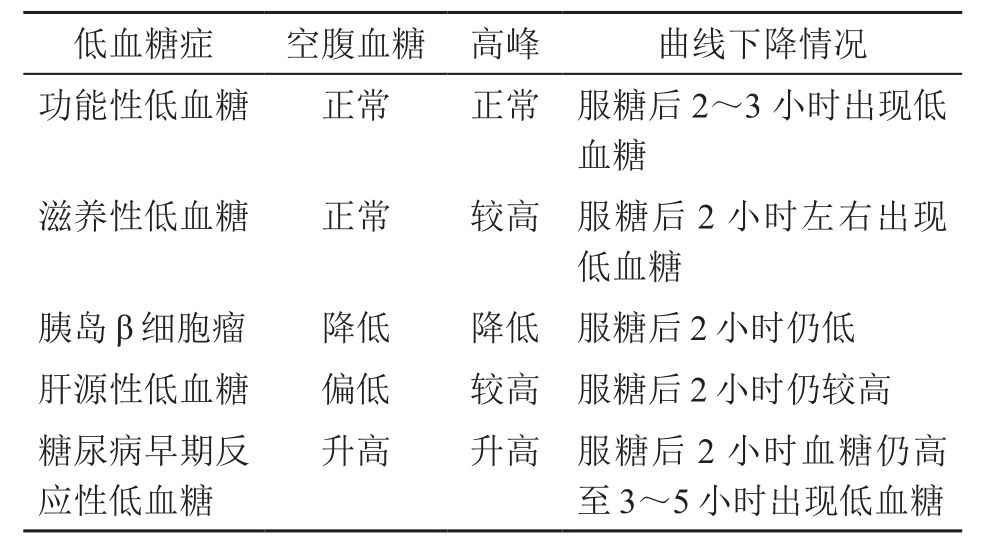
\includegraphics[width=3.27083in,height=1.84375in]{./images/Image00164.jpg}
\end{table}

\paragraph{血清胰岛素 、C肽、胰岛素原测定}

胰岛素测定在低血糖症的诊断中非常重要,尤其对内源性胰岛素分泌过多引起低血糖的诊断。由于胰岛素升高尚见于胰岛素抵抗、妊娠后期等。所以判断时必须结合同时测定的血糖值。①胰岛素释放指数:血浆免疫反应性胰岛素(μU/ml)与同时测定的血糖值(mg/dl)之比,正常<
0.3或> 0.4为异常,胰岛β细胞瘤的患者常>
1。②胰岛素释放修正指数:血浆胰岛素× 100/(血浆葡萄糖− 30mg/dl)。该值<
50为正常,> 80提示胰岛β细胞瘤。③低血糖时胰岛素测定值:放射免疫法>
6μU/ml或免疫化学发光法(ICMA)>
3μU/ml提示低血糖为胰岛素分泌过多所致。胰岛β细胞瘤患者的胰岛素水平很少超过100μU/ml(放免法),如超过1000mU/L提示为外源性胰岛素或存在胰岛素抗体。④C肽>
200pmol/L (ICMA)或胰岛素原>
5pmol/L(ICMA)也可以诊断为胰岛素分泌过多。

\paragraph{禁食试验}

正常人饥饿72小时血糖下降不< 3.1mmol/L,胰岛素不<
10μU/ml,而90\%胰岛β细胞瘤患者饥饿24小时内即有低血糖发作,发作时血糖<
2.5mmol/L而胰岛素水平不降,因而计算胰岛素释放指数增加。这项试验需在医生监护下进行,一旦出现低血糖症状,立即取血分测血糖和胰岛素,同时给患者注射葡萄糖或进食以终止试验。注意一次饥饿试验阴性不能完全排除胰岛素瘤。

\paragraph{激发试验}

是用药物加强和延长胰岛素分泌的刺激试验方法,有助于判断是否存在内源性胰岛素分泌过多。由于在胰岛β细胞瘤患者刺激试验有引起严重低血糖的危险,且有的患者无反应,临床诊断价值较低。临床多用于发作次数少、症状不典型及禁食试验无反应的疑难病例:

\hypertarget{text00120.htmlux5cux23CHP4-13-2-2-5-1}{}
(1) 甲苯磺丁脲刺激试验:

用甲苯磺丁脲钠1.0g溶于20ml注射用水中静脉推注,注射时间不能短于2分钟。注射后每5分钟测定一次血清胰岛素,持续15分钟,若胰岛素水平超过195μU/ml提示有胰岛素瘤存在。试验持续超过15分钟将会发现那些胰岛素延迟升高的胰岛素瘤患者,但可能会引起严重的低血糖。

\hypertarget{text00120.htmlux5cux23CHP4-13-2-2-5-2}{}
(2) 胰高血糖素刺激试验:

静脉注入1mg胰高血糖素,每5分钟测定一次血清胰岛素,连续15分钟。胰岛素水平超过135μU/ml提示有胰岛素瘤。当血清胰岛素过高时,胰高血糖素的升血糖作用作用可能较平常弱,但60分钟后可能接着出现严重的低血糖。

\paragraph{激素测定}

若由内分泌疾患引起的低血糖,根据不同的原因可测定生长激素、皮质醇、甲状腺激素、肾上腺素、性激素和IGF-Ⅰ、IGF-Ⅱ等。

\subsubsection{影像学检查}

影像学检查是定位诊断的主要手段,包括胰腺B超、CT、磁共振、选择性腹腔动脉血管造影、经皮肝门静脉插管测定激素法(PTPC)、选择性动脉钙刺激联合肝静脉取样、术前腹腔B超、内镜B超、术中B超等。世界范围报告显示各项定位检查的成功率为:CT
24\%,术前超声40\%,动脉造影43\%,经皮肝门静脉插管测定激素法(PTPC)88\%。结合检查费用和成功率,推荐首选超声检查,尤其是内镜B超或术中B超。因多数肿瘤太小(80\%<
2cm),故影像检查的阴性结果并不能排除诊断。有观点认为过多的术前定位检查并不必要,只要定性诊断明确,可直接由有经验的外科医生进行剖腹探查术,术中仔细探查配合IOUS(intraoperative
ultrasound)------“扪诊配合术中超声定位诊断”,可使肿瘤检出率达到95\%~100\%。

\subsubsection{诊断注意事项}

1.尚未确诊的低血糖昏迷
,应排除AEIOUH六大类昏迷原因,即:A.脑血管病;E.癫痫;I.感染;O.中毒;U.尿毒症;H.中暑。

2.已确诊低血糖症者,应与不同病因所致的低血糖症相鉴别。

(1)
糖尿病早期反应性低血糖:多在进食后3~5小时出现低血糖。患者多超重或肥胖,可有糖尿病家族史。5小时OGTT显示空腹血糖高于正常,服糖后0.5小时、1小时、2小时血糖升高,3~5小时可出现低血糖,血浆胰岛素高峰往往迟于血糖高峰。

(2) 特发性功能性低血糖症:为发生于餐后2~4小时或OGTT
2~5小时的暂时性低血糖。多见于女性,临床表现以肾上腺素分泌过多综合征为主,患者感心悸、心慌、出汗、面色苍白、饥饿、软弱无力、手足震颤、血压偏高等。一般无昏迷或抽搐,偶有昏厥、午餐及晚餐后较少出现。每次发作约15~20分钟,可自行缓解,病情非进行性发展,空腹血糖正常,发作时血糖可以正常或低至2.8mmol/L
(50mg/dl),但不会更低。口服葡萄糖耐量试验,在服糖后2~4小时其血糖可下降至过低值,然后恢复至空腹时水平。患者能耐受72小时禁食。没有胰岛素分泌过多的证据。糖尿病家族史常缺如。

(3)
肝源性低血糖:多有严重的肝脏疾患,肝功能异常。主要为空腹低血糖,饥饿、运动等可诱发出现,病情呈进行性。餐后可有高血糖。OGTT显示空腹血糖偏低,服糖后2小时血糖偏高,至3~5小时可能出现低血糖。

(4)
胰岛β细胞瘤:可见于任何年龄,女性约占60\%;起病缓慢,反复发作,进行性加重。多在清晨、饥饿及运动时发作低血糖,发作时血糖很低。OGTT呈低平曲线,血清胰岛素、C肽、胰岛素原浓度明显升高;禁食试验及激发试验均呈阳性反应。

(5)
酒精性低血糖:患者常有慢性肝病病史,在大量饮酒,尤其是空腹饮酒后出现低血糖;低血糖的临床表现常被醉酒状态所掩盖。没有胰岛素过多的证据;可伴有代谢性酸中毒、酮尿或酮血症。

(6)
胰外肿瘤:临床低血糖发作典型,多为空腹低血糖,有胰外肿瘤的依据、症状及体征。没有胰岛素分泌过多的证据,如血中IGF-Ⅱ增加有助于诊断。

(7)
胰岛素自身免疫综合征(IAS):常与其他自身免疫性疾病同时存在。实验室检查可发现低血糖的同时存在内源性胰岛素分泌过多的证据,血清中胰岛素自身抗体(IAA)阳性,少数可查出胰岛素受体抗体。

应注意低血糖危象,若以脑缺糖而表现为脑功能障碍为主者,可误诊为精神病、神经疾患(癫痫、短暂脑缺血发作)或脑卒中等。

3.确定低血糖危象 可依据Whipple三联征确定:①低血糖症状;②发作时血糖<
2.8mmol/L(50mg/dl);③补充葡萄糖后低血糖症状迅速缓解。少数空腹血糖降低不明显或处于非发作期的患者,应多次检测有无空腹或吸收后低血糖,必要时采用48~72小时禁食试验。

4.临床常用的词“低血糖反应”指有与低血糖相应的症状体征(主要是交感神经兴奋的表现),但血糖未低于2.8mmol/L,常见于药物治疗的糖尿病患者。“低血糖”则是一个生化诊断,指血糖低于2.8mmol/L的情况,往往伴有临床症状,无症状者称为“无症状低血糖”。患者没有自觉的前驱症状直接进入意识障碍状态者为“未察觉的低血糖症”(hypoglycemia
unawareness)。

\subsection{治疗}

低血糖危象为内科急症,如持续时间过长可使脑细胞不可逆损害以致脑死亡。因此应尽可能使血糖迅速恢复正常水平,防止低血糖的反复发作。

\subsubsection{急诊处理}

1.已明确低血糖危象而神志尚未完全丧失者,可给口服葡萄糖15~20g,同时采血测血糖浓度,每15分钟监测一次。

2.病情严重、神志不清者,立即静脉输入50\%葡萄糖20~60ml,通常10~15分钟后患者意识可以恢复。如效果不明显,可肌注胰高血糖素(成人1mg、儿童0.5mg),通常在10分钟内血糖即可升高。此后持续静脉滴注5\%~10\%葡萄糖液,根据病情调节葡萄糖液体量。血糖水平监测须追踪至少24~48小时。

3.如血糖恢复并维持正常水平后
,昏迷持续超过30分钟者,需考虑有脑水肿的可能。应加用20\%甘露醇液200ml或地塞米松10mg,根据情况再增减用量。

4.对胰岛素分泌过多所致的低血糖症可选择二氮嗪(氯甲苯噻嗪),其药理作用相似于氯噻嗪,但无利尿作用,有抑制胰岛素分泌作用,半衰期20~30小时。成人剂量200~600mg/d,儿童5~3mg/d。

\subsubsection{对症处理}

加强昏迷护理,对行为异常者要加强保护,以免出现意外,神志不清者可酌情加用抗生素,减少感染。垂体前叶功能低下或甲状腺功能低下引起的低血糖,应给予静滴氢化可的松或服用甲状腺素片。

\subsubsection{长期反复发作的低血糖}

此类患者的低血糖多为胰岛素瘤所致,应做手术切除;手术有禁忌证、拒绝手术以及术后未缓解或复发者,可服二氮嗪100~200mg/d,分2~3次服,与利尿剂合用可防止水潴留副作用。不能切除或已有转移的胰岛细胞癌,可用链脲佐菌素(streptozotocin),50\%的患者可缓解或延长存活时间。药物治疗同时应注意增加餐次,多吃含糖多脂的食物,必要时加用肾上腺皮质激素以防低血糖发作。胰岛素自身免疫综合征所引起的低血糖症,可服用泼尼松治疗。
\protect\hypertarget{text00121.html}{}{}

\chapter{糖尿病危象}

糖尿病(diabetes
mellitus,DM)是一组常见的以血糖水平增高为特征的代谢内分泌疾病,其基本病理生理变化是胰岛素绝对或相对分泌不足和胰高血糖素活性增高所引起的代谢紊乱,包括糖、蛋白质、脂肪、水及电解质等,严重时常导致酸碱平衡失常;其特征为高血糖、糖尿、葡萄糖耐量减低及胰岛素释放试验异常。临床上早期无症状,至症状期才有多食、多饮、多尿、烦渴、善饥、消瘦或肥胖、疲乏无力等症群,久病者常伴发心脑血管、肾、眼及神经等病变。严重病例或应激时可发生酮症酸中毒、高血糖高渗状态和乳酸性酸中毒等急性危象,若抢救及时,一般可以逆转,若延误诊治,死亡率均较高。因此,及早识别和诊断、正确处理这三类糖尿病危象是十分重要的。

糖尿病诊断是基于空腹血糖(FPG)、任意时间或口服葡萄糖耐量试验(OGTT)中2小时血糖值(2小时PG)。空腹指8~10小时内无任何热量摄入。任意时间指1日内任何时间,无论上一次进餐时间及食物摄入量。OGTT采用75g无水葡萄糖负荷。糖尿病症状指多尿、频渴多饮和难于解释的体重减轻。FPG
3.9~6.0mmol/L(70~108mg/dl)为正常;6.1~6.9mmol/L(110~125mg/dl)为空腹血糖调节受损(IFG);≥7.0mmol/L(126mg/dl)应考虑糖尿病。OGTT
2小时PG <
7.7mmol/L(139mg/dl)为正常糖耐量;7.8~11.0mmol/L(140~199mg/dl)为糖耐量减低(IGT);≥11.1mmol/L(200mg/dl)应考虑糖尿病。WHO(1999年)提出的并被我国糖尿病学会采纳的糖尿病诊断标准为:糖尿病症状加任意时间血浆葡萄糖≥11.1mmol/L(200mg/dl);或空腹血浆葡萄糖(FPG)≥7.0mmol/L(126mg/dl);或葡萄糖耐量试验(OGTT)中,2小时血浆葡萄糖≥11.1mmol/L
(200mg/dl)。

对于无糖尿病症状、仅一次血糖值达到糖尿病诊断标准者,必须在另一天复查核实而确定诊断。如复查结果未达到糖尿病诊断标准,应定期复查。IFG或IGT的诊断应根据3个月内的两次OGTT结果,用其平均值来判断。在急性感染、创伤或各种应激情况下可出现血糖暂时升高,不能以此诊断为糖尿病,应追踪随访。

关于糖尿病分型,目前国际上通用WHO糖尿病专家委员会提出的病因学分型标准(1999)。新的分类法将糖尿病分成四大类型,即1型糖尿病(T1DM)、2型糖尿病(T2DM)、其他特殊类型糖尿病和妊娠期糖尿病(GDM)。并取消胰岛素依赖型糖尿病(IDDM)和非胰岛素依赖型糖尿病(NIDDM)的医学术语;保留1、2型糖尿病的名称,用阿拉伯字,不用罗马字;糖耐量减低不作为一个亚型,而是糖尿病发展过程中的一个阶段;取消营养不良相关糖尿病。

\section{糖尿病酮症酸中毒}

糖尿病酮症酸中毒(diabetic
ketoacidosis,简称DKA)是由于体内胰岛素活性重度缺乏及升糖激素不适当增高,引起糖、脂肪和蛋白质代谢紊乱,以致水、电解质和酸碱平衡失调,出现高血糖、酮症,代谢性酸中毒和脱水为主要表现的临床综合征。是糖尿病的急性并发症,也是内科常见危象之一。当糖尿病代谢紊乱发展至严重阶段,脂肪分解加速,血清酮体积聚超过正常水平时称为酮血症,尿酮排出增多称为酮尿,此时临床表现统称酮症。酮体中酸基增多,大量消耗体内储备碱,而发生代谢性酸中毒,称为DKA;如病情严重发生昏迷时则称为糖尿病昏迷。

\subsection{病因与发病机制}

DKA的发生与糖尿病类型有关,与病程无关,约20\%以上新诊断的1型糖尿病和部分2型糖尿病患者可出现DKA。1型糖尿病有发生DKA的倾向,2型糖尿病在一定诱因下也可发生。在有的糖尿病患者,可以DKA为首发表现。DKA的临床发病大多有诱发因素,这些诱因多与加重机体对胰岛素的需要有关。常见的诱因有:①感染:是DKA最常见的诱因。常见有急性上呼吸道感染、肺炎、化脓性皮肤感染,胃肠道感染,如急性胃肠炎、急性胰腺炎、胆囊炎、胆管炎、腹膜炎等,以及泌尿道感染。②降糖药物应用不规范:由于体重增加、低血糖、患者依从性差等因素致使注射胰岛素的糖尿病患者,突然减量或终止治疗;或在发生急性伴发疾病的状态下,没有及时增加胰岛素剂量。③外伤、手术、麻醉、急性心肌梗死、心力衰竭、精神紧张或严重刺激引起应激状态等。④饮食失调或胃肠疾患,尤其是伴严重呕吐、腹泻、厌食、高热等导致严重失水和进食不足时,若此时胰岛素用量不足或中断、减量时更易发生。⑤妊娠和分娩。⑥胰岛素抗药性:由于受体和信号传递异常引起的胰岛素不敏感或产生胰岛素抗体,均可导致胰岛素的疗效降低。⑦伴有拮抗胰岛素的激素分泌过多,如肢端肥大症、皮质醇增多症或大量应用糖皮质激素、胰高血糖素、拟交感神经活性药物等。⑧糖尿病未控制或病情加重等。

胰岛素活性的重度或绝对缺乏和升糖激素过多(如胰高血糖素、儿茶酚胺类、皮质醇和生长激素)是DKA发病的主要原因。胰岛素缺乏和胰高血糖素升高是DKA发展的基本因素。胰岛素和胰高血糖素比率下降促进糖异生、糖原分解和肝酮体生成,肝的酶作用底物(游离脂肪酸、氨基酸)产生增加,导致高血糖、酮症和酸中毒。

\paragraph{酮症和酸中毒}

酮体包括β-羟丁酸、乙酰乙酸和丙酮。糖尿病加重时,胰岛素绝对缺乏,三大代谢紊乱,不但血糖明显升高,而且脂肪分解增加,脂肪酸在肝脏经β氧化产生大量乙酰辅酶A,由于糖代谢紊乱、草酰乙酸不足,乙酰辅酶A不能进入三羟酸循环氧化供能而缩合成酮体;同时由于蛋白合成减少,分解增加,血中成糖、成酮氨基酸均增加,使血糖、血酮进一步升高。β-羟丁酸、乙酰乙酸以及蛋白质分解产生的有机酸增加,循环衰竭、肾脏排出酸性代谢产物减少导致酸中毒。酸中毒可使胰岛素敏感性降低;组织分解增加,K\textsuperscript{+}
从细胞内逸出;抑制组织氧利用和能量代谢。严重酸中毒使微循环功能恶化,降低心肌收缩力,导致低体温和低血压。当血pH降至7.2以下时,刺激呼吸中枢引起呼吸加深加快;低至7.1~7.0时,可抑制呼吸中枢和中枢神经功能、诱发心律失常。

\paragraph{失水}

严重高血糖、高血酮和各种酸性代谢产物引起渗透压性利尿,大量酮体从肺排出又带走大量水分,厌食、恶心、呕吐使水分入量减少,从而引起细胞外失水;血浆渗透压增加,水从细胞内向细胞外转移引起细胞内失水。

\paragraph{电解质平衡紊乱}

渗透性利尿同时使钠、钾、氯、磷酸根等大量丢失,厌食、恶心、呕吐使电解质摄入减少,引起电解质代谢紊乱。胰岛素作用不足,物质分解增加、合成减少,钾离子(K\textsuperscript{+}
)从细胞内逸出导致细胞内失钾。由于血液浓缩、肾功能减退时K\textsuperscript{+}
滞留以及K\textsuperscript{+}
从细胞内转移到细胞外,因此血钾浓度可正常甚或增高,掩盖体内严重缺钾。随着治疗过程中补充血容量(稀释作用),尿量增加、K\textsuperscript{+}
排出增加,以及纠正酸中毒及应用胰岛素使K\textsuperscript{+}
转入细胞内,可发生严重低血钾,诱发心律失常,甚至心搏骤停。

\paragraph{携带氧系统失常}

红细胞向组织供氧的能力与血红蛋白和氧的亲和力有关,可由血氧离解曲线来反映。DKA时红细胞糖化血红蛋白(GHb)增加以及2,3二磷酸甘油酸(2,3-DPG)减少,使血红蛋白与氧亲和力增高,血氧离解曲线左移。酸中毒时,血氧离解曲线右移,释放氧增加(Bohr效应),起代偿作用。若纠正酸中毒过快,失去这一代偿作用,而血GHb仍高,2,3-DPG仍低,可使组织缺氧加重,引起脏器功能紊乱,尤以脑缺氧加重、导致脑水肿最为重要。

\paragraph{周围循环衰竭和肾功能障碍}

严重失水,血容量减少和微循环障碍未能及时纠正,可导致低血容量性休克。肾灌注量减少引起少尿或无尿,严重者发生急性肾衰竭。

\paragraph{中枢神经功能障碍}

严重酸中毒、失水、缺氧、体循环及微循环障碍可导致脑细胞失水或水肿、中枢神经功能障碍。此外,治疗不当如纠正酸中毒时给予碳酸氢钠不当导致反常性脑脊液酸中毒加重,血糖下降过快或输液过多过快、渗透压不平衡可引起继发性脑水肿并加重中枢神经功能障碍。

\subsection{诊断}

\subsubsection{病史与诱因}

有糖尿病病史或家族史,以及上述发病诱因。

\subsubsection{临床表现特点}

患者在出现明显DKA前,原有糖尿病症状加重如口渴、多饮、多尿、疲倦加重,并迅速出现食欲不振、恶心、呕吐、极度口渴、尿量剧增;常伴有头痛、嗜睡、烦躁、呼吸深快,呼气中含有烂苹果味。后期呈严重失水、尿量减少、皮肤干燥、弹性差、眼球下陷、脉细速、血压下降、四肢厥冷、反射迟钝或消失,终至昏迷。

由于DKA时心肌收缩力减弱、心搏出量减少,加以周围血管扩张、严重脱水、血压下降、周围循环衰竭。年长而有冠心病者可并发心绞痛、心肌梗死、心律不齐或心力衰竭等。

少数病例表现为腹痛(呈弥漫性腹痛),有的相当剧烈,可伴腹肌紧张、肠鸣音减弱或消失,极易误诊为急腹症。腹痛可能由于胸下部和上腹部辅助呼吸肌痉挛或因缺钾导致胃扩张和麻痹性肠梗阻所致;也可因肝脏迅速增大、DKA毒性产物刺激腹腔神经丛以及合并胰腺炎等所致;老年糖尿病患者出现腹痛和腹部体征时还应考虑与动脉硬化引起的缺血性肠病有关。

根据酸中毒的程度,可以将DKA分为轻度、中度和重度。轻度是指只有酮症,无酸中毒(糖尿病酮症);中度是指除酮症外,伴有轻~中度酸中毒(DKA);重度是指DKA伴意识障碍,或虽无意识障碍,但CO\textsubscript{2}
CP < 10mmol/L者。

\subsubsection{实验室检查}

\paragraph{血糖与尿糖}

血糖波动在11.2~112mmol/L(200~2000mg/dl),多数为16.7~33.3mmol/L(300~600mg/dl),有时可达55.5mmol/L(1000mg/dl)以上。如超过33.3mmol/L,应考虑同时伴有高血糖高渗状态或有肾功能障碍。尿糖强阳性,当肾糖阈升高时,尿糖减少甚至阴性。可有蛋白尿和管型。

\paragraph{血酮}

血酮体增高,定量一般>
4.8mmol/L(50mg/dl)。DKA时纠正酮症常比纠正高血糖缓慢。在DKA时,引起酸中毒作用最强、比例最高的是β-羟丁酸,而常用的亚硝酸铁氰化钠法仅仅可以测定乙酰乙酸和丙酮,无法检测β-羟丁酸。在治疗过程中,β-羟丁酸可以转化成乙酰乙酸,没有经验的医生可能误认为酮症恶化。因此监测DKA程度的最佳方法是直接测定β-羟丁酸。

\paragraph{尿酮}

当肾功能正常时,尿酮呈强阳性,但当尿中以β-羟丁酸为主时易漏诊(因亚硝酸铁氰化钠仅能与乙酰乙酸起反应,与丙酮反应较弱,与β-羟丁酸无反应)。肾功能严重损伤时,肾小球滤过率减少可表现为糖尿和酮尿减少甚至消失,因此诊断必须依靠血酮检查。若血pH明显降低而尿酮、血酮增加不明显者尚需注意有乳酸性酸中毒可能。

\paragraph{酸碱与电解质失调}

动脉血pH下降与血酮体增高呈平行关系,血pH≤7.1或CO\textsubscript{2} CP <
10mmol/L(< 20vol\%)时为重度酸中毒,血pH 7.2或CO\textsubscript{2} CP
10~15mmol/L为中度酸中毒,血pH > 7.2或CO\textsubscript{2} CP
15~20mmol/L为轻度酸中毒。血钠一般<
135mmol/L,少数正常,偶可升高达145mmol/L。血氯降低。血钾初期可正常或偏低,少尿而脱水和酸中毒严重期可升高至5mmol/L以上。血镁、血磷亦可降低。

\paragraph{血象}

血白细胞增多,无感染时可达(15~30)× 10\textsuperscript{9}
/L,尤以中性粒细胞增高较显著。血红蛋白、血细胞比容增高,反映脱水和血液浓缩情况。

\subsubsection{诊断注意事项}

早期诊断是决定治疗成败的关键,临床上对于原因不明的恶心呕吐、酸中毒、失水、休克、昏迷的患者,尤其是呼吸有酮味(烂苹果味)、血压低而尿量多者,不论有无糖尿病病史,均应想到本病的可能性。立即查末梢血糖、血酮、尿糖、尿酮,同时抽血查血糖、血酮、β-羟丁酸、尿素氮、肌酐、电解质、血气分析等以肯定或排除本病。如尿糖和酮体阳性,同时血糖增高,或血pH降低者,无论有无糖尿病病史即可诊断。DKA患者昏迷者只占少数,如发现有昏迷时尚应与糖尿病的另外几种危象情况相鉴别,详见表\ref{tab49-1}。

DKA患者可出现类似急腹症的临床表现,如呕吐、腹痛、腹部压痛与肌紧张、血白细胞增高等,与急腹症不易区别;急腹症患者也可因感染、呕吐不能进食而致酮症酸中毒,易与本症相混淆;而某些急腹症如急性胰腺炎、胆囊炎等有时可与DKA并存,使病情更为复杂。因此必须详询病史、细致的体检和必要的实验室检查,全面地加以分析判断。伴严重腹痛的DKA与急腹症的鉴别需注意以下特点:①病史:在疑似病例有时病史比体征更重要,若烦渴、多尿与厌食在腹部症状出现前早已存在,很可能患者全部临床表现是由DKA所致;如腹部症状较烦渴、多尿等症状出现为早,则急腹症的可能性较大。②体征:DKA时腹痛可急可缓,可伴有腹胀、腹部压痛,但反跳痛不明显,此种体征随酮症纠正很快改善;而急腹症时腹部压痛与反跳痛多明显,酮症纠正时,因病因未除去,临床症状不能好转。③腹痛特点:DKA时腹痛多呈弥散性,疼痛不固定,局限性压痛不明显;急腹症时均有相应的局限性压痛。

\subsection{治疗}

DKA的治疗原则是尽快补液以恢复血容量、纠正失水状态,降低血糖,纠正电解质及酸碱平衡失调,同时积极寻找和消除诱因,防治并发症,降低病死率。具体措施应根据病情轻重而定,如早期轻症,脱水不严重,酸中毒属轻度,无循环衰竭,神志清醒的患者,仅需给予足量正规胰岛素(RI),每4~6小时1次,每次皮下或肌肉注射10~20U,并鼓励多饮水,进半流汁或流汁饮食,必要时静脉补液,同时严密观察病情,随访尿糖、尿酮、血糖与血酮及CO\textsubscript{2}
CP、pH等,随时调整胰岛素量及补液量,并治疗诱因,一般均能得到控制,恢复到酮症前情况。对于中度和重症病例应积极抢救,具体措施如下。

\begin{table}[htbp]
\centering
\caption{糖尿病并发昏迷的鉴别}
\label{tab49-1}
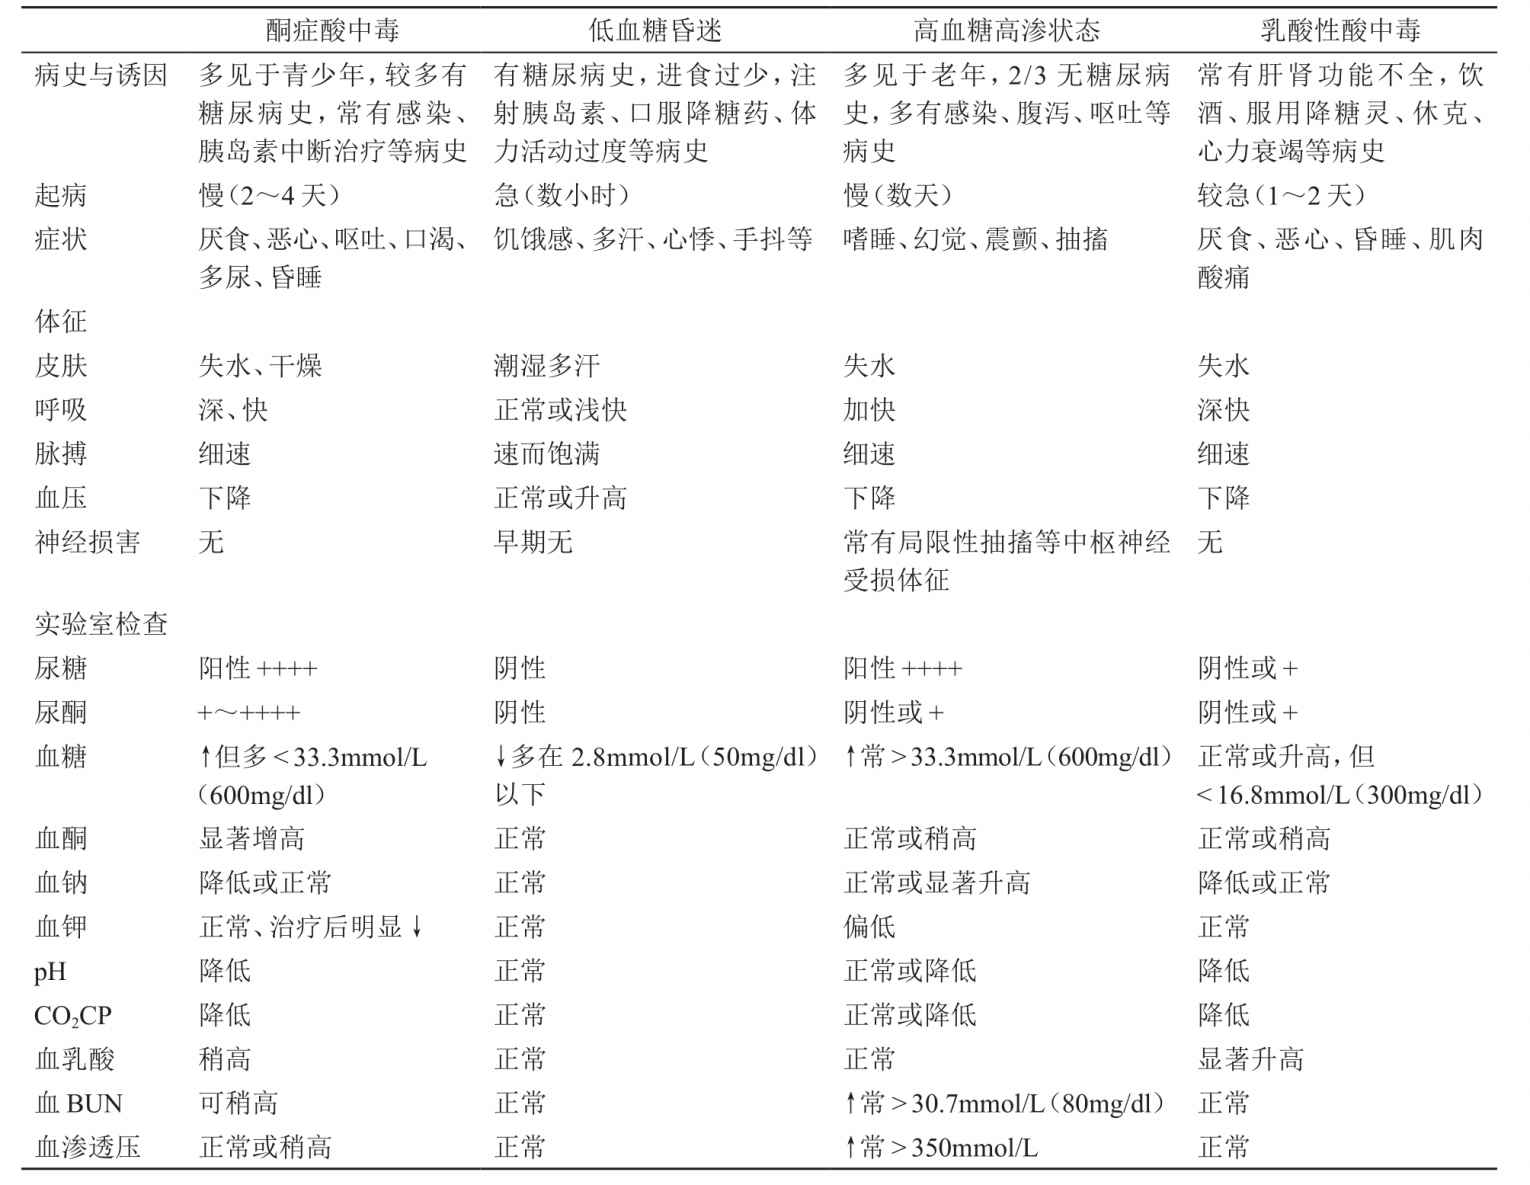
\includegraphics[width=6.6875in,height=5.17708in]{./images/Image00165.jpg}
\end{table}

\subsubsection{一般处理}

一般处理措施包括:①立即抽血验血糖、血酮体、钾、钠、氯、CO\textsubscript{2}
CP、BUN、血气分析等。②留尿标本,验尿糖与酮体、尿常规,计尿量;昏迷者应留置导尿管。③昏迷患者应保持呼吸道通畅,吸氧,注意保暖与口腔、皮肤清洁。④严密观察病情变化与细致护理:每1~2小时查血糖、电解质与CO\textsubscript{2}
CP(或血气分析)1次,直至血糖< 13.9mmol/L
(250mg/dl),CO\textsubscript{2} CP >
15mmol/L(33vol\%),延长至每4小时测1次。由于静脉pH比动脉pH降低0.03U,可以用静脉pH换算,从而减少反复动脉采血。

\subsubsection{补液}

补液是治疗的关键环节。只有在有效组织灌注改善、恢复后,胰岛素的生物效应才能充分发挥。可建立两条静脉输液通道:一条用作补液,另一条用作补充胰岛素。由于静脉内应用胰岛素需要保持一定的浓度和滴速,因此,保证胰岛素单独静脉通路是十分必要的。胰岛素是蛋白质,输注液体的pH、液体成分及输注物的分子量等因素均可能降低胰岛素的生物学效价,因此用于静脉滴注的胰岛素可以是生理盐水或葡萄糖溶液,尽量不与其他药物配伍。最初补液治疗的目的:①迅速扩张血管内外液体容量;②恢复肾脏血流灌注;③纠正高渗状态;④通过肾脏排泄酮体。早期以充分补充生理盐水为主,避免输入低渗液而使血浆渗透压下降过速,诱发脑水肿。补液总量可按患者体重的10\%估算。可建立两条静脉输液通道:一条用作补液,另一条用作补充胰岛素。补液宜先快后慢,头4小时内补总量的1/4~1/3;头8~12小时内补总量的2/3;其余部分在24~48小时内补给。补液时:①对无心功能不全者,头2小时输注生理盐水1000~2000ml;第3、4小时内各输入300~500ml;以后每4~6小时输入1000ml或更多,争取12小时内输入4000ml左右。第一个24小时输入总量约达4000~5000ml,严重失水者可达6000~8000ml。②已发生休克或低血压者,快速输液不能有效升高血压,应考虑输入胶体液如血浆、全血或血浆代用品等,并按需要给予其他抗休克治疗。对年老或伴有心脏病、心力衰竭者,应在中心静脉压监测下调节输液速度与输液量。③当血钠>
155mmol/L,又无心功能不全或休克时,可慎重考虑输入0.45\%低渗盐水1000~2000ml。待血糖降至13.9mmol/L(250mg/dl)时,改输5\%葡萄糖液,并按每2~4g葡萄糖加入1U
RI。同时减少输液量,防止低血糖反应。液体损失严重又持续呕吐者,可输入5\%葡萄糖盐水。

对无明显呕吐、胃肠胀气或上消化道出血者,可同时采取胃肠道补液。胃肠道补液的速度在头2小时内约500~1000ml,以后依病情调整。胃肠道补液量可占总补液量的1/3~1/2。考虑输液总量时,应包括静脉和胃肠道补液的总和。

\subsubsection{胰岛素治疗}

目前均釆用小剂量(短效)胰岛素疗法(每小时给予胰岛素0.1U/kg)。该方法具有简便、有效、安全,较少引起脑水肿、低血糖、低血钾等优点。且血清胰岛素浓度可恒定达到100~200μU/ml。这一血清胰岛素浓度已有抑制脂肪分解及酮体生成的最大效应,相当强的降低血糖的生物效应,而促进K\textsuperscript{+}
转运的作用则较弱。用药途径以持续静滴法最常用,以每小时0.1U/kg静滴维持(可用50U
RI加入生理盐水500ml中,以1ml/min的速度持续静滴)。对伴有昏迷和(或)休克和(或)严重酸中毒的重症患者,可加用首次负荷量胰岛素10~20U静脉注射。血糖下降速度一般每小时约降低3.9~6.1mmol/L(70~110mg/dl)为宜,每1~2小时复查血糖。若治疗2小时后血糖无肯定下降,提示患者对胰岛素敏感性降低,则将单位时间内的胰岛素剂量加倍,加大剂量后仍须继续定时检测血糖(1~2小时一次)。当血糖降至13.9mmol/L(250mg/dl)时,可改用5\%葡萄糖液500ml加RI
6~12U(即1U胰岛素:2~4g葡萄糖)持续静滴,胰岛素滴注率下调至0.05U/(kg•h),此时仍需每4~6小时复查血糖。当血糖降至11.1mmol/L以下,血
,血pH >
7.3,尿酮体转阴后,可以开始
\includegraphics[width=1.02083in,height=0.16667in]{./images/Image00166.jpg}
皮下注射胰岛素方案。但应在停静滴胰岛素前1小时皮下注射一次RI,一般注射量为8U以防血糖回跳。其他用药途径可采用间歇肌肉注射或间歇静脉注射,每小时注射1次,剂量仍为0.1U/kg。

DKA临床纠正的标准为:血糖<
11.1mmol/L(200mg/dl),血
\includegraphics[width=0.96875in,height=0.15625in]{./images/Image00167.jpg}
,静脉血pH > 7.3。

\subsubsection{纠正电解质和酸碱平衡失调}

据估计一般较重病例可失钠500mmol、钾300~1000mmol、氯350mmol、钙及磷各50~100mmol、镁25~

50mmol、,
失水约5.6L,故补液中应
\includegraphics[width=1.20833in,height=0.16667in]{./images/Image00168.jpg}
注意补充此损失量。当开始补生理盐水后钠、氯较易补足。

\paragraph{纠正低血钾}

DKA患者体内总缺钾量通常达300~1000mmol,但在治疗前,细胞内的K\textsuperscript{+}
大量转移到细胞外液,再加上失水、血液浓缩、肾功能减退等因素,血钾不仅不降低,有时反显增高,因此,治疗前血钾水平不能真实反映体内缺钾程度。治疗开始后因胰岛素发挥作用,大量钾转入细胞内,大量补液致血液浓缩改善,加上葡萄糖对肾脏渗透效应致钾与钠进一步丢失,治疗后4小时左右血钾常明显下降,有时达严重程度。因此,不论患者开始时血钾是否正常或略升高,在使用胰岛素4小时后,只要患者有尿排出(≥30ml/h),便应给予静脉补钾。如治疗前血钾水平已低于正常,开始治疗时即应补钾;如治疗前血钾正常,尿量≥40ml/h,可在输液和胰岛素治疗的同时即开始补钾;若尿量<
30ml/h,宜暂缓补钾,待尿量增加后即开始补钾。血钾<
3mmol/L时,每小时补钾26~39mmol(氯化钾2~3g);血钾3~4mmol/L时,每小时补钾20~26mmol(氯化钾1.5~2.0g);血钾4~5mmol/L时缓慢静滴,每小时补钾6.5~13mmol/L(氯化钾0.5~1.0g);血钾>
5.5mmol/L时应暂缓补钾。有条件时应在心电监护下,结合尿量与血钾水平,调整补钾量与速度。神志清醒者可同时口服钾盐。由于钾随糖、镁、磷等进入细胞较慢,补钾须继续5~7天方能纠正钾代谢。经充分补钾2~3天后低血钾难以纠正,或血镁<
0.72mmol/L(1.8mg/dl)时,应考虑补镁。用10\%~25\%硫酸镁1~2g肌肉注射,或加入液体中静滴;亦可用门冬氨酸钾镁20~60ml加入液体中滴注。

\paragraph{纠正酸中毒}

轻症患者经补液及胰岛素治疗后,钠丧失和酸中毒可逐渐得到纠正,不必补碱。重症酸中毒使外周血管扩张和降低心肌收缩力,导致低体温和低血压,并降低胰岛素敏感性,抑制呼吸中枢和中枢神经系统功能,故应给予相应治疗。但酮症酸中毒的基础是酮酸生成过多,非{}
损失过多;故必须采用胰岛素抑制酮体生成,促进酮体氧化,且酮体氧化后产生
\includegraphics[width=1.03125in,height=0.15625in]{./images/Image00170.jpg}
30vol\%),无明显酸中毒大呼吸者可不予补碱或停止补碱。

\subsubsection{消除诱因与防治并发症}

\paragraph{抗感染}

感染既可作为诱因,又是DKA的常见并发症,应积极抗感染治疗。

\paragraph{防治并发症}

包括休克、心力衰竭、心律失常、肾功能不全、脑水肿等,详见有关章节。

\protect\hypertarget{text00122.html}{}{}

\section{高血糖高渗状态}

高血糖高渗状态(hyperglycemic hyperosmolar
state,HHS)是糖尿病急性代谢紊乱的另一临床类型。以严重高血糖、高血浆渗透压、脱水为特点,无明显酮症酸中毒,患者常有不同程度的意识障碍或昏迷。HHS与既往所称的“高渗性非酮症糖尿病昏迷”(hyperosmolar
nonketotic diabetic coma,HNDC)、高渗性昏迷(hyperosmolar
coma)略有不同,因为部分患者并无昏迷,部分患者可伴有酮症。与DKA相比,HHS失水更为严重,神经精神症状更为突出。本症多见于老年患者,好发年龄为50~70岁,但各年龄组均可发病,男女发病率大致相同。临床特点为无明显酮症与酸中毒,血糖显著升高,严重脱水甚至休克,血浆渗透压增高,以及进行性意识障碍等。

\subsection{病因与发病机制}

HHS的基本病因与DKA相同,但值得注意的是约2/3HHS患者发病前无糖尿病史,或者不知有糖尿病,有糖尿病史者也多为轻症2型糖尿病,偶也可发生于年轻的1型糖尿病患者。HHS除了原有的糖尿病基础外,几乎都有明显的诱发因素,临床上常见的诱因包括:①应激:如感染(尤其是呼吸道与泌尿道感染)、外伤、手术、急性脑卒中、急性心肌梗死、急性胰腺炎、胃肠道出血、中暑或低温等;②摄水不足:可见于口渴中枢敏感性下降的老年患者,不能主动进水的幼儿或卧床患者、精神失常或昏迷患者,以及胃肠道疾病患者等;③失水过多:见于严重的呕吐、腹泻,以及大面积烧伤患者等;④药物:如各种糖皮质激素、利尿剂(特别是噻嗪类和呋塞米)、苯妥英钠、氯丙嗪、普萘洛尔、西咪替丁、免疫抑制剂等;⑤高糖的摄入:见于大量服用含糖饮料、静脉注射高浓度葡萄糖、完全性静脉高营养,以及含糖溶液的血液透析或腹膜透析等。有时在病程早期因误诊而输入大量葡萄糖液或因口渴而摄入大量含糖饮料可诱发本病或使病情恶化。上述诸因素均可使机体对胰岛素产生抵抗、升高血糖、加重脱水,最终诱发或加重HHS的发生与发展。

HHS是体内胰岛素相对缺乏使血糖升高,并进一步引起脱水,最终导致的严重高渗状态。胰岛素相对不足、液体摄入减少是HHS的基本病因。胰岛素缺乏促进肝葡萄糖输出(通过糖原分解和糖异生)、损伤了骨骼肌对葡萄糖的利用,高血糖的渗透性利尿作用导致血容量不足,如补液不充分,患者病情加重。另外,HHS的发生发展受到一系列因素的影响:存在感染、外伤、脑血管意外等诱发因素的情况下,胰岛素分泌进一步减少,对抗胰岛素的激素水平升高,血糖明显升高;HHS多发生于老年患者,口渴中枢不敏感,加上主动饮水的欲望降低和肾功能不全,失水常相当严重,而钠的丢失少于失水,致血钠明显增高;脱水和低血钾一方面能引起皮质醇、儿茶酚胺和胰高血糖素等升糖激素的分泌增多,另一方面进一步抑制胰岛素分泌,继而造成高血糖状态的继续加重,形成恶性循环,最终导致HHS发生。

HHS与DKA都是由于胰岛素缺乏而引起的糖尿病急性并发症,DKA主要表现为高血糖、酮症和酸中毒,而HHS以严重高血糖和高渗透压为特征。这两种代谢紊乱临床表现的差别,可能的原因为:①HHS时胰岛素只是相对缺乏,分泌的胰岛素虽足以抑制脂肪分解和酮体生成,但却不能抑制糖异生,故主要为血糖的明显升高;但在DKA胰岛素是高度缺乏,已不能抑制酮体生成;②胰高血糖素等升糖激素升高较轻,促进脂肪分解和生酮作用较弱;③HHS时失水严重,不利于酮体产生;④部分HHS患者血浆非酯化脂肪酸水平高而无酮症,提示肝生酮功能障碍;⑤严重高血糖和酮体生成之间可能存在拮抗作用。由此可见,HHS与DKA是不同程度的胰岛素缺乏所导致的两种状态,两者可能同时存在,实际上,1/3的高血糖患者可同时表现出HHS和DKA的特征。

\subsection{诊断}

\subsubsection{病史}

患者多为老年人,部分患者已知有糖尿病,30\%患者有心脏疾病,90\%患者有肾脏病变。可有诱发疾病如肺炎、泌尿系感染、胰腺炎等的表现。

\subsubsection{临床表现特征}

\paragraph{前驱期特点}

HHS起病多隐蔽,在出现神经系统症状至进入昏迷前常有一段时间,即前驱期,时间一般为1~2周。表现为糖尿病症状如口渴、多尿和倦怠、乏力等症状的加重,反应迟钝,表情淡漠,引起这些症状的基本原因是由于渗透性利尿脱水。若能对本症提高警惕,在前驱期及时发现并诊断,则对患者的治疗和预后大有好处。但由于前驱期症状无特异性易被患者本人和医生所忽略,且常被其他合并症症状所掩盖和混淆,致使诊断困难和延误。

\paragraph{典型期的表现}

如前驱期得不到及时诊治,则病情继续发展,主要表现为严重的脱水和神经系统两组症状和体征。脱水表现为皮肤干燥和弹性减退,眼球凹陷、唇舌干裂、脉搏快而弱,卧位时颈静脉充盈不好,立位时血压下降。严重者出现休克,但因脱水严重,体检时可无冷汗。有些患者虽有严重脱水,但因血浆的高渗促使细胞内液外出,并补充了血容量,可能掩盖了失水的严重程度,而使血压仍保持正常。神经系统方面则表现为不同程度的意识障碍,从意识模糊、嗜睡直至昏迷。HHS患者的意识障碍与否,主要决定于血浆渗透压升高的程度与速度,与血糖的高低也有一定关系,而与酸中毒的程度关系不大。通常患者血浆有效渗透压>
320mOsm/L时,即可出现精神症状,如淡漠、嗜睡等;而当患者血浆有效渗透压>
350mOsm/L时,可有定向力障碍、幻觉、上肢拍击样粗震颤、癫痫样发作、偏瘫、偏盲、失语、视觉障碍、昏迷和阳性病理征等,这些提示患者可能有因脱水、血液浓缩和血管栓塞而引起的大脑皮质或皮质下的损害。出现神经系统症状常是促使患者前来就诊的原因,因此常被误诊为一般的脑卒中等颅内疾病而导致误诊误治,后果严重。和酮症酸中毒不一样,HHS没有典型的酸中毒大呼吸,如患者出现中枢性过度换气现象时,则应考虑是否合并有脓毒症和脑卒中。

\subsubsection{实验室检查}

\paragraph{血常规}

由于脱水血液浓缩,血红蛋白增高,白细胞计数多> 10 ×
10\textsuperscript{9} /L。

\paragraph{尿检查}

尿糖多强阳性,患者可因脱水及肾功能损害而致尿糖不太高,但尿糖阴性者罕见。尿酮体多阴性或弱阳性。

\paragraph{血糖}

常≥33.3mmol/L,一般为33.3~66.6mmol/L
(600~1200mg/dl),有高达138.8mmol/L(2500mg/dl)或更高者。血酮体多正常。另外,因血糖每升高5.6mmol/L,血钠下降1.6mmol/L左右,HHS时存在严重高血糖,可造成血钠水平假性降低。

\paragraph{血尿素氮(BUN)和肌酐(Cr)}

常显著升高,反映严重脱水和肾功能不全。BUN可达21~36mmol/L(60~100mg/dl),Cr可达124~663μmol/L(1.4~7.5mg/dl),BUN/Cr比值(按mg/dl计算)可达30∶1(正常人多在10~20∶1)。有效治疗后BUN及Cr多显著下降。BUN与Cr进行性升高的患者预后不佳。

\paragraph{血浆渗透压}

显著升高,多超过350mOsm/L,有效渗透压超过320mOsm/L。血浆渗透压可直接测定,也可根据血糖及电解质水平进行计算,公式为:血浆渗透压(mOsm/L)=
2({[}Na\textsuperscript{+} {]}+{[}K\textsuperscript{+}
{]})+血糖(mmol/L)+ BUN
(mmol/L),正常值为280~300mOsm/L;若BNU不计算在内,则为有效渗透压,因BUN可自由进出细胞膜。

\paragraph{电解质}

血Na\textsuperscript{+} 可升高>
145mmol/L,也可正常或降低。血K\textsuperscript{+}
正常或降低,有时也可升高。血Cl\textsuperscript{−}
情况多与Na\textsuperscript{+} 一致。血Na\textsuperscript{+}
、Na\textsuperscript{+} 、Cl\textsuperscript{−}
的水平取决于其丢失量,在细胞内外的分布情况及患者的血液浓缩程度。不论其血浆水平如何,患者总体Na\textsuperscript{+}
、K\textsuperscript{+} 、Cl\textsuperscript{−}
都是丢失的。有人估计,HHS患者Na\textsuperscript{+}
、K\textsuperscript{+} 和Cl\textsuperscript{−}
丢失分别为5~10mmol/kg、5~15mmol/kg和5~7mmol/kg。此外,还可有Ca\textsuperscript{2+}
、Mg\textsuperscript{2+} 和磷的丢失。

\paragraph{酸碱平衡}

约半数患者有轻、中度代谢性酸中毒,pH多高于7.3,{} 常高于15mmol/L。

\subsubsection{诊断注意事项}

HHS的病死率仍较高,能否及时诊断直接关系到患者的治疗和预后。从上述其临床表现来看,本症的诊断并不困难,关键是临床医生要提高对本症的警惕和认识,特别是对中、老年患者有以下临床情况者,无论其有无糖尿病病史,均应考虑有HHS的可能,应立即作实验室检查:①进行性意识障碍和明显脱水表现者;②中枢神经系统症状和体征,如癫痫样抽搐和病理反射征阳性者;③合并感染、心肌梗死、手术等应激情况下出现多尿者;④大量摄糖,静脉输糖或应用激素、苯妥英钠、普萘洛尔等可致血糖增高的药物时出现多尿并有意识改变者;⑤昏迷休克患者,休克未曾纠正而尿量多者。

HHS的诊断依据是:①中、老年患者,血糖≥33.3mmol/L
(600mg/dl);②有效渗透压≥320mOsm/L;③动脉血气分析示pH≥7.30或血{}
浓度≥15mmol/L;④尿糖强阳性,血酮体阴性或弱阳性。但应值得注意的是HHS有并发DKA或乳酸性酸中毒的可能性。个别病例的高渗状态主要是由于高血钠,而不是高血糖造成的。因此尿酮体阳性,酸中毒明显或血糖<
33.3mmol/L,并不能作为否定HHS诊断的依据。但HHS患者无一例外地存在明显的高渗状态,如昏迷患者血浆有效渗透压<
320mOsm/L,则应考虑到糖尿病并发其他急性并发症的可能性(参见表\ref{tab49-1})。

\subsection{治疗}

HHS的基本病理生理改变是高血糖、高渗透压引起脱水、电解质丢失和血容量不足,以致患者休克和肾、脑组织脱水与功能损害,而危及患者的生命。因此,其治疗原则是立即补液,使用胰岛素、纠正电解质紊乱和防治并发症,与DKA基本相同。

\subsubsection{补液}

HHS患者均有严重脱水,而高渗状态引起的脑细胞脱水是威胁患者生命的主要原因,单纯补液即可使血糖每小时下降1.1mmol/L(20mg/dl),可使血浆渗透压下降,减轻脑细胞水肿。因此,迅速补液以恢复血容量,纠正高渗和脱水是抢救成败的关键。本症患者脱水比DKA严重,失水量多在发病前体液的1/4或体重的1/8以上。补液时可根据患者的脱水程度,按其体重的10\%~15\%估算;也可以按血浆渗透压计算患者的失水量,计算公式为:患者的失水量(L)=(患者血浆渗透压−
300)÷ 300(为正常血血浆渗透压)×体重(kg)×
0.6。考虑到在治疗过程中将有大量液体自肾脏、呼吸道及皮肤丢失,补液总量可略高于估计的失液总量。一般在最初2小时可补液1000~2000ml,头4小时内输入补液总量的1/3,头12小时内补入总量的1/2加尿量,其余在以后24小时内补足。经积极补液4~6小时后仍少尿或无尿者,宜给呋塞米(速尿);若发现有显著的肾损害,则输液量要适当调整。在静脉输液的同时,应尽可能通过口服或胃管进行胃肠道补液,此法有效而且简单和安全,可减少静脉补液量,从而减轻大量静脉输液引起的副作用。在输液中,应注意观察患者的尿量、颈静脉充盈度并进行肺部听诊,有条件时应行中心静脉压监测,以指导补液。

补液后细胞脱水状态改善,葡萄糖利用率提高,肾功能改善,排糖能力增强,继而产生抗胰岛素水平下降等效应,可使血糖明显下降。一般每输入1500ml液体可使血糖降低18\%,但在有肾实质病变的患者充足补液尚不能恢复正常的排糖功能,血糖下降缓慢。

关于补液的种类和浓度,目前多主张治疗开始时用等渗盐水(308mmol/L),因大量输入等渗液不会引起溶血,有利于恢复血容量,纠正休克,改善肾血流量,恢复肾脏调节功能。休克患者应另予血浆或全血。如无休克或休克已纠正,在输入生理盐水1000~2000ml后,血浆渗透压仍>
350mOsm/L,血钠>
155mmol/L时,可考虑输入适量低渗液如0.45\%氯化钠溶液(154mmol/L)或2.5\%葡萄糖溶液(139mmol/L)。当血浆渗透压降至330mOsm/L时再改为等渗液。在治疗过程中,当血糖下降至16.7mmol/L(300mg/dl),应使用5\%葡萄糖液(278mmol/L)或5\%葡萄糖盐水(586mmol/L),并酌情加用胰岛素,以防止血糖及血浆渗透压过快下降。应注意:5\%葡萄糖液的渗透压为278mOsm/L,虽为等渗,但糖浓度约为正常血糖的50倍,5\%葡萄糖盐水的渗透压为586mOsm/L,在治疗早期两者均不适用,以免加重高血糖、高血钠及高渗状态。停止补液的条件是:①血糖<
13.9mmol/L(250mg/dl);②尿量>
50ml/h;③血浆渗透压降至正常或基本正常;④患者能饮食。

\subsubsection{胰岛素治疗}

其使用原则与方法和DKA大致相同,即在输液开始时同时给予小剂量胰岛素静脉滴注。HHS患者一般对胰岛素比DKA敏感,在治疗中对胰岛素需要量相对较少。经输液和用胰岛素后血糖降至≤16.7mmol/L(300mg/dl)、血浆渗透压下降至<
330mOsm/L时,将液体改为5\%葡萄糖液,同时按2~4g葡萄糖:1U胰岛素的比例加入胰岛素静滴(详见DKA的治疗),若此时血钠仍低于正常则宜用5\%葡萄糖盐水。在补充胰岛素时,应注意高血糖是维护患者血容量的重要因素,如血糖降低过快而液体又补充不足,将导致血容量和血压进一步下降,反而促使病情恶化。因此,应使血糖每小时以2.75~3.9mmol/L(50~70mg/dl)的速度下降,尿糖保持在“+~++”为宜。

\subsubsection{纠正电解质紊乱}

与DKA治疗相同。

\subsubsection{防治并发症}

各种并发症特别是感染,常是患者晚期死亡的主要原因,必须一开始就给予大剂量有效的抗生素治疗。其他并发症的治疗如休克、肾功能不全、心力衰竭等,参见有关章节。

\subsubsection{其他措施}

包括去除诱因、支持疗法和对症处理等。

\protect\hypertarget{text00123.html}{}{}

\section{乳酸性酸中毒}

乳酸性酸中毒(lactic
acidosis,LA)是由于各种原因导致组织缺氧,乳酸生成过多,或由于肝脏病变致使乳酸利用减少,清除障碍,血乳酸浓度明显升高引起。本症是糖尿病的急性并发症之一,多发生于伴有全身性疾病或大量服用双胍类药物的患者。可单独存在或与酮症酸中毒和高血糖高渗状态并存,其病情严重,病死率高达50\%以上,早期诊断与治疗非常重要。

\subsection{病因与发病机制}

乳酸是糖无氧酵解的终产物,在供氧正常时放出能量ATP,但当供氧不足时,丙酮酸不能进一步代谢而堆积在细胞内,在乳酸脱氢酶系的作用下,丙酮酸由NADH(还原型辅酶Ⅰ)获得H\textsuperscript{+}
而转变为乳酸,正常乳酸的产生与利用之间保持平衡,血乳酸浓度正常值为0.4~1.4mmol/L,约为丙酮酸的10倍。当全身或局部缺血、缺氧在细胞水平氧利用减低,糖酵解增强,丙酮酸生成增多,直接转变为乳酸也越多。随着血乳酸生成,血pH改变取决于:①组织产生乳酸的速度;②细胞外液的缓冲能力;③肝、肾对H\textsuperscript{+}
清除的能力。因此血乳酸堆积有两种情况,一种只是血乳酸水平暂时增加而无血pH降低的“高乳酸血症”(hyperlactacidemia),即Huckabee分型Ⅰ型;另一为乳酸性酸中毒,血乳酸增高同时有H\textsuperscript{+}
堆积、血pH降低,即Huckabee分型Ⅱ型。Ⅱ型按不同的病因机制又分为两个亚型:A型也叫“继发性乳酸性酸中毒”,继发于各种缺氧或缺血性疾病,如各种休克时。其发病机制是组织获得的氧不能满足组织代谢需要,导致无氧酵解增加,产生A型乳酸性酸中毒;B型也称“自发性乳酸性酸中毒”,因肝、肾疾病及白血病等全身性疾病以及某些药物(如苯乙双胍)引起乳酸代谢障碍所致。其发病机制与组织缺氧无关。B型可进一步分为三种亚型:B\textsubscript{1}
型与糖尿病、脓毒血症、肝肾功能衰竭等常见病有关;B\textsubscript{2}
型与药物或毒素有关;B\textsubscript{3}
型与肌肉剧烈活动、癫痫发作等其他因素有关。糖尿病乳酸性酸中毒常发生于2型糖尿病,其虽与上述各型都有联系,但更常见的是由口服双胍类降糖药(苯乙双胍即降糖灵,二甲双胍)引起的。苯乙双胍(DBI)引起乳酸性酸中毒的原因是:①DBI增加糖无氧酵解使乳酸产生增加;②减少了肝和肌肉对乳酸的摄取;③减少了肾脏排酸功能。已证实二甲双胍升高血乳酸的能力较DBI小,因而已逐渐代替DBI。过量饮酒、超量应用胰岛素等都有诱发乳酸性酸中毒的可能。另外,亦与糖尿病患者已合并有慢性心、肺疾病或肝、肾功能障碍有关。

\subsection{诊断}

\subsubsection{临床表现特点}

LA多见于50岁以上2型糖尿病,使用双胍类降糖药的过程中或伴发于急性重症并发症时。起病较急,主要表现为代谢性酸中毒引起的大呼吸,严重时神志模糊、精神恍惚、谵妄至昏迷,也可出现呕吐、腹泻等脱水症状,可有明显的腹痛,易误诊为急腹症。其临床过程又不能以肾功能衰竭或酮症酸中毒解释。

\subsubsection{实验室检查}

实验室检查是乳酸性酸中毒诊断的关键。除糖尿病的实验室检查外,还有:①血酸度明显增高:血pH
< 7.30,有的可降至7.0以下;血{} 明显降低,常< 10mmol/L。②血乳酸:常>
5mmol/L,有时可达35mmol/L(>
25mmol/L者大多不治);血丙酮酸相应增高,达0.2~1.5mmol/L;血乳酸/丙酮酸≥30。当乳酸浓度>
5mmol/L,HCO\textsubscript{3} \textsuperscript{−}
≤10mmol/L,乳酸/丙酮酸>
30而可除外其他酸中毒原因时,可确诊为本病。③血浆阴离子间隙(AG)∶AG常>
18mmol/L,可达25~45mmol/L(正常值12~16mmol/L)。AG增高常见于糖尿病酮症酸中毒或酒精性酮症酸中毒、尿毒症性酸中毒、乳酸性酸中毒及某些药物毒性所致如水杨酸盐等,临床上若排除前两者,又不存在药物毒性的可能,此时AG增高强烈支持乳酸性酸中毒。④血酮体一般不升高,或轻度升高。

\subsubsection{诊断注意事项}

糖尿病患者在服用双胍类降糖药过程中,呈现严重酸中毒,既无酮体增多(血酮、尿酮皆不增多),又无严重高血糖、血浆渗透压增高或高血钠等,即应疑及本症。凡有休克、缺氧、肝肾功能衰竭者,如酸中毒较重时,必须警惕LA的可能性。确诊依靠血乳酸测定,若无乳酸测定的设备条件,可根据AG增大,但先决条件是除外酮症酸中毒及高血糖高渗状态,其鉴别详见表\ref{tab49-1}。LA主要诊断标准为:①血乳酸≥5mmol/L;②动脉血pH≤7.35;③AG
> 18mmol/L;④{} < 10mmol/L;⑤CO\textsubscript{2}
CP降低;⑥丙酮酸增高,乳酸/丙酮酸≥30∶1;⑦血酮体一般不升高。

\subsection{防治}

\paragraph{预防为主}

LA病死率高,治疗难度大,故必须提高警惕,认真预防。双胍类药物如DBI可诱发LA,肝、肾、心功能不全时,可导致双胍类药物在体内蓄积,因此在应用双胍类药物前应查肝、肾、心功能,若存在功能不全则忌用双胍类药物。对于其他能诱发LA的药物,如水杨酸、异烟肼、山梨醇、乳糖等,也应尽量避免应用。休克、缺氧、肝肾功能衰竭状态下的危重患者,若伴有酸中毒,须警惕发生LA的可能性,并努力防治。

\paragraph{一般措施}

寻找和去除诱发LA的诱因,停用所有可诱发LA的药物与化学物质,有利于B型LA的治疗。畅通呼吸道,充分供氧,改善氧合功能。并加强监测。

\paragraph{纠正休克}

是治疗A型LA的重要措施。补液扩容可改善组织灌注,减少乳酸的产生,促进利尿排酸。输液宜用生理盐水,避免用含乳酸的液体。

\paragraph{纠正酸中毒}

高渗碳酸氢钠溶液可抑制HbO\textsubscript{2}
分离,加重组织缺氧,尤其有早期循环衰竭者;大剂量碳酸氢钠可引起血钠过高、血渗透压升高、容量负荷加重,血乳酸反而增高。故目前主张用小剂量等渗碳酸氢钠溶液持续静脉滴注的方式,使{}
上升4~6mmol/L,维持在14~16mmol/L,动脉血pH升至7.2。

缺乏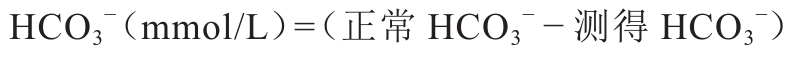
\includegraphics[width=2.66667in,height=0.17708in]{./images/Image00176.jpg}
(mmol/L)× 0.5 ×体重(kg)。

糖尿病患者有DKA存在时仅需少量碳酸氢钠使pH恢复到7.0~7.1为宜。除补液补碱外,随时补充钾盐以防低钾或缺钾。

\paragraph{降低血乳酸}

①胰岛素治疗:胰岛素不足是导致糖尿病LA的诱因之一。胰岛素不足使丙酮酸脱氢酶活性降低,丙酮酸进入三羧酸循环减少。应用胰岛素治疗,减少糖无氧酵解,有利于血乳酸的清除。血糖不高的患者需同时静滴葡萄糖液。②亚甲蓝(美蓝):为氧化还原剂,其作用类似NAD\textsuperscript{+}
,可促使乳酸转化为丙酮酸,降低血乳酸的浓度。用法是1~5mg/kg静滴,2~6小时作用达高峰,可维持14小时。③二氯醋酸(dichloroacetate,DCA):是丙酮酸脱氢酶激活剂,能迅速增强乳酸的代谢,并可阻止肝细胞释放乳酸和丙酮酸,使血中浓度进一步降低。此外,DCA能增强心肌收缩力和心输出量,从而改善心脏灌注,明显提高患者生存水平。④血液净化疗法:用不含乳酸钠的透析液进行血液或腹膜透析治疗,可加速乳酸排泄,并可清除DBI等引起LA的药物,尤其适用于不能耐受钠过多的老年患者与肾功能衰竭患者,对双胍类药物引起的LA是最为有效的治疗方法。
\protect\hypertarget{text00124.html}{}{}

\hypertarget{text00124.htmlux5cux23CHP4-14-4}{}
参 考 文 献

1. 陆再英,钟南山.内科学.第7版.北京:人民卫生出版社,2008:770

2. 王姮 ,杨永年.糖尿病现代治疗学.北京:科学出版社,2005:265

3. 陈灏珠 ,林果为.实用内科学.第13版.北京:人民卫生出版社,2009:1018

4. Kitabchi AE,Umpierrez GE,Murphy MB,et al. Management of
hyperglycemic crises in patients with diabetes. Diabetes
Care,2001,24:131

5.
中华医学会糖尿病学分会.中国2型糖尿病防治指南.中华内分泌代谢杂志,2008,24(2):增录

\protect\hypertarget{text00125.html}{}{}

\chapter{痛 风 危 象}

高尿酸血症(hyperuricemia)与痛风(gout)是嘌呤代谢障碍引起的代谢性疾病,但痛风发病有明显的异质性,除高尿酸血症外可表现为急性关节炎、痛风石(tophus)、慢性关节炎、关节畸形、慢性间质性肾炎和尿酸性尿路结石。高尿酸血症患者只有出现上述临床表现时,才称之为痛风。痛风危象(gout
crisis)一般是指痛风性关节炎急性发作,以及因尿酸性尿路结石引起的肾绞痛和血尿。

\subsection{病因和发病机制}

临床上痛风可分为原发性和继发性两类,前者多由先天性嘌呤代谢异常所致,常与肥胖、糖脂代谢紊乱、高血压、动脉硬化和冠心病等聚集发生,后者则由某些系统性疾病或者药物引起。其具体病因和发病机制尚不清楚。作为嘌呤代谢的终产物,尿酸主要由细胞代谢分解的核酸和其他嘌呤类化合物以及食物中的嘌呤经酶的作用分解而来。人体中尿酸80\%来源于内源性嘌呤代谢,而来源于富含嘌呤或核酸蛋白食物仅占20\%。原发性高尿酸血症与痛风主要由尿酸排泄障碍引起(占80\%~90\%),包括肾小球滤过减少、肾小管重吸收增多、肾小管分泌减少以及尿酸盐结晶沉积,且以肾小管分泌减少最为重要;少数为尿酸生成增多,主要由酶的缺陷所致。继发性高尿酸血症与痛风则主要由于肾脏疾病致尿酸排泄减少,骨髓增生性疾病致尿酸生成增多,某些药物抑制尿酸的排泄等多种原因所致。

临床上仅有部分高尿酸血症患者发展为痛风,机制不清。当血尿酸浓度过高和(或)在酸性环境下,尿酸可析出结晶,沉积在骨关节、肾脏和皮下等组织,造成组织病理学改变,导致痛风性关节炎、痛风肾和痛风石等。急性关节炎是由于尿酸盐结晶沉积引起的炎症反应,因尿酸盐结晶可趋化白细胞,故在关节滑囊内尿酸盐沉积处可见白细胞显著增加并吞噬尿酸盐,然后释放白三烯B4(LTB4)和糖蛋白等化学趋化因子;单核细胞受尿酸盐刺激后可释放白介素l(IL-1)。长期尿酸盐结晶沉积招致单核细胞、上皮细胞和巨大细胞浸润,形成异物结节即痛风石。痛风性肾病是痛风特征性的病理变化之一,表现为肾髓质和锥体内有小的白色针状物沉积,周围有白细胞和巨噬细胞浸润。

\subsection{诊断}

\subsubsection{临床表现特点}

临床多见于40岁以上的男性,女性多在更年期后发病。常有家族遗传史。

\paragraph{无症状期}

仅有波动性或持续性高尿酸血症,从血尿酸增高至症状出现的时间可长达数年至数十年,有些可终身不出现症状,但随年龄增长痛风的患病率增加,并与高尿酸血症的水平和持续时间有关。

\paragraph{急性关节炎期}

特点是:①多在午夜或清晨突然起病,多呈剧痛,数小时内出现受累关节的红、肿、热、痛和功能障碍,单侧
{}
趾及第1跖趾关节最常见,其余依次为踝、膝、腕、指、肘;②秋水仙碱治疗后,关节炎症状可以迅速缓解;③发热;④初次发作常呈自限性,数日内自行缓解,此时受累关节局部皮肤出现脱屑和瘙痒,为本病特有的表现;⑤可伴高尿酸血症,但部分患者急性发作时血尿酸水平正常;⑥关节腔滑囊液偏振光显微镜检查可见双折光的针形尿酸盐结晶是确诊本病的依据。受寒、劳累、饮酒、高蛋白高嘌呤饮食以及外伤、手术、感染等均为常见的发病诱因。

\paragraph{痛风石及慢性关节炎期}

痛风石是痛风的特征性临床表现,常见于耳轮、跖趾、指间和掌指关节,常为多关节受累,且多见于关节远端,表现为关节肿胀、僵硬、畸形及周围组织的纤维化和变性,严重时患处皮肤发亮、菲薄,破溃则有豆渣样的白色物质排出。形成瘘管时周围组织呈慢性肉芽肿,虽不易愈合但很少感染。

\paragraph{肾脏病变}

主要表现在两方面:①痛风性肾病:起病隐匿,早期仅有间歇性蛋白尿,随着病情的发展而呈持续性,伴有肾浓缩功能受损时夜尿增多,晚期可发生肾功能不全,表现水肿、高血压、血尿素氮和肌酐升高。少数患者表现为急性肾衰竭,出现少尿或无尿,最初24小时尿酸排出增加。②尿酸性肾石病:约10\%~25\%的痛风患者肾有尿酸结石,呈泥沙样,常无症状,结石较大者可发生肾绞痛、血尿。当结石引起梗阻时导致肾积水、肾盂肾炎、肾积脓或肾周围炎,感染可加速结石的增长和肾实质的损害。

\subsubsection{辅助检查}

\paragraph{血尿酸测定}

男性和绝经后女性血尿酸> 420μmol/L (7.0mg/dl)、绝经前女性>
350μmol/L(5.8mg/dl)可诊断为高尿酸血症。

\paragraph{尿尿酸测定}

限制嘌呤饮食5天后,每日尿酸排出量超过3.57mmol(600mg),可认为尿酸生成增多。

\paragraph{滑囊液或痛风石内容物检查}

偏振光显微镜下可见针形尿酸盐结晶。

\paragraph{X线检查}

急性关节炎期可见非特征性软组织肿胀;慢性期或反复发作后可见软骨缘破坏,关节面不规则,特征性改变为穿凿样、虫蚀样圆形或弧形的骨质透亮缺损。

\paragraph{CT与MRI检查}

CT扫描受累部位可见不均匀的斑点状高密度痛风石影像;MRI的T1和T2加权图像呈斑点状低信号。

\subsubsection{诊断注意事项}

中老年患者尤其男性如出现上述特征性关节炎表现、尿路结石或肾绞痛发作,伴有高尿酸血症应考虑痛风或痛风危象。关节液穿刺或痛风石活检证实为尿酸盐结晶可做出诊断。X线检查、CT或MRI扫描对明确诊断具有一定的价值。急性关节炎期诊断有困难者,秋水仙碱试验性治疗有诊断意义。应注意与类风湿关节炎、化脓性关节炎与创伤性关节炎等鉴别。

\subsection{治疗}

原发性高尿酸血症与痛风的防治目的:①控制高尿酸血症预防尿酸盐沉积;②迅速终止急性关节炎的发作;③防止尿酸结石形成和肾功能损害。

\paragraph{一般治疗}

控制饮食总热量;限制饮酒和高嘌呤食物(如心、肝、肾等)的大量摄入;每日饮水2000ml以上以增加尿酸的排泄;慎用抑制尿酸排泄的药物如噻嗪类利尿药等;避免诱因和积极治疗相关疾病等。

\paragraph{高尿酸血症的治疗}

目的是使血尿酸维持正常水平。

\hypertarget{text00125.htmlux5cux23CHP4-15-3-2-1}{}
(1) 排尿酸药:

抑制近端肾小管对尿酸盐的重吸收,从而增加尿酸的排泄,降低尿酸水平,适合肾功能良好者;当内生肌酐清除率<
30ml/min时无效;已有尿酸盐结石形成,或每日尿排出尿酸盐>
3.57mmol(600mg)时不宜使用;用药期间应多饮水,并服碳酸氢钠3~6g/d;剂量应从小剂量开始逐步递增。常用药物:①苯溴马隆:25~100mg/d。②丙磺舒:初始剂量为0.25g,每日2次;两周后可逐渐增加剂量,最大剂量不超过2g/d。

\hypertarget{text00125.htmlux5cux23CHP4-15-3-2-2}{}
(2) 抑制尿酸生成药物:

别嘌呤醇通过抑制黄嘌呤氧化酶,使尿酸的生成减少,适用于尿酸生成过多或不适合使用排尿酸药物者。每次l00mg,每日2~4次,最大剂量600mg/d,待血尿酸降至360μmol/L以下,可减量至最小剂量或别嘌呤醇缓释片250mg/d,与排尿酸药合用效果更好
。

1. 陆再英,钟南山.内科学.第7版.北京:人民卫生出版社,2008:830

2. 中华医学会
.临床诊疗指南急诊医学分册.北京:人民卫生出版社,2009:305肾功能不全者剂量减半。

\hypertarget{text00125.htmlux5cux23CHP4-15-3-2-3}{}
(3) 碱性药物:

碳酸氢钠可碱化尿液,使尿酸不易在尿中积聚形成结晶。成人口服3~6g/d。

\paragraph{急性痛风性关节炎期的治疗}

绝对卧床,抬高患肢,避免负重,迅速给秋水仙碱,越早用药疗效越好。

\hypertarget{text00125.htmlux5cux23CHP4-15-3-3-1}{}
(1) 秋水仙碱(colchicine):

系治疗急性痛风性关节炎的特效药物,通过抑制中性粒细胞、单核细胞释放白三烯B4、糖蛋白化学趋化因子、白细胞介素-1等炎症因子,同时抑制炎症细胞的变形和趋化,从而缓解炎症。国内常用口服法给药:初始口服剂量为1mg,随后0.5mg/h或1mg/2h,直至症状缓解,最大剂量6~8mg/d。90\%的患者口服秋水仙碱后48小时内疼痛缓解。症状缓解后改为0.5mg,每天2~3次,维持数天后停药。不良反应为恶心、呕吐、厌食、腹胀和水样腹泻,发生率高达40\%~75\%,如出现上述不良反应及时调整剂量或停药,若用到最大剂量症状无明显改善时应及时停药。该药还可以引起白细胞减少、血小板减少等骨髓抑制表现以及脱发等。

\hypertarget{text00125.htmlux5cux23CHP4-15-3-3-2}{}
(2) 非甾体抗炎药:

通过抑制花生四烯酸代谢中的环氧化酶活性,进而抑制前列腺素的合成而达到消炎镇痛。常用药物:①吲哚美辛,初始剂量75~100mg,随后每次50mg,6~8小时1次。②双氯芬酸,每次口服50mg,每天2~3次。③布洛芬,每次0.3~0.6g,每天2次。④罗非昔布25mg/d。症状缓解应减量,5~7天后停用。禁止同时服用两种或多种非甾体抗炎药,否则会加重不良反应。

\hypertarget{text00125.htmlux5cux23CHP4-15-3-3-3}{}
(3) 糖皮质激素:

上述药物治疗无效或不能使用秋水仙碱和非甾体抗炎药时,可考虑使用糖皮质激素或ACTH短程治疗。如泼尼松0.5~1mg/(kg•d),3~7天后迅速减量或停用,疗程不超过2周;ACTH
50U溶于葡萄糖溶液中缓慢静滴。可同时口服秋水仙碱l~2mg/d。该类药物的特点是起效快、缓解率高,但停药后容易出现症状“反跳”。

\paragraph{发作间歇期和慢性期的处理}

治疗目的是维持血尿酸正常水平(见高尿酸血症治疗),较大痛风石或经皮溃破者可手术剔除。
\protect\hypertarget{text00126.html}{}{}

\hypertarget{text00126.htmlux5cux23CHP4-15-4}{}
参 考 文 献

\chapter{溶 血 危 象}

在慢性溶血性疾患病程中,突然出现急性溶血,或具有潜在溶血因素的患者,在某些诱因作用下,使红细胞寿命缩短、破坏增加,突然出现寒战、高热、烦躁不安、全身不适、胸闷、头痛、极度疲乏、剧烈的腰背及四肢酸痛,甚至出现少尿或尿闭,血红蛋白可骤然或大幅度下降,贫血、黄疸等表现急剧加重,网织红细胞增加,可伴有肝脾明显肿大,称之为溶血危象(hemolytic
crisis)。若不及时救治,常可危及生命。

\subsection{病因与发病机制}

溶血危象是在原有溶血性疾病的基础上,通过某种诱因而诱发。溶血性贫血的病因虽然很多,但引起溶血危象最常见病因是血型不合输血、药物性溶血、红细胞6-磷酸葡萄糖脱氢酶(G-6PD)缺乏症、自身免疫性溶血性贫血(AIHA)、阵发性睡眠性血红蛋白尿(PNH)、严重感染及动植物毒素等。常见诱因有感染(如呼吸道与胃肠道感染)、创伤、外科手术、妊娠、过度疲劳、情绪波动、大量饮酒、服酸性药物及食物等。

本病的发病机制尚不十分明了。正常红细胞的平均寿命约为100~120天,每天约有1\%的红细胞被破坏,而骨髓则不断相应地生成并释放新生的红细胞以维持动态平衡。如当平均红细胞寿命短于20天时,则红细胞破坏速度远远超过了骨髓的潜在代偿能力(正常的代偿能力为6~8倍),将出现溶血性贫血。溶血可以根据红细胞的破坏部位,分为血管内溶血和血管外溶血(表\ref{tab51-1})。大量溶血使血浆中游离血红蛋白(正常约为1~10mg/L)急骤增加,超过单核-巨噬细胞系统处理血红蛋白的能力,则发生游离血红蛋白血症。如游离血红蛋白大于0.7~1.4g/L时,超过珠蛋白所能结合的能力,溶血12小时后可以发生黄疸,并通过肾排泄而出现血红蛋白尿。大量血红蛋白刺激和沉淀,可以导致肾血管痉挛和肾小管梗阻,以致缺血坏死,发生急性肾衰竭;又由于大量红细胞破坏,患者出现严重贫血,甚至发生心功能不全、休克、昏迷。严重贫血时,骨髓又将大量幼稚红细胞释放入血,故危象发生时末梢血象可见大量不成熟红细胞。部分溶血危象患者病程中严重的黄疸可能突然有所减轻,血中网织红细胞急剧减少甚至完全消失,血清胆红素与尿中尿胆原降至正常范围,骨髓涂片呈现红细胞系列增生完全停滞,骨髓中出现巨大的原始细胞,这提示患者发生了急性骨髓功能衰竭(再生障碍性危象)。

\begin{table}[htbp]
\centering
\caption{血管内与血管外溶血的鉴别}
\label{tab51-1}
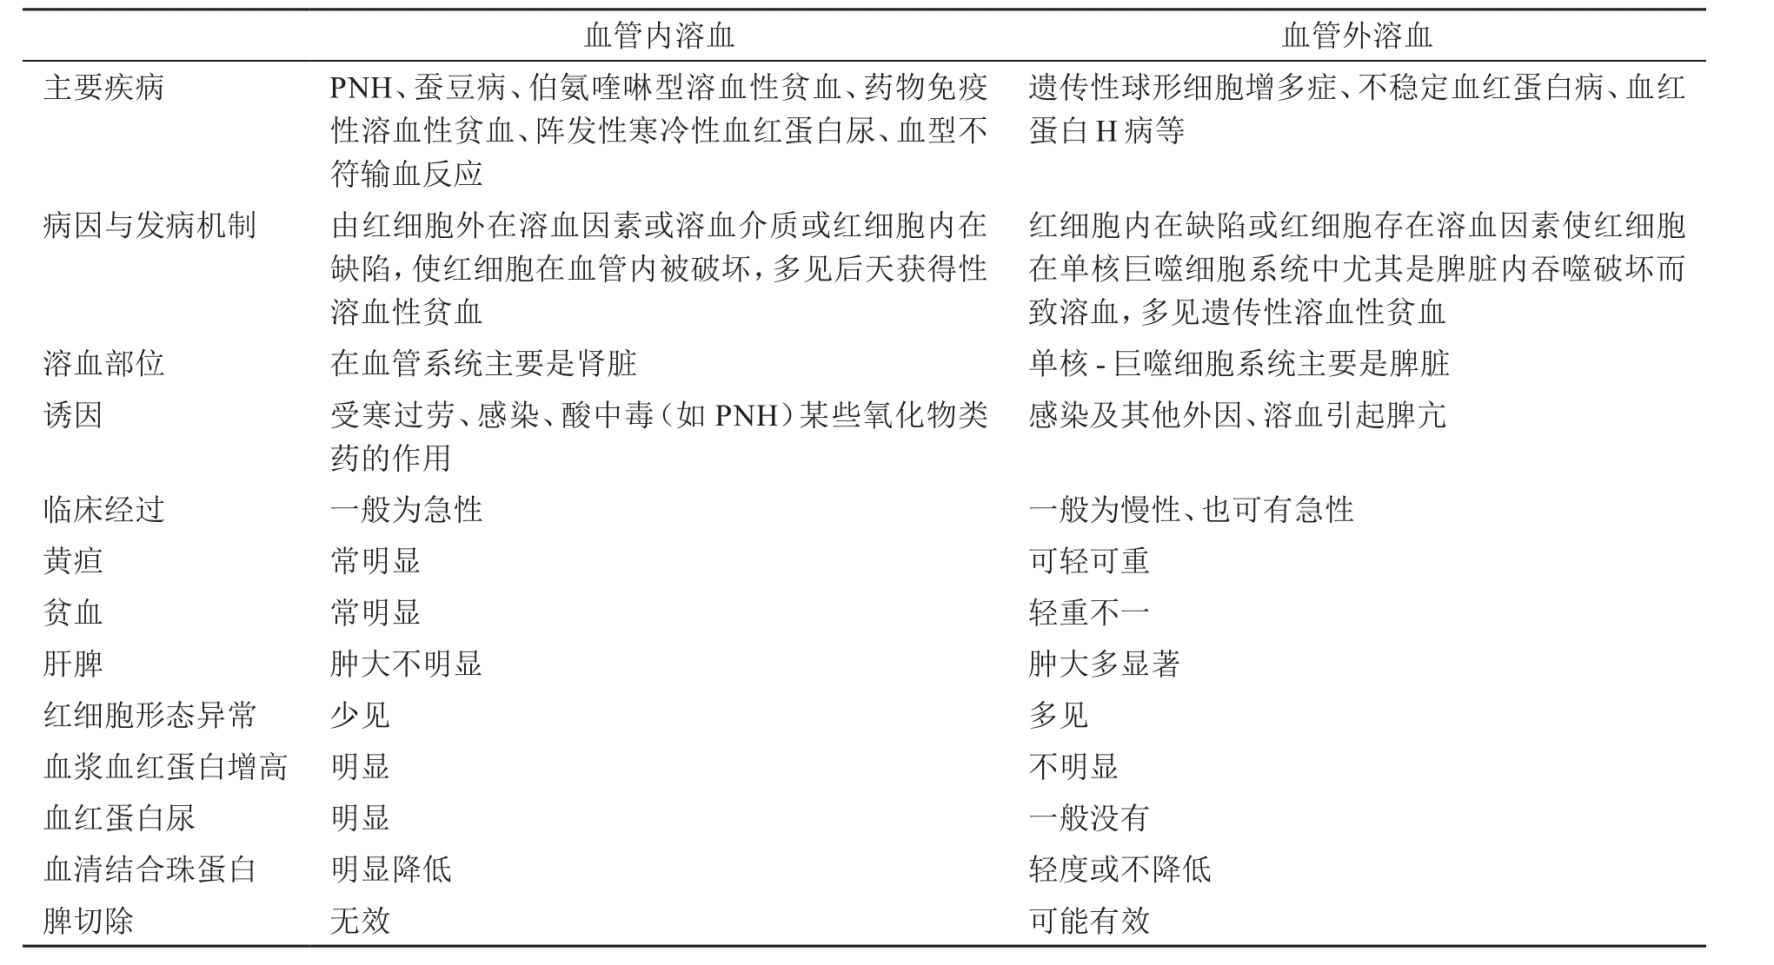
\includegraphics[width=6.79167in,height=3.69792in]{./images/Image00178.jpg}
\end{table}

\subsection{诊断}

\subsubsection{有溶血性贫血的病因和(或)诱因存在}

\subsubsection{临床表现特点}

起病急骤,突出的表现为严重的贫血、黄疸(间接胆红素增加),红细胞寿命缩短,网织红细胞增加,可伴有肝脾肿大。

\paragraph{常有慢性溶血性贫血的原发病的临床症状和体征}

如冷凝集素病患者出现雷诺现象、寒冷性荨麻疹及肢端麻木等;阵发性冷性血红蛋白尿症者,受冷后出现血红蛋白尿和黄疸;阵发性睡眠性血红蛋白尿常在睡眠后出现阵发性溶血等。此外,患者可有面色苍黄、不同程度的黄疸和贫血,轻度全身淋巴结肿大,肝脾肿大尤其以脾大更为明显。

\paragraph{溶血危象期的表现}

其严重程度与不同的病因和病种及溶血方式、溶血的速度等有关。

\hypertarget{text00126.htmlux5cux23CHP4-16-2-2-2-1}{}
(1) 寒战与发热:

大部分危象发生时,先有寒战,继之体温升高,达39℃左右,少数可超过40℃。可有不同程度的烦躁不安、胸闷、谵妄、神志不清。发热可能与红细胞急剧破坏、血红蛋白大量释放有关,有的病例亦可能与危象的感染诱因并存。

\hypertarget{text00126.htmlux5cux23CHP4-16-2-2-2-2}{}
(2) 四肢、腰背、腹部疼痛:

患者多有全身骨痛及腰背酸痛,尤以双肩及两侧肾区疼痛最为显著,腰背疼可以发生在急性肾衰竭之前或之中,并且症状出现越早,肾脏损害越严重。与此同时患者常可伴有腹痛,严重者出现明显的腹肌紧张,酷似急腹症,亦可有恶心、呕吐、腹胀、肠鸣等消化道症状。

\hypertarget{text00126.htmlux5cux23CHP4-16-2-2-2-3}{}
(3) 肾脏损害:

可有少尿或尿闭,高钾血症,氮质血症等,以致发生急性肾衰竭。

\hypertarget{text00126.htmlux5cux23CHP4-16-2-2-2-4}{}
(4) 血压下降:

危象发生后常出现血压下降,甚至休克,同时伴有心率增快,呼吸急促。这与抗原-抗体反应所致的过敏性休克、血管舒缩功能失调有关,尤其在血型不合的输血所致的溶血危象时,血压下降常不易纠正。此外,可因骤然大量溶血,导致高钾血症,心肌缺血缺氧,可引起心律失常,甚至发生心力衰竭。

\hypertarget{text00126.htmlux5cux23CHP4-16-2-2-2-5}{}
(5) 出血倾向与凝血障碍:

大量红细胞破坏可以消耗血液内的凝血物质,发生去纤维蛋白血症综合征(defibrination
syndrome),导致明显的出血倾向。部分患者常因感染、休克、肾功能衰竭、电解质紊乱、酸碱平衡失调并发DIC而使出血加重。

\hypertarget{text00126.htmlux5cux23CHP4-16-2-2-2-6}{}
(6) 贫血加重、黄疸加深:

患者贫血突然加重,全身乏力,心悸气短,危象发生12小时后,可见全身皮肤、黏膜黄疸急剧加深(因一次大量溶血,5~6小时后血中的胆红素浓度可以达到最高峰,但仍需5~6小时皮肤、黏膜才能黄染)。若溶血停止,一般在2~3天后黄疸消退,血中胆红素浓度恢复正常。

\hypertarget{text00126.htmlux5cux23CHP4-16-2-2-2-7}{}
(7) 肝、脾肿大:

溶血危象时,患者的肝脾均有明显肿大,尤其以脾大更为显著,这与贫血及黄疸轻重成正比。急剧肿大的肝、脾常有胀痛和压痛。因大量溶血,胆红素排泄过多,在胆道内沉积,易发生胆结石并发症。

\subsubsection{有溶血性贫血的实验室证据}

\paragraph{红细胞破坏增加的证据}

\hypertarget{text00126.htmlux5cux23CHP4-16-2-3-1-1}{}
(1) 血红蛋白代谢产物增加的表现:

①血清间接胆红素增高;②尿中尿胆原增加,每日可高达5~200mg(正常为0~3.5mg)。

\hypertarget{text00126.htmlux5cux23CHP4-16-2-3-1-2}{}
(2) 血浆血红蛋白含量增高的表现:

①血浆游离血红蛋白含量增高:正常人含量为1~10mg/L,大量溶血时,可高达1000mg/L以上,使血浆颜色变为琥珀色、粉红色或红色。这是血管内溶血最早可观察到的表现。②血清结合珠蛋白降低或消失:血清结合珠蛋白是血液中一组α\textsubscript{2}
糖蛋白,作用似血红蛋白的转运蛋白质。它是在肝脏内产生,正常血清中含量为0.5~1.5g/L(50~150mg/dl)。血管内溶血后,1分子的结合珠蛋白可结合1分子的游离血红蛋白,形成珠蛋白血红蛋白复合物,迅速被肝细胞摄取而从血中消失。大量溶血时,当血浆中游离血红蛋白过多,超过肝脏生成结合珠蛋白的能力,血清结合珠蛋白浓度降低,甚至消失。③血红蛋白尿:游离血红蛋白与结合珠蛋白相结合的产物,由于分子量大,不能通过肾小球排出,但当血浆中游离血红蛋白超过结合珠蛋白所能结合的量,多余的血红蛋白即可从肾小球滤出。经肾小球滤出的游离血红蛋白,在近端肾小管中可部分被重吸收,余下的血红蛋白形成临床所见的血红蛋白尿。所以,所谓血红蛋白的“肾阀”,实际上代表结合珠蛋白结合血红蛋白的能力和肾小管对血红蛋白重吸收能力之和。一般血浆中游离血红蛋白量大于1.3g/L(130mg/dl)时,临床出现血红蛋白尿,尿呈淡红色、红色、棕色或酱油色,尿隐血试验阳性。个别患者结合珠蛋白的表型与血红蛋白结合很差,结合量甚至低达0.025g/L,因而一旦有轻度血管内溶血,很容易出现血红蛋白尿。④含铁血黄素尿:被肾小管重吸收的游离血红蛋白,在肾近曲小管上皮细胞内被分解为卟啉、铁及珠蛋白。超过肾小管上皮细胞所能输送的铁,以铁蛋白或含铁血黄素形式沉积在上皮细胞内。当细胞脱落随尿排出,即成为含铁血黄素尿。血管内溶血后约数天含铁血黄素尿测定才转阳性,并可持续一段时间。⑤高铁血红素白蛋白血症(methemalbuminemia):血浆中游离血红蛋白很易氧化为高铁血红蛋白,然后分解出高铁血红素和珠蛋白,高铁血红素与白蛋白结合成高铁血红素白蛋白,使血浆呈棕色。⑥血清血结素水平降低:血结素系肝内合成,能结合循环中由高铁血红蛋白分解的游离血红素,最后被肝脏清除。血管内溶血时血结素被大量结合而消耗。

\hypertarget{text00126.htmlux5cux23CHP4-16-2-3-1-3}{}
(3) 红细胞寿命缩短:

红细胞的寿命缩短是溶血的最可靠指标。当一般检查不能肯定时,红细胞寿命测定常能显示溶血,且可以估计溶血的严重程度以及鉴别溶血是由于红细胞内缺陷还是红细胞外缺陷,或两者均有缺陷。目前常用有\textsuperscript{15}
Cr、\textsuperscript{3} P-DFP或\textsuperscript{3}
H-DFP(二异丙基氟磷酸)标记红细胞法。

\paragraph{红细胞系代偿性增生的表现}

①网织红细胞增加:溶血性贫血时,因血红蛋白的分解产物刺激造血系统,导致骨髓幼红细胞代偿性增生,网织红细胞一般可达5\%~20\%,如有肯定溶血的患者而无网织红细胞增生者,要考虑有再生障碍性危象的可能性。②周围血液中出现幼红细胞:一般不多,约1\%左右,主要是晚幼红细胞。此外,在严重溶血时尚可见豪-胶(Howell-Jolly)小体和幼粒细胞。由于网织红细胞及其他较不成熟红细胞自骨髓中大量释放至血液,故周围血液中大型红细胞增多。③骨髓幼红细胞增生:溶血性贫血时,幼红细胞显著增生,以中幼和晚幼红细胞最多,形态多正常。粒红比值明显降低(<
1.5)或倒置<
0.5)。④红细胞寿命的化学标志:最常用的代表红细胞寿命的化学标志是红细胞肌酐。较幼稚的红细胞肌酐是成熟型的6~9倍,且持续时间较网织红细胞长。⑤血浆铁转运率(PITR):被用来测定红细胞总的增生程度,且相关性较好。

\subsubsection{确定溶血性贫血的病因}

引起溶血性贫血的原因很多,下列几点可供参考:①若有肯定的化学、物理因素的接触史或明确的感染史,一般病因诊断容易肯定。②抗人球蛋白试验阳性者,应首先考虑免疫性溶血性贫血,进一步探究原因,并用血清学方法以探索抗体的性质。③抗人球蛋白试验阴性,血片中发现大量球形细胞,患者很可能为遗传性球形细胞增多症,可进一步检查红细胞渗透性脆性试验及自体溶血试验,同时进行直系亲属的血象检查以肯定诊断。但球形细胞增多也可见于免疫性溶血性贫血及某些化学及感染因素所致者。④周围血片发现有特殊红细胞畸形者,如椭圆形细胞、大量红细胞碎片、靶形及低色素细胞,可相应考虑遗传性椭圆形细胞增多症、微血管病性溶血性贫血及海洋性贫血,并进行有关的各项检查以肯定之。⑤患者既无红细胞畸形而抗人球蛋白试验又阴性,可进行血红蛋白电泳以除外血红蛋白病;热变性试验以除外不稳定血红蛋白;高铁血红蛋白还原试验以除外红细胞葡萄糖-6-磷酸脱氢酶缺陷症。

\subsubsection{诊断注意事项}

在诊断溶血危象时,应注意与以下疾病相鉴别:

\paragraph{急性再生障碍性贫血}

本病常多凶险,严重进行性贫血、出血、感染,常危及生命,但多无黄疸(除败血症外),网织红细胞明显减少,网织红细胞绝对计数减少,不伴肝脾肿大,骨髓象三系造血严重受抑,非造血细胞增多。

\paragraph{脓毒症}

常有原发或继发感染病灶;有阳性致病菌培养结果;白细胞计数增高且可见中性粒细胞内有中毒颗粒;即使有黄疸也较轻;无血浆中游离血红蛋白增高,无血红蛋白尿。

\paragraph{黄疸型肝炎}

溶血性贫血患者,当某种诱因激发溶血危象时,病情常常特别严重,患者严重乏力、深度黄疸、食欲极度减退伴肝脾肿大,易误诊为黄疸型肝炎,延误治疗。但本病除黄疸外,肝脾可肿大,多为低热,尿胆原可阳性,常无血红蛋白尿,胆红素升高多呈双相反应,网织红细胞多在正常范围内(很少超过5\%),骨髓增生无旺盛改变,末梢血不伴有红细胞受损所致的形态改变。

\paragraph{微血管病性溶血性贫血}

本综合征主要是微血管疾患包括血栓性血小板减少性紫癜、溶血性尿毒症综合征、暴发性紫癜(内毒素血症)等,除溶血表现外,主要是微血管本身病变疾病,各有其原发病特点,溶血只是其中表现之一。

\subsection{治疗}

\subsubsection{治疗病因、消除诱因}

首先应尽量去除已知的病因及各种诱因,如停止血型不合的输血,停用可疑引起溶血的药物、食物,控制感染等。

\subsubsection{肾上腺皮质激素的应用}

肾上腺皮质激素具有抑制单核-巨噬细胞系统合成抗体的作用,并能解脱致敏红细胞上的抗体。使用方便、安全、有效率高,应列为首选药物。主要用于温抗体型自身免疫溶血性贫血(AIHA)的溶血危象,对冷抗体型AIHA无效。对其他非免疫性溶血性贫血疗效不确定,不推荐使用。有适应证者可静脉快速滴注地塞米松20~40mg/d或氢化可的松300~1200mg/d,至少应用3~5天,待急性溶血控制或病情稳定后改用口服。常用泼尼松40~60mg/d口服,当Hb升至100g/L左右时,每周将泼尼松减少5~10mg,减至10~15mg/d时以此量维持1~2个月,最后以5~10mg/d再维持3个月。若在减量过程中,溶血性贫血又加重,应将剂量恢复至最后一次减量前的水平。但大剂量或长期激素治疗常合并高血压、糖尿病、感染,甚至可出现精神异常,必须引起注意。

\subsubsection{输注红细胞}

主要用于急性溶血危象及严重贫血或体质虚弱的患者,目的在于渡过危急难关,暂时改善严重贫血状态。一般输血后约12~48小时病情即可好转;但输血补给了补体有时反而加重溶血,因此,输血时应注意下列各点:①若因大量溶血发生休克、少尿、无尿、急性肾功能衰竭,应先解决少尿、无尿,输入低分子右旋糖酐改善微循环,纠正水、电解质失衡,待尿量增加、肾功能改善后,再进行输血。常需建立两条静脉通道,分别输液和缓慢输浓缩红细胞。②阵发性睡眠性血红蛋白尿接受输入的血浆可激活补体,诱发或加重溶血;严重贫血必须输血时,可谨慎输入经生理盐水洗涤的红细胞。③自体免疫性溶血性贫血患者体内抗体对正常供血者的红细胞易引起凝集现象,使输入的红细胞易于破坏,同时输血还提供了大量的补体,可使溶血加速,故应尽量避免输血。病情必须输血时,应先用配血试验凝集反应最小的供血者血液或经洗涤后红细胞悬液。若病情危急,又急需输血,又无分离或洗涤红细胞的条件,只有在输血的同时应用大量肾上腺皮质激素。输血速度应十分缓慢,密切观察,如有反应,应立即停止输血。④伯氨喹型药物性溶血性贫血及蚕豆病需输血时,献血员应作G-6-PD过筛试验。

\subsubsection{丙种球蛋白的应用}

静脉滴注丙种球蛋白{[}0.2~0.4g/(kg•d){]}对自身免疫性溶血性贫血有短期疗效。

\subsubsection{免疫抑制剂的应用}

免疫抑制剂多用于自身免疫性溶血性贫血对激素无效或需较大剂量维持者,常用环磷酰胺、环孢素和长春新碱等。

\subsubsection{血浆置换疗法}

发生严重贫血者,在静注或静滴皮质激素的同时,如未显效则应及时采取血浆置换疗法,以尽早去除存在于血浆中的抗体,特别适用于免疫性溶血性贫血危象发作时,常可较好较快改善疗效。有条件时应尽早试用。

\subsubsection{预防急性肾衰竭}

急性溶血发生少尿时,在纠正血容量后,为加快游离血红蛋白的排出,应尽早应用甘露醇,以增加肾血流量及尿量。先用20\%甘露醇250ml于15~30分钟内快速静滴完毕,使尿量维持在100ml/h以上。若尿量仍少,应每4~6小时重复1次。24小时尿量应达1500~2400ml。若24小时内仍无尿或少尿,则应停用。呋塞米(速尿)或布美他尼(丁尿胺)可以在用甘露醇的间歇期或甘露醇无效时应用。呋塞米剂量为40~80mg/次静脉注射,必要时可重复使用或加倍量,1天剂量可用至1000mg以上。已发生急性肾衰竭时,治疗原则与其他原因引起的急性肾衰竭相同。

既往处理溶血危象,强调补充碱性液体以碱化尿液,防止肾小管机械性阻塞。目前认为溶血引起肾功能衰竭的原理是反射性的肾血管痉挛,肾血流量减少,肾小管上皮细胞缺血、缺氧、坏死所致;或认为抗原-抗体复合物能引起肾功能损害;或与DIC有关。因此,过多补碱,尤其在少尿或无尿时,有引起碱中毒的潜在危险,使血液pH改变,导致氧解离曲线右移,更不利于组织的氧摄取,甚至可加速肺水肿的发生,故对碱化尿液防治肾衰竭的意义表示怀疑,认为不必列入常规治疗。但一般认为,有血红蛋白尿的患者,在利尿的基础上,适量给予碳酸氢钠来碱化尿液仍是必要的。

\subsubsection{防治其他并发症}

如防治休克、心力衰竭等,参见有关章节。

\subsubsection{脾切除术}

对某些溶血性贫血患者施行脾切除常可收到近期与远期效果,并能减少或防止溶血危象的发生,但须掌握脾切除适应证。对于遗传性球形红细胞增多症、地中海贫血综合征、丙酮酸激酶缺乏、不稳定血红蛋白病和原因不明的自身免疫性溶血性贫血所致的溶血危象,应用大剂量肾上腺皮质激素无效或因其严重副作用而不能耐受治疗,合并显著的脾功能亢进征象,甚至发生溶血危象而不易纠正者,可考虑脾切除术。
\protect\hypertarget{text00127.html}{}{}

\hypertarget{text00127.htmlux5cux23CHP4-16-4}{}
参 考 文 献

1. 顾静文.溶血性贫血概述//陈灏珠,林果为.实用内科学.
第13版.北京:人民卫生出版社,2009:2439

2. 谢毅
.溶血性贫血//陆再英,钟南山.内科学.第7版.北京:人民卫生出版社,2008:582

\protect\hypertarget{text00128.html}{}{}

\chapter{重症肌无力及其危象}

重症肌无力(myasthenia
gravis,MG)是一种神经-肌肉接头传递功能障碍的获得性自身免疫性疾病。主要由于神经-肌肉接头突触后膜上乙酰胆碱受体(acetylcholine
receptors,AChR)受损引起。临床主要表现为部分或全身骨骼肌无力和极易疲劳,具有活动后加重、休息后减轻和晨轻暮重等特点。若在其病程中急骤发生延髓肌和呼吸肌严重无力,出现呼吸困难,以致不能维持换气功能者为重症肌无力危象。其发生率约占MG患者的7.4\%~42.3\%,是神经内科常见急症之一,病死率较高,达19\%~43\%。如能及时、正确抢救,多数可挽回生命。

\subsection{病因与发病机制}

目前研究认为:重症肌无力是对自身Ach受体致敏的自身免疫病。70\%~90\%的重症肌无力患者血清中能检测到抗Ach受体抗体;且大多数患者血清中能检测到抗Ach受体抗体水平与疾病严重程度相一致;血浆置换治疗后,肌无力症状可以暂时好转。重症肌无力与胸腺异常关系密切,80\%以上的重症肌无力患者伴有胸腺异常,其中10\%~20\%的患者为胸腺肿瘤。而33\%~75\%的胸腺瘤患者合并有重症肌无力。胸腺切除以后,70\%的患者临床症状改善。重症肌无力与遗传因素有关,现在研究发现:重症肌无力与人类组织相容抗原(HLA-A,HLA-B,HLA-DR)明显相关。重症肌无力还与内分泌疾病有关,重症肌无力患者常伴发甲状腺功能亢进、类风湿关节炎、系统性红斑狼疮、多发性肌炎、多发性硬化等其他自身免疫性疾病。少数患者有家族性,称为家族性重症肌无力。

重症肌无力是一种主要累及神经-肌肉接头突触后膜AChR的自身免疫性疾病,主要由AChR抗体介导,在细胞免疫和补体参与下突触后膜的AChR被大量破坏,不能产生足够的终板电位,导致突触后膜传递功能障碍而发生肌无力。AChR抗体是一种多克隆抗体,主要成分为IgG,10\%为IgM。在AChR抗体中,直接封闭抗体可以直接竞争性抑制乙酰胆碱(acetylcholine,ACh)与AChR的结合;间接封闭抗体可以干扰ACh与AChR的结合。细胞免疫在MG的发病中也发挥一定的作用,MG患者周围血中辅助性T细胞增多,抑制性T细胞减少,造成B细胞活性增强而产生过量抗体。AChR抗体与AChR的结合还可以通过激活补体而使AChR降解和结构改变,导致突触后膜上的AChR数量减少。最终,神经-肌肉接头的传递功能发生障碍,当连续的神经冲动到来时,不能产生引起肌纤维收缩的动作电位,从而在临床上表现为易疲劳的肌无力。

\subsection{诊断}

\subsubsection{临床表现特点}

本病可见于任何年龄,发病年龄有两个高峰:20~40岁发病者女性多见;40~60岁发病者以男性多见,多合并胸腺瘤。

\paragraph{诱发因素}

感染、过度劳累、情绪波动、精神创伤、妊娠、月经期、系统性疾病、手术等为常见的诱因,甚至可使病情加重。另外一些药物如降低肌肉兴奋性的药物(奎宁、奎尼丁、普鲁卡因胺、利多卡因、苯妥英钠、青霉胺、普萘洛尔等)、止痛剂(吗啡、哌替啶等)、麻醉剂(乙醚、氯化琥珀胆碱、箭毒等)、抗生素(四环素、氨基糖苷类抗生素、新霉素、多黏菌素、巴龙霉素等)、镇静剂(苯二氮{}
类、苯巴比妥、氯丙嗪等)均可严重加重症状或抑制呼吸肌作用,应禁用。

\paragraph{肌无力特点}

受累的骨骼肌主要表现为病态疲劳,即持续活动后肌无力症状明显加重,经短暂休息后症状暂时缓解。肌无力另一特点是症状波动,不仅整个病程有波动,一天中的临床症状有波动,晨起症状较轻,下午和晚上症状逐渐加重,称为晨轻暮重现象。肌无力呈斑片状分布,程度随活动而变化,不能证明符合某一神经或神经根支配区,提示为神经肌肉传导障碍,是MG的典型临床特点。

\paragraph{受累肌的分布与表现}

全身骨骼肌均可受累,多以脑神经支配的肌肉最先受累。肌无力常从一组肌群开始,范围逐步扩大。首发症状常为一侧或双侧眼外肌麻痹,出现眼裂变小、睁眼困难、复视、眼球活动障碍等症状,严重者眼球完全固定,眼内肌(瞳孔括约肌)一般不累及,眼肌症状可以从单眼开始,而后波及对侧,也可双眼同时受累,但双眼症状多不对称。咀嚼肌受累则出现咀嚼无力,尤其在连续咀嚼坚硬食物时更明显,在进餐时常常因肌无力而需要休息,中断进餐,使进餐时间明显延长。咽喉部肌群无力时有吞咽困难,饮水咳呛,讲话时构音困难,常带有鼻音,或声音嘶哑,语音低弱。面肌受累则会有表情呆板,苦笑面容,闭眼和吸吮无力。胸锁乳突肌和斜方肌受累,则出现颈软、抬头困难、转头和耸肩无力。四肢肌肉受累以近端肌无力较远端明显,常呈对称性分布,表现为上臂抬举困难,尤其在做持续性抬举动作如梳头时更明显;下肢无力表现为不能长距离连续行走,常需要中途休息后方可继续前行,因抬腿无力而常需要用手拉住扶手上楼梯,下蹲后起立困难。呼吸肌和膈肌受累时出现咳嗽无力,呼吸困难,严重时可因呼吸肌麻痹而危及生命。偶尔会影响心肌,引起突然死亡。

\paragraph{重症肌无力危象}

大约10\%的重症肌无力出现危象。有三种表现形式:

\hypertarget{text00128.htmlux5cux23CHP4-17-2-1-4-1}{}
(1) 肌无力危象(myasthenic crisis):

在MG病程中,由于某种诱因而致肌无力症状加重,出现呼吸衰竭者为肌无力危象。为最常见的危象,多由于抗胆碱酯酶药物(ChEI)用量不足引起。其诱因多为合并感染、手术或外伤之后、精神创伤、分娩或月经、促皮质素(ACTH)或肾上腺皮质激素应用的早期,以及阻滞神经肌肉传递药物的应用等。上述因素可导致ACh去极化作用受到抑制而致神经兴奋传递障碍,从而使肌无力症状明显加重;咽喉肌及呼吸肌无力,吞咽困难甚至不能进食,呼吸困难,端坐呼吸,呼吸幅度表浅,呼吸频率加快;由于咳痰无力,气管内大量分泌物不能排除而加重缺氧,患者烦躁不安,甚至发生严重发绀。静脉注射依酚氯胺或肌肉注射新斯的明后可使症状明显缓解。

\hypertarget{text00128.htmlux5cux23CHP4-17-2-1-4-2}{}
(2) 胆碱能危象(cholinergic crisis):

由于长期应用ChEI和(或)用量过大,ACh在突触间隙处积聚过多,因而ACh持续作用于AChR,使突触后膜持续去极化,从而复极化过程受阻,而不能形成有效的动作电位,致全身肌力减弱,包括咽喉肌及呼吸肌无力,出现胆碱能危象。此种危象应用ChEI无效,甚至使症状更加严重。胆碱能危象除有呼吸衰竭等肌无力危象表现之外,尚可见有明显的ChEI副作用所致的症状,如流泪、全身大汗、唾液增多,咽喉及气管内大量分泌物,可见有肌束震颤或肌肉抽搐、痉挛,也可有瞳孔缩小、腹痛、腹泻、肠鸣音亢进、恶心、呕吐、尿便失禁等。患者焦虑不安、烦躁、精神错乱,甚至意识障碍、昏迷等。注射阿托品后可使症状改善。停止使用ChEI
24~72小时后临床症状好转。

(3) 反拗危象(brittle
crisis):又称为无反应性危象,是由于突触后膜大量AChR受损,对ChEI失去反应,残余的能与ACh发生反应的AChR太少,致突触后膜难以达到充分的去极化所致。此型可因长期应用ChEI或ChEI的剂量逐渐增大,或因感染、分娩、手术、创伤等诱因而致AChR过度疲劳,对ACh失去反应。临床表现与胆碱能危象相似,但发生此型危象时如应用或停用ChEI等均无效。

上述三种类型危象在病程中并非固定不变,肌无力危象患者在病程中也可能变为胆碱能危象或反拗危象,有的病例即具有胆碱能危象的表现,也有反拗危象的特点,某些病例在临床上不易辨识究竟属于何种类型危象。

\subsubsection{临床分型}

\paragraph{成年型肌无力(Osserman分型)}

Ⅰ型(眼肌型15\%~20\%):仅累及眼外肌,出现上睑下垂、斜视、复视,对肾上腺皮质激素治疗较敏感,大部分预后良好。

Ⅱa型(轻度全身型30\%):可累及眼、面、四肢肌肉,生活多可自理,无明显咽喉肌受累。进展缓慢,对药物敏感。

Ⅱb型(中度全身型25\%):症状较Ⅱa型重,除眼外肌、四肢肌无力外,还有吞咽困难、饮水呛咳、讲话含糊不清等延髓麻痹症状,呼吸肌常不受累,对药物的敏感性欠佳。

Ⅲ型(急性重症型15\%):急性发病,常在数周内累及延髓肌、肢带肌、躯干肌和呼吸肌,肌无力严重,易出现MG危象,此型病死率高。

Ⅳ型(迟发重症型10\%):自Ⅰ、Ⅱa和Ⅱb发展而来,2~4年后累及呼吸肌,症状同Ⅲ型,预后较差,常合并胸腺瘤。

Ⅴ型(伴肌萎缩型):少见,除肌无力外,合并肌萎缩。

\paragraph{少年型肌无力}

指14~18岁之间发病的MG患者,大部分以单纯眼外肌累及为主,仅少部分患者波及咽喉肌和四肢骨骼肌。

\paragraph{新生儿肌无力}

约10\%的MG母亲,其所生的婴儿可有短暂性的MG症状,如哭声低弱、吸吮无力、肌张力低、四肢少动等症状,严重者有呼吸困难,经抗胆碱酯酶药物治疗后,多于1周~3个月内症状消失,此系婴儿通过胎盘获得母体的AChR-Ab
IgG所致。

\paragraph{先天性肌无力}

极少见。婴儿在出生后短期内出现肌无力,持续存在的眼外肌麻痹症状,其母未患MG,但其家族中或同胞兄妹中有MG病史。

\paragraph{药物诱导的肌无力}

见于使用青霉胺治疗的肝豆状核变性、类风湿关节炎等患者中,有典型的MG临床症状,停药后症状可消失。

\subsubsection{辅助诊断试验}

下述试验有助于MG的诊断:

\paragraph{疲劳试验(Jolly试验)}

使受累肌肉在短时间内做重复收缩活动,如肌无力明显加重,经休息后又恢复者,为疲劳试验阳性。如对有上睑下垂者,嘱其持续向上注视,会出现眼睑下垂更明显,而后让其闭目休息数分钟后再睁眼,眼睑下垂症状又改善,为眼肌疲劳试验阳性。对肢体无力者,可令其双臂反复做平举动作,1分钟后出现上臂抬举困难,休息后恢复,为上肢疲劳试验阳性;做反复下蹲后起立动作,1分钟后出现起立越来越慢,甚至不能起立,休息后恢复,为下肢疲劳试验阳性。

\paragraph{抗胆碱酯酶药物试验}

①依酚氯胺(腾喜龙,tensilon)试验:依酚氯胺10mg用注射用水稀释至1ml,先静脉注射2mg,观察20秒,如无出汗、唾液增多等不良反应,再注射8mg(30秒内),1分钟内肌无力症状好转为阳性,持续10分钟后又恢复原状。②新斯的明试验:对依酚氯胺试验可疑者,可作本项试验,因其有较长时间供观察。肌肉注射新斯的明0.5~1mg,起效较慢,10~30分钟达高峰,作用持续2小时。若注射20分钟后肌无力症状好转,为新斯的明试验阳性。如出现恶心、呕吐、腹痛、腹泻、出汗、流涎、瞳孔缩小、心动过缓等毒蕈碱样反应,可肌肉注射阿托品0.5mg予以抵抗。

\subsubsection{辅助检查}

1.血 、尿、脑脊液检查正常。常规肌电图检查基本正常。神经传导速度正常。

2.重复神经电刺激(RNES)
为常用的具有确诊价值的检查方法。90\%的MG患者低频刺激时为阳性,且与病情轻重相关。

3.AChR抗体检测 对MG的诊断具有特征性意义。85\%以上全身型
MG患者血清中AChR抗体明显升高。

4.胸腺影像学检查
胸部X线尤其是胸腺CT和MRI有助于胸腺增生、肥大及胸腺瘤的发现。

\subsubsection{诊断注意事项}

MG的诊断要点:①病史特点:骨骼肌病态疲劳,症状波动,晨轻暮重,活动后加重,休息后减轻,没有神经系统其他阳性体征。②疲劳试验阳性。③新斯的明试验或依酚氯胺试验阳性。④神经重复频率刺激,动作电位波幅递减达10\%以上。⑤血AChR-Ab滴度增高。⑥胸部X线、CT
和MRI可显示胸腺增生或胸腺瘤。⑦服用抗胆碱酯酶药物有效。

MG须与Lambert-Eaton肌无力综合征、肉毒杆菌中毒、肌营养不良症、多发性肌炎等疾病鉴别。

\subsection{治疗}

临床上一旦明确MG诊断,应给予抗胆碱酯酶药物治疗,如单一抗胆碱酯酶药物疗效不明显,可联合应用肾上腺皮质激素或免疫抑制剂、胸腺切除、血浆置换疗法进行综合治疗。除病因及对症处理外,同时应尽量避免本病的各种诱发因素,防治各种感染,对可导致本病加重的药物应禁用或慎用。

\paragraph{抗胆碱酯酶药物}

应从小剂量开始,逐步加量,以能维持日常起居为宜。常用药物有:①溴吡斯的明30~120mg,每天3~4次,口服,作用持续时间6~8小时;②新斯的明15~30mg,每天3~4次,口服,作用维持3~4小时;③安贝氯铵5~10mg,每天3~4次,口服,作用维持4~6小时。以溴吡斯的明最为常用。氯化钾(1g,每天3次,口服)、麻黄碱(25mg,每天3次,口服)等能增强抗胆碱酯酶的作用,可作为辅助性用药。

\paragraph{肾上腺皮质激素}

可抑制自身免疫反应,减少AChR抗体的生成,增加突触前膜ACh的释放量及促使运动终板再生和修复,改善神经-肌肉接头的传递功能。适用于各种类型的MG。用法有两种:①冲击疗法:甲泼尼龙1000mg/d静脉滴注,3~5天后改用地塞米松10~20mg/d静脉滴注,连续7~10天。临床症状稳定改善后,改为口服泼尼松60~100mg隔日晨顿服。当症状基本消失后,逐渐减量至5~15mg长期维持,至少1年以上。适用于重症患者,特别是气管插管、使用人工呼吸机者,能在短期内获得满意疗效。②小剂量递增疗法:从小剂量开始,隔日晨顿服泼尼松20mg,每周递增10mg,直至隔日晨顿服60~80mg,待症状稳定改善4~5天后,逐渐减量至隔日5~15mg维持数年。此法优点是在用药初期一般不会出现MG症状加重。

\paragraph{免疫抑制剂}

适用于对肾上腺皮质激素疗效不佳或不能耐受,或因有高血压、糖尿病、溃疡病而不能用肾上腺皮质激素者。①环磷酰胺:成人口服50mg,每天2~3次,或200mg/次,每周2~3次静脉注射。儿童口服3~5mg/(kg•d)。可与肾上腺皮质激素合用。②环孢素A:6mg/(kg•d),口服,疗程12个月,治疗2周可见改善,6个月时可获最大改善。③硫唑嘌呤:适用于其他疗法无效的全身型MG。成人50~100mg/d,分2次服用,儿童1~3mg/(kg•d),长期服用,多在服药6~12周有效,6~15个月时达最佳疗效。

\paragraph{胸腺治疗}

①胸腺切除:适用于伴有胸腺肥大和高AChR抗体效价者;伴胸腺瘤的各型MG患者;年轻女性全身型MG患者;对ChEI治疗反应不满意者。约70\%的患者术后症状缓解或治愈。②胸腺放射疗法:对于年老体弱、有严重并发症不宜行胸腺摘除术者或手术后又复发者,可行胸腺深部\textsuperscript{60}
Co放射治疗。

\paragraph{血浆置换疗法}

主要清除血浆中的AChR-Ab及其他免疫复合物等致病因素,使症状迅速缓解。具有起效快、作用显著的特点,但维持时间短,价格昂贵,仅适用于危象和难治性MG。

\paragraph{静脉注射免疫球蛋白(IVIG)}

外源性IgG可以干扰AChR抗体与AChR的结合从而保护AChR不被抗体阻断。IVIG
400mg/(kg•d),每日或隔日一次,5次一个疗程,尤其适用于MG加重期、难治性MG及MG危象的治疗。

\paragraph{危象的处理}

处理的关键主要是:①保持呼吸道通畅,改善通气量,使动脉血氧维持正常水平。一旦发现有呼吸肌麻痹,应立即行气管插管和加压人工呼吸,如短期内症状不改善,则及时行气管切开,给予人工呼吸机辅助呼吸。②应注意避免或减少诱发因素。③积极对症处理,防治肺部感染,维持水电解质平衡。④症状治疗:皮质激素治疗,可给予大剂量甲泼尼龙冲击治疗,500~1000mg/d静脉滴注,3~5天后再逐步递减;如条件允许可行血浆置换疗法或静脉注射免疫球蛋白,争取短期内改善症状。同时应根据不同类型的危象采取相应的抢救措施:①肌无力危象:增加CHEI的剂量,静脉注射依酚氯胺10mg或肌肉注射新斯的明0.5~1.0mg,好转后逐渐改口服剂量,亦可用新斯的明2mg加入500ml液体中静脉滴注。②胆碱能危象:立即停用ChEI,阿托品1~2mg肌肉或2mg/h静脉注射,根据病情可重复使用,直至轻度阿托品化,症状改善后重新调整ChEI剂量,或改用皮质激素等其他治疗方案。③反拗性危象:主要维持生命体征的稳定,积极对症处理,避免或防治感染。停用ChEI,经过一段时间后,如对ChEI有效,则重新调整药物剂量;如对ChEI仍不起反应,则改用其他治疗方案。
\protect\hypertarget{text00129.html}{}{}

\hypertarget{text00129.htmlux5cux23CHP4-17-4}{}
参 考 文 献

1. 张文武.急诊内科学.第2版.北京:人民卫生出版社,2008

2. 贾建平.神经病学.第7版.北京:人民卫生出版社,2008

3. Keesey JC. Clinical evaluation and management of myasthenia gravis.
Muscle Nerve,2004,29(4):404-405

4. Rowland LP. Merritts Neurology. 11\textsuperscript{th} ed. New
York:Lippincott Williams & Wilkins,2005

\protect\hypertarget{text00130.html}{}{}

